%%
%% Copyright (C) 2014 Jeffrey P. Hafner <jphafner@buffalo.edu>
%%
%%  This program is free software: you can redistribute it and/or modify
%%  it under the terms of the GNU General Public License as published by
%%  the Free Software Foundation, either version 3 of the License, or
%%  (at your option) any later version.
%%
%%  This program is distributed in the hope that it will be useful,
%%  but WITHOUT ANY WARRANTY; without even the implied warranty of
%%  MERCHANTABILITY or FITNESS FOR A PARTICULAR PURPOSE.  See the
%%  GNU General Public License for more details.
%%
%%  You should have received a copy of the GNU General Public License
%%  along with this program.  If not, see <http://www.gnu.org/licenses/>.
%%

\documentclass[
    11pt,
    titlepage,
]{scrartcl}

\usepackage{AMCexam}

%% Begin Definitions
%%------------------------------------------------
\newlength{\mylen}
\setlength{\parskip}{0pt} % 1ex plus 0.5ex minus 0.2ex}
\setlength{\parindent}{0pt}

\titlehead{Title Head}
\subject{Subject or Class Name}
\title{Examination Title}
\subtitle{Examination Subtitle \textnumero{}\serialnum}
\author{Dr. Jeffrey Hafner}
\date{\today}
%\thanks{}
\publishers{
    The possession or use of \emph{any} communications device is strictly
        prohibited when taking this examination.
    If you use any communications device, no matter how briefly,
        your examination will be invalidated and no score will be given.

    Use of a non-QWERTY calculator, a ruler of any scale,
        any writing utensil,
        and a protractor are permitted.
    The use of any external reference material is strictly prohibited.
    You will be provided with scrap paper by the proctor,
        you may request more at any time.

    For each statement or question, choose the word or expression that,
        of those given, best completes the statement or answers the question.
    Some questions may require the use of the provided reference tables.
    Record your answers on the provided response sheet
        located on the last page of this booklet.

    Questions using the sign \multiSymbole{} may have zero,
        one or several correct answers.
    All other questions have one correct answer.

    You may write in this booklet as only your response
        sheet will be collected.
    You may \emph{only} use either an HB or \textnumero{}2 graphite pencil,
        or a black ink pen on the response sheet.
    Make no stray marks on the response sheet!

    All questions are weighted evenly for grading purposes.
    Each correct response is worth $+4$ points,
        and each incorrect response is worth $-1$ point.
    Questions using the sign \multiSymbole{} are worth $+4$ or $0$,
        and nothing in-between.
    Points awarded will be the geometric mean of the
        points earned and points available.
    
    This booklet has printed material on the
        recto and verso side of each page.
    \emph{Good Luck!}
}

\graphicspath{{./qbank/halliday/gfx/}{./qbank/serway/gfx/}{./qbank/aapt/gfx/}}

%% Begin Document
%%------------------------------------------------
\begin{document}

%% 319 Questions

%% Serway

%%--------------------------------------------------
%% Serway: Physics for Scientists and Engineers
%%--------------------------------------------------


%% Chapter 05: The Laws of Motion
%%--------------------------------------------------


%% Table of Contents
%%--------------------------------------------------

%% 5.1 The Concept of Force
%% 5.1 Newton's First Law and Inertial Frames
%% 5.1 Mass
%% 5.1 Newton's Second Law
%% 5.1 The Gravitational Force and Weight
%% 5.1 Newton's Third Law
%% 5.1 Some Applications of Newton's Laws
%% 5.1 Forces of Friction


%% Serway Multiple Choice Questions
%%--------------------------------------------------
\element{serway-mc}{
\begin{question}{serway-ch05-q01}
    In the figure below,
    \begin{center}
    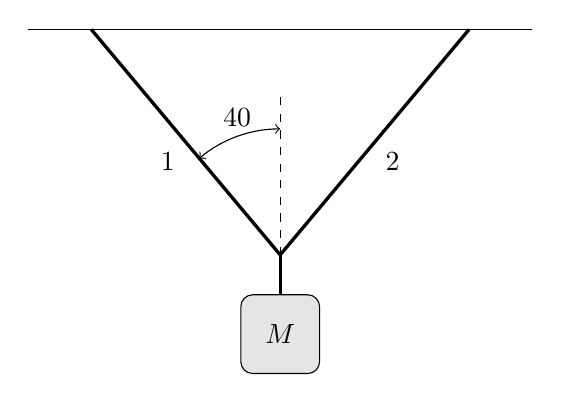
\begin{tikzpicture}[scale=0.8]
        %% Nodes
        \coordinate (A) at (-3,0);
        \coordinate (B) at (+3,0);
        \coordinate (C) at (0,-3.58);
        %% Rope
        \draw (-4,0) -- (4,0);
        \draw[very thick] (A) -- (C) node[anchor=north east,pos=0.5] {1};
        \draw[very thick] (B) -- (C) node[anchor=north west,pos=0.5] {2};
        \draw[dashed] (C) -- ++ (90:2.5);
        \draw[<->] (C) ++ (90:2) arc (90:130:2cm) node[pos=0.5,anchor=south] {\ang{40}};
        %% Mass
        \node[draw,fill=white!90!black,rectangle,rounded corners=1ex,minimum size=1cm,anchor=north,yshift=-0.5cm] (M) at (C) {$M$};
        \draw[very thick] (M.north) -- (C);
    \end{tikzpicture}
    \end{center}
        if the tension in string 1 is \SI{34}{\newton} and the tension in string 2 is \SI{24}{\newton},
        what is the mass of the object shown?
    \begin{multicols}{3}
    \begin{choices}
        \wrongchoice{\SI{7.3}{\kilo\gram}}
        \wrongchoice{\SI{5.5}{\kilo\gram}}
        \wrongchoice{\SI{1.8}{\kilo\gram}}
      \correctchoice{\SI{3.7}{\kilo\gram}}
        \wrongchoice{\SI{4.5}{\kilo\gram}}
    \end{choices}
    \end{multicols}
\end{question}
}

\element{serway-mc}{
\begin{question}{serway-ch05-q02}
    If $M = \SI{2.0}{\kilo\gram}$,
        what is the tension in string 1?
    \begin{center}
    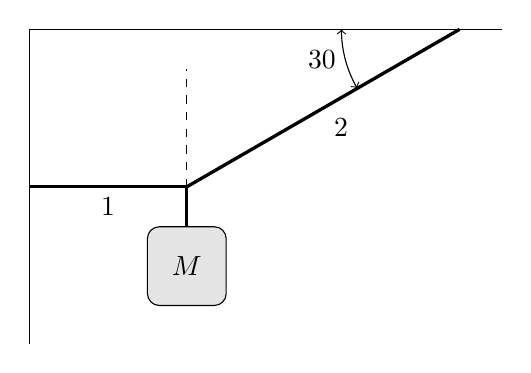
\begin{tikzpicture}
        %% Nodes
        \coordinate (A) at (0,0);
        \coordinate (B) at (+5.464,0);
        \coordinate (C) at (2,-2);
        \coordinate (D) at (0,-2);
        %% Lines
        \draw (0,0) -- (6,0);
        \draw (0,0) -- (0,-4);
        \draw[very thick] (B) --  (C) node[pos=0.5,anchor=north west] {2};
        \draw[very thick] (C) --  (D) node[pos=0.5,anchor=north] {1};
        \draw[dashed] (C) -- ++(90:1.5);
        \draw[<->] (B) ++ (210:1.5) arc (210:180:1.5) node[pos=0.5,anchor=east] {\ang{30}};
        %% Mass
        \node[draw,fill=white!90!black,rectangle,rounded corners=1ex,minimum size=1cm,anchor=north,yshift=-0.5cm] (M) at (C) {$M$};
        \draw[very thick] (M.north) -- (C);
    \end{tikzpicture}
    \end{center}
    \begin{multicols}{3}
    \begin{choices}
        \wrongchoice{\SI{1.2}{\newton}}
        \wrongchoice{\SI{11}{\newton}}
      \correctchoice{\SI{34}{\newton}}
        \wrongchoice{\SI{3.5}{\newton}}
        \wrongchoice{\SI{40}{\newton}}
    \end{choices}
    \end{multicols}
\end{question}
}

\element{serway-mc}{
\begin{question}{serway-ch05-q03}
    If $M = \SI{6.0}{\kilo\gram}$,
        what is the tension in string 1?
    \begin{center}
    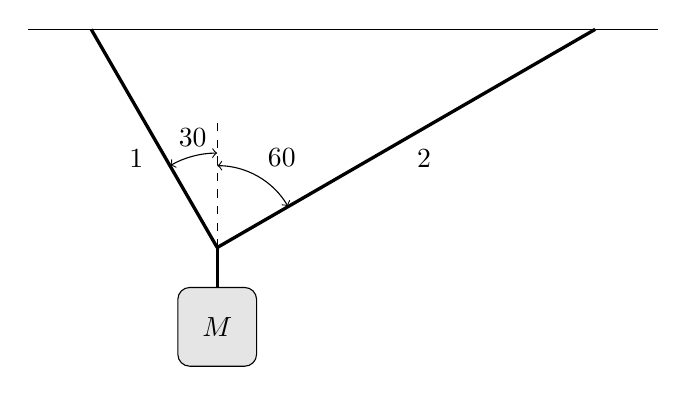
\begin{tikzpicture}[scale=0.8]
        %% Nodes
        \coordinate (A) at (-2,0);
        \coordinate (B) at (+6,0);
        \coordinate (C) at (0,-3.464);
        %% Lines
        \draw (-3,0) -- (7,0);
        \draw[very thick] (B) --  (C) node[pos=0.5,anchor=north west] {2};
        \draw[very thick] (C) --  (A) node[pos=0.5,anchor=north east] {1};
        \draw[dashed] (C) -- ++(90:2.0);
        \draw[<->] (C) ++ (90:1.5) arc (90:120:1.5) node[pos=0.5,anchor=south] {\ang{30}};
        \draw[<->] (C) ++ (90:1.3) arc (90:30:1.3) node[pos=0.5,anchor=south west] {\ang{60}};
        %% Mass
        \node[draw,fill=white!90!black,rectangle,rounded corners=1ex,minimum size=1cm,anchor=north,yshift=-0.5cm] (M) at (C) {$M$};
        \draw[very thick] (M.north) -- (C);
    \end{tikzpicture}
    \end{center}
    \begin{multicols}{3}
    \begin{choices}
        \wrongchoice{\SI{39}{\newton}}
        \wrongchoice{\SI{34}{\newton}}
        \wrongchoice{\SI{29}{\newton}}
        \wrongchoice{\SI{44}{\newton}}
      \correctchoice{\SI{51}{\newton}}
    \end{choices}
    \end{multicols}
\end{question}
}

\element{serway-mc}{
\begin{question}{serway-ch05-q04}
    If $M = \SI{1.1}{\kilo\gram}$,
        what is the tension in string 1?
    \begin{center}
    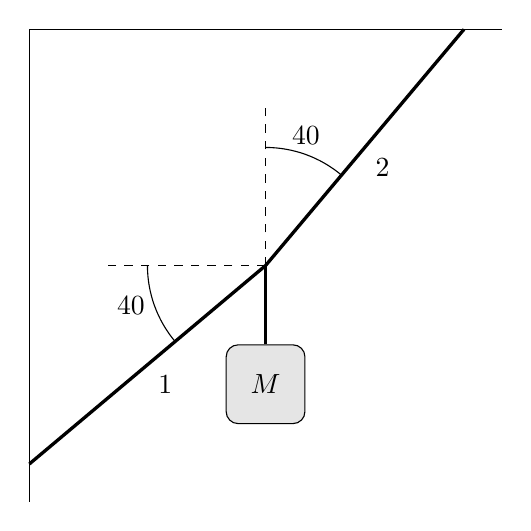
\begin{tikzpicture}
        %% Nodes
        \coordinate (A) at (0,0);
        \coordinate (B) at (+5.52,0);
        \coordinate (C) at (3,-3);
        \coordinate (D) at (0,-5.52);
        %% Lines
        \draw (0,0) -- (6,0);
        \draw (0,0) -- (0,-6);
        \draw[very thick] (B) --  (C) node[pos=0.5,anchor=north west] {2};
        \draw[very thick] (C) --  (D) node[pos=0.5,anchor=north west] {1};
        \draw[dashed] (C) -- ++(90:2.0);
        \draw (C) ++ (90:1.5) arc (90:50:1.5) node[pos=0.5,anchor=south] {\ang{40}};
        \draw (C) ++ (180:1.5) arc (180:220:1.5) node[pos=0.5,anchor=east] {\ang{40}};
        \draw[dashed] (C) -- ++(180:2.0);
        %% Mass
        \node[draw,fill=white!90!black,rectangle,rounded corners=1ex,minimum size=1cm,anchor=north,yshift=-1cm] (M) at (C) {$M$};
        \draw[very thick] (M.north) -- (C);
    \end{tikzpicture}
    \end{center}
    \begin{multicols}{3}
    \begin{choices}
        \wrongchoice{\SI{54}{\newton}}
        \wrongchoice{\SI{47}{\newton}}
      \correctchoice{\SI{40}{\newton}}
        \wrongchoice{\SI{62}{\newton}}
        \wrongchoice{\SI{57}{\newton}}
    \end{choices}
    \end{multicols}
\end{question}
}

\element{serway-mc}{
\begin{question}{serway-ch05-q05}
    An object of unknown weight is suspended as shown. 
    The tension in rope 1 is \SI{25}{\pound},
        and the tension in rope 2 is \SI{31}{\pound}. 
    What is the weight of the suspended object?
    \begin{center}
    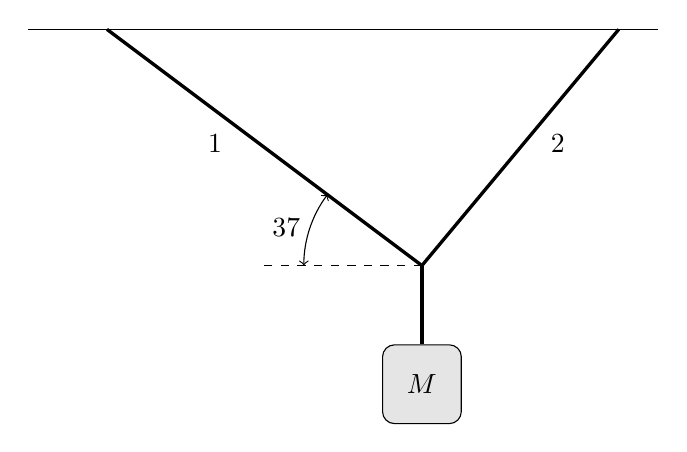
\begin{tikzpicture}
        %% Nodes
        \coordinate (A) at (-4.0,0);
        \coordinate (B) at (2.5,0);
        \coordinate (C) at (0,-3);
        %% Lines
        \draw (-5,0) -- (3,0);
        \draw[very thick] (A) -- (C) node[pos=0.4,anchor=north east] {1};
        \draw[very thick] (B) -- (C) node[pos=0.4,anchor=north west] {2};
        \draw[dashed] (C) -- ++(180:2);
        \draw[<->] (C) ++ (180:1.5) arc (180:143:1.5)
            node[pos=0.5,anchor=east] {\ang{37}};
        %% Mass
        \node[draw,fill=white!90!black,rectangle,rounded corners=1ex,minimum size=1cm,anchor=north,yshift=-1cm] (M) at (C) {$M$};
        \draw[very thick] (M.north) -- (C);
    \end{tikzpicture}
    \end{center}
    \begin{multicols}{3}
    \begin{choices}
        \wrongchoice{\SI{36}{\pound}}
        \wrongchoice{\SI{33}{\pound}}
        \wrongchoice{\SI{41}{\pound}}
      \correctchoice{\SI{39}{\pound}}
        \wrongchoice{\SI{56}{\pound}}
    \end{choices}
    \end{multicols}
\end{question}
}

\element{serway-mc}{
\begin{question}{serway-ch05-q06}
    If $\alpha=\ang{40}$, $\beta=\ang{60}$, and $M=\SI{4.0}{\kilo\gram}$,
        determine the tension in string 1.
    \begin{center}
    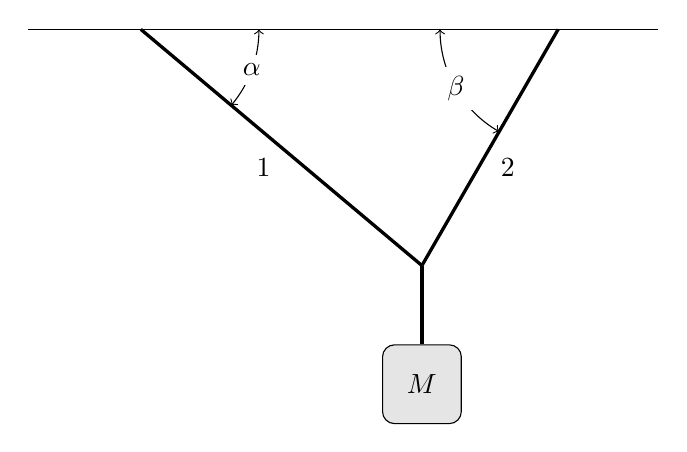
\begin{tikzpicture}
        %% Nodes
        \coordinate (A) at (-3.57,0);
        \coordinate (B) at (1.73,0);
        \coordinate (C) at (0,-3);
        %% Lines
        \draw (-5,0) -- (3,0);
        \draw[very thick] (A) -- (C) node[pos=0.5,anchor=north east] {1};
        \draw[very thick] (B) -- (C) node[pos=0.5,anchor=north west] {2};
        \draw[<->] (A) ++ (0:1.5) arc (0:-40:1.5) node[fill=white,pos=0.5,anchor=center] {$\alpha$};
        \draw[<->] (B) ++ (180:1.5) arc (180:240:1.5) node[fill=white,pos=0.5,anchor=center] {$\beta$};
        %% Mass
        \node[draw,fill=white!90!black,rectangle,rounded corners=1ex,minimum size=1cm,anchor=north,yshift=-1cm] (M) at (C) {$M$};
        \draw[very thick] (M.north) -- (C);
    \end{tikzpicture}
    \end{center}
    \begin{multicols}{3}
    \begin{choices}
        \wrongchoice{\SI{15}{\newton}}
        \wrongchoice{\SI{22}{\newton}}
        \wrongchoice{\SI{17}{\newton}}
      \correctchoice{\SI{20}{\newton}}
        \wrongchoice{\SI{36}{\newton}}
    \end{choices}
    \end{multicols}
\end{question}
}

\element{serway-mc}{
\begin{question}{serway-ch05-q07}
    If $\alpha=\ang{40}$ and the tension in string 2 is \SI{30}{\newton},
        determine $M$.
    \begin{center}
    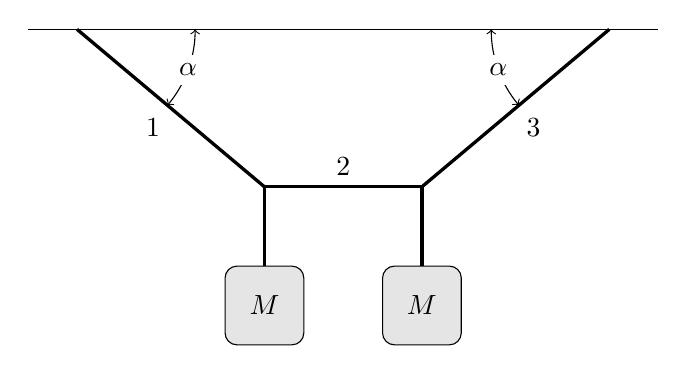
\begin{tikzpicture}
        %% Nodes
        \coordinate (A) at (-3.38,0);
        \coordinate (B) at (+3.38,0);
        \coordinate (C) at (-1,-2);
        \coordinate (D) at (+1,-2);
        %% Lines
        \draw (-4,0) -- (4,0);
        \draw[very thick] (A) -- (C) node[pos=0.5,anchor=north east] {1};
        \draw[very thick] (C) -- (D) node[pos=0.5,anchor=south] {2};
        \draw[very thick] (B) -- (D) node[pos=0.5,anchor=north west] {3};
        \draw[<->] (A) ++ (0:1.5) arc (0:-40:1.5) node[fill=white,pos=0.5,anchor=center] {$\alpha$};
        \draw[<->] (B) ++ (180:1.5) arc (180:220:1.5) node[fill=white,pos=0.5,anchor=center] {$\alpha$};
        %% Mass
        \node[draw,fill=white!90!black,rectangle,rounded corners=1ex,minimum size=1cm,anchor=north,yshift=-1cm] (M) at (C) {$M$};
        \node[draw,fill=white!90!black,rectangle,rounded corners=1ex,minimum size=1cm,anchor=north,yshift=-1cm] (N) at (D) {$M$};
        \draw[very thick] (M.north) -- (C);
        \draw[very thick] (N.north) -- (D);
    \end{tikzpicture}
    \end{center}
    \begin{multicols}{3}
    \begin{choices}
        \wrongchoice{\SI{3.4}{\kilo\gram}}
        \wrongchoice{\SI{3.6}{\kilo\gram}}
      \correctchoice{\SI{2.6}{\kilo\gram}}
        \wrongchoice{\SI{4.9}{\kilo\gram}}
        \wrongchoice{\SI{7.5}{\kilo\gram}}
    \end{choices}
    \end{multicols}
\end{question}
}

\element{serway-mc}{
\begin{question}{serway-ch05-q08}
    Two forces are the only forces acting on a \SI{3.0}{\kilo\gram} object which moves with an acceleration of \SI{3.0}{\meter\per\second\squared} in the positive $y$ direction. 
    If one of the forces acts in the positive $x$ direction and has a magnitude of \SI{8.0}{\newton},
        what is the magnitude of the other force?
    \begin{multicols}{3}
    \begin{choices}
      \correctchoice{\SI{12}{\newton}}
        \wrongchoice{\SI{14}{\newton}}
        \wrongchoice{\SI{16}{\newton}}
        \wrongchoice{\SI{18}{\newton}}
        \wrongchoice{\SI{22}{\newton}}
    \end{choices}
    \end{multicols}
\end{question}
}

\element{serway-mc}{
\begin{question}{serway-ch05-q09}
    The horizontal surface on which the block slides is frictionless. 
    \begin{center}
    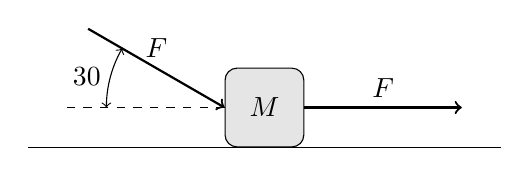
\begin{tikzpicture}
        %% Surface
        \draw (-3,0) -- (3,0);
        %% Block
        \node[draw,fill=white!90!black,rectangle,rounded corners=1ex,minimum size=1cm,anchor=south] (M) at (0,0) {$M$};
        %% Vectors
        \draw[thick,->] (M.east) -- ++(0:2) node[pos=0.5,anchor=south] {$F$};
        \draw[thick,<-] (M.west) -- ++(150:2) node[pos=0.5,anchor=south] {$F$};
        \draw[dashed] (M.west) -- ++(180:2);
        \draw[<->] (M.west) ++(180:1.5) arc (180:150:1.5) node[pos=0.5,anchor=east] {\ang{30}};
    \end{tikzpicture}
    \end{center}
    If $F=\SI{20}{\newton}$ and $M=\SI{5.0}{\kilo\gram}$,
        what is the magnitude of the resulting acceleration of the block?
    \begin{multicols}{3}
    \begin{choices}
        \wrongchoice{\SI{5.3}{\meter\per\second\squared}}
        \wrongchoice{\SI{6.2}{\meter\per\second\squared}}
      \correctchoice{\SI{7.5}{\meter\per\second\squared}}
        \wrongchoice{\SI{4.7}{\meter\per\second\squared}}
        \wrongchoice{\SI{3.2}{\meter\per\second\squared}}
    \end{choices}
    \end{multicols}
\end{question}
}

\element{serway-mc}{
\begin{question}{serway-ch05-q10}
    The only two forces acting on a body have magnitudes of \SI{20}{\newton} and \SI{35}{\newton} and directions that differ by \ang{80}. 
    The resulting acceleration has a magnitude of \SI{20}{\meter\per\second\squared}.
    What is the mass of the body?
    \begin{multicols}{3}
    \begin{choices}
        \wrongchoice{\SI{2.4}{\kilo\gram}}
      \correctchoice{\SI{2.2}{\kilo\gram}}
        \wrongchoice{\SI{2.7}{\kilo\gram}}
        \wrongchoice{\SI{3.1}{\kilo\gram}}
        \wrongchoice{\SI{1.5}{\kilo\gram}}
    \end{choices}
    \end{multicols}
\end{question}
}

\element{serway-mc}{
\begin{question}{serway-ch05-q11}
    If the only forces acting on a \SI{2.0}{\kilo\gram} mass are
        $F_1=\left(3\hat{\imath} - 8\hat{j}\right)\,\si{\newton}$ and
        $F_2=\left(5\hat{\imath} + 3\hat{j}\right)\,\si{\newton}$,
        what is the magnitude of the acceleration of the particle?
    \begin{multicols}{3}
    \begin{choices}
        \wrongchoice{\SI{1.5}{\meter\per\second\squared}}
        \wrongchoice{\SI{6.5}{\meter\per\second\squared}}
      \correctchoice{\SI{4.7}{\meter\per\second\squared}}
        \wrongchoice{\SI{9.4}{\meter\per\second\squared}}
        \wrongchoice{\SI{7.2}{\meter\per\second\squared}}
    \end{choices}
    \end{multicols}
\end{question}
}

\element{serway-mc}{
\begin{question}{serway-ch05-q12}
    At an instant when a \SI{4.0}{\kilo\gram} object has an acceleration equal to $\left(5\hat{\imath} + 3\hat{j}\right)\,\si{\meter\per\second\squared}$,
        one of the two forces acting on the object is known to be $\left(12\hat{\imath} + 22\hat{j}\right)\,\si{\newton}$.
    Determine the magnitude of the other force acting on the object.
    \begin{multicols}{3}
    \begin{choices}
        \wrongchoice{\SI{2.0}{\newton}}
      \correctchoice{\SI{13}{\newton}}
        \wrongchoice{\SI{18}{\newton}}
        \wrongchoice{\SI{1.7}{\newton}}
        \wrongchoice{\SI{20}{\newton}}
    \end{choices}
    \end{multicols}
\end{question}
}

\element{serway-mc}{
\begin{question}{serway-ch05-q13}
    If $F=\SI{4.0}{\newton}$ and $m=\SI{2.0}{\kilo\gram}$,
        what is the magnitude a of the acceleration for the block shown below? 
    \begin{center}
    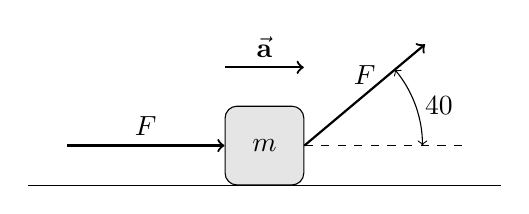
\begin{tikzpicture}
        %% Surface
        \draw (-3,0) -- (3,0);
        %% Block
        \node[draw,fill=white!90!black,rectangle,rounded corners=1ex,minimum size=1cm,anchor=south] (M) at (0,0) {$m$};
        %% ACceleration
        \draw[thick,->] (-0.5,1.5) -- (0.5,1.5) node[pos=0.5,anchor=south] {$\vec{\mathbf{a}}$};
        %% Vectors
        \draw[thick,<-] (M.west) -- ++(180:2) node[pos=0.5,anchor=south] {$F$};
        \draw[thick,->] (M.east) -- ++(40:2) node[pos=0.5,anchor=south] {$F$};
        \draw[dashed] (M.east) -- ++(0:2);
        \draw[<->] (M.east) ++(0:1.5) arc (0:40:1.5) node[pos=0.5,anchor=west] {\ang{40}};
    \end{tikzpicture}
    \end{center}
    The surface is frictionless.
    \begin{multicols}{3}
    \begin{choices}
        \wrongchoice{\SI{5.3}{\meter\per\second\squared}}
        \wrongchoice{\SI{4.4}{\meter\per\second\squared}}
      \correctchoice{\SI{3.5}{\meter\per\second\squared}}
        \wrongchoice{\SI{6.2}{\meter\per\second\squared}}
        \wrongchoice{\SI{8.4}{\meter\per\second\squared}}
    \end{choices}
    \end{multicols}
\end{question}
}

\element{serway-mc}{
\begin{question}{serway-ch05-q14}
    A block is pushed up a frictionless \ang{30} incline by an applied force as shown.
    \begin{center}
    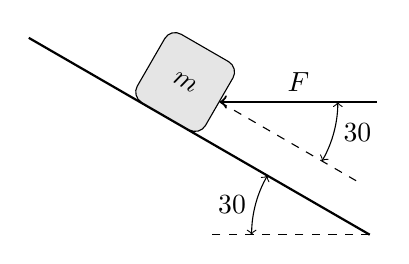
\begin{tikzpicture}
        %% Surface
        \draw[dashed] (0,0) -- (-2,0);
        \draw[thick] (0,0) -- ++ (150:5);
        \draw[<->] (180:1.5) arc (180:150:1.5) node[pos=0.5,anchor=east] {\ang{30}};
        %% Block
        \node[draw,fill=white!90!black,rectangle,rounded corners=1ex,minimum size=1cm,rotate=-30,anchor=south] (M) at (150:3.0) {$m$};
        %% Vectors
        \draw[thick,<-] (M.east) -- ++(0:2) node[pos=0.5,anchor=south] {$F$};
        \draw[dashed] (M.east) -- ++(-30:2);
        \draw[<->] (M.east) ++(-30:1.5) arc (-30:0:1.5) node[pos=0.5,anchor=west] {\ang{30}};
    \end{tikzpicture}
    \end{center}
    If $F=\SI{25}{\newton}$ and $M=\SI{3.0}{\kilo\gram}$,
        what is the magnitude of the resulting acceleration of the block?
    \begin{multicols}{3}
    \begin{choices}
      \correctchoice{\SI{2.3}{\meter\per\second\squared}}
        \wrongchoice{\SI{4.6}{\meter\per\second\squared}}
        \wrongchoice{\SI{3.5}{\meter\per\second\squared}}
        \wrongchoice{\SI{2.9}{\meter\per\second\squared}}
        \wrongchoice{\SI{5.1}{\meter\per\second\squared}}
    \end{choices}
    \end{multicols}
\end{question}
}

\element{serway-mc}{
\begin{question}{serway-ch05-q15}
    A \SI{5.0}{\kilo\gram} object is suspended by a string from the ceiling of an elevator that is accelerating downward at a rate of \SI{2.6}{\meter\per\second\squared}.
    What is the tension in the string?
    \begin{multicols}{3}
    \begin{choices}
        \wrongchoice{\SI{49}{\newton}}
      \correctchoice{\SI{36}{\newton}}
        \wrongchoice{\SI{62}{\newton}}
        \wrongchoice{\SI{13}{\newton}}
        \wrongchoice{\SI{52}{\newton}}
    \end{choices}
    \end{multicols}
\end{question}
}

\element{serway-mc}{
\begin{question}{serway-ch05-q16}
    The tension in a string from which a \SI{4.0}{\kilo\gram} object is suspended in an elevator is equal to \SI{44}{\newton}. 
    What is the acceleration of the elevator?
    \begin{multicols}{2}
    \begin{choices}
        \wrongchoice{\SI{11}{\meter\per\second\squared} upward}
      \correctchoice{\SI{1.2}{\meter\per\second\squared} upward}
        \wrongchoice{\SI{1.2}{\meter\per\second\squared} downward}
        \wrongchoice{\SI{10}{\meter\per\second\squared} upward}
        \wrongchoice{\SI{2.4}{\meter\per\second\squared} downward}
    \end{choices}
    \end{multicols}
\end{question}
}

\element{serway-mc}{
\begin{question}{serway-ch05-q17}
    A \SI{5.0}{\kilo\gram} mass is attached to the ceiling of an elevator by a rope whose mass is negligible. 
    What force does the mass exert on the rope when the elevator has an acceleration of \SI{4.0}{\meter\per\second\squared} upward?
    \begin{multicols}{2}
    \begin{choices}
      \correctchoice{\SI{69}{\newton} downward}
        \wrongchoice{\SI{29}{\newton} downward}
        \wrongchoice{\SI{49}{\newton} downward}
        \wrongchoice{\SI{20}{\newton} downward}
        \wrongchoice{\SI{19}{\newton} downward}
    \end{choices}
    \end{multicols}
\end{question}
}

\element{serway-mc}{
\begin{question}{serway-ch05-q18}
    A \SI{5.0}{\kilo\gram} mass is suspended by a string from the ceiling of an elevator that is moving upward with a speed which is decreasing at a constant rate of \SI{2.0}{\meter\per\second} in each second. 
    What is the tension in the string supporting the mass?
    \begin{multicols}{3}
    \begin{choices}
        \wrongchoice{\SI{49}{\newton}}
      \correctchoice{\SI{39}{\newton}}
        \wrongchoice{\SI{59}{\newton}}
        \wrongchoice{\SI{10}{\newton}}
        \wrongchoice{\SI{42}{\newton}}
    \end{choices}
    \end{multicols}
\end{question}
}

\element{serway-mc}{
\begin{question}{serway-ch05-q19}
    A person weighing \SI{0.70}{\kilo\newton} rides in an elevator that has an upward acceleration of \SI{1.5}{\meter\per\second\squared}. 
    What is the magnitude of the force of the elevator floor on the person?
    \begin{multicols}{3}
    \begin{choices}
        \wrongchoice{\SI{0.11}{\kilo\newton}}
      \correctchoice{\SI{0.81}{\kilo\newton}}
        \wrongchoice{\SI{0.70}{\kilo\newton}}
        \wrongchoice{\SI{0.59}{\kilo\newton}}
        \wrongchoice{\SI{0.64}{\kilo\newton}}
    \end{choices}
    \end{multicols}
\end{question}
}

\element{serway-mc}{
\begin{question}{serway-ch05-q20}
    A \SI{3.0}{\kilo\gram} block slides on a frictionless \ang{20} inclined plane. 
    A force of \SI{16}{\newton} acting parallel to the incline and up the incline is applied to the block. 
    What is the acceleration of the block?
    \begin{choices}
        \wrongchoice{\SI{2.0}{\meter\per\second\squared} down the incline}
        \wrongchoice{\SI{5.3}{\meter\per\second\squared} up the incline}
      \correctchoice{\SI{2.0}{\meter\per\second\squared} up the incline}
        \wrongchoice{\SI{3.9}{\meter\per\second\squared} down the incline}
        \wrongchoice{\SI{3.9}{\meter\per\second\squared} up the incline}
    \end{choices}
\end{question}
}

\element{serway-mc}{
\begin{question}{serway-ch05-q21}
    A \SI{2.0}{\kilo\gram} block slides on a frictionless \ang{25} inclined plane. 
    A force of \SI{4.6}{\newton} acting parallel to the incline and up the incline is applied to the block. 
    What is the acceleration of the block?
    \begin{choices}
        \wrongchoice{\SI{1.8}{\meter\per\second\squared} up the incline}
        \wrongchoice{\SI{2.3}{\meter\per\second\squared} up the incline}
        \wrongchoice{\SI{6.6}{\meter\per\second\squared} down the incline}
      \correctchoice{\SI{1.8}{\meter\per\second\squared} down the incline}
        \wrongchoice{\SI{2.3}{\meter\per\second\squared} down the incline}
    \end{choices}
\end{question}
}

\element{serway-mc}{
\begin{question}{serway-ch05-q22}
    A \SI{2.0}{\kilo\gram} block slides on a frictionless \ang{15} inclined plane. 
    A force acting parallel to the incline is applied to the block. 
    The acceleration of the block is \SI{1.5}{\meter\per\second\squared} down the incline. 
    What is the applied force?
    \begin{choices}
        \wrongchoice{\SI{8.1}{\newton} down the incline}
        \wrongchoice{\SI{3.0}{\newton} down the incline}
      \correctchoice{\SI{2.1}{\newton} up the incline}
        \wrongchoice{\SI{3.0}{\newton} up the incline}
        \wrongchoice{\SI{8.1}{\newton} up the incline}
    \end{choices}
\end{question}
}

\element{serway-mc}{
\begin{question}{serway-ch05-q23}
    A \SI{1.5}{\kilo\gram} object has a velocity of $5\hat{j}\,\si{\meter\per\second}$ at $t = 0$.
    It is accelerated at a constant rate for five seconds after which it has a velocity of $(6\hat{\imath} + 12\hat{j})\,\si{\meter\per\second}$. 
    What is the magnitude of the resultant force acting on the object during this time interval?
    \begin{multicols}{3}
    \begin{choices}
        \wrongchoice{\SI{3.8}{\newton}}
        \wrongchoice{\SI{3.2}{\newton}}
      \correctchoice{\SI{2.8}{\newton}}
        \wrongchoice{\SI{4.3}{\newton}}
        \wrongchoice{\SI{4.6}{\newton}}
    \end{choices}
    \end{multicols}
\end{question}
}

\element{serway-mc}{
\begin{question}{serway-ch05-q24}
    A \SI{1.5}{\kilo\gram} object has a velocity of $5\hat{j}\,\si{\meter\per\second}$ at $t = 0$.
    It is accelerated at a constant rate for five seconds after which it has a velocity of $(6\hat{\imath} + 12\hat{j})\,\si{\meter\per\second}$.
    What is the direction of the resultant force acting on the object during this time interval?
    \begin{multicols}{3}
    \begin{choices}
        \wrongchoice{\ang{65}}
        \wrongchoice{\ang{56}}
        \wrongchoice{\ang{61}}
      \correctchoice{\ang{49}}
        \wrongchoice{\ang{27}}
    \end{choices}
    \end{multicols}
\end{question}
}

\element{serway-mc}{
\begin{question}{serway-ch05-q25}
    A \SI{2.0}{\kilo\gram} object has a velocity of $4.0\hat{\imath}\,\si{\meter\per\second}$ at $t = 0$.
    A constant resultant force of $(2.0\hat{\imath} + 4.0\hat{j})\,\si{\newton}$ then acts on the object for \SI{3.0}{\second}.
    What is the magnitude of the object's velocity at the end of the \SI{3.0}{\second} interval?
    \begin{multicols}{3}
    \begin{choices}
      \correctchoice{\SI{9.2}{\meter\per\second}}
        \wrongchoice{\SI{6.3}{\meter\per\second}}
        \wrongchoice{\SI{8.2}{\meter\per\second}}
        \wrongchoice{\SI{7.2}{\meter\per\second}}
        \wrongchoice{\SI{7.7}{\meter\per\second}}
    \end{choices}
    \end{multicols}
\end{question}
}

\element{serway-mc}{
\begin{question}{serway-ch05-q26}
    A \SI{1.5}{\kilo\gram} mass has an acceleration of
        ${\left(4.0\hat{\imath} - 3.0\hat{j}\right)\,\si{\meter\per\second\squared}}$.
    Only two forces act on the mass. 
    If one of the forces is
        ${\left(2.0\hat{\imath} - 1.4\hat{j}\right)\,\si{\newton}}$,
        what is the magnitude of the other force?
    \begin{multicols}{3}
    \begin{choices}
        \wrongchoice{\SI{4.1}{\newton}}
        \wrongchoice{\SI{6.1}{\newton}}
      \correctchoice{\SI{5.1}{\newton}}
        \wrongchoice{\SI{7.1}{\newton}}
        \wrongchoice{\SI{2.4}{\newton}}
    \end{choices}
    \end{multicols}
\end{question}
}

\element{serway-mc}{
\begin{question}{serway-ch05-q27}
    Only two forces act on a \SI{3.0}{\kilo\gram} mass. 
    One of the forces is \SI{9.0}{\newton} east,
        and the other is \SI{8.0}{\newton} in the direction of \ang{62} north of west. 
    What is the magnitude of the acceleration of the mass?
    \begin{multicols}{3}
    \begin{choices}
        \wrongchoice{\SI{2.0}{\meter\per\second\squared}}
        \wrongchoice{\SI{2.4}{\meter\per\second\squared}}
        \wrongchoice{\SI{3.3}{\meter\per\second\squared}}
      \correctchoice{\SI{2.9}{\meter\per\second\squared}}
        \wrongchoice{\SI{5.7}{\meter\per\second\squared}}
    \end{choices}
    \end{multicols}
\end{question}
}

\element{serway-mc}{
\begin{question}{serway-ch05-q28}
    A book is placed on a chair. 
    Then a videocassette is placed on the book. 
    The floor exerts a normal force
    \begin{choices}
        \wrongchoice{on all three.}
        \wrongchoice{only on the book.}
      \correctchoice{only on the chair.}
        \wrongchoice{upwards on the chair and downwards on the book.}
        \wrongchoice{only on the objects that you have defined to be part of the system.}
    \end{choices}
\end{question}
}

\element{serway-mc}{
\begin{question}{serway-ch05-q29}
    The apparent weight of a fish in an elevator is greatest when the elevator:
    \begin{choices}
        \wrongchoice{moves downward at constant velocity.}
        \wrongchoice{moves upward at constant velocity.}
        \wrongchoice{accelerates downward.}
      \correctchoice{accelerates upward.}
        \wrongchoice{is not moving.}
    \end{choices}
\end{question}
}

\element{serway-mc}{
\begin{question}{serway-ch05-q30}
    The vector sum of three co-planar forces:
    \begin{choices}
        \wrongchoice{must be zero.}
        \wrongchoice{must be perpendicular to one of the three.}
        \wrongchoice{must be parallel to one of the three.}
        \wrongchoice{must be perpendicular to the plane.}
      \correctchoice{may have any direction in the plane.}
    \end{choices}
\end{question}
}

\element{serway-mc}{
\begin{question}{serway-ch05-q31}
    When the vector sum of three co-planar forces, $\mathbf{A}$, $\mathbf{B}$ and $\mathbf{C}$,
        is parallel to $\mathbf{A}$, we can conclude that $\mathbf{B}$ and $\mathbf{C}$:
    \begin{choices}
        \wrongchoice{must sum to zero.}
        \wrongchoice{must be equal and opposite.}
      \correctchoice{must have equal and opposite components perpendicular to $\mathbf{A}$.}
        \wrongchoice{must have equal and opposite components parallel to $\mathbf{A}$.}
        \wrongchoice{must have equal and opposite components parallel and perpendicular to $\mathbf{A}$.}
    \end{choices}
\end{question}
}

\element{serway-mc}{
\begin{question}{serway-ch05-q32}
    A constant force is applied to a body that is already moving. 
    The force is directed at an angle of 60 degrees to the direction of the body's velocity. 
    What is most likely to happen is that
    \begin{choices}
        \wrongchoice{the body will stop moving.}
        \wrongchoice{the body will move in the direction of the force.}
        \wrongchoice{the body's velocity will increase in magnitude but not change direction.}
      \correctchoice{the body will gradually change direction more and more toward that of the force while speeding up.}
        \wrongchoice{the body will first stop moving and then move in the direction of the force.}
    \end{choices}
\end{question}
}

\element{serway-mc}{
\begin{question}{serway-ch05-q33}
    A juggler throws two balls up to the same height so that they pass each other halfway up when $A$ is rising and $B$ is descending. 
    Ignore air resistance and buoyant forces. 
    Which statement is true of the two balls at that point?
    \begin{choices}
        \wrongchoice{There is an residual upward force from the hand on each ball.}
        \wrongchoice{There is a greater residual force from the hand on $A$ than there is on $B$.}
        \wrongchoice{Only gravity acts on $B$ but there is an additional residual force from the hand on $A$.}
        \wrongchoice{There is an additional downwards force besides gravity on each ball.}
      \correctchoice{The only force acting on each ball is the gravitational force.}
    \end{choices}
\end{question}
}

\element{serway-mc}{
\begin{question}{serway-ch05-q34}
    A bumper car is moving at constant velocity when another bumper car starts to push on it with a constant force at an angle of 60 degrees with respect to the first car's initial velocity. 
    The second bumper car continues pushing in exactly that direction for some time. 
    What is most likely to happen is that
    \begin{choices}
        \wrongchoice{the first car will stop moving.}
        \wrongchoice{the first car will move in the direction of the force.}
        \wrongchoice{the first car's velocity will increase in magnitude but not change direction.}
      \correctchoice{the first car's velocity will gradually change direction more and more toward that of the force while increasing in magnitude.}
        \wrongchoice{the first car's velocity will gradually change direction more and more toward that of the force while decreasing in magnitude.}
    \end{choices}
\end{question}
}

\element{serway-mc}{
\begin{question}{serway-ch05-q35}
    You have a machine which can accelerate pucks on frictionless ice. 
    Starting from rest,
        the puck travels a distance $x$ in time $t$ when force $F$ is applied. 
    If force $3F$ is 
        applied, the distance the puck travels in time $t$ is:
    \begin{multicols}{3}
    \begin{choices}
        \wrongchoice{$x$}
        \wrongchoice{$\dfrac{3x}{2}$}
      \correctchoice{$3x$}
        \wrongchoice{$\dfrac{9x}{2}$}
        \wrongchoice{$9x$}
    \end{choices}
    \end{multicols}
\end{question}
}

\element{serway-mc}{
\begin{question}{serway-ch05-q36}
    A constant force $F$ is applied to a body of mass $m$ that initially is headed east at velocity $v_0$ until its velocity becomes $-v_0$. 
    The total time of travel is $2t$. 
    The total distance the body travels in that time is:
    \begin{multicols}{2}
    \begin{choices}
        \wrongchoice{$\dfrac{1}{2}\dfrac{F}{m}t^2$}
      \correctchoice{$\dfrac{F}{m}t^2$}
        \wrongchoice{$v_0t - \dfrac{1}{2}\dfrac{F}{m}t^2$}
        \wrongchoice{$v_0t + \dfrac{1}{2}\dfrac{F}{m}t^2$}
        \wrongchoice{$2\left( v_0t + \dfrac{1}{2}\dfrac{F}{m}t^2\right)$}
    \end{choices}
    \end{multicols}
\end{question}
}

\element{serway-mc}{
\begin{question}{serway-ch05-q37}
    The first of two identical boxes of mass $m$ is sitting on level ground. 
    The second box is sitting on a ramp that makes a \ang{20} angle with the ground. 
    The normal force of the level ground on the first box is $\mathbf{N}_L$;
        the normal force of the ramp on the second box is $\mathbf{N}_R$. 
    Which statement is correct?
    \begin{choices}
        \wrongchoice{$N_R = N_L = mg$}
        \wrongchoice{$N_L = mg$; $N_R = mg\sin\ang{20}.$}
      \correctchoice{$N_L = mg$; $N_R = mg\cos\ang{20}.$}
        \wrongchoice{$N_L = mg$; $N_R = -mg\cos\ang{20}.$}
        \wrongchoice{$N_R = -N_L = -mg$}
    \end{choices}
\end{question}
}

\element{serway-mc}{
\begin{question}{serway-ch05-q38}
    The first of two identical boxes of mass $m$ is sitting on level ground. 
    The second box is sitting on a ramp that makes an angle with the ground. 
    When a force of magnitude $F$ is applied to each box in a direction parallel to the surface it is on,
        upwards on the box on the ramp,
        neither box moves. 
    Which statement comparing the friction force on the box on the level, $f_L$,
        to the friction force on the box on the ramp, $f_R$, is correct?
    \begin{choices}
        \wrongchoice{$f_R = f_L$}
        \wrongchoice{$f_R > f_L$}
      \correctchoice{$f_R < f_L$}
        \wrongchoice{The coefficient of static friction is needed to determine the correct answer.}
        \wrongchoice{The angle between the ramp and the ground is needed to determine the correct answer.}
    \end{choices}
\end{question}
}

\element{serway-mc}{
\begin{question}{serway-ch05-q39}
    The total force needed to drag a box at constant speed across a surface with coefficient of kinetic friction $\mu_k$ is least when the force is applied at an angle $\theta$ such that:
    \begin{multicols}{2}
    \begin{choices}
        \wrongchoice{$\sin\theta = \mu_k$.}
        \wrongchoice{$\cos\theta = \mu_k$.}
        \wrongchoice{$\tan\theta = \mu_k$.}
      \correctchoice{$\cot\theta = \mu_k$.}
        \wrongchoice{$\sec\theta = \mu_k$.}
    \end{choices}
    \end{multicols}
\end{question}
}

\element{serway-mc}{
\begin{question}{serway-ch05-q40}
    A heavy weight is supported by two cables that exert tensions of magnitude $T_1$ and $T_2$.
    \begin{center}
    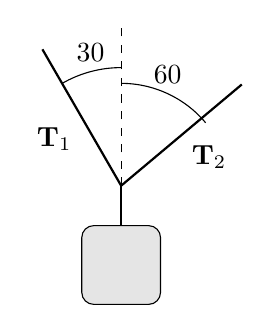
\begin{tikzpicture}
        %% Nodes
        \coordinate (A) at (0,0);
        %% Rope
        \draw[thick] (A) -- ++(40:2) node[pos=0.5,anchor=north west] {$\mathbf{T}_2$};
        \draw[thick] (A) -- ++(120:2) node[pos=0.5,anchor=north east] {$\mathbf{T}_1$};
        \draw[dashed] (A) -- ++(90:2);
        %% Angle
        \draw (A) ++(90:1.5) arc(90:120:1.5) node[pos=0.5,anchor=south] {\ang{30}};
        \draw (A) ++(90:1.3) arc(90:40:1.4) node[pos=0.5,anchor=south] {\ang{60}};
        %% Mass
        \node[draw,fill=white!90!black,rectangle,rounded corners=1ex,minimum size=1cm,anchor=north,yshift=-0.5cm] (M) at (A) {};
        \draw[thick] (M.north) -- (A);
    \end{tikzpicture}
    \end{center}
    Which statement is correct?
    \begin{multicols}{2}
    \begin{choices}
        \wrongchoice{$T_1 = T_2$.}
        \wrongchoice{$T_{1y} = T_{2y}$.}
      \correctchoice{$T_1 > T_2$.}
        \wrongchoice{$T_1 < T_2$.}
        \wrongchoice{We need the mass of the box in order to determine the correct answer.}
    \end{choices}
    \end{multicols}
\end{question}
}

\element{serway-mc}{
\begin{question}{serway-ch05-q41}
    Two people, each of \SI{70}{\kilo\gram} mass, are riding in an elevator. 
    One is standing on the floor. 
    The other is hanging on a rope suspended from the ceiling. 
    Compare the force $F_F$ the floor exerts on the first person to the force $F_R$ the rope exerts on the second person. 
    Which statement is correct?
    \begin{choices}
        \wrongchoice{They are equal and opposite in direction.}
      \correctchoice{The are equal and have the same direction.}
        \wrongchoice{$F_R$ is greater than $F_F$, but they have the same direction.}
        \wrongchoice{$F_R$ is greater than $F_F$, but they have opposite directions.}
        \wrongchoice{$F_R$ is less than $F_F$, but they have the same direction.}
    \end{choices}
\end{question}
}

\element{serway-mc}{
\begin{question}{serway-ch05-q42}
    Two people, each of 70 kg mass, are riding in an elevator. 
    One is standing on the floor. 
    The other is hanging on a rope suspended from the ceiling. 
    Compare the acceleration $a_F$ of the first person to the acceleration $a_R$ of the second person.
    Which statement is correct?
    \begin{choices}
        \wrongchoice{They are equal and opposite in direction.}
      \correctchoice{The are equal and have the same direction.}
        \wrongchoice{The acceleration $a_R$ is greater than $a_F$ , but they have the same direction.}
        \wrongchoice{The acceleration $a_R$ is greater than $a_F$ , but they have opposite directions.}
        \wrongchoice{The acceleration $a_R$ is less than $a_F$ , but they have the same direction.}
    \end{choices}
\end{question}
}

\element{serway-mc}{
\begin{question}{serway-ch05-q43}
    The horizontal surface on which the objects slide is frictionless. 
    \begin{center}
    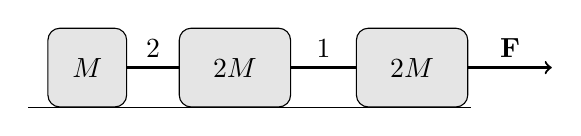
\begin{tikzpicture}[scale=0.75]
        %% Floor
        \draw (-1,0) -- (6.5,0);
        %% Mass
        \node[draw,fill=white!90!black,rectangle,rounded corners=1ex,minimum size=1cm,anchor=south] (A) at (0,0) {$M$};
        \node[draw,fill=white!90!black,rectangle,rounded corners=1ex,minimum width=1.414cm,minimum height=1cm,anchor=south] (B) at (2.5,0) {$2M$};
        \node[draw,fill=white!90!black,rectangle,rounded corners=1ex,minimum width=1.414cm,minimum height=1cm,anchor=south] (C) at (5.5,0) {$2M$};
        %% Rope
        \draw[thick] (A.east) -- (B.west) node[pos=0.5,anchor=south] {2};
        \draw[thick] (B.east) -- (C.west) node[pos=0.5,anchor=south] {1};
        \draw[thick,->] (C.east) -- ++(0:1.414) node[pos=0.5,anchor=south] {$\mathbf{F}$};
    \end{tikzpicture}
    \end{center}
    If $M = \SI{2.0}{\kilo\gram}$,
        the tension in string 1 is \SI{12}{\newton}. 
    Determine $F$.
    \begin{multicols}{3}
    \begin{choices}
        \wrongchoice{\SI{25}{\newton}}
      \correctchoice{\SI{20}{\newton}}
        \wrongchoice{\SI{30}{\newton}}
        \wrongchoice{\SI{35}{\newton}}
        \wrongchoice{\SI{40}{\newton}}
    \end{choices}
    \end{multicols}
\end{question}
}

\element{serway-mc}{
\begin{question}{serway-ch05-q44}
    The horizontal surface on which the objects slide is frictionless. 
    \begin{center}
    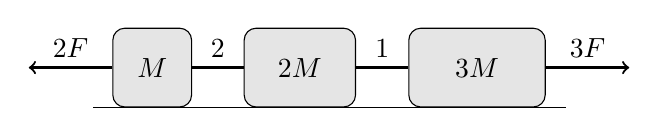
\begin{tikzpicture}[scale=0.75]
        %% Floor
        \draw (-1,0) -- (7,0);
        %% Mass
        \node[draw,fill=white!90!black,rectangle,rounded corners=1ex,minimum size=1cm,anchor=south] (A) at (0,0) {$M$};
        \node[draw,fill=white!90!black,rectangle,rounded corners=1ex,minimum width=1.414cm,minimum height=1cm,anchor=south] (B) at (2.5,0) {$2M$};
        \node[draw,fill=white!90!black,rectangle,rounded corners=1ex,minimum width=1.732cm,minimum height=1cm,anchor=south] (C) at (5.5,0) {$3M$};
        %% Rope
        \draw[thick,->] (A.west) -- ++(180:1.414) node[pos=0.5,anchor=south] {$2F$};
        \draw[thick] (A.east) -- (B.west) node[pos=0.5,anchor=south] {2};
        \draw[thick] (B.east) -- (C.west) node[pos=0.5,anchor=south] {1};
        \draw[thick,->] (C.east) -- ++(0:1.414) node[pos=0.5,anchor=south] {$3F$};
    \end{tikzpicture}
    \end{center}
    If $F=\SI{12}{\newton}$, what is the tension in string 1?
    \begin{multicols}{3}
    \begin{choices}
        \wrongchoice{\SI{35}{\newton}}
      \correctchoice{\SI{30}{\newton}}
        \wrongchoice{\SI{40}{\newton}}
        \wrongchoice{\SI{45}{\newton}}
        \wrongchoice{\SI{25}{\newton}}
    \end{choices}
    \end{multicols}
\end{question}
}

\element{serway-mc}{
\begin{question}{serway-ch05-q45}
    The surface of the inclined plane shown is frictionless. 
    \begin{center}
    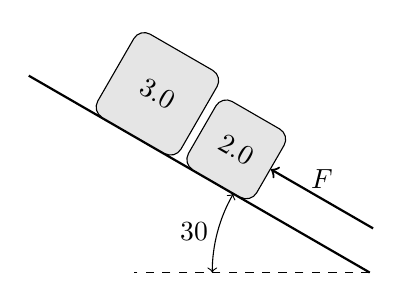
\begin{tikzpicture}
        %% Surface
        \draw[dashed] (0,0) -- (-3,0);
        \draw[thick] (0,0) -- ++ (150:5);
        \draw[<->] (180:2.0) arc (180:150:2.0) node[pos=0.5,anchor=east] {\ang{30}};
        %% Blocks
        \node[draw,fill=white!90!black,rectangle,rounded corners=1ex,minimum size=1.00cm,rotate=-30,anchor=south] (M) at (150:2.25) {\SI{2.0}{\kilo\gram}};
        \node[draw,fill=white!90!black,rectangle,rounded corners=1ex,minimum size=1.22cm,rotate=-30,anchor=south] (N) at (150:3.47) {\SI{3.0}{\kilo\gram}};
        %% Vectors
        \draw[thick,<-] (M.east) -- ++(-30:1.5) node[pos=0.5,anchor=south] {$F$};
    \end{tikzpicture}
    \end{center}
    If $F=\SI{30}{\newton}$,
        what is the magnitude of the force exerted on the \SI{3.0}{\kilo\gram} block by the \SI{2.0}{\kilo\gram} block?
    \begin{multicols}{3}
    \begin{choices}
      \correctchoice{\SI{18}{\newton}}
        \wrongchoice{\SI{27}{\newton}}
        \wrongchoice{\SI{24}{\newton}}
        \wrongchoice{\SI{21}{\newton}}
        \wrongchoice{\SI{15}{\newton}}
    \end{choices}
    \end{multicols}
\end{question}
}

\element{serway-mc}{
\begin{question}{serway-ch05-q46}
    If $P=\SI{6.0}{\newton}$,
        what is the magnitude of the force exerted on block 1 by block 2?
    \begin{center}
    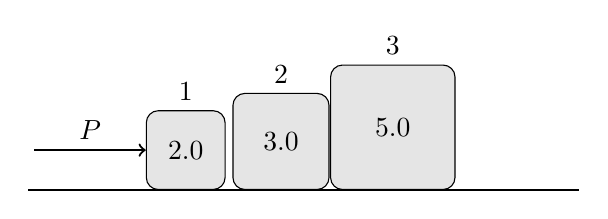
\begin{tikzpicture}
        %% Floor
        \draw (-2,0) -- (5,0);
        %% Mass
        \node[draw,fill=white!90!black,rectangle,rounded corners=1ex,minimum size=1cm,anchor=south] (A) at (0,0) {\SI{2.0}{\kilo\gram}};
        \node[draw,fill=white!90!black,rectangle,rounded corners=1ex,minimum size=1.22cm,anchor=south] (B) at (1.21,0) {\SI{3.0}{\kilo\gram}};
        \node[draw,fill=white!90!black,rectangle,rounded corners=1ex,minimum size=1.58cm,anchor=south] (C) at (2.63,0) {\SI{5.0}{\kilo\gram}};
        %% Labels
        \node[anchor=south] at (A.north) {1};
        \node[anchor=south] at (B.north) {2};
        \node[anchor=south] at (C.north) {3};
        %% Force
        \draw[thick,<-] (A.west) -- ++(180:1.414) node[pos=0.5,anchor=south] {$P$};
    \end{tikzpicture}
    \end{center}
    \begin{multicols}{3}
    \begin{choices}
        \wrongchoice{\SI{6.4}{\newton}}
        \wrongchoice{\SI{5.6}{\newton}}
      \correctchoice{\SI{4.8}{\newton}}
        \wrongchoice{\SI{7.2}{\newton}}
        \wrongchoice{\SI{8.4}{\newton}}
    \end{choices}
    \end{multicols}
\end{question}
}

\element{serway-mc}{
\begin{question}{serway-ch05-q47}
    If $F=\SI{5.0}{\newton}$,
        what is the magnitude of the force exerted by block 2 on block 1?
    \begin{center}
    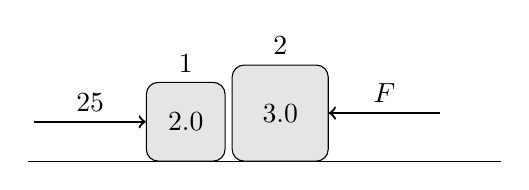
\begin{tikzpicture}
        %% Floor
        \draw (-2,0) -- (4,0);
        %% Mass
        \node[draw,fill=white!90!black,rectangle,rounded corners=1ex,minimum size=1cm,anchor=south] (A) at (0,0) {\SI{2.0}{\kilo\gram}};
        \node[draw,fill=white!90!black,rectangle,rounded corners=1ex,minimum size=1.22cm,anchor=south] (B) at (1.20,0) {\SI{3.0}{\kilo\gram}};
        \node[anchor=south] at (A.north) {1};
        \node[anchor=south] at (B.north) {2};
        %% Force
        \draw[thick,<-] (A.west) -- ++(180:1.414) node[pos=0.5,anchor=south] {\SI{25}{\newton}};
        \draw[thick,<-] (B.east) -- ++(0:1.414) node[pos=0.5,anchor=south] {$F$};
    \end{tikzpicture}
    \end{center}
    \begin{multicols}{3}
    \begin{choices}
      \correctchoice{\SI{17}{\newton}}
        \wrongchoice{\SI{19}{\newton}}
        \wrongchoice{\SI{21}{\newton}}
        \wrongchoice{\SI{23}{\newton}}
        \wrongchoice{\SI{5.0}{\newton}}
    \end{choices}
    \end{multicols}
\end{question}
}

\element{serway-mc}{
\begin{question}{serway-ch05-q48}
    An astronaut who weighs \SI{800}{\newton} on the surface of the earth lifts off from planet Zuton in a space ship. 
    The free-fall acceleration on Zuton is \SI{3.0}{\meter\per\second\squared} (down). 
    At the moment of liftoff the acceleration of the space ship is \SI{0.50}{\meter\per\second\squared} (up). 
    What is the magnitude of the force of the space ship on the astronaut?
    \begin{multicols}{3}
    \begin{choices}
        \wrongchoice{\SI{41}{\kilo\newton}}
      \correctchoice{\SI{0.29}{\kilo\newton}}
        \wrongchoice{\SI{0.24}{\kilo\newton}}
        \wrongchoice{\SI{0.20}{\kilo\newton}}
        \wrongchoice{\SI{0.37}{\kilo\newton}}
    \end{choices}
    \end{multicols}
\end{question}
}

\element{serway-mc}{
\begin{question}{serway-ch05-q49}
    The horizontal surface on which the objects slide is frictionless. 
    \begin{center}
    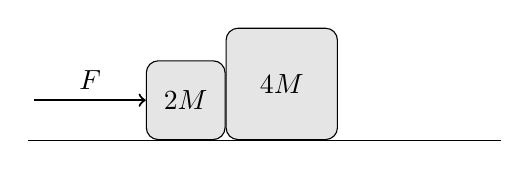
\begin{tikzpicture}
        %% Floor
        \draw (-2,0) -- (4,0);
        %% Mass
        \node[draw,fill=white!90!black,rectangle,rounded corners=1ex,minimum size=1cm,anchor=south] (A) at (0,0) {$2M$};
        \node[draw,fill=white!90!black,rectangle,rounded corners=1ex,minimum size=1.414cm,anchor=south] (B) at (1.22,0) {$4M$};
        %% Force
        \draw[thick,<-] (A.west) -- ++(180:1.414) node[pos=0.5,anchor=south] {$F$};
        %\draw[thick,<-] (B.east) -- ++(0:1.414) node[pos=0.5,anchor=south] {$F$};
    \end{tikzpicture}
    \end{center}
    If $M=\SI{1.0}{\kilo\gram}$ and the magnitude of the force of the   
        small block on the large block is \SI{5.2}{\newton}, determine $F$.
    \begin{multicols}{3}
    \begin{choices}
        \wrongchoice{\SI{6.0}{\newton}}
        \wrongchoice{\SI{9.0}{\newton}}
      \correctchoice{\SI{7.8}{\newton}}
        \wrongchoice{\SI{4.8}{\newton}}
        \wrongchoice{\SI{4.1}{\newton}}
    \end{choices}
    \end{multicols}
\end{question}
}

\element{serway-mc}{
\begin{question}{serway-ch05-q50}
    The horizontal surface on which the objects slide is frictionless. 
    \begin{center}
    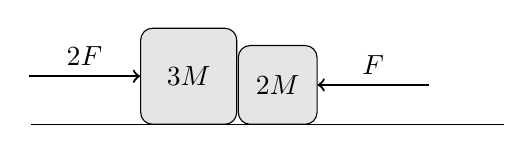
\begin{tikzpicture}
        %% Floor
        \draw (-2,0) -- (4,0);
        %% Mass
        \node[draw,fill=white!90!black,rectangle,rounded corners=1ex,minimum size=1.22cm,anchor=south] (A) at (0,0) {$3M$};
        \node[draw,fill=white!90!black,rectangle,rounded corners=1ex,minimum size=1.00cm,anchor=south] (B) at (1.13,0) {$2M$};
        %% Force
        \draw[thick,<-] (A.west) -- ++(180:1.414) node[pos=0.5,anchor=south] {$2F$};
        \draw[thick,<-] (B.east) -- ++(0:1.414) node[pos=0.5,anchor=south] {$F$};
    \end{tikzpicture}
    \end{center}
    If $F=\SI{6.0}{\newton}$ and $M=\SI{1.0}{\kilo\gram}$,
        what is the magnitude of the force exerted on the large block by the small block?
    \begin{multicols}{3}
    \begin{choices}
        \wrongchoice{\SI{7.7}{\newton}}
        \wrongchoice{\SI{9.8}{\newton}}
        \wrongchoice{\SI{9.1}{\newton}}
      \correctchoice{\SI{8.4}{\newton}}
        \wrongchoice{\SI{6.5}{\newton}}
    \end{choices}
    \end{multicols}
\end{question}
}

\element{serway-mc}{
\begin{question}{serway-ch05-q51}
    A \SI{6.0}{\kilo\gram} object is suspended by a vertical string from the
        ceiling of an elevator which is accelerating upward at a rate of
        \SI{1.8}{\meter\per\second\squared}. 
    Determine the tension in the string.
    \begin{multicols}{3}
    \begin{choices}
        \wrongchoice{\SI{11}{\newton}}
      \correctchoice{\SI{70}{\newton}}
        \wrongchoice{\SI{48}{\newton}}
        \wrongchoice{\SI{59}{\newton}}
        \wrongchoice{\SI{62}{\newton}}
    \end{choices}
    \end{multicols}
\end{question}
}

\element{serway-mc}{
\begin{question}{serway-ch05-q52}
    An \SI{8.0}{\kilo\gram} object rests on the floor of an elevator which is accelerating downward at a rate of \SI{1.3}{\meter\per\second\squared}. 
    What is the magnitude of the force the object exerts on the floor of the elevator?
    \begin{multicols}{3}
    \begin{choices}
        \wrongchoice{\SI{59}{\newton}}
        \wrongchoice{\SI{10}{\newton}}
        \wrongchoice{\SI{89}{\newton}}
      \correctchoice{\SI{68}{\newton}}
        \wrongchoice{\SI{78}{\newton}}
    \end{choices}
    \end{multicols}
\end{question}
}

\element{serway-mc}{
\begin{question}{serway-ch05-q53}
    A \SI{70}{\kilo\gram} stunt artist rides in a rocket sled which slides along a flat inclined surface. 
    At an instant when the sled’s acceleration has a horizontal component of \SI{6.0}{\meter\per\second\squared} and a downward component of \SI{2.8}{\meter\per\second\squared},
        what is the magnitude of the force on the rider by the sled?
    \begin{multicols}{3}
    \begin{choices}
        \wrongchoice{\SI{0.83}{\kilo\newton}}
        \wrongchoice{\SI{0.98}{\kilo\newton}}
      \correctchoice{\SI{0.65}{\kilo\newton}}
        \wrongchoice{\SI{0.68}{\kilo\newton}}
        \wrongchoice{\SI{0.72}{\kilo\newton}}
    \end{choices}
    \end{multicols}
\end{question}
}

\element{serway-mc}{
\begin{question}{serway-ch05-q54}
    If $F=\SI{40}{\newton}$ and $M=\SI{1.5}{\kilo\gram}$,
        what is the tension in the string connecting $M$ and $2M$?
    Assume that all surfaces are frictionless.
    \begin{center}
    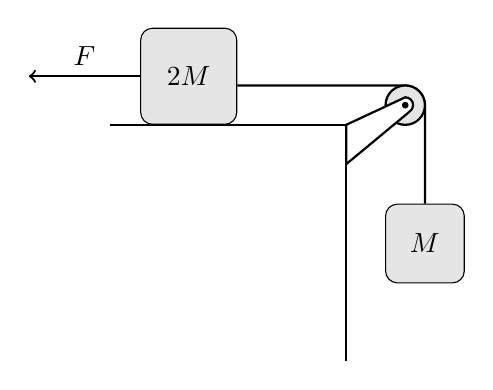
\begin{tikzpicture}
        %% Floor
        \draw[thick] (-3,0) -- (0,0) -- (0,-3);
        %% Mass
        \node[draw,fill=white!90!black,rectangle,rounded corners=1ex,minimum size=1.22cm,anchor=south] (A) at (-2,0) {$2M$};
        \node[draw,fill=white!90!black,rectangle,rounded corners=1ex,minimum size=1.00cm,anchor=north] (B) at (1,-1) {$M$};
        %% Rope and Pulley
        \draw[thick] (A.south east) ++(90:0.5) -- (0.75,0.5) arc(90:0:0.25) -- (B.north);
        \draw[thick,fill=white!90!black] (0.75,0.25) circle (0.25); 
        \draw[thick,fill=white] (0,0) -- (0.75,0.35) arc (90:-60:0.1) -- (0,-0.5) -- cycle;
        \draw[fill] (0.75,0.25) circle (1pt);
        %% Force
        \draw[thick,->] (A.west) -- ++(180:1.414) node[pos=0.5,anchor=south] {$F$};
    \end{tikzpicture}
    \end{center}
    \begin{multicols}{3}
    \begin{choices}
        \wrongchoice{\SI{13}{\newton}}
      \correctchoice{\SI{23}{\newton}}
        \wrongchoice{\SI{36}{\newton}}
        \wrongchoice{\SI{15}{\newton}}
        \wrongchoice{\SI{28}{\newton}}
    \end{choices}
    \end{multicols}
\end{question}
}

\element{serway-mc}{
\begin{question}{serway-ch05-q55}
    The system shown is released from rest and moves \SI{50}{\centi\meter} in \SI{1.0}{\second}.
    What is the value of $M$? 
    All surfaces are frictionless.
    \begin{center}
    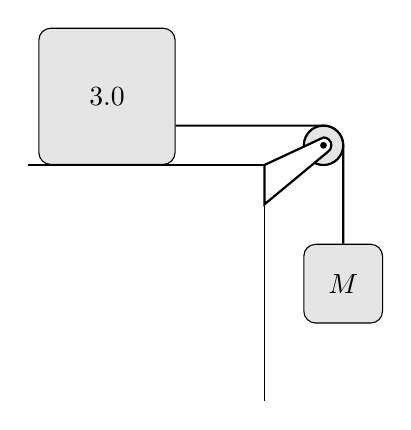
\begin{tikzpicture}
        %% Floor
        \draw (-3,0) -- (0,0) -- (0,-3);
        %% Mass
        \node[draw,fill=white!90!black,rectangle,rounded corners=1ex,minimum size=1.73cm,anchor=south] (A) at (-2,0) {\SI{3.0}{\kilo\gram}};
        \node[draw,fill=white!90!black,rectangle,rounded corners=1ex,minimum size=1.00cm,anchor=north] (B) at (1,-1) {$M$};
        %% Rope and Pulley
        \draw[thick] (A.south east) ++(90:0.5) -- (0.75,0.5) arc(90:0:0.25) -- (B.north);
        \draw[thick,fill=white!90!black] (0.75,0.25) circle (0.25); 
        \draw[thick,fill=white] (0,0) -- (0.75,0.35) arc (90:-60:0.1) -- (0,-0.5) -- cycle;
        \draw[fill] (0.75,0.25) circle (1pt);
    \end{tikzpicture}
    \end{center}
    \begin{multicols}{3}
    \begin{choices}
        \wrongchoice{\SI{0.42}{\kilo\gram}}
      \correctchoice{\SI{0.34}{\kilo\gram}}
        \wrongchoice{\SI{0.50}{\kilo\gram}}
        \wrongchoice{\SI{0.59}{\kilo\gram}}
        \wrongchoice{\SI{0.68}{\kilo\gram}}
    \end{choices}
    \end{multicols}
\end{question}
}

\element{serway-mc}{
\begin{question}{serway-ch05-q56}
    If $F=\SI{40}{\newton}$ and $M=\SI{2.0}{\kilo\gram}$,
        what is the magnitude of the acceleration of the suspended object? 
    All surfaces are frictionless.
    \begin{center}
    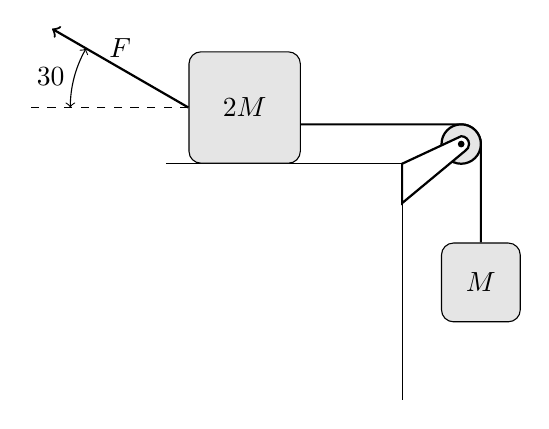
\begin{tikzpicture}
        %% Floor
        \draw (-3,0) -- (0,0) -- (0,-3);
        %% Mass
        \node[draw,fill=white!90!black,rectangle,rounded corners=1ex,minimum size=1.414cm,anchor=south] (A) at (-2,0) {$2M$};
        \node[draw,fill=white!90!black,rectangle,rounded corners=1ex,minimum size=1.00cm,anchor=north] (B) at (1,-1) {$M$};
        %% Rope and Pulley
        \draw[thick] (A.south east) ++(90:0.5) -- (0.75,0.5) arc(90:0:0.25) -- (B.north);
        \draw[thick,fill=white!90!black] (0.75,0.25) circle (0.25); 
        \draw[thick,fill=white] (0,0) -- (0.75,0.35) arc (90:-60:0.1) -- (0,-0.5) -- cycle;
        \draw[fill] (0.75,0.25) circle (1pt);
        %% Force
        \draw[dashed] (A.west) -- ++(180:2);
        \draw[<->] (A.west) ++ (180:1.5) arc(180:150:1.5) node[pos=0.5,anchor=east] {\ang{30}};
        \draw[thick,->] (A.west) -- ++(150:2) node[pos=0.5,anchor=south] {$F$};
    \end{tikzpicture}
    \end{center}
    \begin{multicols}{3}
    \begin{choices}
        \wrongchoice{\SI{1.2}{\meter\per\second\squared}}
        \wrongchoice{\SI{2.0}{\meter\per\second\squared}}
        \wrongchoice{\SI{1.5}{\meter\per\second\squared}}
      \correctchoice{\SI{2.5}{\meter\per\second\squared}}
        \wrongchoice{\SI{5.6}{\meter\per\second\squared}}
    \end{choices}
    \end{multicols}
\end{question}
}

\element{serway-mc}{
\begin{question}{serway-ch05-q57}
    If $M=\SI{2.2}{\kilo\gram}$,
        what is the tension in the connecting string? 
    The pulley and all surfaces are frictionless.
    \begin{center}
    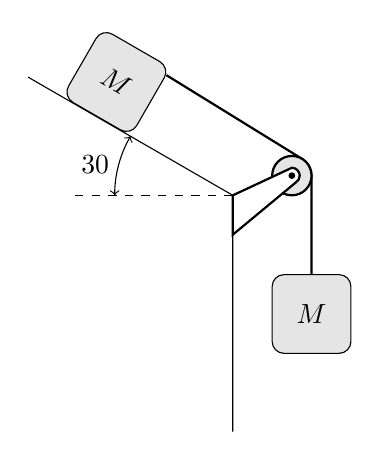
\begin{tikzpicture}
        %% Floor
        \draw (150:3) -- (0,0) -- (0,-3);
        \draw[dashed] (0,0) -- (-2,0);
        \draw[<->] (180:1.5) arc (180:150:1.5) node[pos=0.5,anchor=east] {\ang{30}};
        %% Mass
        \node[draw,fill=white!90!black,rectangle,rounded corners=1ex,minimum size=1cm,rotate=-30,anchor=south] (A) at (150:2) {$M$};
        \node[draw,fill=white!90!black,rectangle,rounded corners=1ex,minimum size=1cm,anchor=north] (B) at (1,-1) {$M$};
        %% Rope and Pulley
        \draw[thick] (A.south east) ++(60:0.9) -- (0.875,0.466) arc(60:0:0.25) -- (B.north);
        \draw[thick,fill=white!90!black] (0.75,0.25) circle (0.25); 
        \draw[thick,fill=white] (0,0) -- (0.75,0.35) arc (90:-60:0.1) -- (0,-0.5) -- cycle;
        \draw[fill] (0.75,0.25) circle (1pt);
    \end{tikzpicture}
    \end{center}
    \begin{multicols}{3}
    \begin{choices}
        \wrongchoice{\SI{6.4}{\newton}}
        \wrongchoice{\SI{5.9}{\newton}}
      \correctchoice{\SI{5.4}{\newton}}
        \wrongchoice{\SI{6.9}{\newton}}
        \wrongchoice{\SI{8.3}{\newton}}
    \end{choices}
    \end{multicols}
\end{question}
}

\element{serway-mc}{
\begin{question}{serway-ch05-q58}
    A \SI{5.0}{\kilo\gram} mass sits on the floor of an elevator that has a downward acceleration of \SI{1.0}{\meter\per\second\squared}.
    On top of the \SI{5.0}{\kilo\gram} mass is an object of unknown mass. 
    The force of the elevator on the \SI{5.0}{\kilo\gram} mass is \SI{80}{\newton} up. 
    Determine the unknown mass.
    \begin{multicols}{3}
    \begin{choices}
        \wrongchoice{\SI{3.3}{\kilo\gram}}
        \wrongchoice{\SI{2.4}{\kilo\gram}}
        \wrongchoice{\SI{1.6}{\kilo\gram}}
      \correctchoice{\SI{4.1}{\kilo\gram}}
        \wrongchoice{\SI{5.0}{\kilo\gram}}
    \end{choices}
    \end{multicols}
\end{question}
}

\element{serway-mc}{
\begin{question}{serway-ch05-q59}
    If the tension, $T$, is \SI{15}{\newton} and the magnitude of the acceleration,
        $a$, is \SI{3.0}{\meter\per\second\squared}, what is the mass, $m$,
        of the suspended object? 
    \begin{center}
    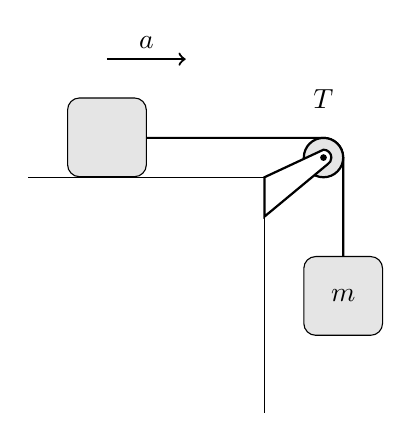
\begin{tikzpicture}
        %% Floor
        \draw (-3,0) -- (0,0) -- (0,-3);
        %% Mass
        \node[draw,fill=white!90!black,rectangle,rounded corners=1ex,minimum size=1.0cm,anchor=south] (A) at (-2,0) {};
        \node[draw,fill=white!90!black,rectangle,rounded corners=1ex,minimum size=1.0cm,anchor=north] (B) at (1,-1) {$m$};
        %% Labels
        \draw[thick,->] (-2,1.5) -- ++ (0:1) node[pos=0.5,anchor=south] {$a$};
        \node[anchor=south] at (0.75,0.75) {$T$};
        %% Rope and Pully
        \draw[thick] (A.south east) ++(90:0.5) -- (0.75,0.5) arc(90:0:0.25) -- (B.north);
        \draw[thick,fill=white!90!black] (0.75,0.25) circle (0.25); 
        \draw[thick,fill=white] (0,0) -- (0.75,0.35) arc (90:-60:0.1) -- (0,-0.5) -- cycle;
        \draw[fill] (0.75,0.25) circle (1pt);
    \end{tikzpicture}
    \end{center}
    Assume that all surfaces and the pulley are frictionless?
    \begin{multicols}{3}
    \begin{choices}
        \wrongchoice{\SI{3.1}{\kilo\gram}}
        \wrongchoice{\SI{2.5}{\kilo\gram}}
        \wrongchoice{\SI{2.8}{\kilo\gram}}
      \correctchoice{\SI{2.2}{\kilo\gram}}
        \wrongchoice{\SI{3.7}{\kilo\gram}}
    \end{choices}
    \end{multicols}
\end{question}
}

\element{serway-mc}{
\begin{question}{serway-ch05-q60}
    If $F=\SI{8.0}{\newton}$ and $M=\SI{1.0}{\kilo\gram}$,
        what is the tension in the connecting string? 
    \begin{center}
    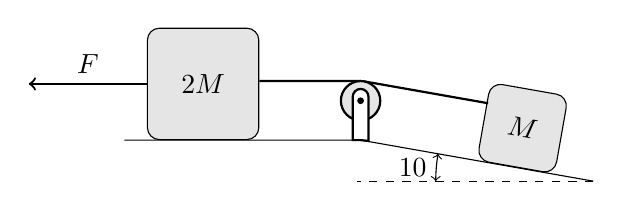
\begin{tikzpicture}
        %% Floor
        \draw (-3,0) -- (0,0) -- ++(350:3);
        \draw[dashed] (350:3) -- ++(180:3);
        \draw[<->] (350:3) ++(180:2) arc (180:170:2) node[pos=0.5,anchor=east] {\ang{10}};
        %% Mass
        \node[draw,fill=white!90!black,rectangle,rounded corners=1ex,minimum size=1.414cm,anchor=south] (A) at (-2,0) {$2M$};
        \node[draw,fill=white!90!black,rectangle,rounded corners=1ex,minimum size=1.0cm,anchor=south,rotate=-10] (B) at (350:2) {$M$};
        %% Rope and Pully
        \draw[thick] (A.south east) ++(90:0.75) -- (0,0.75) arc(90:80:0.25) -- ++(350:1.6);
        \draw[thick,fill=white!90!black] (0,0.5) circle (0.25); 
        \draw[thick,fill=white] (-0.1,0) -- (-0.1,0.55) arc (180:0:0.1) -- (0.1,-0.01) -- (0,0) -- cycle;
        \draw[fill] (0,0.50) circle (1pt);
        %% Forces
        \draw[thick,->] (A.west) -- ++(180:1.5) node[pos=0.5,anchor=south] {$F$};
    \end{tikzpicture}
    \end{center}
    The pulley and all surfaces are frictionless.
    \begin{multicols}{3}
    \begin{choices}
        \wrongchoice{\SI{4.1}{\newton}}
        \wrongchoice{\SI{3.5}{\newton}}
      \correctchoice{\SI{3.8}{\newton}}
        \wrongchoice{\SI{3.1}{\newton}}
        \wrongchoice{\SI{4.8}{\newton}}
    \end{choices}
    \end{multicols}
\end{question}
}

\element{serway-mc}{
\begin{question}{serway-ch05-q61}
    In the figure, if $F=\SI{2.0}{\newton}$ and $M=\SI{1.0}{\kilo\gram}$,
        what is the tension in the connecting string? 
    \begin{center}
    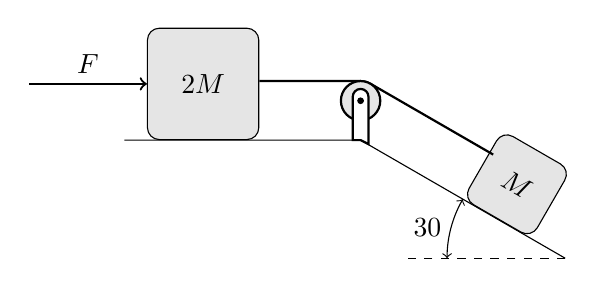
\begin{tikzpicture}
        %% Floor
        \draw (-3,0) -- (0,0) -- ++(330:3);
        \draw[dashed] (330:3) -- ++(180:2);
        \draw[<->] (330:3) ++(180:1.5) arc (180:150:1.5) node[pos=0.5,anchor=east] {\ang{30}};
        %% Mass
        \node[draw,fill=white!90!black,rectangle,rounded corners=1ex,minimum size=1.414cm,anchor=south] (A) at (-2,0) {$2M$};
        \node[draw,fill=white!90!black,rectangle,rounded corners=1ex,minimum size=1.0cm,anchor=south,rotate=-30] (B) at (330:2) {$M$};
        %% Rope and Pully
        \draw[thick] (A.south east) ++(90:0.75) -- (0,0.75) arc(90:60:0.25) -- ++(330:1.8);
        \draw[thick,fill=white!90!black] (0,0.5) circle (0.25); 
        \draw[thick,fill=white] (-0.1,0) -- (-0.1,0.55) arc (180:0:0.1) -- (0.1,-0.05) -- (0,0) -- cycle;
        \draw[fill] (0,0.50) circle (1pt);
        %% Forces
        \draw[thick,<-] (A.west) -- ++(180:1.5) node[pos=0.5,anchor=south] {$F$};
    \end{tikzpicture}
    \end{center}
    The pulley and all surfaces are frictionless.
    \begin{multicols}{3}
    \begin{choices}
      \correctchoice{\SI{2.6}{\newton}}
        \wrongchoice{\SI{1.1}{\newton}}
        \wrongchoice{\SI{2.1}{\newton}}
        \wrongchoice{\SI{1.6}{\newton}}
        \wrongchoice{\SI{3.7}{\newton}}
    \end{choices}
    \end{multicols}
\end{question}
}

\element{serway-mc}{
\begin{question}{serway-ch05-q62}
    A \SI{4.0}{\kilo\gram} block slides down a \ang{35} incline at a constant speed when a \SI{16}{\newton} force is applied acting up and parallel to the incline. 
    What is the coefficient of kinetic friction between the block and the surface of the incline?
    \begin{multicols}{3}
    \begin{choices}
      \correctchoice{\num{0.20}}
        \wrongchoice{\num{0.23}}
        \wrongchoice{\num{0.26}}
        \wrongchoice{\num{0.33}}
        \wrongchoice{\num{0.41}}
    \end{choices}
    \end{multicols}
\end{question}
}

\element{serway-mc}{
\begin{question}{serway-ch05-q63}
    A block is pushed across a horizontal surface by the force shown. 
    \begin{center}
    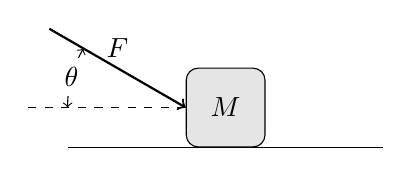
\begin{tikzpicture}
        %% Floor
        \draw (-2,0) -- (2,0);
        %% Mass
        \node[draw,fill=white!90!black,rectangle,rounded corners=1ex,minimum size=1cm,anchor=south] (A) at (0,0) {$M$};
        %% Forces
        \draw[dashed] (A.west) -- ++(180:2);
        \draw[<->] (A.west) ++ (180:1.5) arc (180:150:1.5) node[pos=0.5,anchor=center,fill=white] {$\theta$};
        \draw[thick,<-] (A.west) -- ++(150:2) node[pos=0.5,anchor=south] {$F$};
    \end{tikzpicture}
    \end{center}
    If the coefficient of kinetic friction between the block and the surface is \num{0.30},
        $F=\SI{20}{\newton}$, $\theta=\ang{30}$, and $M=\SI{3.0}{\kilo\gram}$,
        what is the magnitude of the acceleration of the block?
    \begin{multicols}{3}
    \begin{choices}
        \wrongchoice{\SI{2.8}{\meter\per\second\squared}}
        \wrongchoice{\SI{2.3}{\meter\per\second\squared}}
      \correctchoice{\SI{1.8}{\meter\per\second\squared}}
        \wrongchoice{\SI{3.3}{\meter\per\second\squared}}
        \wrongchoice{\SI{5.4}{\meter\per\second\squared}}
    \end{choices}
    \end{multicols}
\end{question}
}

\element{serway-mc}{
\begin{question}{serway-ch05-q64}
    A \SI{3.0}{\kilo\gram} block moves up a \ang{40} incline with constant speed under the action of a \SI{26}{\newton} force acting up and parallel to the incline. 
    What magnitude force must act up and parallel to the incline for the block to move down the incline at constant velocity?
    \begin{multicols}{3}
    \begin{choices}
        \wrongchoice{\SI{14}{\newton}}
      \correctchoice{\SI{12}{\newton}}
        \wrongchoice{\SI{16}{\newton}}
        \wrongchoice{\SI{18}{\newton}}
        \wrongchoice{\SI{25}{\newton}}
    \end{choices}
    \end{multicols}
\end{question}
}

\element{serway-mc}{
\begin{question}{serway-ch05-q65}
    The block shown is pulled across the horizontal surface at a constant speed by the force shown. 
    \begin{center}
    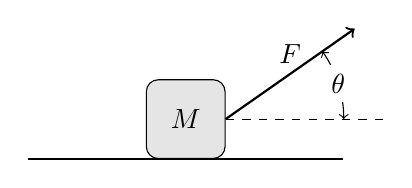
\begin{tikzpicture}
        %% Floor
        \draw (-2,0) -- (2,0);
        %% Mass
        \node[draw,fill=white!90!black,rectangle,rounded corners=1ex,minimum size=1cm,anchor=south] (A) at (0,0) {$M$};
        %% Forces
        \draw[dashed] (A.east) -- ++(0:2);
        \draw[<->] (A.east) ++ (0:1.5) arc (0:35:1.5) node[pos=0.5,anchor=center,fill=white] {$\theta$};
        \draw[thick,->] (A.east) -- ++(35:2) node[pos=0.5,anchor=south] {$F$};
    \end{tikzpicture}
    \end{center}
    If $M=\SI{5.0}{\kilo\gram}$, $F=\SI{14}{\newton}$ and $\theta=\ang{35}$,
        what is the coefficient of kinetic friction between the block and the horizontal surface?
    \begin{multicols}{3}
    \begin{choices}
        \wrongchoice{\num{0.44}}
        \wrongchoice{\num{0.33}}
        \wrongchoice{\num{0.38}}
      \correctchoice{\num{0.28}}
        \wrongchoice{\num{0.17}}
    \end{choices}
    \end{multicols}
\end{question}
}

\element{serway-mc}{
\begin{question}{serway-ch05-q66}
    A box rests on the (horizontal) back of a truck. 
    The coefficient of static friction between the box and the surface on which it rests is \num{0.24}. 
    What maximum distance can the truck travel
        (starting from rest and moving horizontally with constant acceleration)
        in \SI{3.0}{\second} without having the box slide?
    \begin{multicols}{3}
    \begin{choices}
        \wrongchoice{\SI{14}{\meter}}
      \correctchoice{\SI{11}{\meter}}
        \wrongchoice{\SI{19}{\meter}}
        \wrongchoice{\SI{24}{\meter}}
        \wrongchoice{\SI{29}{\meter}}
    \end{choices}
    \end{multicols}
\end{question}
}

\element{serway-mc}{
\begin{question}{serway-ch05-q67}
    In a game of shuffleboard (played on a horizontal surface),
        a puck is given an initial speed of \SI{6.0}{\meter\per\second}. 
    It slides a distance of \SI{9.0}{\meter} before coming to rest. 
    What is the coefficient of kinetic friction between the puck and the surface?
    \begin{multicols}{3}
    \begin{choices}
      \correctchoice{\num{0.20}}
        \wrongchoice{\num{0.18}}
        \wrongchoice{\num{0.15}}
        \wrongchoice{\num{0.13}}
        \wrongchoice{\num{0.27}}
    \end{choices}
    \end{multicols}
\end{question}
}

\element{serway-mc}{
\begin{question}{serway-ch05-q68}
    A \SI{2.0}{\kilo\gram} block slides on a rough horizontal surface. 
    A force (magnitude $P=\SI{4.0}{\newton}$) acting parallel to the surface is applied to the block. 
    The magnitude of the block's acceleration is \SI{1.2}{\meter\per\second\squared}.
    If $P$ is increased to \SI{5.0}{\newton},
        determine the magnitude of the block's acceleration.
    \begin{multicols}{3}
    \begin{choices}
        \wrongchoice{\SI{2.1}{\meter\per\second\squared}}
        \wrongchoice{\SI{2.3}{\meter\per\second\squared}}
        \wrongchoice{\SI{1.9}{\meter\per\second\squared}}
      \correctchoice{\SI{1.7}{\meter\per\second\squared}}
        \wrongchoice{\SI{3.2}{\meter\per\second\squared}}
    \end{choices}
    \end{multicols}
\end{question}
}

\element{serway-mc}{
\begin{question}{serway-ch05-q69}
    A \SI{4.0}{\kilo\gram} block is pushed up a \ang{36} incline by a force of magnitude $P$ applied parallel to the incline. 
    When $P$ is \SI{31}{\newton},
        it is observed that the block moves up the incline with a constant speed. 
    What value of $P$ would be required to lower the block down the incline at a constant speed?
    \begin{multicols}{3}
    \begin{choices}
        \wrongchoice{\SI{27}{\newton}}
      \correctchoice{\SI{15}{\newton}}
        \wrongchoice{\SI{13}{\newton}}
        \wrongchoice{\SI{17}{\newton}}
        \wrongchoice{\SI{19}{\newton}}
    \end{choices}
    \end{multicols}
\end{question}
}

\element{serway-mc}{
\begin{question}{serway-ch05-q70}
    A \SI{1.8}{\kilo\gram} block is released from rest at the top of a rough \ang{30} inclined plane. 
    As the block slides down the incline,
        its acceleration is \SI{3.0}{\meter\per\second\squared} down the incline.
    Determine the magnitude of the force of friction acting on the block.
    \begin{multicols}{3}
    \begin{choices}
        \wrongchoice{\SI{4.2}{\newton}}
        \wrongchoice{\SI{3.0}{\newton}}
      \correctchoice{\SI{3.4}{\newton}}
        \wrongchoice{\SI{3.8}{\newton}}
        \wrongchoice{\SI{2.3}{\newton}}
    \end{choices}
    \end{multicols}
\end{question}
}

\element{serway-mc}{
\begin{question}{serway-ch05-q71}
    A \SI{1.8}{\kilo\gram} block is projected up a rough \ang{10} inclined plane. 
    As the block slides up the incline,
        its acceleration is \SI{3.8}{\meter\per\second\squared} down the incline. 
    What is the magnitude of the force of friction acting on the block?
    \begin{multicols}{3}
    \begin{choices}
        \wrongchoice{\SI{5.0}{\newton}}
      \correctchoice{\SI{3.8}{\newton}}
        \wrongchoice{\SI{4.2}{\newton}}
        \wrongchoice{\SI{4.6}{\newton}}
        \wrongchoice{\SI{6.5}{\newton}}
    \end{choices}
    \end{multicols}
\end{question}
}

\element{serway-mc}{
\begin{question}{serway-ch05-q72}
    A \SI{2.0}{\kilo\gram} block slides on a rough horizontal surface. 
    \begin{center}
    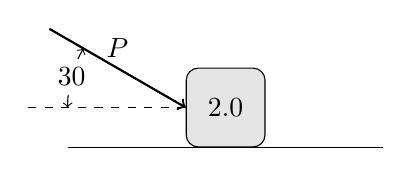
\begin{tikzpicture}
        %% Floor
        \draw (-2,0) -- (2,0);
        %% Mass
        \node[draw,fill=white!90!black,rectangle,rounded corners=1ex,minimum size=1cm,anchor=south] (A) at (0,0) {\SI{2.0}{\kilo\gram}};
        %% Forces
        \draw[dashed] (A.west) -- ++(180:2);
        \draw[<->] (A.west) ++ (180:1.5) arc (180:150:1.5) node[pos=0.5,anchor=center,fill=white] {\ang{30}};
        \draw[thick,<-] (A.west) -- ++(150:2) node[pos=0.5,anchor=south] {$P$};
    \end{tikzpicture}
    \end{center}
    A force ($P=\SI{6.0}{\newton}$) is applied to the block as shown. 
    The magnitude of the block's acceleration is \SI{1.2}{\meter\per\second\squared}.
    What is the magnitude of the force of friction acting on the block?
    \begin{multicols}{3}
    \begin{choices}
        \wrongchoice{\SI{2.0}{\newton}}
        \wrongchoice{\SI{1.4}{\newton}}
        \wrongchoice{\SI{1.6}{\newton}}
      \correctchoice{\SI{2.8}{\newton}}
        \wrongchoice{\SI{3.4}{\newton}}
    \end{choices}
    \end{multicols}
\end{question}
}

\element{serway-mc}{
\begin{question}{serway-ch05-q73}
    A \SI{3.0}{\kilo\gram} block slides on a rough horizontal surface. 
    A force of \SI{8.0}{\newton} acting parallel to the surface is applied to the block. 
    The coefficient of kinetic friction between the block and the surface is \num{0.15}. 
    What is the magnitude of the block's acceleration?
    \begin{multicols}{3}
    \begin{choices}
        \wrongchoice{\SI{1.9}{\meter\per\second\squared}}
      \correctchoice{\SI{1.2}{\meter\per\second\squared}}
        \wrongchoice{\SI{2.3}{\meter\per\second\squared}}
        \wrongchoice{\SI{1.5}{\meter\per\second\squared}}
        \wrongchoice{\SI{2.9}{\meter\per\second\squared}}
    \end{choices}
    \end{multicols}
\end{question}
}

\element{serway-mc}{
\begin{question}{serway-ch05-q74}
    A \SI{1.0}{\kilo\gram} block is pushed up a rough \ang{22} inclined plane by a force of \SI{7.0}{\newton} acting parallel to the incline. 
    The acceleration of the block is \SI{1.4}{\meter\per\second\squared} up the incline.
    Determine the magnitude of the force of friction acting on the block.
    \begin{multicols}{3}
    \begin{choices}
      \correctchoice{\SI{1.9}{\newton}}
        \wrongchoice{\SI{2.2}{\newton}}
        \wrongchoice{\SI{1.3}{\newton}}
        \wrongchoice{\SI{1.6}{\newton}}
        \wrongchoice{\SI{3.3}{\newton}}
    \end{choices}
    \end{multicols}
\end{question}
}

\element{serway-mc}{
\begin{question}{serway-ch05-q75}
    In the figure shown, the coefficient of kinetic friction between the block and the incline is \num{0.29}.
    \begin{center}
    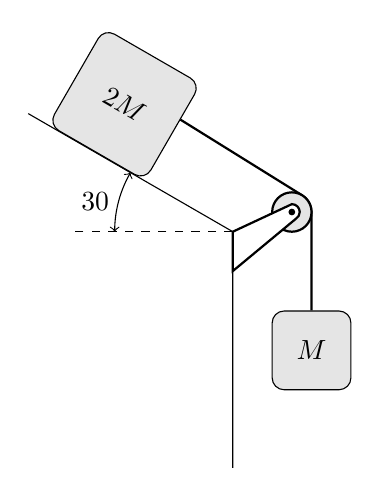
\begin{tikzpicture}
        %% Floor
        \draw (150:3) -- (0,0) -- (0,-3);
        \draw[dashed] (0,0) -- (-2,0);
        \draw[<->] (180:1.5) arc (180:150:1.5) node[pos=0.5,anchor=east] {\ang{30}};
        %% Mass
        \node[draw,fill=white!90!black,rectangle,rounded corners=1ex,minimum size=1.414cm,rotate=-30,anchor=south] (A) at (150:2) {$2M$};
        \node[draw,fill=white!90!black,rectangle,rounded corners=1ex,minimum size=1cm,anchor=north] (B) at (1,-1) {$M$};
        %% Rope and Pully
        \draw[thick] (A.south east) ++(60:0.9) -- (0.875,0.466) arc(60:0:0.25) -- (B.north);
        \draw[thick,fill=white!90!black] (0.75,0.25) circle (0.25); 
        \draw[thick,fill=white] (0,0) -- (0.75,0.35) arc (90:-60:0.1) -- (0,-0.5) -- cycle;
        \draw[fill] (0.75,0.25) circle (1pt);
    \end{tikzpicture}
    \end{center}
    What is the magnitude of the acceleration of the suspended block as it falls? 
    Disregard any pulley mass or friction in the pulley.
    \begin{multicols}{3}
    \begin{choices}
        \wrongchoice{\SI{5.4}{\meter\per\second\squared}}
        \wrongchoice{\SI{5.2}{\meter\per\second\squared}}
      \correctchoice{\SI{4.9}{\meter\per\second\squared}}
        \wrongchoice{\SI{5.6}{\meter\per\second\squared}}
        \wrongchoice{\SI{7.9}{\meter\per\second\squared}}
    \end{choices}
    \end{multicols}
\end{question}
}

\element{serway-mc}{
\begin{question}{serway-ch05-q76}
    In the figure shown, the coefficient of kinetic friction between the block and the incline is \num{0.40}.
    \begin{center}
    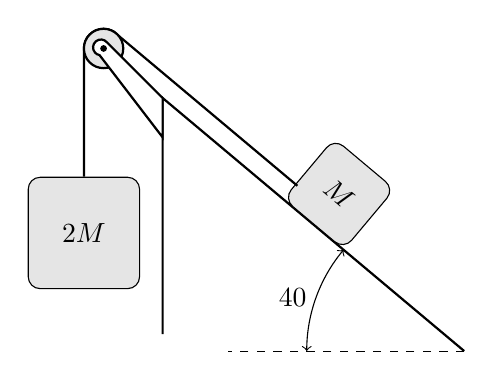
\begin{tikzpicture}
        %% Floor
        \draw[thick] (0,-3) -- (0,0) -- (320:5);
        \draw[dashed] (320:5) -- ++(180:3);
        \draw[<->] (320:5) ++(180:2) arc (180:140:2) node[pos=0.5,anchor=east] {\ang{40}};
        %% Mass
        \node[draw,fill=white!90!black,rectangle,rounded corners=1ex,minimum size=1.414cm,anchor=north] (A) at (-1,-1) {$2M$};
        \node[draw,fill=white!90!black,rectangle,rounded corners=1ex,minimum size=1cm,rotate=-40,anchor=south] (B) at (320:2.5) {$M$};
        %% Rope and Pully
        \draw[thick] (A.north) -- (-1.0,0.629) arc(180:60:0.25) -- ++(320:3.05);
        \draw[thick,fill=white!90!black] (-0.75,0.629) circle (0.25); 
        \draw[thick,fill=white] (0,0) -- ++ (135:1.0) arc (40:260:0.1) -- (0,-0.5) -- cycle;
        \draw[fill] (-0.75,0.629) circle (1pt);
    \end{tikzpicture}
    \end{center}
    What is the magnitude of the acceleration of the suspended block as it falls? 
    Disregard any pulley mass or friction in the pulley.
    \begin{multicols}{3}
    \begin{choices}
      \correctchoice{\SI{3.4}{\meter\per\second\squared}}
        \wrongchoice{\SI{3.7}{\meter\per\second\squared}}
        \wrongchoice{\SI{4.2}{\meter\per\second\squared}}
        \wrongchoice{\SI{3.9}{\meter\per\second\squared}}
        \wrongchoice{\SI{5.4}{\meter\per\second\squared}}
    \end{choices}
    \end{multicols}
\end{question}
}

\element{serway-mc}{
\begin{question}{serway-ch05-q77}
    The three blocks shown are released from rest and are observed to move with accelerations that have a magnitude of \SI{1.5}{\meter\per\second\squared}. 
    \begin{center}
    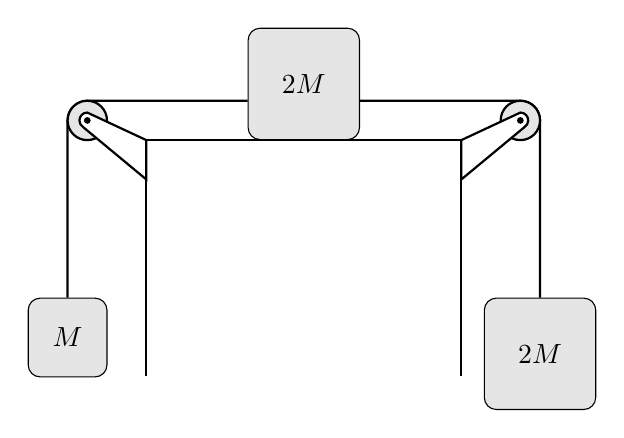
\begin{tikzpicture}
        %% Floor
        \draw[thick] (-2,-3) -- (-2,0) -- (2,0) -- (2,-3);
        %% Mass
        \node[draw,fill=white!90!black,rectangle,rounded corners=1ex,minimum size=1.414cm,anchor=south] (A) at (0,0) {$2M$};
        \node[draw,fill=white!90!black,rectangle,rounded corners=1ex,minimum size=1.414cm,anchor=north] (B) at (3,-2) {$2M$};
        \node[draw,fill=white!90!black,rectangle,rounded corners=1ex,minimum size=1.000cm,anchor=north] (C) at (-3,-2) {$M$};
        %% Rope
        \draw[thick] (A.south east) ++(90:0.5) -- (+2.75,0.5) arc(90:0:0.25) -- (B.north);
        \draw[thick] (A.south west) ++(90:0.5) -- (-2.75,0.5) arc(90:180:0.25) -- (C.north);
        %% Pully
        \draw[thick,fill=white!90!black] (+2.75,0.25) circle (0.25); 
        \draw[thick,fill=white!90!black] (-2.75,0.25) circle (0.25); 
        \draw[thick,fill=white] (2,0) -- (2.75,0.35) arc (90:-60:0.1) -- (2,-0.5) -- cycle;
        \draw[thick,fill=white] (-2,0) -- (-2.75,0.35) arc (90:240:0.1) -- (-2,-0.5) -- cycle;
        \draw[fill] (+2.75,0.25) circle (1pt);
        \draw[fill] (-2.75,0.25) circle (1pt);
    \end{tikzpicture}
    \end{center}
    What is the magnitude of the friction force on the block that slides horizontally? 
    Disregard any pulley mass or friction in the pulley and let $M=\SI{2.0}{\kilo\gram}$.
    \begin{multicols}{3}
    \begin{choices}
        \wrongchoice{\SI{6.0}{\newton}}
        \wrongchoice{\SI{5.1}{\newton}}
        \wrongchoice{\SI{5.5}{\newton}}
      \correctchoice{\SI{4.6}{\newton}}
        \wrongchoice{\SI{3.7}{\newton}}
    \end{choices}
    \end{multicols}
\end{question}
}

\element{serway-mc}{
\begin{question}{serway-ch05-q78}
    Two blocks in contact with each other are pushed to the right across a rough horizontal surface by the two forces shown. 
    \begin{center}
    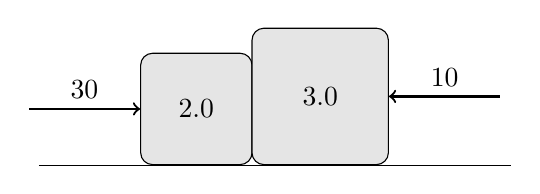
\begin{tikzpicture}
        %% Floor
        \draw (-2,0) -- (4,0);
        %% Mass
        \node[draw,fill=white!90!black,rectangle,rounded corners=1ex,minimum size=1.414cm,anchor=south] (A) at (0,0) {\SI{2.0}{\kilo\gram}};
        \node[draw,fill=white!90!black,rectangle,rounded corners=1ex,minimum size=1.732cm,anchor=south] (B) at (1.573,0) {\SI{3.0}{\kilo\gram}};
        %% Force
        \draw[thick,<-] (A.west) -- ++(180:1.414) node[pos=0.5,anchor=south] {\SI{30}{\newton}};
        \draw[thick,<-] (B.east) -- ++(0:1.414) node[pos=0.5,anchor=south] {\SI{10}{\newton}};
    \end{tikzpicture}
    \end{center}
    If the coefficient of kinetic friction between each of the blocks and the surface is \num{0.30},
        determine the magnitude of the force exerted on the \SI{2.0}{\kilo\gram} block by the \SI{3.0}{\kilo\gram} block.
    \begin{multicols}{3}
    \begin{choices}
        \wrongchoice{\SI{15}{\newton}}
        \wrongchoice{\SI{25}{\newton}}
        \wrongchoice{\SI{11}{\newton}}
      \correctchoice{\SI{22}{\newton}}
        \wrongchoice{\SI{33}{\newton}}
    \end{choices}
    \end{multicols}
\end{question}
}

\element{serway-mc}{
\begin{question}{serway-ch05-q79}
    Two blocks are accelerated across a horizontal frictionless surface as shown.
    Frictional forces keep the two blocks from sliding relative to each other,
        and the two move with the same acceleration.
    \begin{center}
    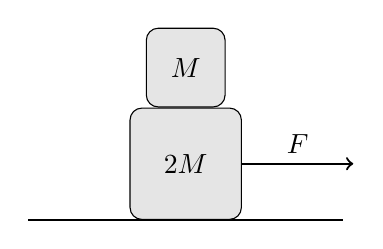
\begin{tikzpicture}
        %% Floor
        \draw (-2,0) -- (2,0);
        %% Mass
        \node[draw,fill=white!90!black,rectangle,rounded corners=1ex,minimum size=1.414cm,anchor=south] (A) at (0,0) {$2M$};
        \node[draw,fill=white!90!black,rectangle,rounded corners=1ex,minimum size=1.000cm,anchor=south] (B) at (A.north) {$M$};
        %% Force
        \draw[thick,->] (A.east) -- ++(0:1.414) node[pos=0.5,anchor=south] {$F$};
    \end{tikzpicture}
    \end{center}
    If $F=\SI{1.2}{\newton}$ and $M=\SI{1.0}{\kilo\gram}$,
        what is the horizontal component (frictional force) 
        of the force of the large block on the small block?
    \begin{multicols}{2}
    \begin{choices}
        \wrongchoice{\SI{0.40}{\newton} to the left}
        \wrongchoice{\SI{0.80}{\newton} to the right}
      \correctchoice{\SI{0.40}{\newton} to the right}
        \wrongchoice{\SI{0.80}{\newton} to the left}
        \wrongchoice{\SI{1.20}{\newton} to the left}
    \end{choices}
    \end{multicols}
\end{question}
}

\element{serway-mc}{
\begin{question}{serway-ch05-q80}
    The coefficient of kinetic friction between the surface and the larger block is \num{0.25},
        and the coefficient of kinetic friction between the surface and the smaller block is \num{0.40}.
    \begin{center}
    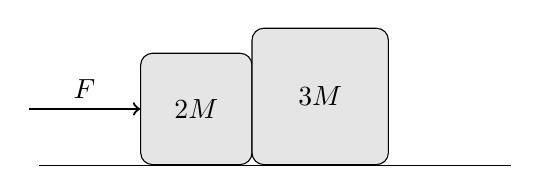
\begin{tikzpicture}
        %% Floor
        \draw (-2,0) -- (4,0);
        %% Mass
        \node[draw,fill=white!90!black,rectangle,rounded corners=1ex,minimum size=1.414cm,anchor=south] (A) at (0,0) {$2M$};
        \node[draw,fill=white!90!black,rectangle,rounded corners=1ex,minimum size=1.732cm,anchor=south] (B) at (1.573,0) {$3M$};
        %% Force
        \draw[thick,<-] (A.west) -- ++(180:1.414) node[pos=0.5,anchor=south] {$F$};
    \end{tikzpicture}
    \end{center}
    If $F=\SI{22}{\newton}$ and $M=\SI{1.0}{\kilo\gram}$ in the figure,
        what is the magnitude of the acceleration of either block?
    \begin{multicols}{3}
    \begin{choices}
        \wrongchoice{\SI{1.8}{\meter\per\second\squared}}
        \wrongchoice{\SI{2.6}{\meter\per\second\squared}}
      \correctchoice{\SI{1.4}{\meter\per\second\squared}}
        \wrongchoice{\SI{2.2}{\meter\per\second\squared}}
        \wrongchoice{\SI{3.7}{\meter\per\second\squared}}
    \end{choices}
    \end{multicols}
\end{question}
}

\element{serway-mc}{
\begin{question}{serway-ch05-q81}
    In the figure, the coefficient of kinetic friction between the surface and the larger block is \num{0.20},
        and the coefficient of kinetic friction between the surface and the smaller block is \num{0.30}. 
    \begin{center}
    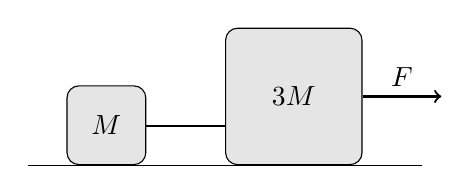
\begin{tikzpicture}
        %% Floor
        \draw (-2,0) -- (3,0);
        %% Mass
        \node[draw,fill=white!90!black,rectangle,rounded corners=1ex,minimum size=1.000cm,anchor=south east] (A) at (-0.5,0) {$M$};
        \node[draw,fill=white!90!black,rectangle,rounded corners=1ex,minimum size=1.732cm,anchor=south west] (B) at (+0.5,0) {$3M$};
        %% Force
        \draw[thick] (A.south east) ++(90:0.5) -- ++(0:1);
        \draw[thick,->] (B.east) -- ++(0:1.0) node[pos=0.5,anchor=south] {$F$};
    \end{tikzpicture}
    \end{center}
    If $F=\SI{14}{\newton}$ and $M=\SI{1.0}{\kilo\gram}$,
        what is the magnitude of the acceleration of either block?
    \begin{multicols}{3}
    \begin{choices}
        \wrongchoice{\SI{2.0}{\meter\per\second\squared}}
      \correctchoice{\SI{1.3}{\meter\per\second\squared}}
        \wrongchoice{\SI{1.5}{\meter\per\second\squared}}
        \wrongchoice{\SI{1.8}{\meter\per\second\squared}}
        \wrongchoice{\SI{3.5}{\meter\per\second\squared}}
    \end{choices}
    \end{multicols}
\end{question}
}

\element{serway-mc}{
\begin{question}{serway-ch05-q82A}
    Two blocks are accelerated across a horizontal frictionless surface as shown.
    Frictional forces keep the two blocks from sliding relative to each other,
        and the two move with the same acceleration. 
    \begin{center}
    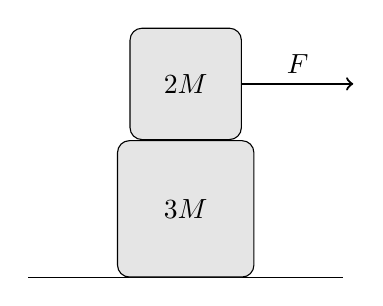
\begin{tikzpicture}
        %% Floor
        \draw (-2,0) -- (2,0);
        %% Mass
        \node[draw,fill=white!90!black,rectangle,rounded corners=1ex,minimum size=1.732cm,anchor=south] (A) at (0,0) {$3M$};
        \node[draw,fill=white!90!black,rectangle,rounded corners=1ex,minimum size=1.414cm,anchor=south] (B) at (A.north) {$2M$};
        %% Force
        \draw[thick,->] (B.east) -- ++(0:1.414) node[pos=0.5,anchor=south] {$F$};
    \end{tikzpicture}
    \end{center}
    If $F=\SI{1.2}{\newton}$ and $M=\SI{1.0}{\kilo\gram}$,
        what is the horizontal component (frictional force)
        of the force of the small block on the large block?
    \begin{multicols}{2}
    \begin{choices}
        \wrongchoice{\SI{0.48}{\newton} to the right}
      \correctchoice{\SI{0.72}{\newton} to the right}
        \wrongchoice{\SI{0.72}{\newton} to the left}
        \wrongchoice{\SI{0.48}{\newton} to the left}
        \wrongchoice{\SI{0.65}{\newton} to the left}
    \end{choices}
    \end{multicols}
\end{question}
}

\element{serway-mc}{
\begin{question}{serway-ch05-q82B}
    Two blocks are accelerated across a horizontal frictionless surface as shown.
    Frictional forces keep the two blocks from sliding relative to each other,
        and the two move with the same acceleration. 
    \begin{center}
    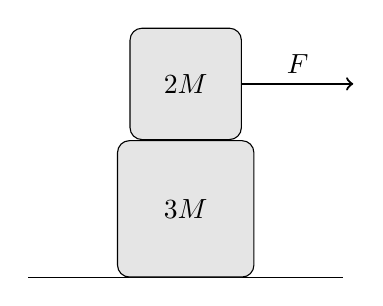
\begin{tikzpicture}
        %% Floor
        \draw (-2,0) -- (2,0);
        %% Mass
        \node[draw,fill=white!90!black,rectangle,rounded corners=1ex,minimum size=1.732cm,anchor=south] (A) at (0,0) {$3M$};
        \node[draw,fill=white!90!black,rectangle,rounded corners=1ex,minimum size=1.414cm,anchor=south] (B) at (A.north) {$2M$};
        %% Force
        \draw[thick,->] (B.east) -- ++(0:1.414) node[pos=0.5,anchor=south] {$F$};
    \end{tikzpicture}
    \end{center}
    If $F=\SI{1.2}{\newton}$ and $M=\SI{1.0}{\kilo\gram}$,
        what is the horizontal component (frictional force)
        of the force of the large block on the small block?
    \begin{multicols}{2}
    \begin{choices}
        \wrongchoice{\SI{0.48}{\newton} to the right}
        \wrongchoice{\SI{0.72}{\newton} to the right}
      \correctchoice{\SI{0.72}{\newton} to the left}
        \wrongchoice{\SI{0.48}{\newton} to the left}
        \wrongchoice{\SI{0.65}{\newton} to the left}
    \end{choices}
    \end{multicols}
\end{question}
}

\element{serway-mc}{
\begin{question}{serway-ch05-q83}
    Two blocks connected by a string are pulled across a horizontal surface by a force applied to one of the blocks,
        as shown. 
    The coefficient of kinetic friction between the blocks and the surface is \num{0.25}. 
    \begin{center}
    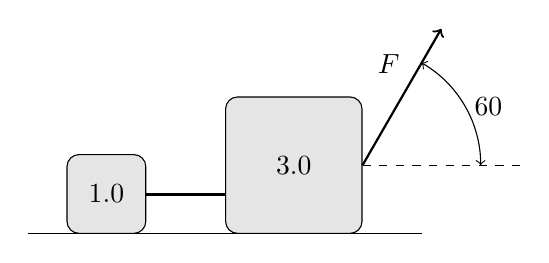
\begin{tikzpicture}
        %% Floor
        \draw (-2,0) -- (3,0);
        %% Mass
        \node[draw,fill=white!90!black,rectangle,rounded corners=1ex,minimum size=1.000cm,anchor=south east] (A) at (-0.5,0) {\SI{1.0}{\kilo\gram}};
        \node[draw,fill=white!90!black,rectangle,rounded corners=1ex,minimum size=1.732cm,anchor=south west] (B) at (+0.5,0) {\SI{3.0}{\kilo\gram}};
        \draw[thick] (A.south east) ++(90:0.5) -- ++(0:1);
        %% Force
        \draw[dashed] (B.east) -- ++(0:2);
        \draw[thick,->] (B.east) -- ++(60:2) node[pos=0.6,anchor=south east] {$F$};
        \draw[<->] (B.east) ++(0:1.5) arc (0:60:1.5) node[pos=0.5,anchor=west] {\ang{60}};
    \end{tikzpicture}
    \end{center}
    If each block has an acceleration of \SI{2.0}{\meter\per\second\squared} to the right,
        what is the magnitude $F$ of the applied force?
    \begin{multicols}{3}
    \begin{choices}
      \correctchoice{\SI{25}{\newton}}
        \wrongchoice{\SI{18}{\newton}}
        \wrongchoice{\SI{11}{\newton}}
        \wrongchoice{\SI{14}{\newton}}
        \wrongchoice{\SI{7.0}{\newton}}
    \end{choices}
    \end{multicols}
\end{question}
}

\element{serway-mc}{
\begin{question}{serway-ch05-q84}
    In the figure,
        the coefficient of kinetic friction between the surface and the larger block is \num{0.20},
        and the coefficient of kinetic friction between the surface and the smaller block is \num{0.30}. 
    \begin{center}
    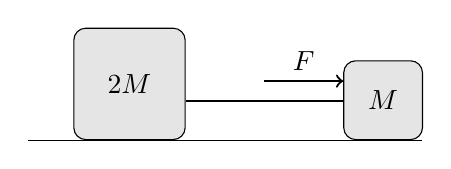
\begin{tikzpicture}
        %% Floor
        \draw (-3,0) -- (2,0);
        %% Mass
        \node[draw,fill=white!90!black,rectangle,rounded corners=1ex,minimum size=1.414cm,anchor=south east] (A) at (-1.00,0) {$2M$};
        \node[draw,fill=white!90!black,rectangle,rounded corners=1ex,minimum size=1.000cm,anchor=south west] (B) at (+1.00,0) {$M$};
        \draw[thick] (A.south east) ++(90:0.5) -- ++(0:2.0);
        %% Force
        \draw[thick,<-] (B.south west) ++ (90:0.75) -- ++(180:1) node[pos=0.5,anchor=south] {$F$};
    \end{tikzpicture}
    \end{center}
    If $F=\SI{10}{\newton}$ and $M=\SI{1.0}{\kilo\gram}$,
        what is the tension in the connecting string?
    \begin{multicols}{3}
    \begin{choices}
        \wrongchoice{\SI{8.0}{\newton}}
      \correctchoice{\SI{6.0}{\newton}}
        \wrongchoice{\SI{6.7}{\newton}}
        \wrongchoice{\SI{8.7}{\newton}}
        \wrongchoice{\SI{3.0}{\newton}}
    \end{choices}
    \end{multicols}
\end{question}
}

\element{serway-mc}{
\begin{question}{serway-ch05-q85}
    The frictional force of the floor on a large suitcase is least when the suitcase is:
    \begin{choices}
        \wrongchoice{pushed by a force parallel to the floor.}
        \wrongchoice{dragged by a force parallel to the floor.}
      \correctchoice{pulled by a force directed at an angle $\theta$ above the floor.}
        \wrongchoice{pushed by a force directed at an angle $\theta$ into the floor.}
        \wrongchoice{turned on its side and pushed by a force parallel to the floor.}
    \end{choices}
\end{question}
}

\element{serway-mc}{
\begin{question}{serway-ch05-q86}
    A \SI{60}{\kilo\gram} person rides down an icy hill of \ang{20} slope while standing on a \SI{3.0}{\kilo\gram} flat-bottomed bathroom scale. 
    Assume there is no frictional force between the bottom of the scale and the hill. 
    The static friction force the scale exerts on the person is:
    \begin{multicols}{3}
    \begin{choices}
      \correctchoice{\SI{0}{\newton}.}
        \wrongchoice{\SI{201}{\newton}.}
        \wrongchoice{\SI{211}{\newton}.}
        \wrongchoice{\SI{553}{\newton}.}
        \wrongchoice{\SI{580}{\newton}.}
    \end{choices}
    \end{multicols}
\end{question}
}

\element{serway-mc}{
\begin{question}{serway-ch05-q87}
    A chair is placed on a rug. 
    Then a book is placed on the chair. 
    The floor exerts a normal force:
    \begin{choices}
        \wrongchoice{on all three.}
        \wrongchoice{only on the book.}
        \wrongchoice{only on the rug.}
      \correctchoice{upwards on the rug and downwards on the chair.}
        \wrongchoice{only on the objects you have defined to be part of the system.}
    \end{choices}
\end{question}
}

\newcommand{\serwayChFiveQEightEight}{
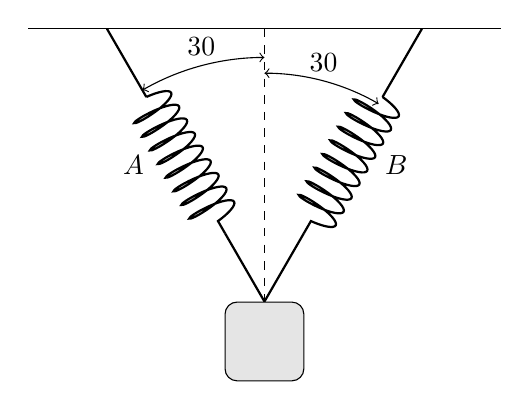
\begin{tikzpicture}
    %% Nodes
    \coordinate (A) at (-2,0);
    \coordinate (B) at (+2,0);
    \coordinate (C) at (0,-3.464);
    %% Ceiling
    \draw (-3,0) -- (3,0);
    %% Springs
    \draw[thick] (A) -- ++(300:1);
    \draw[thick,decoration={aspect=0.2,segment length=2.0mm,amplitude=3mm,coil},decorate]
        (A) ++(300:1) -- ++(300:2) node[pos=0.5,anchor=east,xshift=-4mm] {$A$};
    \draw[thick] (A) ++(300:3) --(C);
    \draw[thick] (B) -- ++(240:1);
    \draw[thick,decoration={aspect=0.2,segment length=2.0mm,amplitude=3mm,coil},decorate]
        (B) ++(240:1) -- ++(240:2) node[pos=0.5,anchor=west,xshift=4mm] {$B$};
    \draw[thick] (B) ++(240:3) --(C);
    \draw[dashed] (0,0) -- (C);
    %% Angles
    \draw[<->] (C) ++(60:2.9) arc(60:90:2.9) node[pos=0.5,anchor=south] {\ang{30}};
    \draw[<->] (C) ++(120:3.1) arc(120:90:3.1) node[pos=0.5,anchor=south] {\ang{30}};
    %\draw[<->] (C) ++ (90:2) arc (90:130:2cm) node[pos=0.5,anchor=south] {\ang{40}};
    %% Mass
    \node[draw,fill=white!90!black,rectangle,rounded corners=1ex,minimum size=1cm,anchor=north] (M) at (C) {};
\end{tikzpicture}
}

\element{serway-mc}{
\begin{question}{serway-ch05-q88}
    Two identical springs with spring constant \SI{50}{\newton\per\meter} support a \SI{5.0}{\newton} weight as in the picture below. 
    \begin{center}
        \serwayChFiveQEightEight
    \end{center}
    What is the tension in spring A?  
    \begin{multicols}{3}
    \begin{choices}
        \wrongchoice{\SI{1.45}{\newton}}
        \wrongchoice{\SI{2.50}{\newton}}
      \correctchoice{\SI{2.89}{\newton}}
        \wrongchoice{\SI{3.75}{\newton}}
        \wrongchoice{\SI{5.00}{\newton}}
    \end{choices}
    \end{multicols}
\end{question}
}

\element{serway-mc}{
\begin{question}{serway-ch05-q89}
    Two identical springs with spring constant \SI{50}{\newton\per\meter} support a \SI{5.0}{\newton} weight as in the picture below. 
    \begin{center}
        \serwayChFiveQEightEight
    \end{center}
    What is the change in length of each spring when the weight is hung on the springs.?
    \begin{multicols}{3}
    \begin{choices}
        \wrongchoice{\SI{2.9}{\centi\meter}}
        \wrongchoice{\SI{5.0}{\centi\meter}}
      \correctchoice{\SI{5.8}{\centi\meter}}
        \wrongchoice{\SI{7.5}{\centi\meter}}
        \wrongchoice{\SI{10.0}{\centi\meter}}
    \end{choices}
    \end{multicols}
\end{question}
}

\element{serway-mc}{
\begin{question}{serway-ch05-q90}
    A book is placed on a chair. 
    Then a videocassette is placed on the book. 
    The floor exerts a normal force:
    \begin{choices}
        \wrongchoice{on all three.}
        \wrongchoice{only on the book.}
      \correctchoice{only on the chair.}
        \wrongchoice{upwards on the chair and downwards on the book.}
        \wrongchoice{only on the objects that you have defined to be part of the system.}
    \end{choices}
\end{question}
}

\element{serway-mc}{
\begin{question}{serway-ch05-q91}
    Two bodies, $A$ and $B$, collide as shown in Figures (a) and (b) below.
    \begin{center}
    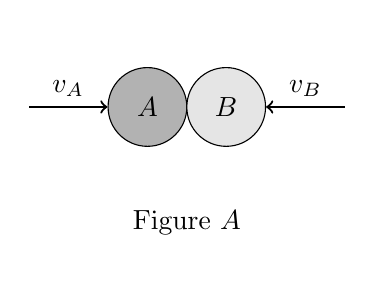
\begin{tikzpicture}
        \draw[white] (-1.75,-2) rectangle (2,1);
        \node[fill=white!70!black,draw,circle,minimum size=1cm,anchor=center] (A) at (-0.5,0) {$A$};
        \draw[thick,<-] (A.west) -- ++(180:1) node[pos=0.5,anchor=south] {$v_A$};
        \node[fill=white!90!black,draw,circle,minimum size=1cm,anchor=center] (B) at (+0.5,0) {$B$};
        \draw[thick,<-] (B.east) -- ++(0:1) node[pos=0.5,anchor=south] {$v_B$};
        \node[anchor=south] at (0,-1.75) {Figure $A$};
    \end{tikzpicture}
    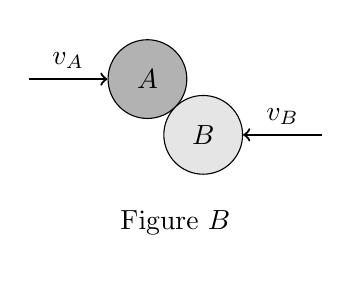
\begin{tikzpicture}
        \draw[white] (-1.75,-2) rectangle (2,1);
        \node[fill=white!70!black,draw,circle,minimum size=1cm,anchor=center] (A) at (-0.354,+0.354) {$A$};
        \draw[thick,<-] (A.west) -- ++(180:1) node[pos=0.5,anchor=south] {$v_A$};
        \node[fill=white!90!black,draw,circle,minimum size=1cm,anchor=center] (B) at (+0.354,-0.354) {$B$};
        \draw[thick,<-] (B.east) -- ++(0:1) node[pos=0.5,anchor=south] {$v_B$};
        \node[anchor=south] at (0,-1.75) {Figure $B$};
    \end{tikzpicture}
    \end{center}
    Which statement is true?
    \begin{choices}
        \wrongchoice{They exert equal and opposite forces on each other in (a) but not in (b).}
        \wrongchoice{They exert equal and opposite force on each other in (b) but not in (a).}
      \correctchoice{They exert equal and opposite force on each other in both (a) and (b).}
        \wrongchoice{The forces are equal and opposite to each other in (a), but only the components of the forces parallel to the velocities are equal in (b).}
        \wrongchoice{The forces are equal and opposite in (a), but only the components of the forces perpendicular to the velocities are equal in (b).}
    \end{choices}
\end{question}
}

\element{serway-mc}{
\begin{question}{serway-ch05-q92}
    You throw a ball up in the air and hold your hand under it to catch it when it comes down. 
    The reason why the ball stops is because:
    \begin{choices}
        \wrongchoice{your hand is there: your hand exerts no force on the ball.}
        \wrongchoice{your hand exerts a force on the ball perpendicular to its velocity.}
        \wrongchoice{your hand exerts a force on the ball in the direction of its velocity.}
      \correctchoice{your hand exerts a force on the ball in the direction opposite to its velocity.}
        \wrongchoice{your hand and the ball exert forces in the same direction on each other.}
    \end{choices}
\end{question}
}

\element{serway-mc}{
\begin{question}{serway-ch05-q93}
    You hold a tennis racket in your hand. 
    On top of the racket you have balanced a ball. 
    Which statement is true?
    \begin{choices}
        \wrongchoice{The force of your hand on the racket and the force of the ball on the racket are equal and opposite.}
        \wrongchoice{The force of the racket on your hand and the force of the ball on the racket are equal and opposite.}
        \wrongchoice{The force of your hand on the racket and the force of the racket on the ball are equal and opposite.}
        \wrongchoice{The force of the racket on your hand and the force of the racket on the ball are equal and opposite.}
      \correctchoice{The force of your hand on the racket and the force of the racket on your hand are equal and opposite.}
    \end{choices}
\end{question}
}

\element{serway-mc}{
\begin{question}{serway-ch05-q94}
    When you drag a toy teddy bear along the floor by a force that is parallel to the floor,
        the magnitude of the force of friction:
    \begin{choices}
      \correctchoice{is independent of velocity or acceleration.}
        \wrongchoice{increases when the velocity increases.}
        \wrongchoice{is proportional to the acceleration.}
        \wrongchoice{decreases when the force parallel to the floor increases.}
        \wrongchoice{increases when the force parallel to the floor increases.}
    \end{choices}
\end{question}
}

\element{serway-mc}{
\begin{question}{serway-ch05-q95}
    In order to jump off the floor,
        the floor must exert a force on you:
    \begin{choices}
        \wrongchoice{in the direction of and equal to your weight.}
        \wrongchoice{opposite to and equal to your weight.}
        \wrongchoice{in the direction of and less than your weight.}
        \wrongchoice{opposite to and less than your weight.}
      \correctchoice{opposite to and greater than your weight.}
    \end{choices}
\end{question}
}

\element{serway-mc}{
\begin{question}{serway-ch05-q96}
    When an acrobat hangs motionless from a pair of rings:
    \begin{choices}
        \wrongchoice{she has no measurable weight.}
        \wrongchoice{her weight depends on the angles the ropes make with the ceiling.}
        \wrongchoice{her weight is reduced by the upward force the rings exert on her.}
        \wrongchoice{her weight is increased by the upward force the rings exert on her.}
      \correctchoice{she exerts a gravitational force on the Earth that is equal to the sum of the forces the rings exert on her.}
    \end{choices}
\end{question}
}

\element{serway-mc}{
\begin{question}{serway-ch05-q97}
    Three boxes slide on a frictionless horizontal surface when pulled by a force of magnitude $F$. 
    \begin{center}
    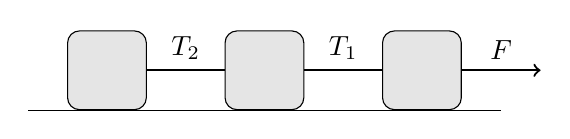
\begin{tikzpicture}
        %% Floor
        \draw (-1,0) -- (5,0);
        %% Mass
        \node[draw,fill=white!90!black,rectangle,rounded corners=1ex,minimum size=1cm,anchor=south] (A) at (0,0) {};
        \node[draw,fill=white!90!black,rectangle,rounded corners=1ex,minimum size=1cm,anchor=south] (B) at (2,0) {};
        \node[draw,fill=white!90!black,rectangle,rounded corners=1ex,minimum size=1cm,anchor=south] (C) at (4,0) {};
        %% Rope
        \draw[thick] (A.east) -- (B.west) node[pos=0.5,anchor=south] {$T_2$};
        \draw[thick] (B.east) -- (C.west) node[pos=0.5,anchor=south] {$T_1$};
        \draw[thick,->] (C.east) -- ++(0:1) node[pos=0.5,anchor=south] {$F$};
    \end{tikzpicture}
    \end{center}
    When we compare the tensions $T_1$ and $T_2$ with the force $F$, we find that:
    \begin{multicols}{2}
    \begin{choices}
        \wrongchoice{$T_1 = T_2 = F$.}
        \wrongchoice{$T_1 = F > T_2$.}
        \wrongchoice{$F > T_1 = T_2$.}
      \correctchoice{$F > T_1 > T_2$.}
        %% NOTE: parenthesis ?
        \wrongchoice{$F - T_1 < T_1 - T_2$.}
    \end{choices}
    \end{multicols}
\end{question}
}

\element{serway-mc}{
\begin{question}{serway-ch05-q98}
    Three boxes are pushed across a frictionless horizontal surface as shown. 
    \begin{center}
    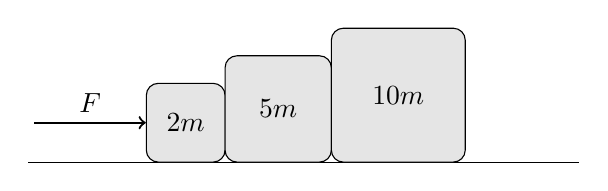
\begin{tikzpicture}
        %% Floor
        \draw (-2,0) -- (5,0);
        %% Mass
        \node[draw,fill=white!90!black,rectangle,rounded corners=1ex,minimum size=1.00cm,anchor=south] (A) at (0,0) {$2m$};
        \node[draw,fill=white!90!black,rectangle,rounded corners=1ex,minimum size=1.35cm,anchor=south] (B) at (1.175,0) {$5m$};
        \node[draw,fill=white!90!black,rectangle,rounded corners=1ex,minimum size=1.70cm,anchor=south] (C) at (2.70,0) {$10m$};
        %% Force
        \draw[thick,<-] (A.west) -- ++(180:1.414) node[pos=0.5,anchor=south] {$F$};
    \end{tikzpicture}
    \end{center}
    When we compare the normal force $N_{2,5}$ that mass $2m$ exerts on mass $5m$ with the normal force $N_{5,10}$ that mass $5m$ exerts on mass $10m$,
        we find that:
    \begin{multicols}{2}
    \begin{choices}
        \wrongchoice{$N_{2,5} = N_{5,10} = F$.}
        \wrongchoice{$N_{2,5} = F > N_{5,10}$.}
        \wrongchoice{$F > N_{2,5} = N_{5,10}$.}
      \correctchoice{$F > N_{2,5} > N_{5,10}$.}
        \wrongchoice{$F > N_{5,10} > N_{2,5}$.}
    \end{choices}
    \end{multicols}
\end{question}
}

\element{serway-mc}{
\begin{questionmult}{serway-ch05-q99}
    Given the equation 
    \begin{equation*}
        \left( \SI{2.00}{\kilo\gram} \right) \left( \SI{5.00}{\meter\per\second\squared} \right) = \SI{20.00}{\newton} - \SI{10.00}{\newton}, 
    \end{equation*}
    which answer or answers provides(s) the best description of a possible physical situation?
    \begin{choices}
      \correctchoice{A \SI{20.00}{\newton} tension pulls a \SI{2.00}{\kilo\gram} mass.  The \SI{2.00}{\kilo\gram} mass pulls another \SI{2.00}{\kilo\gram} mass.}
      \correctchoice{A \SI{20.00}{\newton} tension pushes a \SI{2.00}{\kilo\gram} mass.  The \SI{2.00}{\kilo\gram} mass pushes another \SI{2.00}{\kilo\gram} mass.}
        \wrongchoice{A \SI{2.00}{\kilo\gram} mass on a flat surface is acted on by gravity while another \SI{2.00}{\kilo\gram} mass sits on top of it.}
        %\wrongchoice{All of the situations above are possible.}
      %\correctchoice{Only (a) and (b) above are possible.}
    \end{choices}
\end{questionmult}
}

\element{serway-mc}{
\begin{question}{serway-ch05-q100}
    Given the equation 
    \begin{align*}
        \left(\SI{3.00}{\kilo\gram}\right) \left(\SI{5.88}{\meter\per\second\squared}\right) &=
        \left(\SI{3.00}{\kilo\gram}\right) \left(\SI{9.80}{\meter\per\second\squared}\right) \\
        &-\left(\SI{2.00}{\kilo\gram}\right) \left(\SI{5.88}{\meter\per\second\squared}\right) \\
    \end{align*}
    which answer or answers provides(s) the best description of a possible physical situation?
    \begin{choices}
        \wrongchoice{A \SI{3.00}{\kilo\gram} mass is suspended from the ceiling.}
        \wrongchoice{A \SI{2.00}{\kilo\gram} mass hanging over a pulley drags a \SI{3.00}{\kilo\gram} mass along a frictionless horizontal surface.}
      \correctchoice{A \SI{3.00}{\kilo\gram} mass hanging over a pulley drags a \SI{2.00}{\kilo\gram} mass along a frictionless horizontal surface.}
        \wrongchoice{A \SI{3.00}{\kilo\gram} mass hanging over a pulley drags a \SI{5.00}{\kilo\gram} mass along a frictionless horizontal surface.}
        \wrongchoice{A \SI{5.00}{\kilo\gram} mass hanging over a pulley drags a \SI{3.00}{\kilo\gram} mass along a frictionless horizontal surface.}
    \end{choices}
\end{question}
}

\element{serway-mc}{
\begin{question}{serway-ch05-q101}
    Two experiments are performed. 
    In (A), an \SI{18.0}{\newton} force pushes horizontally on a \SI{2.00}{\kilo\gram} block that then pushes on a \SI{4.00}{\kilo\gram} block. 
    In (B), an \SI{18.0}{\newton} force pushes on a \SI{4.00}{\kilo\gram} block that then pushes on a \SI{2.00}{\kilo\gram} block. 
    Which statement is correct?
    \begin{choices}
      \correctchoice{The acceleration is \SI{3.00}{\meter\per\second\squared} in both (A) and (B).}
        \wrongchoice{The acceleration is \SI{4.50}{\meter\per\second\squared} in both (A) and (B).}
        \wrongchoice{The acceleration is \SI{6.00}{\meter\per\second\squared} in both (A) and (B).}
        \wrongchoice{The acceleration is \SI{9.00}{\meter\per\second\squared} in both (A) and (B).}
        \wrongchoice{The \SI{2.00}{\kilo\gram} block has a \SI{9.00}{\meter\per\second\squared} acceleration. 
            The \SI{4.00}{\kilo\gram} block has a \SI{4.50}{\meter\per\second\squared} acceleration.}
    \end{choices}
\end{question}
}

\element{serway-mc}{
\begin{question}{serway-ch05-q102}
    A catcher arranges to catch a baseball dropped from a height \SI{50}{\meter} above his glove. 
    However, his friends substitute a soft \SI{250}{\gram} red grapefruit,
        so that it will smash apart when he catches it. 
    His glove stops the grapefruit in \SI{0.010}{\second}. 
    What force does the glove exert on the grapefruit?
    \begin{multicols}{2}
    \begin{choices}
        \wrongchoice{\SI{0.0783}{\newton}}
      \correctchoice{\SI{783}{\newton}}
        \wrongchoice{\SI{2 450}{\newton}}
        \wrongchoice{\SI{24 500}{\newton}}
        \wrongchoice{\SI{78 300}{\newton}}
    \end{choices}
    \end{multicols}
\end{question}
}

\element{serway-mc}{
\begin{question}{serway-ch05-q103}
    Jean is moving two boxes down the hall towards her dorm room. 
    The smaller box, of \SI{80}{\newton} weight, is in front of the larger box, of \SI{160}{\newton} weight. 
    She finds that she is pushing on the larger box with an \SI{84}{\newton} force. 
    Jimmy tells her that means that she is also pushing on the smaller box with an \SI{84}{\newton} force. 
    Clara tells Jimmy that he is wrong,
        because the force is divided between the two boxes in proportion to their weights as long as they have equal coefficients of kinetic friction. 
    Which one, if either, is correct, Clara or Jimmy?
    \begin{choices}
        \wrongchoice{Jimmy is correct because the larger box transmits the force to the smaller box.}
        \wrongchoice{Jimmy is correct because Jean is pushing the larger box and the 84 N force pushes the smaller box.}
      \correctchoice{Clara is correct because the applied force pushes the total mass of both boxes.}
        \wrongchoice{Clara is correct because an applied force on one of any two bodies always acts on the bodies in a 2:1 ratio.}
        \wrongchoice{Neither is correct because we cannot calculate the forces on the individual boxes.}
    \end{choices}
\end{question}
}

\newcommand{\serwayChfiveQOneZeroFour}{
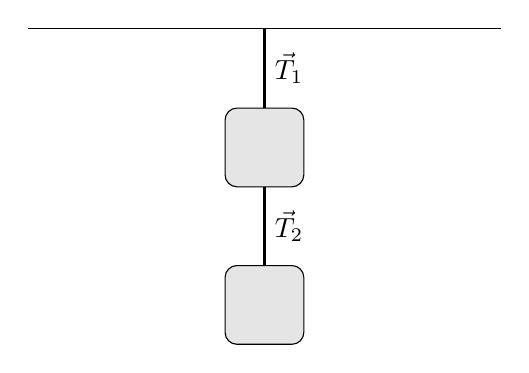
\begin{tikzpicture}
    %% Ceiling
    \draw (-3,0) -- (+3,0);
    %% Masses
    \node[draw,fill=white!90!black,rectangle,rounded corners=1ex,minimum size=1cm,anchor=north] (A) at (0,-1.0) {};
    \node[draw,fill=white!90!black,rectangle,rounded corners=1ex,minimum size=1cm,anchor=north] (B) at (0,-3.0) {};
    %% String
    \draw[thick] (0,0)  -- (A.north) node[pos=0.5,anchor=west] {$\vec{T}_1$};
    \draw[thick] (A.south)  -- (B.north) node[pos=0.5,anchor=west] {$\vec{T}_2$};
\end{tikzpicture}
}


\element{serway-mc}{
\begin{question}{serway-ch05-q104}
    A \SI{2.30}{\kilo\gram} mass is suspended from the ceiling and a \SI{1.70}{\kilo\gram} mass is suspended from the \SI{2.30}{\kilo\gram} mass, as shown. 
    \begin{center}
        \serwayChfiveQOneZeroFour
    \end{center}
    The tensions in the strings are labeled $T_1$ and $T_2$.
    A hand exerts an upward force of \SI{6.70}{\newton} on the \SI{1.70}{\kilo\gram} mass. 
    The magnitudes of the tensions are:
    %\begin{multicols}{2}
    \begin{choices}
        \wrongchoice{$T_1 = \SI{15.8}{\newton}$; $T_2 = \SI{10.0}{\newton}$.}
        \wrongchoice{$T_1 = \SI{15.8}{\newton}$; $T_2 = \SI{16.7}{\newton}$.}
        \wrongchoice{$T_1 = \SI{22.5}{\newton}$; $T_2 = \SI{10.0}{\newton}$.}
        \wrongchoice{$T_1 = \SI{22.5}{\newton}$; $T_2 = \SI{16.7}{\newton}$.}
      \correctchoice{$T_1 = \SI{32.5}{\newton}$; $T_2 = \SI{10.0}{\newton}$.}
    \end{choices}
    %\end{multicols}
\end{question}
}

\element{serway-mc}{
\begin{question}{serway-ch05-q105}
    A \SI{2.30}{\kilo\gram} mass is suspended from the ceiling and a \SI{1.70}{\kilo\gram} mass is suspended from the \SI{2.30}{\kilo\gram} mass, as shown. 
    \begin{center}
        \serwayChfiveQOneZeroFour
    \end{center}
    The tensions in the strings are labeled $T_1$ and $T_2$. 
    The string supporting the \SI{1.70}{\kilo\gram} mass is cut. 
    The magnitudes of the tension in string 1 before and after string 2 is cut are:
    %\begin{multicols}{2}
    \begin{choices}
        \wrongchoice{$T_{1,i} = \SI{22.5}{\newton}$; $T_{1,f} = \SI{5.80}{\newton}$.}
        \wrongchoice{$T_{1,i} = \SI{39.2}{\newton}$; $T_{1,f} = \SI{5.80}{\newton}$.}
        \wrongchoice{$T_{1,i} = \SI{22.5}{\newton}$; $T_{1,f} = \SI{22.5}{\newton}$.}
      \correctchoice{$T_{1,i} = \SI{39.2}{\newton}$; $T_{1,f} = \SI{22.5}{\newton}$.}
        \wrongchoice{$T_{1,i} = \SI{39.2}{\newton}$; $T_{1,f} = \SI{39.2}{\newton}$.}
    \end{choices}
    %\end{multicols}
\end{question}
}

\element{serway-mc}{
\begin{question}{serway-ch05-q106}
    A \SI{6.00}{\kilo\gram} block is placed on a \ang{30.0} incline and connected to another block on a \ang{36.87} incline. 
    \begin{center}
    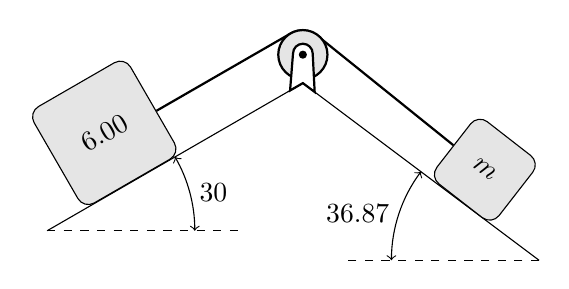
\begin{tikzpicture}[scale=1.25]
        %% Floor
        \draw (0,0) -- (323.13:3);
        \draw (0,0) -- ++(210:3);
        %% Angles
        \draw[dashed] (0,0) ++ (323.13:3) -- ++(180:2);
        \draw[<->] (0,0) ++ (323.13:3) ++(180:1.5) arc(180:143.13:1.5) node[anchor=east,pos=0.5] {\ang{36.87}};
        \draw[dashed] (0,0) ++ (210:3) -- ++(0:2);
        \draw[<->] (0,0) ++ (210:3) ++(0:1.5) arc(0:30:1.5) node[anchor=west,pos=0.5] {\ang{30}};
        %% Mass
        \node[draw,fill=white!90!black,rectangle,rounded corners=1ex,minimum size=1.414cm,anchor=south,rotate=30] (A) at (210:2) {\SI{6.00}{\kilo\gram}};
        \node[draw,fill=white!90!black,rectangle,rounded corners=1ex,minimum size=1.0cm,anchor=south,rotate=-37.87] (B) at (323.13:2) {$m$};
        %% Rope and Pully
        %% (-r sin\theta, r*tan*sin) and (0, (h-r)/cos\theta)
        \draw[thick] (A.south east) ++(120:0.50) -- (-0.125,0.504) arc(120:53.13:0.24) -- (B.west);
        \draw[thick,fill=white!90!black] (0,0.289) circle (0.25); 
        \draw[thick,fill=white] (210:0.15) -- (-0.1,0.3) arc (180:0:0.1) -- (323.13:0.15) -- (0,0) -- cycle;
        \draw[fill] (0,0.289) circle (1pt);
    \end{tikzpicture}
    \end{center}
    Although the surfaces are frictionless the blocks do not move.
    What is the mass in kilograms of the block on the \ang{36.87} incline?
    \begin{multicols}{3}
    \begin{choices}
        \wrongchoice{\SI{1.80}{\kilo\gram}}
        \wrongchoice{\SI{3.00}{\kilo\gram}}
        \wrongchoice{\SI{4.00}{\kilo\gram}}
      \correctchoice{\SI{5.00}{\kilo\gram}}
        \wrongchoice{\SI{6.00}{\kilo\gram}}
    \end{choices}
    \end{multicols}
\end{question}
}

\element{serway-mc}{
\begin{question}{serway-ch05-q107}
    A \SI{4.00}{\kilo\gram} block is suspended from the roof of an elevator. 
    A \SI{2.00}{\kilo\gram} block is suspended from the \SI{4.00}{\kilo\gram} block. 
    The tensions in strings 1 and 2 are labeled $T_1$ and $T_2$.
    \begin{center}
        \serwayChfiveQOneZeroFour
    \end{center}
    When the elevator a ccelerates upwards with an acceleration of \SI{2.20}{\meter\per\second\squared},
        the magnitudes of $T_1$ and $T_2$ are
    \begin{multicols}{2}
    \begin{choices}
        \wrongchoice{\SI{30.4}{\newton}; \SI{15.2}{\newton}.}
        \wrongchoice{\SI{39.2}{\newton}; \SI{19.6}{\newton}.}
        \wrongchoice{\SI{45.6}{\newton}; \SI{15.2}{\newton}.}
        \wrongchoice{\SI{48.0}{\newton}; \SI{24.0}{\newton}.}
      \correctchoice{\SI{72.0}{\newton}; \SI{24.0}{\newton}.}
    \end{choices}
    \end{multicols}
\end{question}
}

\element{serway-mc}{
\begin{question}{serway-ch05-q108}
    A \SI{4.00}{\kilo\gram} block is suspended from the roof of an elevator. 
    A \SI{2.00}{\kilo\gram} block is suspended from the \SI{4.00}{\kilo\gram} block. 
    The tensions in strings 1 and 2 are labeled $T_1$ and $T_2$.
    \begin{center}
        \serwayChfiveQOneZeroFour
    \end{center}
    The tensions in strings 1 and 2 are labeled $T_1$ and $T_2$.
    When the elevator accelerates downwards with an acceleration of \SI{2.20}{\meter\per\second\squared},
        the magnitudes of $T_1$ and $T_2$ are:
    \begin{multicols}{2}
    \begin{choices}
        \wrongchoice{\SI{30.4}{\newton}; \SI{15.2}{\newton}.}
      \correctchoice{\SI{39.2}{\newton}; \SI{19.6}{\newton}.}
        \wrongchoice{\SI{45.6}{\newton}; \SI{15.2}{\newton}.}
        \wrongchoice{\SI{48.0}{\newton}; \SI{24.0}{\newton}.}
        \wrongchoice{\SI{72.0}{\newton}; \SI{24.0}{\newton}.}
    \end{choices}
    \end{multicols}
\end{question}
}

\element{serway-mc}{
\begin{question}{serway-ch05-q109}
    Aline and Charlie are arguing as to whether or not it is possible in principle
        for an elevator to have an acceleration of magnitude greater than $g$. 
    In the course of their discussion they come up with the statements below. 
    Which one is correct?
    \begin{choices}
        \wrongchoice{No, because once $|\mathbf{a}|$ reaches $g$, the elevator is in free fall.}
        \wrongchoice{No, because an acceleration greater than $g$ is not possible.}
        \wrongchoice{Yes because it can reach an acceleration greater than $g$ when the cable breaks.}
      \correctchoice{Yes, because it can reach an acceleration greater than $g$ if the motor is strong enough.}
        \wrongchoice{No, because it cannot exceed its terminal acceleration.}
    \end{choices}
\end{question}
}


\endinput




%%--------------------------------------------------
%% Serway: Physics for Scientists and Engineers
%%--------------------------------------------------


%% Chapter 06: Circular Motion and other
%%     Applications of Newton's Laws
%%--------------------------------------------------


%% Table of Contents
%%--------------------------------------------------

%% 6.1 Newton's Second Law for a Particle in Uniform Circular Motion
%% 6.2 Nonuniform Circular Motion
%% 6.3 Motion in Accelerated Frames
%% 6.4 Motion in the Presence of Resistive Forces


%% Serway Multiple Choice Questions
%%--------------------------------------------------
\element{serway-mc}{
\begin{question}{serway-ch06-q01}
    A race car travels \SI{40}{\meter\per\second} around a banked (\ang{45} with the horizontal)
        circular (radius = \SI{0.20}{\kilo\meter}) track. 
    What is the magnitude of the resultant force on the \SI{80}{\kilo\gram} driver of this car?
    \begin{multicols}{3}
    \begin{choices}
        \wrongchoice{\SI{0.68}{\kilo\newton}}
      \correctchoice{\SI{0.64}{\kilo\newton}}
        \wrongchoice{\SI{0.72}{\kilo\newton}}
        \wrongchoice{\SI{0.76}{\kilo\newton}}
        \wrongchoice{\SI{0.52}{\kilo\newton}}
    \end{choices}
    \end{multicols}
\end{question}
}

\element{serway-mc}{
\begin{question}{serway-ch06-q02}
    An airplane travels \SI{80}{\meter\per\second} as it makes a horizontal
        circular turn which has a \SI{0.80}{\kilo\meter} radius. 
    What is the magnitude of the resultant force on the
        \SI{75}{\kilo\gram} pilot of this airplane?
    \begin{multicols}{3}
    \begin{choices}
        \wrongchoice{\SI{0.69}{\kilo\newton}}
        \wrongchoice{\SI{0.63}{\kilo\newton}}
        \wrongchoice{\SI{0.66}{\kilo\newton}}
      \correctchoice{\SI{0.60}{\kilo\newton}}
        \wrongchoice{\SI{0.57}{\kilo\newton}}
    \end{choices}
    \end{multicols}
\end{question}
}

\element{serway-mc}{
\begin{question}{serway-ch06-q03}
    An airplane moves \SI{140}{\meter\per\second} as it travels around a vertical circular loop which has a \SI{1.0}{\kilo\meter} radius. 
    What is the magnitude of the resultant force on the \SI{70}{\kilo\gram} pilot of this plane at the bottom of this loop?
    \begin{multicols}{3}
    \begin{choices}
        \wrongchoice{\SI{2.1}{\kilo\newton}}
      \correctchoice{\SI{1.4}{\kilo\newton}}
        \wrongchoice{\SI{0.69}{\kilo\newton}}
        \wrongchoice{\SI{1.5}{\kilo\newton}}
        \wrongchoice{\SI{1.3}{\kilo\newton}}
    \end{choices}
    \end{multicols}
\end{question}
}

\element{serway-mc}{
\begin{question}{serway-ch06-q04}
    A car travels along the perimeter of a vertical circle
        (radius = \SI{0.25}{\kilo\meter}) at a constant speed of \SI{30}{\meter\per\second}. 
    What is the magnitude of the resultant force on the \SI{60}{\kilo\gram}
        driver of the car at the lowest point on this circular path?
    \begin{multicols}{3}
    \begin{choices}
        \wrongchoice{\SI{0.37}{\kilo\newton}}
        \wrongchoice{\SI{0.80}{\kilo\newton}}
      \correctchoice{\SI{0.22}{\kilo\newton}}
        \wrongchoice{\SI{0.59}{\kilo\newton}}
        \wrongchoice{\SI{0.45}{\kilo\newton}}
    \end{choices}
    \end{multicols}
\end{question}
}

\element{serway-mc}{
\begin{question}{serway-ch06-q05}
    A \SI{30}{\kilo\gram} child rides on a circus Ferris wheel that takes her
        around a vertical circular path with a radius of \SI{20}{\meter} every \SI{22}{\second}.
    What is the magnitude of the resultant force on the child at the highest point on this trajectory?
    \begin{multicols}{3}
    \begin{choices}
      \correctchoice{\SI{49}{\newton}}
        \wrongchoice{\SI{0.29}{\kilo\newton}}
        \wrongchoice{\SI{0.34}{\kilo\newton}}
        \wrongchoice{\SI{0.25}{\kilo\newton}}
        \wrongchoice{\SI{0.76}{\kilo\newton}}
    \end{choices}
    \end{multicols}
\end{question}
}

\element{serway-mc}{
\begin{question}{serway-ch06-q06}
    An amusement ride consists of a car moving in a vertical circle on the end of a rigid boom. 
    The radius of the circle is \SI{10}{\meter}. 
    The combined weight of the car and riders is \SI{5.0}{\kilo\newton}.
    At the top of the circle the car has a speed of \SI{5.0}{\meter\per\second}
        which is not changing at that instant. 
    What is the force of the boom on the car at the top of the circle?
    \begin{multicols}{2}
    \begin{choices}
        \wrongchoice{\SI{3.7}{\kilo\newton} (Down)}
        \wrongchoice{\SI{1.3}{\kilo\newton} (Down)}
        \wrongchoice{\SI{6.3}{\kilo\newton} (Up)}
      \correctchoice{\SI{3.7}{\kilo\newton} (Up)}
        \wrongchoice{\SI{5.2}{\kilo\newton} (Down)}
    \end{choices}
    \end{multicols}
\end{question}
}

\element{serway-mc}{
\begin{question}{serway-ch06-q07}
    A highway curve has a radius of \SI{0.14}{\kilo\meter} and is unbanked. 
    A car weighing \SI{12}{\kilo\newton} goes around the curve at a speed of \SI{24}{\meter\per\second} without slipping. 
    What is the magnitude of the horizontal force of the road on the car?
    \begin{multicols}{3}
    \begin{choices}
        \wrongchoice{\SI{12}{\kilo\newton}}
        \wrongchoice{\SI{17}{\kilo\newton}}
        \wrongchoice{\SI{13}{\kilo\newton}}
      \correctchoice{\SI{5.0}{\kilo\newton}}
        \wrongchoice{\SI{49}{\kilo\newton}}
    \end{choices}
    \end{multicols}
\end{question}
}

\element{serway-mc}{
\begin{question}{serway-ch06-q08}
    A \SI{4.0}{\kilo\gram} mass on the end of a string rotates in a
        circular motion on a horizontal frictionless table. 
    The mass has a constant speed of \SI{2.0}{\meter\per\second}
        and the radius of the circle is \SI{0.80}{\meter}.
    What is the magnitude of the resultant force acting on the mass?
    \begin{multicols}{3}
    \begin{choices}
        \wrongchoice{\SI{39}{\newton}}
      \correctchoice{\SI{20}{\newton}}
        \wrongchoice{\SI{44}{\newton}}
        \wrongchoice{\SI{0}{\newton}}
        \wrongchoice{\SI{30}{\newton}}
    \end{choices}
    \end{multicols}
\end{question}
}

\element{serway-mc}{
\begin{question}{serway-ch06-q09}
    A stunt pilot weighing \SI{0.70}{\kilo\newton} performs a vertical circular dive of radius \SI{0.80}{\kilo\meter}.
    At the bottom of the dive,
        the pilot has a speed of \SI{0.20}{\kilo\meter\per\second} which at that instant is not changing.
    What force does the plane exert on the pilot?
    \begin{multicols}{2}
    \begin{choices}
        \wrongchoice{\SI{3.6}{\kilo\newton} up}
      \correctchoice{\SI{4.3}{\kilo\newton} up}
        \wrongchoice{\SI{2.9}{\kilo\newton} down}
        \wrongchoice{\SI{2.9}{\kilo\newton} up}
        \wrongchoice{\SI{5.8}{\kilo\newton} down}
    \end{choices}
    \end{multicols}
\end{question}
}

\element{serway-mc}{
\begin{question}{serway-ch06-q10}
    A car travels around an unbanked highway curve
        (radius \SI{0.15}{\kilo\meter}) at a constant speed of \SI{25}{\meter\per\second}. 
    What is the magnitude of the resultant force acting on the driver,
        who weighs \SI{0.80}{\kilo\newton}?
    \begin{multicols}{3}
    \begin{choices}
        \wrongchoice{\SI{0.87}{\kilo\newton}}
      \correctchoice{\SI{0.34}{\kilo\newton}}
        \wrongchoice{\SI{0.80}{\kilo\newton}}
        \wrongchoice{\SI{0.00}{\kilo\newton}}
        \wrongchoice{\SI{0.67}{\kilo\newton}}
    \end{choices}
    \end{multicols}
\end{question}
}

\element{serway-mc}{
\begin{question}{serway-ch06-q11}
    A \SI{0.50}{\kilo\gram} mass attached to the end of a string swings in a vertical circle (radius = \SI{2.0}{\meter}).
    When the mass is at the lowest point on the circle,
        the speed of the mass is \SI{12}{\meter\per\second}.
    What is the magnitude of the force of the string on the mass at this position?
    \begin{multicols}{3}
    \begin{choices}
        \wrongchoice{\SI{31}{\newton}}
        \wrongchoice{\SI{36}{\newton}}
      \correctchoice{\SI{41}{\newton}}
        \wrongchoice{\SI{46}{\newton}}
        \wrongchoice{\SI{23}{\newton}}
    \end{choices}
    \end{multicols}
\end{question}
}

\element{serway-mc}{
\begin{question}{serway-ch06-q12}
    A roller-coaster car has a mass of \SI{500}{\kilo\gram}
        when fully loaded with passengers. 
    \begin{center}
    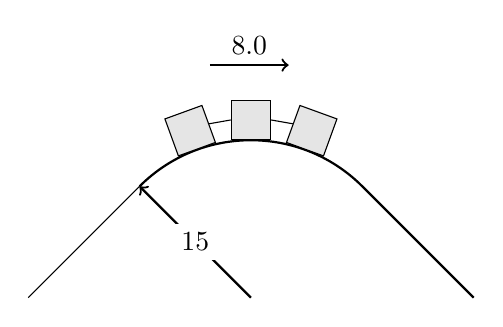
\begin{tikzpicture}
        \draw[thick] (135:2) arc (135:45:2) -- ++ (315:2);
        \node[fill=white!90!black,rectangle,anchor=south,rotate=+20,draw,minimum size=0.5cm] (A) at (110:2) {};
        \node[fill=white!90!black,rectangle,anchor=south,rotate=0,draw,minimum size=0.5cm] (B) at (90:2) {};
        \node[fill=white!90!black,rectangle,anchor=south,rotate=-20,draw,minimum size=0.5cm] (C) at (70:2) {};
        \draw (A.east) -- (B.west) (B.east) -- (C.west);
        \draw (135:2) -- ++ (225:2);
        \draw[thick,->] (0,0) -- (135:2) node[pos=0.5,anchor=center,fill=white] {\SI{15}{\meter}};
        \draw[thick,->] (100:3) -- ++(0:1) node[anchor=south,pos=0.5] {\SI{8.0}{\meter\per\second}};
    \end{tikzpicture}
    \end{center}
    The car passes over a hill of radius \SI{15}{\meter}, as shown. 
    At the top of the hill, the car has a speed of \SI{8.0}{\meter\per\second}.
    What is the force of the track on the car at the top of the hill?
    \begin{multicols}{2}
    \begin{choices}
        \wrongchoice{\SI{7.0}{\kilo\newton} up}
        \wrongchoice{\SI{7.0}{\kilo\newton} down}
        \wrongchoice{\SI{2.8}{\kilo\newton} down}
      \correctchoice{\SI{2.8}{\kilo\newton} up}
        \wrongchoice{\SI{5.6}{\kilo\newton} down}
    \end{choices}
    \end{multicols}
\end{question}
}

\element{serway-mc}{
\begin{question}{serway-ch06-q13}
    A \SI{0.20}{\kilo\gram} object attached to the end of a string swings in a vertical circle (radius = \SI{80}{\centi\meter}). 
    At the top of the circle the speed of the object is \SI{4.5}{\meter\per\second}. 
    What is the magnitude of the tension in the string at this position?
    \begin{multicols}{3}
    \begin{choices}
        \wrongchoice{\SI{7.0}{\newton}}
        \wrongchoice{\SI{2.0}{\newton}}
      \correctchoice{\SI{3.1}{\newton}}
        \wrongchoice{\SI{5.1}{\newton}}
        \wrongchoice{\SI{6.6}{\newton}}
    \end{choices}
    \end{multicols}
\end{question}
}

\element{serway-mc}{
\begin{question}{serway-ch06-q14}
    A roller-coaster car has a mass of \SI{500}{\kilo\gram} when fully loaded with passengers. 
    \begin{center}
    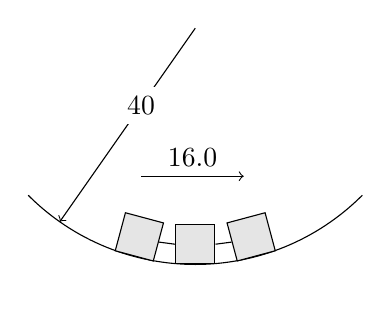
\begin{tikzpicture}
        \draw (225:3) arc (225:315:3);
        \draw[->] (0,0) -- (235:3) node[pos=0.4,fill=white,anchor=center] {\SI{40}{\meter}};
        \node[fill=white!90!black,rectangle,anchor=south,rotate=-15,draw,minimum size=0.5cm] (A) at (255:3) {};
        \node[fill=white!90!black,rectangle,anchor=south,rotate=0,draw,minimum size=0.5cm] (B) at (270:3) {};
        \node[fill=white!90!black,rectangle,anchor=south,rotate=+15,draw,minimum size=0.5cm] (C) at (285:3) {};
        \draw (A.east) -- (B.west) (B.east) -- (C.west);
        \draw[->] (250:2) -- ++(0:1.3) node[anchor=south,pos=0.5] {\SI{16.0}{\meter\per\second}};
    \end{tikzpicture}
    \end{center}
    At the bottom of a circular dip of radius \SI{40}{\meter} (as shown in the figure) the car has a speed of \SI{16}{\meter\per\second}. 
    What is the magnitude of the force of the track on the car at the bottom of the dip?
    \begin{multicols}{3}
    \begin{choices}
        \wrongchoice{\SI{3.2}{\kilo\newton}}
      \correctchoice{\SI{8.1}{\kilo\newton}}
        \wrongchoice{\SI{4.9}{\kilo\newton}}
        \wrongchoice{\SI{1.7}{\kilo\newton}}
        \wrongchoice{\SI{5.3}{\kilo\newton}}
    \end{choices}
    \end{multicols}
\end{question}
}

\element{serway-mc}{
\begin{question}{serway-ch06-q15}
    A \SI{0.50}{\kilo\gram} mass attached to the end of a string swings in a vertical circle (radius = \SI{2.0}{\meter}). 
    When the mass is at the highest point of the circle the speed of the mass is \SI{8.0}{\meter\per\second}. 
    What is the magnitude of the force of the string on the mass at this position?
    \begin{multicols}{3}
    \begin{choices}
        \wrongchoice{\SI{21}{\newton}}
      \correctchoice{\SI{11}{\newton}}
        \wrongchoice{\SI{16}{\newton}}
        \wrongchoice{\SI{26}{\newton}}
        \wrongchoice{\SI{36}{\newton}}
    \end{choices}
    \end{multicols}
\end{question}
}

\element{serway-mc}{
\begin{question}{serway-ch06-q16}
    A \SI{50}{\kilo\gram} child riding a Ferris wheel (radius = \SI{10}{\meter}) travels in a vertical circle. 
    The wheel completes one revolution every \SI{10}{\second}.
    What is the magnitude of the force on the child by the seat
        at the highest point on the circular path?
    \begin{multicols}{3}
    \begin{choices}
      \correctchoice{\SI{0.29}{\kilo\newton}}
        \wrongchoice{\SI{0.49}{\kilo\newton}}
        \wrongchoice{\SI{0.69}{\kilo\newton}}
        \wrongchoice{\SI{0.20}{\kilo\newton}}
        \wrongchoice{\SI{0.40}{\kilo\newton}}
    \end{choices}
    \end{multicols}
\end{question}
}

\element{serway-mc}{
\begin{question}{serway-ch06-q17}
    A \SI{0.30}{\kilo\gram} mass attached to the end of a string swings in a vertical circle (R = \SI{1.6}{\meter}), as shown. 
    \begin{center}
    \begin{tikzpicture}
        \draw[dashed] (0,0) circle (2cm);
        \draw[thick,->] (180:2.2) -- ++(270:0.75cm)
            node[pos=0.5,anchor=east] {$g$};
        \draw[dashed] (0,0) -- (270:2cm);
        \draw[fill] (320:2) circle (2pt)
            node[anchor=north west] {$m$};
        \draw[thick,->] (320:2) -- ++(50:1.5cm)
            node[pos=0.5,anchor=north west] {$v$};
        \draw[thick] (0,0) -- (320:2)
            node[pos=0.5,fill=white,anchor=center] {$R$};
        \draw[<->] (270:1.5) arc (270:320:1.5)
            node[font=\small,pos=0.5,anchor=center,fill=white] {$\theta$};
    \end{tikzpicture}
    \end{center}
    At an instant when $\theta=\ang{50}$,
        the tension in the string is \SI{8.0}{\newton}. 
    What is the magnitude of the resultant force on the mass at this instant?
    \begin{multicols}{3}
    \begin{choices}
        \wrongchoice{\SI{5.6}{\newton}}
        \wrongchoice{\SI{6.0}{\newton}}
      \correctchoice{\SI{6.5}{\newton}}
        \wrongchoice{\SI{5.1}{\newton}}
        \wrongchoice{\SI{2.2}{\newton}}
    \end{choices}
    \end{multicols}
\end{question}
}

\element{serway-mc}{
\begin{question}{serway-ch06-q18}
    An object attached to the end of a string swings in a vertical circle
        $\left(R=\SI{1.2}{\meter}\right)$, as shown. 
    \begin{center}
    \begin{tikzpicture}
        \draw[dashed] (0,0) circle (2cm);
        \draw[thick,->] (180:2.2) -- ++(270:0.75cm)
            node[pos=0.5,anchor=east] {$g$};
        \draw[dashed] (0,0) -- (0:2cm);
        \draw[fill] (30:2) circle (2pt)
            node[anchor=south west] {$m$};
        \draw[thick,->] (30:2) -- ++(300:1.5cm)
            node[pos=0.5,anchor=south west] {$v$};
        \draw[thick] (0,0) -- (30:2)
            node[pos=0.5,fill=white,anchor=center] {$R$};
        \draw[<->] (0:1.5) arc (0:30:1.5)
            node[font=\small,pos=0.5,anchor=center,fill=white] {$\theta$};
    \end{tikzpicture}
    \end{center}
    At an instant when $\theta=\ang{30}$,
        the speed of the object is \SI{5.1}{\meter\per\second} and the tension in the string has a magnitude of \SI{20}{\newton}.
    What is the mass of the object?
    \begin{multicols}{3}
    \begin{choices}
        \wrongchoice{\SI{2.0}{\kilo\gram}}
        \wrongchoice{\SI{1.5}{\kilo\gram}}
        \wrongchoice{\SI{1.8}{\kilo\gram}}
      \correctchoice{\SI{1.2}{\kilo\gram}}
        \wrongchoice{\SI{0.80}{\kilo\gram}}
    \end{choices}
    \end{multicols}
\end{question}
}

\element{serway-mc}{
\begin{question}{serway-ch06-q19}
    A \SI{0.40}{\kilo\gram} mass attached to the end of a string swings in a vertical circle having a radius of \SI{1.8}{\meter}. 
    At an instant when the string makes an angle of \num{40} degrees below the horizontal,
        the speed of the mass is \SI{5.0}{\meter\per\second}. 
    What is the magnitude of the tension in the string at this instant?
    \begin{multicols}{3}
    \begin{choices}
        \wrongchoice{\SI{9.5}{\newton}}
        \wrongchoice{\SI{3.0}{\newton}}
      \correctchoice{\SI{8.1}{\newton}}
        \wrongchoice{\SI{5.6}{\newton}}
        \wrongchoice{\SI{4.7}{\newton}}
    \end{choices}
    \end{multicols}
\end{question}
}

\element{serway-mc}{
\begin{question}{serway-ch06-q20}
    A \SI{0.50}{\kilo\gram} mass attached to the end of a string swings in a vertical circle (radius = \SI{2.0}{\meter}).
    When the string is horizontal, the speed of the mass is \SI{8.0}{\meter\per\second}.
    What is the magnitude of the force of the string on the mass at this position?
    \begin{multicols}{3}
    \begin{choices}
      \correctchoice{\SI{16}{\newton}}
        \wrongchoice{\SI{17}{\newton}}
        \wrongchoice{\SI{21}{\newton}}
        \wrongchoice{\SI{11}{\newton}}
        \wrongchoice{\SI{25}{\newton}}
    \end{choices}
    \end{multicols}
\end{question}
}

\element{serway-mc}{
\begin{question}{serway-ch06-q21}
    A \SI{4.0}{\kilo\gram} mass attached to the end of a string swings in a vertical circle of radius \SI{2.0}{\meter}. 
    \begin{center}
    \begin{tikzpicture}
        \draw[dashed] (0,0) circle (2cm);
        \draw[thick,->] (180:2.2) -- ++(270:0.75cm)
            node[pos=0.5,anchor=east] {$g$};
        \draw[dashed] (0,0) -- (270:2cm);
        \draw[fill] (305:2) circle (2pt)
            node[anchor=north west] {$m$};
        \draw[thick,->] (305:2) -- ++(35:1.5cm)
            node[pos=0.5,anchor=north west] {$v$};
        \draw[thick] (0,0) -- (305:2)
            node[pos=0.5,fill=white,anchor=center] {$R$};
        \draw[<->] (270:1.5) arc (270:305:1.5)
            node[font=\small,pos=0.5,anchor=north] {\ang{35}};
    \end{tikzpicture}
    \end{center}
    When the string makes an angle of \ang{35} with the vertical as shown,
        the speed of the mass is \SI{5.0}{\meter\per\second}.
    At this instant what is the magnitude of the force the string exerts on the mass?
    \begin{multicols}{3}
    \begin{choices}
        \wrongchoice{\SI{50}{\newton}}
      \correctchoice{\SI{82}{\newton}}
        \wrongchoice{\SI{89}{\newton}}
        \wrongchoice{\SI{11}{\newton}}
        \wrongchoice{\SI{61}{\newton}}
    \end{choices}
    \end{multicols}
\end{question}
}

\element{serway-mc}{
\begin{question}{serway-ch06-q22}
    A split highway has a number of lanes for traffic. 
    For traffic going in one direction,
        the radius for the inside of the curve is half the radius for the outside.
    One car, car $A$, travels on the inside while another car of equal mass, car $B$,
        travels at equal speed on the outside of the curve. 
    Which statement about resultant forces on the cars is correct?
    \begin{choices}
        \wrongchoice{The force on $A$ is half the force on $B$.}
      \correctchoice{The force on $B$ is half the force on $A$.}
        \wrongchoice{The force on $A$ is four times the force on $B$.}
        \wrongchoice{The force on $B$ is four times the force on $A$.}
        \wrongchoice{There is no net resultant force on either as long as they stay on the road while turning.}
    \end{choices}
\end{question}
}

\element{serway-mc}{
\begin{question}{serway-ch06-q23}
    A race car traveling at \SI{100}{\meter\per\second} enters an unbanked turn of \SI{400}{\meter} radius. 
    The coefficient of (static) friction between the tires and the track is \num{1.1}. 
    The track has both an inner and an outer wall. 
    Which statement is correct?
    \begin{choices}
      \correctchoice{The race car will crash into the outer wall.}
        \wrongchoice{The race car will crash into the inner wall.}
        \wrongchoice{The car will stay in the center of the track.}
        \wrongchoice{The car will stay in the center of the track if the driver speeds up.}
        \wrongchoice{The car would stay in the center of the track if the radius were reduced to \SI{200}{\meter}.}
    \end{choices}
\end{question}
}

\element{serway-mc}{
\begin{question}{serway-ch06-q24}
    A student is sitting on the right side of a school bus when it makes a right turn.
    We know that the force of gravity acts downwards and a normal force from the seat acts upwards. 
    %% NOTE: added ``with respect to the bus''
    If the student stays in place with respect to the bus when the bus turns,
        we also know that there must be
    \begin{choices}
        \wrongchoice{no other force on the student.}
        \wrongchoice{a force parallel to the seat directed forward on the student.}
        \wrongchoice{a force parallel to the seat directed to the left on the student.}
      \correctchoice{a force parallel to the seat directed to the right on the student.}
        \wrongchoice{a force parallel to the seat in a direction between forward and left on the student.}
    \end{choices}
\end{question}
}

\element{serway-mc}{
\begin{question}{serway-ch06-q25}
    For a plane to be able to fly clockwise in a horizontal circle as seen from above,
        in addition to exerting a force downwards on the air:
    \begin{choices}
        \wrongchoice{it must be increasing its speed.}
      \correctchoice{it must exert a force on the air that is directed to the plane's left side.}
        \wrongchoice{it must exert a force on the air that is directed to the plane's right side.}
        \wrongchoice{it does not need to exert a force: it must only move the wing flaps out.}
        \wrongchoice{it only needs to deflect the air without exerting any additional force on the air.}
    \end{choices}
\end{question}
}

\element{serway-mc}{
\begin{question}{serway-ch06-q26}
    When a car goes around a circular curve on a level road,
    \begin{choices}
        \wrongchoice{no frictional force is needed because the car simply follows the road.}
        \wrongchoice{the frictional force of the road on the car increases when the car's speed decreases.}
      \correctchoice{the frictional force of the road on the car increases when the car's speed increases.}
        \wrongchoice{the frictional force of the road on the car increases when the car moves to the outside of the curve.}
        \wrongchoice{there is no net frictional force because the road and the car exert equal and opposite forces on each other.}
    \end{choices}
\end{question}
}

\element{serway-mc}{
\begin{question}{serway-ch06-q27}
    An iceboat is traveling in a circle on the ice. 
    Halfway around the circle the sail and the steering mechanism fall off the boat. 
    Which statement is correct?
    \begin{choices}
        \wrongchoice{The boat will continue traveling in the circle because there is no friction.}
        \wrongchoice{The boat will continue to travel in the circle because its velocity exerts a force on it.}
      \correctchoice{The boat will move off on a line tangent to the circle because there is no force on it.}
        \wrongchoice{The boat will move off tangent to the circle because there is a force on it perpendicular to the boat directed to the outside of the circle.}
        \wrongchoice{The boat will move off to the outside perpendicular to the tangent line since a force directed to the outside of the circle always acts on the boat.}
    \end{choices}
\end{question}
}

%% T: tension
%% F: force
%% N: normal force
\element{serway-mc}{
\begin{question}{serway-ch06-q28}
    A rock attached to a string swings in a vertical circle. 
    Which free body diagram could correctly describe the force(s)
        on the rock when it is at the highest point?
    \begin{multicols}{2}
    \begin{choices}
        \AMCboxDimensions{down=-1.0cm}
        \wrongchoice{
            \begin{tikzpicture}
                \draw[white] (-1,-1) rectangle (+1,+1);
                \draw[fill] (0,0) circle (1.5pt);
                \draw[very thick,->] (0,0) -- ++ (270:0.75) node[anchor=north] {$W$};
            \end{tikzpicture}
        }
        \wrongchoice{
            \begin{tikzpicture}
                \draw[white] (-1,-1) rectangle (+1,+1);
                \draw[fill] (0,0) circle (1.5pt);
                \draw[very thick,->] (0,0) -- ++ (90:0.50) node[anchor=west] {$N$};
                \draw[very thick,->] (0,0) -- ++ (270:0.75) node[anchor=north] {$W$};
            \end{tikzpicture}
        }
        %% ANS is C
        \correctchoice{
            \begin{tikzpicture}
                \draw[white] (-1,-1) rectangle (+1,+1);
                \draw[fill] (0,0) circle (1.5pt);
                \draw[very thick,->] (0.2,0) -- ++ (270:0.50) node[anchor=west] {$T$};
                \draw[very thick,->] (0,0) -- ++ (270:0.75) node[anchor=north] {$W$};
            \end{tikzpicture}
        }
        \wrongchoice{
            \begin{tikzpicture}
                \draw[white] (-1,-1) rectangle (+1,+1);
                \draw[fill] (0,0) circle (1.5pt);
                \draw[very thick,->] (0,0) -- ++ (270:0.75) node[anchor=north] {$T$};
            \end{tikzpicture}
        }
        \wrongchoice{
            \begin{tikzpicture}
                \draw[white] (-1,-1) rectangle (+1,+1);
                \draw[fill] (0,0) circle (1.5pt);
                \draw[very thick,->] (0,0) -- ++ (0:0.5) node[anchor=south] {$F$};
                \draw[very thick,->] (0.2,0) -- ++ (270:0.50) node[anchor=west] {$T$};
                \draw[very thick,->] (0,0) -- ++ (270:0.75) node[anchor=north] {$W$};
            \end{tikzpicture}
        }
    \end{choices}
    \end{multicols}
\end{question}
}


%% NOTE: alternative question from Six Easy Lesson, p33
%% NOTE: include diagram of spinning object on string?
% A ball swings at the end of a string in a circular path in a vertical plane.
% Which free-body diagram best represents the forces acting on the ball when at the bottom of the circle and moving toward the right?
% The ball moves at constants speed.

\element{serway-mc}{
\begin{question}{serway-ch06-q29}
    A rock attached to a string swings in a vertical circle. 
    Which free body diagram could correctly describe the force(s) 
        on the rock when the string is in one possible horizontal position?
    \begin{multicols}{2}
    \begin{choices}
        \AMCboxDimensions{down=-0.8cm}
        \wrongchoice{
            \begin{tikzpicture}
                \draw[white] (-1,-1) rectangle (+1,+1);
                \draw[fill] (0,0) circle (1.5pt);
                \draw[very thick,->] (0,0) -- ++ (180:0.75) node[anchor=north] {$T$};
            \end{tikzpicture}
        }
        \wrongchoice{
            \begin{tikzpicture}
                \draw[white] (-1,-1) rectangle (+1,+1);
                \draw[fill] (0,0) circle (1.5pt);
                \draw[very thick,->] (0,0) -- ++ (270:0.75) node[anchor=north] {$W$};
            \end{tikzpicture}
        }
        %% ANS is C
        \correctchoice{
            \begin{tikzpicture}
                \draw[white] (-1,-1) rectangle (+1,+1);
                \draw[fill] (0,0) circle (1.5pt);
                \draw[very thick,->] (0,0) -- ++ (180:0.75) node[anchor=north west] {$T$};
                \draw[very thick,->] (0,0) -- ++ (270:0.75) node[anchor=north] {$W$};
            \end{tikzpicture}
        }
        \wrongchoice{
            \begin{tikzpicture}
                \draw[white] (-1,-1) rectangle (+1,+1);
                \draw[fill] (0,0) circle (1.5pt);
                \draw[very thick,->] (0,0) -- ++ (180:0.75) node[anchor=north west] {$T$};
                \draw[very thick,->] (0,0) -- ++ (0:0.75) node[anchor=north] {$N$};
                \draw[very thick,->] (0,0) -- ++ (270:0.75) node[anchor=north] {$W$};
            \end{tikzpicture}
        }
        \wrongchoice{
            \begin{tikzpicture}
                \draw[white] (-1,-1) rectangle (+1,+1);
                \draw[fill] (0,0) circle (1.5pt);
                \draw[very thick,->] (0,0) -- ++ (180:0.75) node[anchor=north] {$T$};
                \draw[very thick,->] (0,0) -- ++ (90:0.75) node[anchor=north west] {$N$};
                \draw[very thick,->] (0,0) -- ++ (270:0.75) node[anchor=north] {$W$};
            \end{tikzpicture}
        }
    \end{choices}
    \end{multicols}
\end{question}
}

\element{serway-mc}{
\begin{question}{serway-ch06-q30}
    A rock attached to a string swings in a vertical circle. 
    Which free body diagram could correctly describe the force(s)
        on the rock when it is at the lowest point?
    \begin{multicols}{2}
    \begin{choices}
        \AMCboxDimensions{down=-1.0cm}
        \wrongchoice{
            \begin{tikzpicture}
                \draw[white] (-1,-1.5) rectangle (+1,+1.5);
                \draw[fill] (0,0) circle (1.5pt);
                \draw[very thick,->] (0,0) -- ++ (270:1) node[anchor=north] {$W$};
            \end{tikzpicture}
        }
        \correctchoice{
            \begin{tikzpicture}
                \draw[white] (-1,-1.5) rectangle (+1,+1.5);
                \draw[fill] (0,0) circle (1.5pt);
                \draw[very thick,->] (0,0) -- ++ (270:1) node[anchor=north] {$W$};
                \draw[very thick,->] (0,0) -- ++ (90:1.5) node[anchor=north west] {$T$};
            \end{tikzpicture}
        }
        \wrongchoice{
            \begin{tikzpicture}
                \draw[white] (-1,-1.5) rectangle (+1,+1.5);
                \draw[fill] (0,0) circle (1.5pt);
                \draw[very thick,->] (0,0) -- ++ (90:1.5) node[anchor=north west] {$T$};
            \end{tikzpicture}
        }
        \wrongchoice{
            \begin{tikzpicture}
                \draw[white] (-1,-1.5) rectangle (+1,+1.5);
                \draw[fill] (0,0) circle (1.5pt);
                \draw[very thick,->] (0,0) -- ++ (270:1) node[anchor=north] {$N$};
                \draw[very thick,->] (0,0) -- ++ (90:1) node[anchor=north west] {$T$};
            \end{tikzpicture}
        }
        \wrongchoice{
            \begin{tikzpicture}
                \draw[white] (-1,-1.5) rectangle (+1,+1.5);
                \draw[fill] (0,0) circle (1.5pt);
                \draw[very thick,->] (0,0) -- ++ (0:0.5) node[anchor=north] {$F$};
                \draw[very thick,->] (0,0) -- ++ (270:1) node[anchor=north] {$W$};
                \draw[very thick,->] (0,0) -- ++ (90:1) node[anchor=north west] {$T$};
            \end{tikzpicture}
        }
    \end{choices}
    \end{multicols}
\end{question}
}

\element{serway-mc}{
\begin{question}{serway-ch06-q31}
    Two small cylindrical plastic containers with flat bottoms are placed on a turntable that has a smooth flat surface. 
    Canister $A$ is empty; canister $B$ contains lead shot. 
    Each canister is the same distance $r$ from the center. 
    The coefficient of static friction between the canisters and the turntable is $\mu_s$. 
    When the speed of the turntable is gradually increased,
    \begin{choices}
        \wrongchoice{only the lighter container slides outward off the turntable; the heavier one stays on.}
        \wrongchoice{only the heavier container slides outward off the turntable; the lighter one stays on.}
      \correctchoice{both containers slide off the turntable at the same turntable speed.}
        \wrongchoice{the lighter container slides inward.}
        \wrongchoice{the heavier container slides inward.}
    \end{choices}
\end{question}
}

\element{serway-mc}{
\begin{question}{serway-ch06-q32}
    A hornet circles around a pop can at increasing speed while
        flying in a path with a \SI{12}{\centi\meter} diameter. 
    We can conclude that the hornet's wings must push on the air
        with force components that are
    \begin{choices}
        \wrongchoice{straight down.}
        \wrongchoice{down and inwards.}
      \correctchoice{down and outwards.}
        \wrongchoice{down and backwards.}
        \wrongchoice{down, inwards and backwards.}
    \end{choices}
\end{question}
}

\element{serway-mc}{
\begin{question}{serway-ch06-q33}
    A hornet circles around a pop can at constant speed once per second in a path with a \SI{12}{\centi\meter} diameter. 
    We can conclude that the hornet's wings must push on the air with force components that are:
    \begin{choices}
        \wrongchoice{straight down.}
        \wrongchoice{down and inwards.}
        \wrongchoice{down and outwards.}
        \wrongchoice{down and backwards.}
      \correctchoice{down, backwards and outwards.}
    \end{choices}
\end{question}
}

\element{serway-mc}{
\begin{question}{serway-ch06-q34}
    Frank says that if you release the string when swinging a ball in a horizontal circle,
        the ball flies out in the radial direction defined by the string at the instant you release the ball. 
    John says that it flies out along a tangent line perpendicular to the string,
        and that it then drops straight down to the ground. 
    Which one, if either, is correct?
    \begin{choices}
        \wrongchoice{Frank, because the centrifugal force is no longer counteracted by the string.}
        \wrongchoice{Frank, because balls naturally fly straight out.}
        \wrongchoice{John, because there is no centrifugal force.}
        \wrongchoice{John, because balls fall straight down when released.}
      \correctchoice{Neither, because although there is no centrifugal force, and the ball's velocity is tangent to the circle at the instant of release, the ball then follows a parabolic trajectory.}
    \end{choices}
\end{question}
}

\element{serway-mc}{
\begin{question}{serway-ch06-q35}
    The equation below is the solution to a problem.
    \begin{align*}
        & \dfrac{\left(\SI{2.00}{\kilo\gram}\right)\left(\SI{8.00}{\meter\per\second\squared}\right)^2}{\left(\SI{5.00}{\meter}\right)} = \\
        &\quad\quad \SI{6.00}{\newton} - \left(\SI{2.00}{\kilo\gram}\right)\left(\SI{9.8}{\meter\per\second\squared}\right)\left(\cos\ang{180}\right)
    \end{align*}
    The best physical representation of this equation is:
    \begin{choices}
        \wrongchoice{a sphere of \SI{2.00}{\kilo\gram} mass under a \SI{6.00}{\newton} tension when at the bottom of a vertical circle.}
        \wrongchoice{a sphere of \SI{2.00}{\kilo\gram} mass under a \SI{6.00}{\newton} tension when at the side of a vertical circle.}
      \correctchoice{a sphere of \SI{2.00}{\kilo\gram} mass under a \SI{6.00}{\newton} tension when at the top of a vertical circle.}
        \wrongchoice{a sphere of \SI{2.00}{\kilo\gram} mass at any point on a horizontal circle.}
        \wrongchoice{a \SI{2.00}{\kilo\gram} gecko running on the ceiling with a speed of \SI{8.00}{\meter\per\second}.}
    \end{choices}
\end{question}
}

\element{serway-mc}{
\begin{question}{serway-ch06-q36}
    The equation below is the solution to a problem.
    \begin{align*}
        & \dfrac{\left(\SI{2.00}{\kilo\gram}\right)\left(\SI{8.00}{\meter\per\second\squared}\right)^2}{\left(\SI{5.00}{\meter}\right)} = \\
        &\quad\quad = \SI{6.00}{\newton} - \left(\SI{2.00}{\kilo\gram}\right)\left(\SI{9.8}{\meter\per\second\squared}\right)\left(\cos\ang{0}\right)
    \end{align*}
    The best physical representation of this equation is:
    \begin{choices}
      \correctchoice{a sphere of \SI{2.00}{\kilo\gram} mass under a \SI{6.00}{\newton} tension when at the bottom of a vertical circle.}
        \wrongchoice{a sphere of \SI{2.00}{\kilo\gram} mass under a \SI{6.00}{\newton} tension when at the side of a vertical circle.}
        \wrongchoice{a sphere of \SI{2.00}{\kilo\gram} mass under a \SI{6.00}{\newton} tension when at the top of a vertical circle.}
        \wrongchoice{a sphere of \SI{2.00}{\kilo\gram} mass at any point on a horizontal circle.}
        \wrongchoice{a \SI{2.00}{\kilo\gram} gecko running on the ceiling with a speed of \SI{8.00}{\meter\per\second}.}
    \end{choices}
\end{question}
}

\element{serway-mc}{
\begin{question}{serway-ch06-q37}
    The equation below is the solution to a problem.
    \begin{align*}
        & \dfrac{\left(\SI{2.00}{\kilo\gram}\right)\left(\SI{8.00}{\meter\per\second\squared}\right)^2}{\left(\SI{5.00}{\meter}\right)} = \\
        &\quad\quad \SI{6.00}{\newton} - \left(\SI{2.00}{\kilo\gram}\right)\left(\SI{9.8}{\meter\per\second\squared}\right)\left(\cos\ang{90}\right)
    \end{align*}
    The best physical representation of this equation is:
    \begin{choices}
        \wrongchoice{a sphere of \SI{2.00}{\kilo\gram} mass under a \SI{6.00}{\newton} tension when at the bottom of a vertical circle.}
      \correctchoice{a sphere of \SI{2.00}{\kilo\gram} mass under a \SI{6.00}{\newton} tension when at the side of a vertical circle.}
        \wrongchoice{a sphere of \SI{2.00}{\kilo\gram} mass under a \SI{6.00}{\newton} tension when at the top of a vertical circle.}
        \wrongchoice{a sphere of \SI{2.00}{\kilo\gram} mass at any point on a horizontal circle.}
        \wrongchoice{a \SI{2.00}{\kilo\gram} gecko running on the ceiling with a speed of \SI{8.00}{\meter\per\second}.}
    \end{choices}
\end{question}
}

\element{serway-mc}{
\begin{question}{serway-ch06-q38}
    The coefficient of static friction for the tires of a race car is \num{0.950} and the coefficient of kinetic friction is \num{0.800}. 
    The car is on a level circular track of \SI{50.0}{\meter} radius on a planet where $g=\SI{2.45}{\meter\per\second\squared}$ compared to Earth's $g=\SI{9.80}{\meter\per\second\squared}$.
    The maximum safe speed on the track on the planet is \rule[-0.1pt]{4em}{0.1pt} times as large as the maximum safe speed on Earth.
    \begin{multicols}{3}
    \begin{choices}
        \wrongchoice{\num{0.25}}
      \correctchoice{\num{0.50}}
        \wrongchoice{\num{1.00}}
        \wrongchoice{\num{2.00}}
        \wrongchoice{\num{4.00}}
    \end{choices}
    \end{multicols}
\end{question}
}

\element{serway-mc}{
\begin{question}{serway-ch06-q39}
    The coefficient of static friction for the tires of a race car is \num{0.950} and the coefficient of kinetic friction is \num{0.800}. 
    The car is on a level circular track of \SI{50.0}{\meter} radius on a planet where $g=\SI{2.45}{\meter\per\second\squared}$ compared to Earth's $g=\SI{9.80}{\meter\per\second\squared}$.
    If the car is to be able to travel at the same speed on the planet as on Earth,
        the radius of the track on the planet must be \rule[-0.1pt]{4em}{0.1pt} times as large as the radius of the track on Earth.
    \begin{multicols}{3}
    \begin{choices}
        \wrongchoice{\num{0.25}}
        \wrongchoice{\num{0.50}}
        \wrongchoice{\num{1.00}}
        \wrongchoice{\num{2.00}}
      \correctchoice{\num{4.00}}
    \end{choices}
    \end{multicols}
\end{question}
}

\element{serway-mc}{
\begin{question}{serway-ch06-q40}
    A boy on board a cruise ship drops a \SI{30.0}{\gram} marble into the ocean. 
    If the resistive force proportionality constant is \SI{0.500}{\kilo\gram\per\second},
        what is the terminal speed of the marble?
    \begin{multicols}{2}
    \begin{choices}
        \wrongchoice{\SI{0.147}{\meter\per\second}}
        \wrongchoice{\SI{0.294}{\meter\per\second}}
      \correctchoice{\SI{0.588}{\meter\per\second}}
        \wrongchoice{\SI{1.18}{\meter\per\second}}
        \wrongchoice{\SI{2.35}{\meter\per\second}}
    \end{choices}
    \end{multicols}
\end{question}
}

\element{serway-mc}{
\begin{question}{serway-ch06-q41}
    In a recent mystery,
        the hero saves himself by spreading out a windshield tarpaulin to reduce his terminal velocity. 
    A skydiver of \SI{75}{\kilo\gram} mass has a terminal velocity of \SI{60}{\meter\per\second}.
    If the hero has the same \SI{75}{\kilo\gram} mass,
        the same density as the sky diver,
        and a drag coefficient twice as large with the tarp,
        by what factor is his effective area greater than the \SI{0.70}{\meter\squared} area of the skydiver?
    \begin{multicols}{3}
    \begin{choices}
        \wrongchoice{\num{4}}
        \wrongchoice{\num{8}}
        \wrongchoice{\num{16}}
      \correctchoice{\num{32}}
        \wrongchoice{\num{64}}
    \end{choices}
    \end{multicols}
\end{question}
}

\element{serway-mc}{
\begin{question}{serway-ch06-q42}
    The following equation was obtained by solving a physics problem:
    \begin{equation*}
        \dfrac{\left(\SI{16.0}{\meter\per\second}\right)^2}
              {\left(\SI{75.0}{\meter}\right)\left(\SI{9.80}{\meter\per\second\squared}\right)}
          = \tan\ang{19.2}
    \end{equation*}
    The best physical representation of the situation is:
    \begin{choices}
        \wrongchoice{A car traveling at \SI{16.0}{\meter\per\second} is \ang{19.2} into a turn of a quarter circle on a level road.}
        \wrongchoice{A mass on a string that is originally horizontal has fallen to where the angle between the string and the vertical direction is \ang{19.2}.}
        \wrongchoice{A mass on a string originally horizontal has fallen \ang{19.2} from the horizontal direction.}
      \correctchoice{A car traveling at \SI{16.0}{\meter\per\second} is on a circular curve banked at \ang{19.2}.}
        \wrongchoice{A car traveling at \SI{16.0}{\meter\per\second} and going over a semicircular mountain-top road is \ang{19.2} down from the top.}
    \end{choices}
\end{question}
}

\element{serway-mc}{
\begin{question}{serway-ch06-q43}
    An airplane flies in a horizontal circle of radius \SI{500}{\meter}
        at a speed of \SI{150}{\meter\per\second}.
    If the plane were to fly in the same \SI{500}{\meter} circle
        at a speed of \SI{300}{\meter\per\second},
        by what factor would its centripetal acceleration change?
    \begin{multicols}{3}
    \begin{choices}
        \wrongchoice{\num{0.25}}
        \wrongchoice{\num{0.50}}
        \wrongchoice{\num{1.00}}
        \wrongchoice{\num{2.00}}
      \correctchoice{\num{4.00}}
    \end{choices}
    \end{multicols}
\end{question}
}

\element{serway-mc}{
\begin{question}{serway-ch06-q44}
    An airplane flies in a horizontal circle of radius \SI{500}{\meter}
        at a speed of \SI{150}{\meter\per\second}.
    If the radius were changed to \SI{1000}{\meter},
        but the speed remained the same,
        by what factor would its centripetal acceleration change?
    \begin{multicols}{3}
    \begin{choices}
        \wrongchoice{\num{0.25}}
      \correctchoice{\num{0.50}}
        \wrongchoice{\num{1.00}}
        \wrongchoice{\num{2.00}}
        \wrongchoice{\num{4.00}}
    \end{choices}
    \end{multicols}
\end{question}
}

\element{serway-mc}{
\begin{question}{serway-ch06-q45}
    An airplane flies in a horizontal circle of radius \SI{500}{\meter}
        at a speed of \SI{150}{\meter\per\second}.
    %% changed wording, removed ``same''
    If the radius were changed to \SI{1000}{\meter},
        and the speed to \SI{300}{\meter\per\second},
        by what factor would its centripetal acceleration change?
    \begin{multicols}{3}
    \begin{choices}
        \wrongchoice{\num{0.25}}
        \wrongchoice{\num{0.50}}
        \wrongchoice{\num{1.00}}
      \correctchoice{\num{2.00}}
        \wrongchoice{\num{4.00}}
    \end{choices}
    \end{multicols}
\end{question}
}

\element{serway-mc}{
\begin{question}{serway-ch06-q46}
    A car enters a level,
        unbanked semi-circular hairpin turn of \SI{100}{\meter}
        radius at a speed of \SI{28}{\meter\per\second}. 
    The coefficient of friction between the tires and the road is $\mu=\num{0.800}$.
    If the car maintains a constant speed of \SI{28}{\meter\per\second},
        it will:
    \begin{choices}
        \wrongchoice{attempt to dig into the road surface.}
        \wrongchoice{tend to veer toward the center of the semicircle.}
      \correctchoice{arrive safely at the end of the semicircle.}
        \wrongchoice{tend to veer toward the outside of the circle.}
        \wrongchoice{veer toward the center for the first quarter-circle, then veer toward the outside for the second quarter-circle.}
    \end{choices}
\end{question}
}

\element{serway-mc}{
\begin{question}{serway-ch06-q47}
    A car enters a level,
        unbanked semi-circular hairpin turn of \SI{100}{\meter}
        radius at a speed of \SI{40}{\meter\per\second}. 
    The coefficient of friction between the tires and the road is $\mu=\num{0.25}$.
    If the car maintains a constant speed of \SI{40}{\meter\per\second},
        it will:
    \begin{choices}
        \wrongchoice{attempt to dig into the road surface.}
        \wrongchoice{tend to veer toward the center of the semicircle.}
        \wrongchoice{arrive safely at the end of the semicircle.}
      \correctchoice{tend to veer toward the outside of the circle.}
        \wrongchoice{veer toward the center for the first quarter-circle, then veer toward the outside for the second quarter-circle.}
    \end{choices}
\end{question}
}

\endinput




%% Halliday

%%--------------------------------------------------
%% Halliday: Fundamentals of Physics
%%--------------------------------------------------


%% Chapter 05: Force and Motion--I
%%--------------------------------------------------


%% Learning Objectives
%%--------------------------------------------------

%% 5.01: Identify that a force is a vector quantity and thus has both magnitude and direction and also components.
%% 5.02: Given two or more forces acting on the same particle, add the forces as vectors to get the net force.
%% 5.03: Identify Newton's first and second laws of motion.
%% 5.04: Identify inertial reference frames.
%% 5.05: Sketch a free-body diagram for an object, showing the object as a particle and drawing the forces acting on it as vectors with their tails anchored on the particle.
%% 5.06: Apply the relationship (Newton's second law) between the net force on an object, the mass of the object, and the acceleration produced by the net force.
%% 5.07: Identify that only external forces on an object can cause the object to accelerate


%% Halliday Multiple Choice Questions
%%--------------------------------------------------
\element{halliday-mc}{
\begin{question}{halliday-ch05-q01}
    An example of an inertial reference frame is:
    \begin{choices}
        \wrongchoice{any reference frame that is not accelerating}
      \correctchoice{a frame attached to a particle on which there are no forces}
        \wrongchoice{any reference frame that is at rest}
        \wrongchoice{a reference frame attached to the center of the universe}
        \wrongchoice{a reference frame attached to Earth}
    \end{choices}
\end{question}
}

\element{halliday-mc}{
\begin{question}{halliday-ch05-q02}
    An object moving at constant velocity in an inertial frame must:
    \begin{choices}
        \wrongchoice{have a net force on it}
        \wrongchoice{eventually stop due to gravity}
        \wrongchoice{not have any force of gravity on it}
      \correctchoice{have zero net force on it}
        \wrongchoice{have no frictional force on it}
    \end{choices}
\end{question}
}

\element{halliday-mc}{
\begin{question}{halliday-ch05-q03}
    In SI units a force is numerically equal to the \rule[-0.1pt]{4em}{0.1pt}  when the force is applied to it.
    \begin{choices}
        \wrongchoice{velocity of the standard kilogram}
        \wrongchoice{speed of the standard kilogram}
        \wrongchoice{velocity of any object}
      \correctchoice{acceleration of the standard kilogram}
        \wrongchoice{acceleration of any object}
    \end{choices}
\end{question}
}

\element{halliday-mc}{
\begin{question}{halliday-ch05-q04}
    Which of the following quantities is \emph{not} a vector?
    \begin{multicols}{2}
    \begin{choices}
      \correctchoice{Mass}
        \wrongchoice{Displacement}
        \wrongchoice{Weight}
        \wrongchoice{Acceleration}
        \wrongchoice{Force}
    \end{choices}
    \end{multicols}
\end{question}
}

\element{halliday-mc}{
\begin{question}{halliday-ch05-q05}
    A newton is the force:
    \begin{choices}
        \wrongchoice{of gravity on a \SI{1}{\kilo\gram} body}
        \wrongchoice{of gravity on a \SI{1}{\gram} body}
        \wrongchoice{that gives a \SI{1}{\gram} body an acceleration of \SI{1}{\centi\meter\per\second\squared}}
      \correctchoice{that gives a \SI{1}{\kilo\gram} body an acceleration of \SI{1}{\meter\per\second\squared}}
        \wrongchoice{that gives a \SI{1}{\kilo\gram} body an acceleration of \SI{9.8}{\meter\per\second\squared}}
    \end{choices}
\end{question}
}

\element{halliday-mc}{
\begin{question}{halliday-ch05-q06}
    The unit of force called the newton is:
    \begin{multicols}{2}
    \begin{choices}
        \wrongchoice{\SI{9.8}{\kilo\gram\meter\per\second}}
      \correctchoice{\SI{1}{\kilo\gram\meter\per\second\squared}}
        \wrongchoice{defined by means of Newton's third law}
        \wrongchoice{\SI{1}{\kilo\gram} of mass}
        \wrongchoice{\SI{1}{\kilo\gram} of force}
    \end{choices}
    \end{multicols}
\end{question}
}

\element{halliday-mc}{
\begin{question}{halliday-ch05-q07}
    A force of \SI{1}{\newton} is:
    \begin{multicols}{3}
    \begin{choices}
        \wrongchoice{\SI{1}{\kilo\gram\per\second}}
        \wrongchoice{\SI{1}{\kilo\gram\meter\per\second}}
      \correctchoice{\SI{1}{\kilo\gram\meter\per\second\squared}}
        \wrongchoice{\SI{1}{\kilo\gram\meter\squared\per\second}}
        \wrongchoice{\SI{1}{\kilo\gram\meter\squared\per\second\squared}}
    \end{choices}
    \end{multicols}
\end{question}
}

\element{halliday-mc}{
\begin{question}{halliday-ch05-q08}
    The standard \SI{1}{\kilo\gram} mass is attached to a compressed spring and the spring is released.
    If the mass initially has an acceleration of \SI{5.6}{\meter\per\second\squared},
        the force of the spring has a magnitude of:
    \begin{multicols}{2}
    \begin{choices}
        \wrongchoice{\SI{2.8}{\newton}}
      \correctchoice{\SI{5.6}{\newton}}
        \wrongchoice{\SI{11.2}{\newton}}
        \wrongchoice{zero}
        \wrongchoice{an undetermined amount}
    \end{choices}
    \end{multicols}
\end{question}
}

\element{halliday-mc}{
\begin{question}{halliday-ch05-q09}
    Acceleration is always in the direction:
    \begin{choices}
        \wrongchoice{of the displacement}
        \wrongchoice{of the initial velocity}
        \wrongchoice{of the final velocity}
      \correctchoice{of the net force}
        \wrongchoice{opposite to the frictional force}
    \end{choices}
\end{question}
}

\element{halliday-mc}{
\begin{question}{halliday-ch05-q10}
    The term ``mass'' refers to the same physical concept as:
    \begin{multicols}{2}
    \begin{choices}
        \wrongchoice{weight}
      \correctchoice{inertia}
        \wrongchoice{force}
        \wrongchoice{acceleration}
        \wrongchoice{volume}
    \end{choices}
    \end{multicols}
\end{question}
}

\element{halliday-mc}{
\begin{question}{halliday-ch05-q11}
    The inertia of a body tends to cause the body to:
    \begin{choices}
        \wrongchoice{speed up}
        \wrongchoice{slow down}
      \correctchoice{resist any change in its motion}
        \wrongchoice{fall toward Earth}
        \wrongchoice{decelerate due to friction}
    \end{choices}
\end{question}
}

\element{halliday-mc}{
\begin{question}{halliday-ch05-q12}
    A heavy ball is suspended as shown.
    \begin{center}
    \begin{tikzpicture}
        \node[anchor=south,fill,pattern=north east lines,minimum width=4cm, minimum height=0.05cm] at (0,0) {};
        \draw (-2,0) -- (2,0);
        \node[draw,fill=white!90!black,circle,minimum size=1cm] (M) at (0,-2) {};
        \draw (0,0) -- (M.north) node[pos=0.5,anchor=west] {upper string};
        \draw (M.south) -- ++(270:1.5) node[pos=0.5,anchor=west] {lower string};
    \end{tikzpicture}
    \end{center}
    A quick jerk on the lower string will break that string but a slow pull on the lower string will break the upper string.
    The first result occurs because:
    \begin{choices}
        \wrongchoice{the force is too small to move the ball}
        \wrongchoice{action and reaction is operating}
      \correctchoice{the ball has inertia}
        \wrongchoice{air friction holds the ball back}
        \wrongchoice{the ball has too much energy}
    \end{choices}
\end{question}
}

\element{halliday-mc}{
\begin{question}{halliday-ch05-q13}
    When a certain force is applied to the standard kilogram its acceleration is \SI{5.0}{\meter\per\second\squared}.
    When the same force is applied to another object its acceleration is one-fifth as much.
    The mass of the object is:
    \begin{multicols}{3}
    \begin{choices}
        \wrongchoice{\SI{0.2}{\kilo\gram}}
        \wrongchoice{\SI{0.5}{\kilo\gram}}
        \wrongchoice{\SI{1.0}{\kilo\gram}}
      \correctchoice{\SI{5.0}{\kilo\gram}}
        \wrongchoice{\SI{10}{\kilo\gram}}
    \end{choices}
    \end{multicols}
\end{question}
}

\element{halliday-mc}{
\begin{question}{halliday-ch05-q14}
    Mass differs from weight in that:
    \begin{choices}
        \wrongchoice{all objects have weight but some lack mass}
      \correctchoice{weight is a force and mass is not}
        \wrongchoice{the mass of an object is always more than its weight}
        \wrongchoice{mass can be expressed only in the metric system}
        \wrongchoice{there is no difference}
    \end{choices}
\end{question}
}

\element{halliday-mc}{
\begin{question}{halliday-ch05-q15}
    The mass of a body:
    \begin{choices}
        \wrongchoice{is slightly different at different places on Earth}
        \wrongchoice{is a vector}
      \correctchoice{is independent of the free-fall acceleration}
        \wrongchoice{is the same for all bodies of the same volume}
        \wrongchoice{can be measured most accurately on a spring scale}
    \end{choices}
\end{question}
}

\element{halliday-mc}{
\begin{question}{halliday-ch05-q16}
    The mass and weight of a body:
    \begin{choices}
        \wrongchoice{differ by a factor of 9.8}
        \wrongchoice{are identical}
        \wrongchoice{are the same physical quantities expressed in different units}
        \wrongchoice{are both a direct measure of the inertia of the body}
      \correctchoice{have the same ratio as that of any other body placed at that location}
    \end{choices}
\end{question}
}

\element{halliday-mc}{
\begin{question}{halliday-ch05-q17}
    An object placed on an equal-arm balance requires \SI{12}{\kilo\gram} to balance it.
    When placed on a spring scale, the scale reads \SI{12}{\kilo\gram}.
    Everything (balance, scale, set of weights and object) is now transported to the Moon where the free-fall acceleration is one-sixth that on Earth.
    The new readings of the balance and spring scale (respectively) are:
    \begin{multicols}{2}
    \begin{choices}
        \wrongchoice{\SI{12}{\kilo\gram}, \SI{12}{\kilo\gram}}
        \wrongchoice{\SI{2}{\kilo\gram}, \SI{2}{\kilo\gram}}
      \correctchoice{\SI{12}{\kilo\gram}, \SI{2}{\kilo\gram}}
        \wrongchoice{\SI{2}{\kilo\gram}, \SI{12}{\kilo\gram}}
        \wrongchoice{\SI{12}{\kilo\gram}, \SI{72}{\kilo\gram}}
    \end{choices}
    \end{multicols}
\end{question}
}

\element{halliday-mc}{
\begin{question}{halliday-ch05-q18}
    Two objects, one having three times the mass of the other,
        are dropped from the same height in a vacuum.
    At the end of their fall, their velocities are equal because:
    \begin{choices}
        \wrongchoice{anything falling in vacuum has constant velocity}
        \wrongchoice{all objects reach the same terminal velocity}
        \wrongchoice{the acceleration of the larger object is three times greater than that of the smaller object}
        \wrongchoice{the force of gravity is the same for both objects}
      \correctchoice{none of the provided}
    \end{choices}
\end{question}
}

\element{halliday-mc}{
\begin{question}{halliday-ch05-q19}
    A feather and a lead ball are dropped from rest in vacuum on the Moon.
    The acceleration of the feather is:
    \begin{choices}
        \wrongchoice{more than that of the lead ball}
      \correctchoice{the same as that of the lead ball}
        \wrongchoice{less than that of the lead ball}
        \wrongchoice{\SI{9.8}{\meter\per\second\squared}}
        \wrongchoice{zero since it floats in a vacuum}
    \end{choices}
\end{question}
}

\element{halliday-mc}{
\begin{question}{halliday-ch05-q20}
    The block shown moves with constant velocity on a horizontal surface.
    Two of the forces on it are shown.
    \begin{center}
    \begin{tikzpicture}
        %% Ground
        \node[anchor=north,fill,pattern=north east lines,minimum width=4cm,minimum height=0.05cm] at (0,0) {};
        \draw (-2,0) -- (2,0);
        %% Mass
        \node[draw,fill=white!90!black,minimum size=1.22cm,anchor=south] (M) at (0,0) {};
        %% Vectors
        \draw[thick,->] (M.east) -- ++(0:1.5cm) node[anchor=south,pos=0.5] {\SI{5}{\newton}};
        \draw[thick,->] (M.west) -- ++(180:0.9cm) node[anchor=south,pos=0.5] {\SI{3}{\newton}};
    \end{tikzpicture}
    \end{center}
    A frictional force exerted by the surface is the only other horizontal force on the block.
    The frictional force is:
    \begin{choices}
        \wrongchoice{zero}
      \correctchoice{\SI{2}{\newton}, leftward}
        \wrongchoice{\SI{2}{\newton}, rightward}
        \wrongchoice{slightly more than \SI{2}{\newton}, leftward}
        \wrongchoice{slightly less than \SI{2}{\newton}, leftward}
    \end{choices}
\end{question}
}

\element{halliday-mc}{
\begin{question}{halliday-ch05-q21}
    Two forces, one with a magnitude of \SI{3}{\newton} and the other with a magnitude of \SI{5}{\newton},
        are applied to an object.
    For which orientations of the forces shown in the diagrams is the magnitude of the acceleration of the object the least?
    \begin{multicols}{2}
    \begin{choices}
        %% ANS: is A
        \AMCboxDimensions{down=-0.8cm}
        \correctchoice{
            \begin{tikzpicture}
                \draw[white] (-1,-1) rectangle (1.5,1);
                \node[draw,fill=white!90!black,minimum size=0.25cm,anchor=center] (M) at (0,0) {};
                \draw[thick,->] (M.east) -- ++(0:1.5) node[anchor=south,pos=0.8] {\SI{5}{\newton}};
                \draw[thick,->] (M.west) -- ++(180:0.9) node[anchor=south,pos=0.8] {\SI{3}{\newton}};
            \end{tikzpicture}
        }
        \wrongchoice{
            \begin{tikzpicture}
                \draw[white] (-1,-1) rectangle (1.5,1);
                \node[draw,fill=white!90!black,minimum size=0.25cm,anchor=center] (M) at (0,0) {};
                \draw[thick,->] (M.east) -- ++(0:1.5) node[anchor=south,pos=0.8] {\SI{5}{\newton}};
                \draw[thick,->] (M.north) -- ++(90:0.9) node[anchor=west,pos=0.8] {\SI{3}{\newton}};
            \end{tikzpicture}
        }
        \wrongchoice{
            \begin{tikzpicture}
                \draw[white] (-1,-1) rectangle (1.5,1);
                \node[draw,fill=white!90!black,minimum size=0.25cm,anchor=center] (M) at (0,0) {};
                \draw[thick,->] (M.east) -- ++(0:1.5) node[anchor=south,pos=0.8] {\SI{5}{\newton}};
                \draw[thick,->] (M.north) -- ++(45:0.9) node[anchor=south east,pos=0.8] {\SI{3}{\newton}};
            \end{tikzpicture}
        }
        \wrongchoice{
            \begin{tikzpicture}
                \draw[white] (-1,-1) rectangle (1.5,1);
                \node[draw,fill=white!90!black,minimum size=0.25cm,anchor=center] (M) at (0,0) {};
                \draw[thick,->] (M.south east) ++(90:0.05) -- ++(0:1.5) node[anchor=north,pos=0.8] {\SI{5}{\newton}};
                \draw[thick,->] (M.north east) ++(270:0.05) -- ++(0:0.9) node[anchor=south east,pos=0.8] {\SI{3}{\newton}};
            \end{tikzpicture}
        }
        \wrongchoice{
            \begin{tikzpicture}
                \draw[white] (-1,-1) rectangle (1.5,1);
                \node[draw,fill=white!90!black,minimum size=0.25cm,anchor=center] (M) at (0,0) {};
                \draw[thick,->] (M.east) -- ++(0:1.5) node[anchor=south,pos=0.6] {\SI{5}{\newton}};
                \draw[thick,->] (M.north) -- ++(135:0.9) node[anchor=south west,pos=0.8] {\SI{3}{\newton}};
            \end{tikzpicture}
        }
    \end{choices}
    \end{multicols}
\end{question}
}

\element{halliday-mc}{
\begin{question}{halliday-ch05-q22}
    A crate rests on a horizontal surface and a woman pulls on it with a \SI{10}{\newton} force.
    Rank the situations shown below according to the magnitude of the normal force exerted by the surface on the crate,
        least to greatest.
    \begin{center}
    \begin{tikzpicture}
        %% Ground
        \node[anchor=north,fill,pattern=north east lines,minimum width=2cm, minimum height=0.05cm] at (0,0) {};
        \draw (-1,0) -- (1,0);
        \node[anchor=north,yshift=-0.20cm] at (0,0) {$1$};
        %% Mass
        \node[draw,fill=white!90!black,minimum size=0.75cm,anchor=south] (M) at (0,0) {};
        %% Vectors
        \draw[thick,->] (M.east) -- ++(0:1.5cm) node[anchor=south,pos=0.5] {\SI{10}{\newton}};
    \end{tikzpicture}
    \begin{tikzpicture}
        %% Ground
        \node[anchor=north,fill,pattern=north east lines,minimum width=2cm, minimum height=0.05cm] at (0,0) {};
        \draw (-1,0) -- (1,0);
        \node[anchor=north,yshift=-0.20cm] at (0,0) {$2$};
        %% Mass
        \node[draw,fill=white!90!black,minimum size=0.75cm,anchor=south] (M) at (0,0) {};
        %% Vectors
        \draw[thick,->] (M.east) -- ++(45:1.5cm) node[anchor=south east,pos=0.8] {\SI{10}{\newton}};
    \end{tikzpicture}
    \begin{tikzpicture}
        %% Ground
        \node[anchor=north,fill,pattern=north east lines,minimum width=2cm, minimum height=0.05cm] at (0,0) {};
        \draw (-1,0) -- (1,0);
        \node[anchor=north,yshift=-0.20cm] at (0,0) {$3$};
        %% Mass
        \node[draw,fill=white!90!black,minimum size=0.75cm,anchor=south] (M) at (0,0) {};
        %% Vectors
        \draw[thick,->] (M.north) -- ++(90:1.5cm) node[anchor=west,pos=0.5] {\SI{10}{\newton}};
    \end{tikzpicture}
    \end{center}
    \begin{multicols}{2}
    \begin{choices}
        %% ANS: is E
        \wrongchoice{1, 2, 3}
        \wrongchoice{2, 1, 3}
        \wrongchoice{2, 3, 1}
        \wrongchoice{1, 3, 2}
      \correctchoice{3, 2, 1}
    \end{choices}
    \end{multicols}
\end{question}
}

\element{halliday-mc}{
\begin{question}{halliday-ch05-q23}
    A heavy wooden block is dragged by a force $F$ along a rough steel plate,
        as shown in the diagrams for two cases.
    \begin{center}
    \begin{tikzpicture}
        %% Ground
        \node[anchor=north,fill,pattern=north east lines,minimum width=2cm, minimum height=0.05cm] at (0,0) {};
        \draw (-1,0) -- (1,0);
        \node[anchor=north,yshift=-0.15cm] at (0,0) {(i)};
        %% Mass
        \node[draw,fill=white!90!black,minimum size=1cm,anchor=south] (M) at (0,0) {};
        %% Vectors
        \draw[thick,->] (M.east) -- ++(0:1.5cm) node[anchor=south,pos=0.5] {$\vec{F}$};
    \end{tikzpicture}
    \begin{tikzpicture}
        %% Ground
        \node[anchor=north,fill,pattern=horizontal lines,minimum width=2cm, minimum height=0.05cm,rotate=45] at (0,0) {};
        \draw (225:1) -- (45:1);
        \node[anchor=north west,yshift=-0.08cm,xshift=0.08cm] at (0,0) {(ii)};
        %% Mass
        \node[draw,fill=white!90!black,minimum size=1cm,anchor=south,rotate=45] (M) at (0,0) {};
        %% Vectors
        \draw[thick,->] (M.east) -- ++(45:1.5cm) node[anchor=south,pos=0.5] {$\vec{F}$};
    \end{tikzpicture}
    \end{center}
    The magnitude of the applied force $F$ is the same for both cases.
    The normal force in (ii),
        as compared with the normal force in (i) is:
    \begin{choices}
        \wrongchoice{the same}
        \wrongchoice{greater}
      \correctchoice{less}
        \wrongchoice{less for some angles of the incline and greater for others}
        \wrongchoice{less or greater, depending on the magnitude of the applied force $F$.}
    \end{choices}
\end{question}
}

\element{halliday-mc}{
\begin{question}{halliday-ch05-q24}
    Equal forces $F$ act on isolated bodies $A$ and $B$.
    The mass of $B$ is three times that of $A$.
    The magnitude of the acceleration of $A$ is:
    \begin{choices}
      \correctchoice{three times that of $B$}
        \wrongchoice{1/3 that of $B$}
        \wrongchoice{the same as $B$}
        \wrongchoice{nine times that of $B$}
        \wrongchoice{1/9 that of $B$}
    \end{choices}
\end{question}
}

\element{halliday-mc}{
\begin{question}{halliday-ch05-q25}
    A car travels east at constant velocity.
    The net force on the car is:
    \begin{multicols}{3}
    \begin{choices}
        \wrongchoice{east}
        \wrongchoice{west}
        \wrongchoice{up}
        \wrongchoice{down}
      \correctchoice{zero}
    \end{choices}
    \end{multicols}
\end{question}
}

\element{halliday-mc}{
\begin{question}{halliday-ch05-q26}
    A constant force of \SI{8.0}{\newton} is exerted for \SI{4.0}{\second} on a \SI{16}{\kilo\gram} object initially at rest.
    The change in speed of this object will be:
    \begin{multicols}{3}
    \begin{choices}
        \wrongchoice{\SI{0.5}{\meter\per\second}}
      \correctchoice{\SI{2}{\meter\per\second}}
        \wrongchoice{\SI{4}{\meter\per\second}}
        \wrongchoice{\SI{8}{\meter\per\second}}
        \wrongchoice{\SI{32}{\meter\per\second}}
    \end{choices}
    \end{multicols}
\end{question}
}

\element{halliday-mc}{
\begin{question}{halliday-ch05-q27}
    A \SI{6}{\kilo\gram} object is moving south.
    A net force of \SI{12}{\newton} north on it results in the object having an acceleration of:
    \begin{multicols}{2}
    \begin{choices}
      \correctchoice{\SI{2}{\meter\per\second\squared}, north}
        \wrongchoice{\SI{2}{\meter\per\second\squared}, south}
        \wrongchoice{\SI{6}{\meter\per\second\squared}, north}
        \wrongchoice{\SI{18}{\meter\per\second\squared}, north}
        \wrongchoice{\SI{18}{\meter\per\second\squared}, south}
    \end{choices}
    \end{multicols}
\end{question}
}

\element{halliday-mc}{
\begin{question}{halliday-ch05-q28}
    A \SI{9000}{\newton} automobile is pushed along a level road by four students who apply a total forward force of \SI{500}{\newton}.
    Neglecting friction, the acceleration of the automobile is:
    \begin{multicols}{2}
    \begin{choices}
        \wrongchoice{\SI{0.055}{\meter\per\second\squared}}
      \correctchoice{\SI{0.54}{\meter\per\second\squared}}
        \wrongchoice{\SI{1.8}{\meter\per\second\squared}}
        \wrongchoice{\SI{9.8}{\meter\per\second\squared}}
        \wrongchoice{\SI{18}{\meter\per\second\squared}}
    \end{choices}
    \end{multicols}
\end{question}
}

\element{halliday-mc}{
\begin{question}{halliday-ch05-q29}
    An object rests on a horizontal frictionless surface.
    A horizontal force of magnitude $F$ is applied.
    This force produces an acceleration:
    \begin{choices}
        \wrongchoice{only if $F$ is larger than the weight of the object}
        \wrongchoice{only while the object suddenly changes from rest to motion}
      \correctchoice{always}
        \wrongchoice{only if the inertia of the object decreases}
        \wrongchoice{only if $F$ is increasing}
    \end{choices}
\end{question}
}

\element{halliday-mc}{
\begin{question}{halliday-ch05-q30}
    A \SI{25}{\kilo\gram} crate is pushed across a frictionless horizontal floor with a force of \SI{20}{\newton},
        directed \ang{20} below the horizontal.
    The acceleration of the crate is:
    \begin{multicols}{2}
    \begin{choices}
        \wrongchoice{\SI{0.27}{\meter\per\second\squared}}
      \correctchoice{\SI{0.75}{\meter\per\second\squared}}
        \wrongchoice{\SI{0.80}{\meter\per\second\squared}}
        \wrongchoice{\SI{170}{\meter\per\second\squared}}
        \wrongchoice{\SI{470}{\meter\per\second\squared}}
    \end{choices}
    \end{multicols}
\end{question}
}

\element{halliday-mc}{
\begin{question}{halliday-ch05-q31}
    A ball with a weight of \SI{1.5}{\newton} is thrown at an angle of \ang{30} above the horizontal with an initial speed of \SI{12}{\meter\per\second}.
    At its highest point,
        the net force on the ball is:
    \begin{choices}
        \wrongchoice{\SI{9.8}{\newton}, \ang{30} below horizontal}
        \wrongchoice{zero}
        \wrongchoice{\SI{9.8}{\newton}, up}
        \wrongchoice{\SI{9.8}{\newton}, down}
      \correctchoice{\SI{1.5}{\newton}, down}
    \end{choices}
\end{question}
}

\element{halliday-mc}{
\begin{question}{halliday-ch05-q32}
    Two forces are applied to a \SI{5.0}{\kilo\gram} crate;
        one is \SI{6.0}{\newton} to the north and the other is \SI{8.0}{\newton} to the west.
    The magnitude of the acceleration of the crate is:
    \begin{multicols}{3}
    \begin{choices}
        \wrongchoice{\SI{0.50}{\meter\per\second\squared}}
      \correctchoice{\SI{2.0}{\meter\per\second\squared}}
        \wrongchoice{\SI{2.8}{\meter\per\second\squared}}
        \wrongchoice{\SI{10}{\meter\per\second\squared}}
        \wrongchoice{\SI{50}{\meter\per\second\squared}}
    \end{choices}
    \end{multicols}
\end{question}
}

\element{halliday-mc}{
\begin{question}{halliday-ch05-q33}
    A \SI{400}{\newton} steel ball is suspended by a light rope from the ceiling.
    The tension in the rope is:
    \begin{multicols}{3}
    \begin{choices}
      \correctchoice{\SI{400}{\newton}}
        \wrongchoice{\SI{800}{\newton}}
        \wrongchoice{zero}
        \wrongchoice{\SI{200}{\newton}}
        \wrongchoice{\SI{560}{\newton}}
    \end{choices}
    \end{multicols}
\end{question}
}

\element{halliday-mc}{
\begin{question}{halliday-ch05-q34}
    A heavy steel ball $B$ is suspended by a cord from a block of wood $W$.
    The entire system is dropped through the air.
    Neglecting air resistance, the tension in the cord is:
    \begin{choices}
      \correctchoice{zero}
        \wrongchoice{the difference in the masses of $B$ and $W$}
        \wrongchoice{the difference in the weights of $B$ and $W$}
        \wrongchoice{the weight of $B$}
        \wrongchoice{none of these}
    \end{choices}
\end{question}
}

%\element{halliday-mc}{
%\begin{question}{halliday-ch05-q35}
%    A circus performer of weight W is walking along a ``high wire'' as shown.
%    \begin{center}
%        %% NOTE:
%    \end{center}
%    The tension in the wire:
%    \begin{choices}
%        \wrongchoice{is approximately $W$}
%        \wrongchoice{is approximately $W/2$}
%        \wrongchoice{is much less than $W$}
%      \correctchoice{is much more than $W$}
%        \wrongchoice{depends on whether he stands on one foot or two feet}
%    \end{choices}
%\end{question}
%}

\element{halliday-mc}{
\begin{question}{halliday-ch05-q36}
    A \SI{1000}{\kilo\gram} elevator is rising and its speed is increasing at \SI{3 }{\meter\per\second\squared}.
    The tension force of the cable on the elevator is:
    \begin{multicols}{2}
    \begin{choices}
        \wrongchoice{\SI{6800}{\newton}}
        \wrongchoice{\SI{1000}{\newton}}
        \wrongchoice{\SI{3000}{\newton}}
        \wrongchoice{\SI{9800}{\newton}}
      \correctchoice{\SI{12800}{\newton}}
    \end{choices}
    \end{multicols}
\end{question}
}

\element{halliday-mc}{
\begin{question}{halliday-ch05-q37}
    A \SI{5}{\kilo\gram} block is suspended by a rope from the ceiling of an elevator as the elevator accelerates downward at \SI{3.0}{\meter\per\second}.
    The tension force of the rope on the block is:
    \begin{multicols}{2}
    \begin{choices}
        \wrongchoice{\SI{15}{\newton}, up}
      \correctchoice{\SI{34}{\newton}, up}
        \wrongchoice{\SI{34}{\newton}, down}
        \wrongchoice{\SI{64}{\newton}, up}
        \wrongchoice{\SI{64}{\newton}, down}
    \end{choices}
    \end{multicols}
\end{question}
}

\element{halliday-mc}{
\begin{question}{halliday-ch05-q38}
    A crane operator lowers a \SI{16 000}{\newton} steel ball with a downward acceleration of \SI{3}{\meter\per\second\squared}.
    The tension force of the cable is:
    \begin{multicols}{2}
    \begin{choices}
        \wrongchoice{\SI{4900}{\newton}}
      \correctchoice{\SI{11 000}{\newton}}
        \wrongchoice{\SI{16 000}{\newton}}
        \wrongchoice{\SI{21 000}{\newton}}
        \wrongchoice{\SI{48 000}{\newton}}
    \end{choices}
    \end{multicols}
\end{question}
}

\element{halliday-mc}{
\begin{question}{halliday-ch05-q39}
    A \SI{1}{\newton} pendulum bob is held at an angle $\theta$ from the vertical by a \SI{2}{\newton} horizontal force $F$ as shown.
    \begin{center}
    \begin{tikzpicture}
        \node[anchor=south,fill,pattern=north east lines,minimum width=2cm, minimum height=0.05cm] at (0,0) {};
        \draw (-1,0) -- (1,0);
        \node[draw,fill=white!90!black,circle,minimum size=0.25cm] (M) at (300:3) {};
        \draw[dashed] (0,0) -- (270:2.5);
        \draw[thick] (0,0) -- (300:2.80);
        \draw[dashed] (270:1.5) arc(270:300:1.5) node[pos=0.5,anchor=north] {$\theta$};
        \draw[thick,->] (M.east) -- ++(0:1.5)  node[pos=0.5,anchor=south] {$\vec{F}$};
    \end{tikzpicture}
    \end{center}
    %The tension in the string supporting the pendulum bob (in newtons) is:
    The tension in the string supporting the pendulum bob is:
    \begin{multicols}{2}
    \begin{choices}
        \wrongchoice{$\left(\cos\theta\right)\,\si{\newton}$}
        \wrongchoice{$\left(\dfrac{2}{\cos\theta}\right)\,\si{\newton}$}
      \correctchoice{$\sqrt{5}\,\si{\newton}$}
        \wrongchoice{\SI{1}{\newton}}
        %\wrongchoice{$\cos\theta$}
        %\wrongchoice{$\dfrac{2}{\cos\theta}$}
        %\correctchoice{$\sqrt{5}$}
        %\wrongchoice{$1$}
        \wrongchoice{none of the provided}
    \end{choices}
    \end{multicols}
\end{question}
}

\element{halliday-mc}{
\begin{question}{halliday-ch05-q40}
    A car moves horizontally with a constant acceleration of \SI{3}{\meter\per\second\squared}.
    A ball is suspended by a string from the ceiling of the car. 
    The ball does not swing, being at rest with respect to the car.
    What angle does the string make with the vertical?
    \begin{choices}
      \correctchoice{\ang{17}}
        \wrongchoice{\ang{35}}
        \wrongchoice{\ang{52}}
        \wrongchoice{\ang{73}}
        \wrongchoice{Cannot be found without knowing the length of the string}
    \end{choices}
\end{question}
}

\element{halliday-mc}{
\begin{question}{halliday-ch05-q41}
    A man weighing \SI{700}{\newton} is in an elevator that is accelerating upward at \SI{4}{\meter\per\second}.
    The force exerted on him by the elevator floor is:
    \begin{multicols}{3}
    \begin{choices}
        \wrongchoice{\SI{71}{\newton}}
        \wrongchoice{\SI{290}{\newton}}
        \wrongchoice{\SI{410}{\newton}}
        \wrongchoice{\SI{700}{\newton}}
      \correctchoice{\SI{990}{\newton}}
    \end{choices}
    \end{multicols}
\end{question}
}

\element{halliday-mc}{
\begin{question}{halliday-ch05-q42}
    You stand on a spring scale on the floor of an elevator.
    Of the following,
        the scale shows the highest reading when the elevator:
    \begin{choices}
      \correctchoice{moves upward with increasing speed}
        \wrongchoice{moves upward with decreasing speed}
        \wrongchoice{remains stationary}
        \wrongchoice{moves downward with increasing speed}
        \wrongchoice{moves downward at constant speed}
    \end{choices}
\end{question}
}

\element{halliday-mc}{
\begin{question}{halliday-ch05-q43}
    You stand on a spring scale on the floor of an elevator.
    Of the following,
        the scale shows the highest reading when the elevator:
    \begin{choices}
        \wrongchoice{moves downward with increasing speed}
      \correctchoice{moves downward with decreasing speed}
        \wrongchoice{remains stationary}
        \wrongchoice{moves upward with decreasing speed}
        \wrongchoice{moves upward at constant speed}
    \end{choices}
\end{question}
}

\element{halliday-mc}{
\begin{question}{halliday-ch05-q44}
    When a \SI{25}{\kilo\gram} crate is pushed across a frictionless horizontal floor with a force of \SI{200}{\newton}, directed \ang{20} below the horizontal,
        the magnitude of the normal force of the floor on the crate is:
    \begin{multicols}{3}
    \begin{choices}
        \wrongchoice{\SI{25}{\newton}}
        \wrongchoice{\SI{68}{\newton}}
        \wrongchoice{\SI{180}{\newton}}
        \wrongchoice{\SI{250}{\newton}}
      \correctchoice{\SI{310}{\newton}}
    \end{choices}
    \end{multicols}
\end{question}
}

\element{halliday-mc}{
\begin{question}{halliday-ch05-q45}
    A block slides down a frictionless plane that makes an angle of \ang{30} with the horizontal.
    The acceleration of the block is:
    \begin{multicols}{2}
    \begin{choices}
        \wrongchoice{\SI{980}{\centi\meter\per\second\squared}}
        \wrongchoice{\SI{566}{\centi\meter\per\second\squared}}
        \wrongchoice{\SI{849}{\centi\meter\per\second\squared}}
        \wrongchoice{zero}
      \correctchoice{\SI{490}{\centi\meter\per\second\squared}}
    \end{choices}
    \end{multicols}
\end{question}
}

\element{halliday-mc}{
\begin{question}{halliday-ch05-q46}
    A \SI{25}{\newton} crate slides down a frictionless incline that is \ang{25} above the horizontal.
    The magnitude of the normal force of the incline on the crate is:
    \begin{multicols}{3}
    \begin{choices}
        \wrongchoice{\SI{11}{\newton}}
      \correctchoice{\SI{23}{\newton}}
        \wrongchoice{\SI{25}{\newton}}
        \wrongchoice{\SI{100}{\newton}}
        \wrongchoice{\SI{220}{\newton}}
    \end{choices}
    \end{multicols}
\end{question}
}

\element{halliday-mc}{
\begin{question}{halliday-ch05-q47}
    A \SI{25}{\newton} crate is held at rest on a frictionless incline by a force that is parallel to the incline.
    If the incline is \ang{25} above the horizontal the magnitude of the applied force is:
    \begin{multicols}{3}
    \begin{choices}
        \wrongchoice{\SI{4.1}{\newton}}
        \wrongchoice{\SI{4.6}{\newton}}
        \wrongchoice{\SI{8.9}{\newton}}
      \correctchoice{\SI{11}{\newton}}
        \wrongchoice{\SI{23}{\newton}}
    \end{choices}
    \end{multicols}
\end{question}
}

\element{halliday-mc}{
\begin{question}{halliday-ch05-q48}
    A \SI{25}{\newton} crate is held at rest on a frictionless incline by a force that is parallel to the incline.
    If the incline is \ang{25} above the horizontal the magnitude of the normal force of the incline on the crate is:
    \begin{multicols}{3}
    \begin{choices}
        \wrongchoice{\SI{4.1}{\newton}}
        \wrongchoice{\SI{4.6}{\newton}}
        \wrongchoice{\SI{8.9}{\newton}}
        \wrongchoice{\SI{11}{\newton}}
      \correctchoice{\SI{23}{\newton}}
    \end{choices}
    \end{multicols}
\end{question}
}

\element{halliday-mc}{
\begin{question}{halliday-ch05-q49}
    A \SI{32}{\newton} force, parallel to the incline,
        is required to push a certain crate at constant velocity up a frictionless incline that is \ang{30} above the horizontal.
    The mass of the crate is:
    \begin{multicols}{3}
    \begin{choices}
        \wrongchoice{\SI{3.3}{\kilo\gram}}
        \wrongchoice{\SI{3.8}{\kilo\gram}}
        \wrongchoice{\SI{5.7}{\kilo\gram}}
      \correctchoice{\SI{6.5}{\kilo\gram}}
        \wrongchoice{\SI{160}{\kilo\gram}}
    \end{choices}
    \end{multicols}
\end{question}
}

\element{halliday-mc}{
\begin{question}{halliday-ch05-q50}
    A sled is on an icy (frictionless) slope that is \ang{30} above the horizontal.
    When a \SI{40}{\newton} force, parallel to the incline and directed up the incline,
        is applied to the sled, the acceleration of the sled is \SI{2.0}{\meter\per\second\squared},
        down the incline.
    The mass of the sled is:
    \begin{multicols}{3}
    \begin{choices}
        \wrongchoice{\SI{3.8}{\kilo\gram}}
        \wrongchoice{\SI{4.1}{\kilo\gram}}
        \wrongchoice{\SI{5.8}{\kilo\gram}}
        \wrongchoice{\SI{6.2}{\kilo\gram}}
      \correctchoice{\SI{10}{\kilo\gram}}
    \end{choices}
    \end{multicols}
\end{question}
}

\element{halliday-mc}{
\begin{question}{halliday-ch05-q51}
    When a \SI{40}{\newton} force, parallel to the incline and directed up the incline,
        is applied to a crate on a frictionless incline that is \ang{30} above the horizontal,
        the acceleration of the crate is \SI{2.0}{\meter\per\second\squared},
        up the incline.
    The mass of the crate is:
    \begin{multicols}{3}
    \begin{choices}
        \wrongchoice{\SI{3.8}{\kilo\gram}}
        \wrongchoice{\SI{4.1}{\kilo\gram}}
      \correctchoice{\SI{5.8}{\kilo\gram}}
        \wrongchoice{\SI{6.2}{\kilo\gram}}
        \wrongchoice{\SI{10}{\kilo\gram}}
    \end{choices}
    \end{multicols}
\end{question}
}

\element{halliday-mc}{
\begin{question}{halliday-ch05-q52}
    The ``reaction'' force does not cancel the ``action'' force because:
    \begin{choices}
        \wrongchoice{the action force is greater than the reaction force}
      \correctchoice{they are on different bodies}
        \wrongchoice{they are in the same direction}
        \wrongchoice{the reaction force exists only after the action force is removed}
        \wrongchoice{the reaction force is greater than the action force}
    \end{choices}
\end{question}
}

\element{halliday-mc}{
\begin{question}{halliday-ch05-q53}
    A book rests on a table, exerting a downward force on the table.
    The reaction to this force is:
    \begin{choices}
        \wrongchoice{the force of Earth on the book}
      \correctchoice{the force of the table on the book}
        \wrongchoice{the force of Earth on the table}
        \wrongchoice{the force of the book on Earth}
        \wrongchoice{the inertia of the book}
    \end{choices}
\end{question}
}

\element{halliday-mc}{
\begin{question}{halliday-ch05-q54}
    A lead block is suspended from your hand by a string.
    The reaction to the force of gravity on the block is the force exerted by:
    \begin{choices}
        \wrongchoice{the string on the block}
        \wrongchoice{the block on the string}
        \wrongchoice{the string on the hand}
        \wrongchoice{the hand on the string}
      \correctchoice{the block on Earth}
    \end{choices}
\end{question}
}

\element{halliday-mc}{
\begin{question}{halliday-ch05-q55}
    A \SI{5}{\kilo\gram} concrete block is lowered with a downward acceleration of \SI{2.8}{\meter\per\second\squared} by means of a rope.
    The force of the block on the rope is:
    \begin{multicols}{2}
    \begin{choices}
        \wrongchoice{\SI{14}{\newton}, up}
        \wrongchoice{\SI{14}{\newton}, down}
        \wrongchoice{\SI{35}{\newton}, up}
      \correctchoice{\SI{35}{\newton}, down}
        \wrongchoice{\SI{49}{\newton}, up}
    \end{choices}
    \end{multicols}
\end{question}
}

\element{halliday-mc}{
\begin{question}{halliday-ch05-q56}
    A \SI{90}{\kilo\gram} man stands in an elevator that is moving up at a constant speed of \SI{5.0}{\meter\per\second}.
    The force exerted by him on the floor is about:
    \begin{multicols}{3}
    \begin{choices}
        \wrongchoice{zero}
        \wrongchoice{\SI{90}{\newton}}
      \correctchoice{\SI{880}{\newton}}
        \wrongchoice{\SI{450}{\newton}}
        \wrongchoice{\SI{49}{\newton}}
    \end{choices}
    \end{multicols}
\end{question}
}

\element{halliday-mc}{
\begin{question}{halliday-ch05-q57}
    A \SI{90}{\kilo\gram} man stands in an elevator that has a downward acceleration of \SI{1.4}{\meter\per\second\squared}.
    The force exerted by him on the floor is about:
    \begin{multicols}{3}
    \begin{choices}
        \wrongchoice{zero}
        \wrongchoice{\SI{90}{\newton}}
      \correctchoice{\SI{760}{\newton}}
        \wrongchoice{\SI{880}{\newton}}
        \wrongchoice{\SI{1010}{\newton}}
    \end{choices}
    \end{multicols}
\end{question}
}

\element{halliday-mc}{
\begin{question}{halliday-ch05-q58}
    A \SI{5}{\kilo\gram} concrete block is lowered with a downward acceleration of \SI{2.8}{\meter\per\second\squared} by means of a rope.
    The force of the block on Earth is:
    \begin{multicols}{2}
    \begin{choices}
        \wrongchoice{\SI{14}{\newton}, up}
        \wrongchoice{\SI{14}{\newton}, down}
        \wrongchoice{\SI{35}{\newton}, up}
        \wrongchoice{\SI{35}{\newton}, down}
      \correctchoice{\SI{49}{\newton}, up}
    \end{choices}
    \end{multicols}
\end{question}
}

\element{halliday-mc}{
\begin{question}{halliday-ch05-q59}
    Two blocks are connected by a string and pulley as shown.
    \begin{center}
    \begin{tikzpicture}
        %% Ceiling
        \node[anchor=south,fill,pattern=north east lines,minimum width=3cm, minimum height=0.05cm] at (0,0) {};
        \draw (-1.5,0) -- (1.5,0);
        %% Masses
        \node[draw,fill=white!90!black,rectangle,rounded corners=1ex,minimum size=1.00cm] (A) at (-0.75,-4) {\SI{90}{\gram}};
        \node[draw,fill=white!90!black,rectangle,rounded corners=1ex,minimum size=1.22cm] (B) at (+0.75,-3) {\SI{110}{\gram}};
        %% Rope
        \draw[thick] (A.north) -- (-0.75,-1) arc(180:0:0.75) -- (B.north);
        %% Pulley
        \draw[thick] (0,-1.00) circle (0.75);
        \draw[fill=white!50!black] (-0.25,0) -- (-0.15,-1.1) arc(190:350:0.15) -- (0.25,0) --cycle;
        \draw[fill] (0,-1.00) circle (1.5pt);
        %% NOTE: Old
        %% Ceiling
        %\node[anchor=south,fill,pattern=north east lines,minimum width=2cm, minimum height=0.05cm] at (0,0) {};
        %\draw (-1,0) -- (1,0);
        %% Masses
        %\node[draw,fill=white!90!black,rectangle,minimum size=1.05cm] (A) at (0.75,-4) {\SI{110}{\gram}};
        %\node[draw,fill=white!90!black,rectangle,minimum size=1.00cm] (B) at (-0.75,-3) {\SI{90}{\gram}};
        %% Rope
        %\draw[thick] (A.north) -- (0.75,-1.00) arc(0:180:0.75) -- (B.north);
        %% Pulley
        %\draw[fill=white!90!black] (0,-1) circle (0.75);
        %\draw[fill] (0,0) circle (1.5pt);
        %\draw[fill] (0,-1) circle (1.5pt);
        %\draw[thick] (0,0) -- (0,-1);
    \end{tikzpicture}
    \end{center}
    Assuming that the string and pulley are massless,
        the magnitude of the acceleration of each block is:
    \begin{multicols}{2}
    \begin{choices}
        \wrongchoice{\SI{0.049}{\meter\per\second\squared}}
        \wrongchoice{\SI{0.020}{\meter\per\second\squared}}
        \wrongchoice{\SI{0.0098}{\meter\per\second\squared}}
        \wrongchoice{\SI{0.54}{\meter\per\second\squared}}
      \correctchoice{\SI{0.98}{\meter\per\second\squared}}
    \end{choices}
    \end{multicols}
\end{question}
}

\element{halliday-mc}{
\begin{question}{halliday-ch05-q60}
    A \SI{70}{\newton} block and a \SI{35}{\newton} block are connected by a string as shown.
    \begin{center}
    \begin{tikzpicture}
        %% Floor
        \draw (-3,0) -- (0,0) -- (0,-3);
        %% Mass
        \node[draw,fill=white!90!black,rectangle,rounded corners=1ex,minimum size=1.41cm,anchor=south] (A) at (-2,0) {\SI{70}{\newton}};
        \node[draw,fill=white!90!black,rectangle,rounded corners=1ex,minimum size=1.00cm,anchor=north] (B) at (1,-1) {\SI{35}{\newton}};
        %% Rope and Pulley
        \draw[thick] (A.south east) ++(90:0.5) -- (0.75,0.5) arc(90:0:0.25) -- (B.north);
        \draw[thick,fill=white!90!black] (0.75,0.25) circle (0.25); 
        \draw[thick,fill=white] (0,0) -- (0.75,0.35) arc (90:-60:0.1) -- (0,-0.5) -- cycle;
        \draw[fill] (0.75,0.25) circle (1pt);
        %% NOTE: Old
        %% Surface
        %\node[anchor=north,fill,pattern=north east lines,minimum width=3cm, minimum height=0.05cm] at (-1.5,0) {};
        %\node[anchor=east,fill,pattern=north east lines,minimum width=0.05cm, minimum height=2cm] at (0,-1) {};
        %\draw (-3,0) -- (0,0) -- (0,-2);
        %% Masses
        %\node[draw,fill=white!90!black,rectangle,minimum size=1.41cm,anchor=south] (A) at (-2,0) {\SI{70}{\newton}};
        %\node[draw,fill=white!90!black,rectangle,minimum size=1.00cm,anchor=north] (B) at (+0.75,-2) {\SI{35}{\newton}};
        %% Rope
        %\draw[thick] (A.south east) ++(90:0.5) -- (0.5,0.5) arc(90:0:0.25) -- (B.north);
        %% Pulley
        %\draw[fill=white!90!black] (0.5,0.25) circle (0.25);
        %\draw[fill] (0.5,0.25) circle (1.5pt);
        %\draw[fill] (0,0) circle (1.5pt);
        %\draw[fill] (0,-0.5) circle (1.5pt);
        %\draw[thick] (0,0) -- (0.5,0.25);
        %\draw[thick] (0,-0.5) -- (0.5,0.25);
    \end{tikzpicture}
    \end{center}
    If the pulley is massless and the surface is frictionless,
        the magnitude of the acceleration of the \SI{35}{\newton} block is:
    \begin{multicols}{3}
    \begin{choices}
        \wrongchoice{\SI{1.6}{\meter\per\second\squared}}
      \correctchoice{\SI{3.3}{\meter\per\second\squared}}
        \wrongchoice{\SI{4.9}{\meter\per\second\squared}}
        \wrongchoice{\SI{6.7}{\meter\per\second\squared}}
        \wrongchoice{\SI{9.8}{\meter\per\second\squared}}
    \end{choices}
    \end{multicols}
\end{question}
}

\element{halliday-mc}{
\begin{question}{halliday-ch05-q61}
    A \SI{13}{\newton} weight and a \SI{12}{\newton} weight are connected by a massless string over a massless,
        frictionless pulley.
    The \SI{13}{\newton} weight has a downward acceleration with magnitude equal to that of a freely falling body times:
    \begin{multicols}{3}
    \begin{choices}
        \wrongchoice{$1$}
        \wrongchoice{$\dfrac{1}{12}$}
        \wrongchoice{$\dfrac{1}{13}$}
      \correctchoice{$\dfrac{1}{25}$}
        \wrongchoice{$\dfrac{13}{25}$}
    \end{choices}
    \end{multicols}
\end{question}
}

\element{halliday-mc}{
\begin{question}{halliday-ch05-q62}
    A massless rope passes over a massless pulley suspended from the ceiling.
    A \SI{4}{\kilo\gram} block is attached to one end and a \SI{5}{\kilo\gram} block is attached to the other end.
    The acceleration of the \SI{5}{\kilo\gram} block is:
    \begin{multicols}{3}
    \begin{choices}
        \wrongchoice{$\dfrac{g}{4}$}
        \wrongchoice{$\dfrac{5g}{9}$}
        \wrongchoice{$\dfrac{4g}{9}$}
        \wrongchoice{$\dfrac{g}{5}$}
      \correctchoice{$\dfrac{g}{9}$}
    \end{choices}
    \end{multicols}
\end{question}
}

\element{halliday-mc}{
\begin{question}{halliday-ch05-q63}
    Two blocks, weighing \SI{250}{\newton} and \SI{350}{\newton},
        respectively, are connected by a string that passes over a massless pulley as shown.
    \begin{center}
    \begin{tikzpicture}
        %% Ceiling
        \node[anchor=south,fill,pattern=north east lines,minimum width=3cm, minimum height=0.05cm] at (0,0) {};
        \draw (-1.5,0) -- (1.5,0);
        %% Masses
        \node[draw,fill=white!90!black,rectangle,rounded corners=1ex,minimum size=1.00cm] (A) at (-0.75,-3) {\SI{250}{\newton}};
        \node[draw,fill=white!90!black,rectangle,rounded corners=1ex,minimum size=1.22cm] (B) at (+0.75,-4) {\SI{350}{\newton}};
        %% Rope
        \draw[thick] (A.north) -- (-0.75,-1) arc(180:0:0.75) -- (B.north);
        %% Pulley
        \draw[thick] (0,-1.00) circle (0.75);
        \draw[fill=white!50!black] (-0.25,0) -- (-0.15,-1.1) arc(190:350:0.15) -- (0.25,0) --cycle;
        \draw[fill] (0,-1.00) circle (1.5pt);
        %% NOTE: Old
        %% Ceiling
        %\node[anchor=south,fill,pattern=north east lines,minimum width=2cm, minimum height=0.05cm] at (0,0) {};
        %\draw (-1,0) -- (1,0);
        %% Masses
        %\node[draw,fill=white!90!black,rectangle,minimum size=1.18cm] (A) at (0.75,-4) {\SI{350}{\newton}};
        %\node[draw,fill=white!90!black,rectangle,minimum size=1.00cm] (B) at (-0.75,-3) {\SI{250}{\newton}};
        %% Rope
        %\draw[thick] (A.north) -- (0.75,-1.00) arc(0:180:0.75) -- (B.north);
        %% Pulley
        %\draw[fill=white!90!black] (0,-1) circle (0.75);
        %\draw[fill] (0,0) circle (1.5pt);
        %\draw[fill] (0,-1) circle (1.5pt);
        %\draw[thick] (0,0) -- (0,-1);
    \end{tikzpicture}
    \end{center}
    The tension in the string is:
    \begin{multicols}{3}
    \begin{choices}
        \wrongchoice{\SI{210}{\newton}}
      \correctchoice{\SI{290}{\newton}}
        \wrongchoice{\SI{410}{\newton}}
        \wrongchoice{\SI{500}{\newton}}
        \wrongchoice{\SI{4900}{\newton}}
    \end{choices}
    \end{multicols}
\end{question}
}

\newcommand{\hallidayChFiveQSixtyFour}{
\begin{tikzpicture}
    %% Table
    \node[fill,pattern=north east lines,anchor=north,minimum width=4cm,minimum height=0.50cm] at (0,0) {};
    \draw (-2,-0.50) rectangle (+2,0);
    \draw[fill] (-1.9,-0.5) rectangle (-1.95,-1.00);
    \draw[fill] (+1.9,-0.5) rectangle (+1.95,-1.00);
    %% Masses
    \node[draw,fill=white!90!black,rectangle,anchor=south,minimum height=0.50cm,minimum width=3cm] (A) at (0,0) {\SI{10}{\newton}};
    \node[draw,fill=white!90!black,rectangle,anchor=south,minimum height=0.50cm,minimum width=2.5cm] (B) at (A.north) {\SI{5}{\newton}};
    \node[draw,fill=white!90!black,rectangle,anchor=south,minimum height=0.50cm,minimum width=2.0cm] (C) at (B.north) {\SI{4}{\newton}};
    %% Labels
    \node[anchor=east] at (A.west) {$Z$};
    \node[anchor=east] at (B.west) {$Y$};
    \node[anchor=east] at (C.west) {$X$};
\end{tikzpicture}
}

\element{halliday-mc}{
\begin{question}{halliday-ch05-q64}
    Three books ($X$, $Y$, and $Z$) rest on a table.
    \begin{center}
        \hallidayChFiveQSixtyFour
    \end{center}
    The weight of each book is indicated.
    The net force acting on book $Y$ is:
    \begin{multicols}{2}
    \begin{choices}
        \wrongchoice{\SI{4}{\newton} down}
        \wrongchoice{\SI{5}{\newton} up}
        \wrongchoice{\SI{9}{\newton} down}
      \correctchoice{zero}
        \wrongchoice{none of these}
    \end{choices}
    \end{multicols}
\end{question}
}

\element{halliday-mc}{
\begin{question}{halliday-ch05-q65}
    Three books ($X$, $Y$, and $Z$) rest on a table.
    \begin{center}
        \hallidayChFiveQSixtyFour
    \end{center}
    The weight of each book is indicated.
    The force of book $Z$ on book $Y$ is:
    \begin{multicols}{3}
    \begin{choices}
        \wrongchoice{zero}
        \wrongchoice{\SI{5}{\newton}}
      \correctchoice{\SI{9}{\newton}}
        \wrongchoice{\SI{14}{\newton}}
        \wrongchoice{\SI{19}{\newton}}
    \end{choices}
    \end{multicols}
\end{question}
}

\element{halliday-mc}{
\begin{question}{halliday-ch05-q66}
    Three blocks ($A$, $B$, $C$), each having mass $M$,
        are connected by strings as shown.
    \begin{center}
    \begin{tikzpicture}
        %% Surface
        \node[fill,pattern=north east lines,anchor=north,minimum width=6cm,minimum height=0.05cm] at (0,0) {};
        \draw (-3,0) -- (+3,0);
        %% blocks
        \node[draw,fill=white!90!black,rectangle,minimum size=1.00cm,anchor=south] (A) at (-1.5,0) {$A$};
        \node[draw,fill=white!90!black,rectangle,minimum size=1.00cm,anchor=south] (B) at (+0.0,0) {$B$};
        \node[draw,fill=white!90!black,rectangle,minimum size=1.00cm,anchor=south] (C) at (+1.5,0) {$C$};
        %% String
        \draw[thick] (A.east) -- (B.west);
        \draw[thick] (B.east) -- (C.west);
        \draw[thick,->] (C.east) -- ++(0:1) node[pos=0.5,anchor=south] {$F$};
    \end{tikzpicture}
    \end{center}
    Block $C$ is pulled to the right by a force $F$ that causes the entire system to accelerate.
    Neglecting friction, the net force acting on block $B$ is:
    \begin{multicols}{3}
    \begin{choices}
        \wrongchoice{zero}
      \correctchoice{$\dfrac{F}{3}$}
        \wrongchoice{$\dfrac{F}{2}$}
        \wrongchoice{$\dfrac{2 F}{3}$}
        \wrongchoice{$F$}
    \end{choices}
    \end{multicols}
\end{question}
}

\element{halliday-mc}{
\begin{question}{halliday-ch05-q67}
    Two blocks with masses $m$ and $M$ are pushed along a horizontal
        frictionless surface by a horizontal applied force $F$ as shown.
    \begin{center}
    \begin{tikzpicture}
        %% Surface
        \node[fill,pattern=north east lines,anchor=north,minimum width=4cm,minimum height=0.05cm] at (0,0) {};
        \draw (-2,0) -- (+2,0);
        %% blocks
        \node[draw,fill=white!90!black,rectangle,minimum size=1.42cm,anchor=south east] (A) at (0,0) {$M$};
        \node[draw,fill=white!90!black,rectangle,minimum size=1.00cm,anchor=south west] (B) at (0,0) {$m$};
        %% String
        \draw[thick,<-] (A.west) -- ++(180:2) node[pos=0.5,anchor=south] {$F$};
    \end{tikzpicture}
    \end{center}
    The magnitude of the force of either of these blocks on the other is:
    \begin{multicols}{3}
    \begin{choices}
      \correctchoice{$\dfrac{m F}{m + M}$}
        \wrongchoice{$\dfrac{m F}{M}$}
        \wrongchoice{$\dfrac{m F}{M - m}$}
        \wrongchoice{$\dfrac{M F}{M + m}$}
        \wrongchoice{$\dfrac{M F}{m}$}
    \end{choices}
    \end{multicols}
\end{question}
}

\element{halliday-mc}{
\begin{question}{halliday-ch05-q68}
    Two blocks ($A$ and $B$) are in contact on a horizontal frictionless surface.
    A \SI{36}{\newton} constant force is applied to $A$ as shown.
    \begin{center}
    \begin{tikzpicture}
        %% Surface
        \node[fill,pattern=north east lines,anchor=north,minimum width=4cm,minimum height=0.05cm] at (0,0) {};
        \draw (-2,0) -- (+2,0);
        %% blocks
        \node[draw,fill=white!90!black,rectangle,minimum size=1.00cm,anchor=south east] (A) at (0,0) {$A$};
        \node[draw,fill=white!90!black,rectangle,minimum size=1.42cm,anchor=south west] (B) at (0,0) {$B$};
        %% String
        \draw[thick,<-] (A.west) -- ++(180:2) node[pos=0.5,anchor=south] {\SI{36}{\newton}};
    \end{tikzpicture}
    \end{center}
    If $m_A=\SI{4.0}{\kilo\gram}$, and $m_B=\SI{20}{\kilo\gram}$,
        then the magnitude of the force of $A$ on $B$ is:
    \begin{multicols}{3}
    \begin{choices}
        \wrongchoice{\SI{1.5}{\newton}}
        \wrongchoice{\SI{6.0}{\newton}}
        \wrongchoice{\SI{29}{\newton}}
      \correctchoice{\SI{30}{\newton}}
        \wrongchoice{\SI{36}{\newton}}
    \end{choices}
    \end{multicols}
\end{question}
}

\element{halliday-mc}{
\begin{question}{halliday-ch05-q69}
    A short \SI{10}{\gram} string is used to pull a \SI{50}{\gram} toy across a frictionless horizontal surface.
    If a \SI{3.0e-2}{\newton} force is applied horizontally to the free end,
        the force of the string on the toy, at the other end, is:
    \begin{multicols}{2}
    \begin{choices}
        \wrongchoice{\SI{0.15}{\newton}}
        \wrongchoice{\SI{6.0e-3}{\newton}}
      \correctchoice{\SI{2.5e-2}{\newton}}
        \wrongchoice{\SI{3.0e-2}{\newton}}
        \wrongchoice{\SI{3.5e-2}{\newton}}
    \end{choices}
    \end{multicols}
\end{question}
}


\endinput




%%--------------------------------------------------
%% Halliday: Fundamentals of Physics
%%--------------------------------------------------


%% Chapter 06: Force and Motion--II
%%--------------------------------------------------


%% Learning Objectives
%%--------------------------------------------------

%% 6.01: Distinguish between friction in a static situation and a kinetic situation.
%% 6.02: Determine direction and magnitude of a frictional force.
%% 6.03: For objects on horizontal, vertical, or inclined planes in situations involving friction, draw free-body diagrams and apply Newton’s second law.


%% Halliday Multiple Choice Questions
%%--------------------------------------------------
\element{halliday-mc}{
\begin{questionmult}{halliday-ch06-q01}
    A brick slides on a horizontal surface. 
    Which of the following will increase the magnitude of the frictional force on it?
    \begin{choices}
      \correctchoice{Putting a second brick on top}
        \wrongchoice{Decreasing the surface area of contact}
        \wrongchoice{Increasing the surface area of contact}
        \wrongchoice{Decreasing the mass of the brick}
        %\wrongchoice{None of the above}
    \end{choices}
\end{questionmult}
}

\element{halliday-mc}{
\begin{questionmult}{halliday-ch06-q02}
    The coefficient of kinetic friction:
    \begin{choices}
        \wrongchoice{is in the direction of the frictional force}
        \wrongchoice{is in the direction of the normal force}
        \wrongchoice{is the ratio of force to area}
        \wrongchoice{can have units of newtons}
      %\correctchoice{is none of the above}
    \end{choices}
\end{questionmult}
}

\element{halliday-mc}{
\begin{question}{halliday-ch06-q03}
    When the brakes of an automobile are applied,
        the road exerts the greatest retarding force:
    \begin{choices}
        \wrongchoice{while the wheels are sliding}
      \correctchoice{just before the wheels start to slide}
        \wrongchoice{when the automobile is going fastest}
        \wrongchoice{when the acceleration is least}
        \wrongchoice{at the instant when the speed begins to change}
    \end{choices}
\end{question}
}

\element{halliday-mc}{
\begin{question}{halliday-ch06-q04}
    A forward horizontal force of \SI{12}{\newton} is used to pull a \SI{240}{\newton} crate at constant velocity across a horizontal floor. 
    The coefficient of friction is:
    \begin{multicols}{3}
    \begin{choices}
        \wrongchoice{\num{0.5}}
      \correctchoice{\num{0.05}}
        \wrongchoice{\num{2}}
        \wrongchoice{\num{0.2}}
        \wrongchoice{\num{20}}
    \end{choices}
    \end{multicols}
\end{question}
}

\element{halliday-mc}{
\begin{question}{halliday-ch06-q05}
    The speed of a \SI{4.0}{\newton} hockey puck,
        sliding across a level ice surface, decreases at the rate of \SI{0.61}{\meter\per\second\squared}. 
    The coefficient of kinetic friction between the puck and ice is:
    \begin{multicols}{3}
    \begin{choices}
      \correctchoice{0.062}
        \wrongchoice{0.41}
        \wrongchoice{0.62}
        \wrongchoice{1.2}
        \wrongchoice{9.8}
    \end{choices}
    \end{multicols}
\end{question}
}

\element{halliday-mc}{
\begin{question}{halliday-ch06-q06}
    A crate rests on a horizontal surface and a woman pulls on it with a \SI{10}{\newton} force. 
    No matter what the orientation of the force,
        the crate does not move. 
    Rank the situations shown below according to the magnitude of the frictional force of the surface on the crate, least to greatest.
    \begin{center}
    \begin{tikzpicture}
        %% Ground
        \node[anchor=north,fill,pattern=north east lines,minimum width=2cm, minimum height=0.05cm] at (0,0) {};
        \draw (-1,0) -- (1,0);
        \node[anchor=north,yshift=-0.15cm] at (0,0) {$1$};
        %% Mass
        \node[draw,fill=white!90!black,minimum size=0.75cm,anchor=south] (M) at (0,0) {};
        %% Vectors
        \draw[thick,->] (M.east) -- ++(0:1.5cm) node[anchor=south,pos=0.5] {\SI{10}{\newton}};
    \end{tikzpicture}
    \begin{tikzpicture}
        %% Ground
        \node[anchor=north,fill,pattern=north east lines,minimum width=2cm, minimum height=0.05cm] at (0,0) {};
        \draw (-1,0) -- (1,0);
        \node[anchor=north,yshift=-0.15cm] at (0,0) {$2$};
        %% Mass
        \node[draw,fill=white!90!black,minimum size=0.75cm,anchor=south] (M) at (0,0) {};
        %% Vectors
        \draw[thick,->] (M.east) -- ++(45:1.5cm) node[anchor=south east,pos=0.8] {\SI{10}{\newton}};
    \end{tikzpicture}
    \begin{tikzpicture}
        %% Ground
        \node[anchor=north,fill,pattern=north east lines,minimum width=2cm, minimum height=0.05cm] at (0,0) {};
        \draw (-1,0) -- (1,0);
        \node[anchor=north,yshift=-0.15cm] at (0,0) {$3$};
        %% Mass
        \node[draw,fill=white!90!black,minimum size=0.75cm,anchor=south] (M) at (0,0) {};
        %% Vectors
        \draw[thick,->] (M.north) -- ++(90:1.5cm) node[anchor=west,pos=0.5] {\SI{10}{\newton}};
    \end{tikzpicture}
    \end{center}
    \begin{multicols}{2}
    \begin{choices}
        \wrongchoice{1, 2, 3}
        \wrongchoice{2, 1, 3}
        \wrongchoice{2, 3, 1}
        \wrongchoice{1, 3, 2}
      \correctchoice{3, 2, 1}
    \end{choices}
    \end{multicols}
\end{question}
}

\element{halliday-mc}{
\begin{question}{halliday-ch06-q07}
    A crate with a weight of \SI{50}{\newton} rests on a horizontal surface. 
    A person pulls horizontally on it with a force of \SI{10}{\newton} and it does not move. 
    To start it moving,
        a second person pulls vertically upward on the crate. 
    If the coefficient of static friction is \num{0.4},
        what is the smallest vertical force for which the crate moves?
    \begin{center}
    \begin{tikzpicture}
        %% Ground
        \node[anchor=north,fill,pattern=north east lines,minimum width=4cm, minimum height=0.05cm] at (0,0) {};
        \draw (-2,0) -- (2,0);
        \node[anchor=north,yshift=-0.20cm] at (0,0) {$3$};
        %% Mass
        \node[draw,fill=white!90!black,minimum size=1.00cm,anchor=south] (M) at (0,0) {\SI{50}{\newton}};
        %% Vectors
        \draw[thick,->] (M.east) -- ++(0:1cm) node[anchor=south,pos=0.6] {\SI{10}{\newton}};
        \draw[thick,->] (M.north) -- ++(90:1cm) node[anchor=west,pos=0.5] {};
    \end{tikzpicture}
    \end{center}
    \begin{multicols}{3}
    \begin{choices}
        \wrongchoice{\SI{4}{\newton}}
        \wrongchoice{\SI{10}{\newton}}
        \wrongchoice{\SI{14}{\newton}}
      \correctchoice{\SI{25}{\newton}}
        \wrongchoice{\SI{35}{\newton}}
    \end{choices}
    \end{multicols}
\end{question}
}

\element{halliday-mc}{
\begin{question}{halliday-ch06-q08}
    A \SI{40}{\newton} crate rests on a rough horizontal floor. 
    A \SI{12}{\newton} horizontal force is then applied to it. 
    If the coefficients of friction are $\mu_s=\num{0.5}$ and $\mu_k=\num{0.4}$,
        the magnitude of the frictional force on the crate is:
    \begin{multicols}{3}
    \begin{choices}
        \wrongchoice{\SI{8}{\newton}}
      \correctchoice{\SI{12}{\newton}}
        \wrongchoice{\SI{16}{\newton}}
        \wrongchoice{\SI{20}{\newton}}
        \wrongchoice{\SI{40}{\newton}}
    \end{choices}
    \end{multicols}
\end{question}
}

\element{halliday-mc}{
\begin{question}{halliday-ch06-q09}
    A \SI{24}{\newton} horizontal force is applied to a \SI{40}{\newton} block initially at rest on a rough horizontal surface.
    If the coefficients of friction are $\mu_s=\num{0.5}$ and $\mu_k=\num{0.4}$,
        the magnitude of the frictional force on the block is:
    \begin{multicols}{3}
    \begin{choices}
        \wrongchoice{\SI{8}{\newton}}
        \wrongchoice{\SI{12}{\newton}}
      \correctchoice{\SI{16}{\newton}}
        \wrongchoice{\SI{20}{\newton}}
        \wrongchoice{\SI{400}{\newton}}
    \end{choices}
    \end{multicols}
\end{question}
}

\element{halliday-mc}{
\begin{question}{halliday-ch06-q10}
    A horizontal shove of at least \SI{200}{\newton} is required to start moving a \SI{800}{\newton} crate initially at rest on a horizontal floor. 
    The coefficient of static friction is:
    \begin{multicols}{2}
    \begin{choices}
      \correctchoice{\num{0.25}}
        \wrongchoice{\num{0.125}}
        \wrongchoice{\num{0.50}}
        \wrongchoice{\num{4.00}}
        \wrongchoice{none of the provided}
    \end{choices}
    \end{multicols}
\end{question}
}

\element{halliday-mc}{
\begin{question}{halliday-ch06-q11}
    A force $F$ (larger than the largest possible force of static friction)
        is applied to the left to an object moving to the right on a horizontal surface. 
    Then:
    \begin{choices}
        \wrongchoice{the object must be moving at constant speed}
        \wrongchoice{$\vec{F}$ and the friction force act in opposite directions}
      \correctchoice{the object must be slowing down}
        \wrongchoice{the object must be speeding up}
        \wrongchoice{the object must come to rest and remain at rest}
    \end{choices}
\end{question}
}

\element{halliday-mc}{
\begin{question}{halliday-ch06-q12}
    A bureau rests on a rough horizontal surface ($\mu_s=\num{0.50}$, $\mu_k=\num{0.40}$).
    A constant horizontal force, just sufficient to start the bureau in motion,
        is then applied. 
    The acceleration of the bureau is:
    \begin{multicols}{3}
    \begin{choices}
        \wrongchoice{zero}
      \correctchoice{\SI{0.98}{\meter\per\second\squared}}
        \wrongchoice{\SI{3.3}{\meter\per\second\squared}}
        \wrongchoice{\SI{4.5}{\meter\per\second\squared}}
        \wrongchoice{\SI{8.9}{\meter\per\second\squared}}
    \end{choices}
    \end{multicols}
\end{question}
}

\element{halliday-mc}{
\begin{question}{halliday-ch06-q13}
    A car is traveling at \SI{15}{\meter\per\second} on a horizontal road. 
    The brakes are applied and the car skids to a stop in \SI{4.0}{\second}. 
    The coefficient of kinetic friction between the tires and road is:
    \begin{multicols}{3}
    \begin{choices}
      \correctchoice{\num{0.38}}
        \wrongchoice{\num{0.69}}
        \wrongchoice{\num{0.76}}
        \wrongchoice{\num{0.92}}
        \wrongchoice{\num{1.11}}
    \end{choices}
    \end{multicols}
\end{question}
}

\element{halliday-mc}{
\begin{question}{halliday-ch06-q14}
    A boy pulls a wooden box along a rough horizontal floor at constant speed by means of a force $P$ as shown. 
    \begin{center}
    \begin{tikzpicture}
        %% Ground
        \node[anchor=north,fill,pattern=north east lines,minimum width=2cm, minimum height=0.05cm] at (0,0) {};
        \draw (-1,0) -- (1,0);
        %% Mass
        \node[draw,fill=white!90!black,minimum size=0.75cm,anchor=south] (M) at (0,0) {\SI{50}{\newton}};
        %% Vectors
        \draw[thick,->] (M.east) -- ++(0:1.5cm) node[anchor=south east,pos=1.0] {$P$};
        \draw[thick,->] (M.north) -- ++(90:1.5cm) node[anchor=north west,pos=1.0] {$N$};
        \draw[thick,->] (M.west) -- ++(180:1.5cm) node[anchor=south west,pos=1.0] {$f$};
        \draw[thick,->] (M.south) -- ++(270:1.5cm) node[anchor=west,pos=1.0] {$F_g$};
    \end{tikzpicture}
    \end{center}
    In the diagram $f$ is the magnitude of the force of friction,
        $N$ is the magnitude of the normal force,
        and $F_g$ is the magnitude of the force of gravity. 
    Which of the following must be true?
    \begin{multicols}{2}
    \begin{choices}
      \correctchoice{$P = f$ and $N = F_g$}
        \wrongchoice{$P = f$ and $N > F_g$}
        \wrongchoice{$P > f$ and $N < F_g$}
        \wrongchoice{$P > f$ and $N = F_g$}
        \wrongchoice{none of the provided}
    \end{choices}
    \end{multicols}
\end{question}
}

\element{halliday-mc}{
\begin{question}{halliday-ch06-q15}
    A boy pulls a wooden box along a rough horizontal floor at constant speed by means of a force $P$ as shown. 
    \begin{center}
    \begin{tikzpicture}
        %% Ground
        \node[anchor=north,fill,pattern=north east lines,minimum width=2cm, minimum height=0.05cm] at (0,0) {};
        \draw (-1,0) -- (1,0);
        %% Mass
        \node[draw,fill=white!90!black,minimum size=0.75cm,anchor=south] (M) at (0,0) {\SI{50}{\newton}};
        %% Vectors
        \draw[thick,->] (M.east) -- ++(45:1.5cm) node[anchor=south east,pos=1.0] {$P$};
        \draw[dashed] (M.east) -- ++ (0:2.0cm);
        \draw[<->] (M.east) ++(0:1) arc(0:45:1) node[pos=0.5,anchor=west] {$\theta$};
        \draw[thick,->] (M.north) -- ++(90:1.5cm) node[anchor=north west,pos=1.0] {$N$};
        \draw[thick,->] (M.west) -- ++(180:1.5cm) node[anchor=south west,pos=1.0] {$f$};
        \draw[thick,->] (M.south) -- ++(270:1.5cm) node[anchor=west,pos=1.0] {$F_g$};
    \end{tikzpicture}
    \end{center}
    In the diagram $f$ is the magnitude of the force of friction,
        $N$ is the magnitude of the normal force,
        and $F_g$ is the magnitude of the force of gravity. 
    Which of the following must be true?
    \begin{multicols}{2}
    \begin{choices}
        \wrongchoice{$P = f$ and $N = F_g$}
        \wrongchoice{$P = f$ and $N > F_g$}
      \correctchoice{$P > f$ and $N < F_g$}
        \wrongchoice{$P > f$ and $N = F_g$}
        \wrongchoice{none of the provided}
    \end{choices}
    \end{multicols}
\end{question}
}

\element{halliday-mc}{
\begin{question}{halliday-ch06-q16}
    A \SI{400}{\newton} block is dragged along a horizontal surface by an applied force $F$ as shown. 
    \begin{center}
    \begin{tikzpicture}
        %% Ground
        \node[anchor=north,fill,pattern=north east lines,minimum width=4cm, minimum height=0.05cm] at (0,0) {};
        \draw (-2,0) -- (2,0);
        %% Mass
        \node[draw,fill=white!90!black,minimum width=1.50cm,minimum height=1cm,anchor=south] (M) at (0,0) {\SI{400}{\newton}};
        %% Vectors
        \draw[thick,->] (M.east) ++(90:0.25) -- ++(39:2cm) node[anchor=south east,pos=1.0] {$F$};
        \draw[dashed] (M.east) ++(90:0.25) -- ++ (0:1.6cm) node[pos=0.5,anchor=north] {$\frac{4}{5}F$};
        \draw[dashed] (M.east) ++(90:0.25) ++ (0:1.6cm) -- ++ (90:1.2cm) node[pos=0.5,anchor=west] {$\frac{3}{5}F$};
    \end{tikzpicture}
    \end{center}
    The coefficient of kinetic friction is $\mu_k=\num{0.4}$ and the block moves at constant velocity. 
    The magnitude of $F$ is:
    \begin{multicols}{3}
    \begin{choices}
        \wrongchoice{\SI{100}{\newton}}
      \correctchoice{\SI{150}{\newton}}
        \wrongchoice{\SI{200}{\newton}}
        \wrongchoice{\SI{290}{\newton}}
        \wrongchoice{\SI{400}{\newton}}
    \end{choices}
    \end{multicols}
\end{question}
}

\newcommand{\hallidayChSixQSeventeen}{
\begin{tikzpicture}
    %% Ground
    \node[anchor=north,fill,pattern=north east lines,minimum width=4cm, minimum height=0.05cm] at (0,0) {};
    \draw (-2,0) -- (2,0);
    %% Mass
    \node[draw,fill=white!90!black,minimum width=1.50cm,minimum height=1cm,anchor=south] (M) at (0,0) {$m$};
    %% Vecotrs
    \draw[thick,->] (M.east) -- ++(45:1.5cm) node[anchor=south east,pos=1.0] {$T$};
    \draw[dashed] (M.east) -- ++ (0:2.0cm);
    \draw[<->] (M.east) ++(0:1) arc(0:45:1) node[pos=0.5,anchor=west] {$\theta$};
\end{tikzpicture}
}

\element{halliday-mc}{
\begin{question}{halliday-ch06-q17}
    A block of mass $m$ is pulled at constant velocity along a rough horizontal floor by an applied force $T$ as shown.
    \begin{center}
        \hallidayChSixQSeventeen
    \end{center}
    The magnitude of the frictional force is:
    \begin{multicols}{3}
    \begin{choices}
      \correctchoice{$T\cos\theta$}
        \wrongchoice{$T\sin\theta$}
        \wrongchoice{zero}
        \wrongchoice{$mg$}
        \wrongchoice{$mg\cos\theta$}
    \end{choices}
    \end{multicols}
\end{question}
}

\element{halliday-mc}{
\begin{question}{halliday-ch06-q18}
    A block of mass $m$ is pulled along a rough horizontal floor by an applied force $T$ as shown.
    \begin{center}
        \hallidayChSixQSeventeen
    \end{center}
    The vertical component of the force exerted on the block by the floor is:
    \begin{multicols}{2}
    \begin{choices}
        \wrongchoice{$mg$}
        \wrongchoice{$mg - T\cos\theta$}
        \wrongchoice{$mg + T\cos\theta$}
      \correctchoice{$mg - T\sin\theta$}
        \wrongchoice{$mg + T\sin\theta$}
    \end{choices}
    \end{multicols}
\end{question}
}

\element{halliday-mc}{
\begin{question}{halliday-ch06-q19}
    A \SI{12}{\kilo\gram} crate rests on a horizontal surface and a boy pulls on it with a force that is \ang{30} below the horizontal. 
    If the coefficient of static friction is 0.40, the minimum magnitude force he needs to start the crate moving is:
    \begin{multicols}{3}
    \begin{choices}
        \wrongchoice{\SI{44}{\newton}}
        \wrongchoice{\SI{47}{\newton}}
        \wrongchoice{\SI{54}{\newton}}
        \wrongchoice{\SI{56}{\newton}}
      \correctchoice{\SI{71}{\newton}}
    \end{choices}
    \end{multicols}
\end{question}
}

\element{halliday-mc}{
\begin{question}{halliday-ch06-q20}
    A crate resting on a rough horizontal floor is to be moved horizontally. 
    The coefficient of static friction is \num{0.40}.
    To start the crate moving with the weakest possible applied force,
        in what direction should the force be applied?
    \begin{choices}
        \wrongchoice{Horizontal}
        \wrongchoice{\ang{24} below the horizontal}
      \correctchoice{\ang{22} above the horizontal}
        \wrongchoice{\ang{24} above the horizontal}
        \wrongchoice{\ang{66} below the horizontal}
    \end{choices}
\end{question}
}

\element{halliday-mc}{
\begin{question}{halliday-ch06-q21}
    A \SI{50}{\newton} force is applied to a crate on a horizontal rough floor,
        causing it to move horizontally.
    If the coefficient of kinetic friction is \num{0.50},
        in what direction should the force be applied to obtain the greatest acceleration?
    \begin{choices}
        \wrongchoice{Horizontal}
        \wrongchoice{\ang{60} above the horizontal}
        \wrongchoice{\ang{30} above the horizontal}
      \correctchoice{\ang{27} above the horizontal}
        \wrongchoice{\ang{30} below the horizontal}
    \end{choices}
\end{question}
}

\element{halliday-mc}{
\begin{question}{halliday-ch06-q22}
    A professor holds an eraser against a vertical chalkboard by pushing horizontally on it. 
    He pushes with a force that is much greater than is required to hold the eraser. 
    The force of friction exerted by the board on the eraser increases if he:
    \begin{choices}
        \wrongchoice{pushes with slightly greater force}
        \wrongchoice{pushes with slightly less force}
        \wrongchoice{stops pushing}
      \correctchoice{pushes so his force is slightly downward but has the same magnitude}
        \wrongchoice{pushes so his force is slightly upward but has the same magnitude}
    \end{choices}
\end{question}
}

%% NOTE: \mu_s < \mu_k (sic)
%% NOTE: q23--q26 give sane answers
\element{halliday-mc}{
\begin{question}{halliday-ch06-q23}
    A horizontal force of \SI{12}{\newton} pushes a \SI{0.5}{\kilo\gram} book against a vertical wall. 
    The book is initially at rest. 
    If the coefficients of friction are $\mu_s=\num{0.6}$ and $\mu_k=\num{0.8}$ which of the following is true?
    \begin{choices}
      \correctchoice{The magnitude of the frictional force is \SI{4.9}{\newton}}
        \wrongchoice{The magnitude of the frictional force is \SI{7.2}{\newton}}
        \wrongchoice{The normal force is \SI{4.9}{\newton}}
        \wrongchoice{The book will start moving and accelerate}
        \wrongchoice{If started moving downward, the book will decelerate}
    \end{choices}
\end{question}
}

\element{halliday-mc}{
\begin{question}{halliday-ch06-q24}
    A horizontal force of \SI{5.0}{\newton} pushes a \SI{0.50}{\kilo\gram} book against a vertical wall. 
    The book is initially at rest. 
    If the coefficients of friction are $\mu_s=\num{0.6}$ and $\mu_k=\num{0.80}$,
        the magnitude of the frictional force is:
    \begin{multicols}{3}
    \begin{choices}
        \wrongchoice{zero}
        \wrongchoice{\SI{4.9}{\newton}}
        \wrongchoice{\SI{3.0}{\newton}}
        \wrongchoice{\SI{5.0}{\newton}}
      \correctchoice{\SI{4.0}{\newton}}
    \end{choices}
    \end{multicols}
\end{question}
}

\element{halliday-mc}{
\begin{question}{halliday-ch06-q25}
    A horizontal force of \SI{12}{\newton} pushes a \SI{0.50}{\kilo\gram} book against a vertical wall. 
    The book is initially at rest. 
    If $\mu_s=\num{0.6}$ and $\mu_k=\num{0.80}$,
        the acceleration of the book is:
    \begin{multicols}{3}
    \begin{choices}
      \correctchoice{zero}
        \wrongchoice{\SI{9.4}{\meter\per\second\squared}}
        \wrongchoice{\SI{9.8}{\meter\per\second\squared}}
        \wrongchoice{\SI{14.4}{\meter\per\second\squared}}
        \wrongchoice{\SI{19.2}{\meter\per\second\squared}}
    \end{choices}
    \end{multicols}
\end{question}
}

\element{halliday-mc}{
\begin{question}{halliday-ch06-q26}
    A horizontal force of \SI{5.0}{\newton} pushes a \SI{0.50}{\kilo\gram} block against a vertical wall. 
    The block is initially at rest. 
    If $\mu_s=\num{0.60}$ and $\mu_k=\num{0.80}$,
        the acceleration of the block is:
    \begin{multicols}{3}
    \begin{choices}
        \wrongchoice{zero}
      \correctchoice{\SI{1.8}{\meter\per\second\squared}}
        \wrongchoice{\SI{6.0}{\meter\per\second\squared}}
        \wrongchoice{\SI{8.0}{\meter\per\second\squared}}
        \wrongchoice{\SI{9.8}{\meter\per\second\squared}}
    \end{choices}
    \end{multicols}
\end{question}
}

\element{halliday-mc}{
\begin{question}{halliday-ch06-q27}
    A heavy wooden block is dragged by a force $F$ along a rough steel plate,
        as shown below for two possible situations. 
    \begin{center}
    \begin{tikzpicture}
        %% Ground
        \node[anchor=north,fill,pattern=north east lines,minimum width=2cm, minimum height=0.05cm] at (0,0) {};
        \draw (-1,0) -- (1,0);
        \node[anchor=north,yshift=-0.15cm] at (0,0) {(i)};
        %% Mass
        \node[draw,fill=white!90!black,minimum size=1cm,anchor=south] (M) at (0,0) {};
        %% Vectors
        \draw[thick,->] (M.east) -- ++(0:1.5cm) node[anchor=south,pos=0.5] {$\vec{F}$};
    \end{tikzpicture}
    \hspace{1em}
    \begin{tikzpicture}
        %% Ground
        \node[anchor=north,fill,pattern=horizontal lines,minimum width=2cm, minimum height=0.05cm,rotate=45] at (0,0) {};
        \draw (225:1) -- (45:1);
        \node[anchor=north west,yshift=-0.08cm,xshift=0.08cm] at (0,0) {(ii)};
        %% Mass
        \node[draw,fill=white!90!black,minimum size=1cm,anchor=south,rotate=45] (M) at (0,0) {};
        %% Vectors
        \draw[thick,->] (M.east) -- ++(45:1.5cm) node[anchor=south,pos=0.5] {$\vec{F}$};
    \end{tikzpicture}
    \end{center}
    The magnitude of $F$ is the same for the two situations. 
    The magnitude of the frictional force in (ii), as compared with that in (i) is:
    \begin{choices}
        \wrongchoice{the same}
        \wrongchoice{greater}
      \correctchoice{less}
        \wrongchoice{less for some angles and greater for others}
        \wrongchoice{can be less or greater, depending on the magnitude of the applied force.}
    \end{choices}
\end{question}
}

\element{halliday-mc}{
\begin{question}{halliday-ch06-q28}
    A block is first placed on its long side and then on its short side on the same inclined plane,
        as shown. 
    \begin{center}
    \begin{tikzpicture}
        %% Ground
        \node[anchor=north,fill,pattern=horizontal lines,minimum width=3cm, minimum height=0.05cm,rotate=30] at (30:1.5) {};
        \draw (0,0) -- (30:3);
        \draw[dashed] (0,0) -- (2.59,0);
        \draw (1.5,0) arc (0:30:1.5) node [pos=0.5,anchor=west] {$\theta$};
        %\node[anchor=north] at (1.5,0) {(i)};
        %% Mass
        \node[draw,fill=white!90!black,minimum width=1cm,minimum height=0.5cm,anchor=south,rotate=30] (M) at (30:1.5) {$m$};
    \end{tikzpicture}
    \hspace{1em}
    \begin{tikzpicture}
        %% Ground
        \node[anchor=north,fill,pattern=horizontal lines,minimum width=3cm, minimum height=0.1cm,rotate=30] at (30:1.5) {};
        \draw (0,0) -- (30:3);
        \draw[dashed] (0,0) -- (2.59,0);
        \draw (1.5,0) arc (0:30:1.5) node [pos=0.5,anchor=west] {$\theta$};
        %\node[anchor=north west] at (1.5,0) {(ii)};
        %% Mass
        \node[draw,fill=white!90!black,minimum width=0.5cm,minimum height=1cm,anchor=south,rotate=30] (M) at (30:1.5) {$m$};
        %% Vectors
        \draw[thick,->] (M.west) -- ++(210:1cm) node[anchor=south,pos=0.5] {$v$};
    \end{tikzpicture}
    \end{center}
    The block slides down the plane on its short side but remains at rest on its long side.
    A possible explanation is:
    \begin{choices}
      \correctchoice{the short side is smoother}
        \wrongchoice{the frictional force is less because the contact area is less}
        \wrongchoice{the center of gravity is higher in the second case}
        \wrongchoice{the normal force is less in the second case}
        \wrongchoice{the force of gravity is more nearly down the plane in the second case}
    \end{choices}
\end{question}
}

\element{halliday-mc}{
\begin{question}{halliday-ch06-q29}
    A box rests on a rough board \SI{10}{\meter} long. 
    When one end of the board is slowly raised to a height of 6 meters above the other end,
        the box begins to slide. 
    The coefficient of static friction is:
    \begin{multicols}{3}
    \begin{choices}
        \wrongchoice{\num{0.8}}
        \wrongchoice{\num{0.25}}
        \wrongchoice{\num{0.4}}
        \wrongchoice{\num{0.6}}
      \correctchoice{\num{0.75}}
    \end{choices}
    \end{multicols}
\end{question}
}

\element{halliday-mc}{
\begin{question}{halliday-ch06-q30}
    A block is placed on a rough wooden plane. 
    It is found that when the plane is tilted \ang{30} to the horizontal,
        the block will slide down at constant speed.
    The coefficient of kinetic friction of the block with the plane is:
    \begin{multicols}{3}
    \begin{choices}
        \wrongchoice{\num{0.500}}
      \correctchoice{\num{0.577}}
        \wrongchoice{\num{1.73}}
        \wrongchoice{\num{0.866}}
        \wrongchoice{\num{4.90}}
    \end{choices}
    \end{multicols}
\end{question}
}

\element{halliday-mc}{
\begin{question}{halliday-ch06-q31}
    A crate is sliding down an incline that is \ang{35} above the horizontal. 
    If the coefficient of kinetic friction is \num{0.40},
        the acceleration of the crate is:
    \begin{multicols}{3}
    \begin{choices}
        \wrongchoice{zero}
      \correctchoice{\SI{2.4}{\meter\per\second\squared}}
        \wrongchoice{\SI{5.8}{\meter\per\second\squared}}
        \wrongchoice{\SI{8.8}{\meter\per\second\squared}}
        \wrongchoice{\SI{10.3}{\meter\per\second\squared}}
    \end{choices}
    \end{multicols}
\end{question}
}

\element{halliday-mc}{
\begin{question}{halliday-ch06-q32}
    A \SI{5.0}{\kilo\gram} crate is resting on a horizontal plank. 
    The coefficient of static friction is \SI{0.50} and the coefficient of kinetic friction is \num{0.40}. 
    After one end of the plank is raised so the plank makes an angle of \ang{25} with the horizontal,
        the force of friction is:
    \begin{multicols}{3}
    \begin{choices}
        \wrongchoice{zero}
        \wrongchoice{\SI{18}{\newton}}
      \correctchoice{\SI{21}{\newton}}
        \wrongchoice{\SI{22}{\newton}}
        \wrongchoice{\SI{44}{\newton}}
    \end{choices}
    \end{multicols}
\end{question}
}

\element{halliday-mc}{
\begin{question}{halliday-ch06-q33}
    A \SI{5.0}{\kilo\gram} crate is resting on a horizontal plank. 
    The coefficient of static friction is \num{0.50} and the coefficient of kinetic friction is \num{0.40}. 
    After one end of the plank is raised so the plank makes an angle of \ang{30} with the horizontal,
        the force of friction is:
    \begin{multicols}{3}
    \begin{choices}
        \wrongchoice{zero}
      \correctchoice{\SI{18}{\newton}}
        \wrongchoice{\SI{21}{\newton}}
        \wrongchoice{\SI{22}{\newton}}
        \wrongchoice{\SI{44}{\newton}}
    \end{choices}
    \end{multicols}
\end{question}
}

\element{halliday-mc}{
\begin{question}{halliday-ch06-q34}
    A \SI{5.0}{\kilo\gram} crate is on an incline that makes an angle of \ang{30} with the horizontal. 
    If the coefficient of static friction is \num{0.50},
        the minimum force that can be applied parallel to the plane to hold the crate at rest is:
    \begin{multicols}{3}
    \begin{choices}
        \wrongchoice{zero}
      \correctchoice{\SI{3.3}{\newton}}
        \wrongchoice{\SI{30}{\newton}}
        \wrongchoice{\SI{46}{\newton}}
        \wrongchoice{\SI{55}{\newton}}
    \end{choices}
    \end{multicols}
\end{question}
}

\element{halliday-mc}{
\begin{question}{halliday-ch06-q35}
    A \SI{5.0}{\kilo\gram} crate is on an incline that makes an angle of \ang{30} with the horizontal. 
    If the coefficient of static friction is \num{0.5},
        the maximum force that can be applied parallel to the plane without moving the crate is:
    \begin{multicols}{3}
    \begin{choices}
        \wrongchoice{zero}
        \wrongchoice{\SI{3.3}{\newton}}
        \wrongchoice{\SI{30}{\newton}}
      \correctchoice{\SI{46}{\newton}}
        \wrongchoice{\SI{55}{\newton}}
    \end{choices}
    \end{multicols}
\end{question}
}

\element{halliday-mc}{
\begin{question}{halliday-ch06-q36}
    Block $A$, with mass $m_A$, is initially at rest on a horizontal floor. 
    Block $B$, with mass $m_B$,
        is initially at rest on the horizontal top surface of $A$. 
    The coefficient of static friction between the two blocks is $\mu_s$. 
    Block $A$ is pulled with a horizontal force. 
    It begins to slide out from under $B$ if the force is greater than:
    \begin{multicols}{2}
    \begin{choices}
        \wrongchoice{$m_A g$}
        \wrongchoice{$m_B g$}
        \wrongchoice{$\mu_s m_A g$}
        \wrongchoice{$\mu_s m_B g$}
      \correctchoice{$\mu_s \left(m_A + m_B\right) g$}
    \end{choices}
    \end{multicols}
\end{question}
}

\element{halliday-mc}{
\begin{question}{halliday-ch06-q37}
    The system shown remains at rest. 
    Each block weighs \SI{20}{\newton}. 
    \begin{center}
    \begin{tikzpicture}
        %% Surface
        \node[anchor=north,fill,pattern=horizontal lines,minimum width=5cm, minimum height=0.1cm,rotate=39] at (219:2.5) {};
        \draw (219:5) -- (0,0) -- (0,-3.15) -- cycle;
        \node[anchor=east] at (0,-1.6) {$a$};
        \node[anchor=south] at (-1.9,-3.15) {$b$};
        %% Mass
        \node[draw,fill=white!90!black,minimum size=1cm,anchor=south,rotate=39] (A) at (219:2) {$W$};
        \node[draw,fill=white!90!black,minimum size=1cm,anchor=north] (B) at (1.2,-1) {$W$};
        %% Pulley
        \draw[fill=white!90!black] (0.7,0.525) circle (0.5);
        \draw[fill] (0.7,0.525) circle (2pt);
        \draw (0,0) -- (0.7,0.525);
        %% Rope
        \draw[thick] (A.south east) ++(129:0.5) -- (0.4,0.925) arc(129:0:0.5) -- (B.north);
    \end{tikzpicture}
    \end{center}
    If $W=\SI{20}{\newton}$, $a=\SI{3}{\meter}$, and $b=\SI{4}{\meter}$,
        then the force of friction on the upper block is:
    \begin{multicols}{3}
    \begin{choices}
        \wrongchoice{\SI{4}{\newton}}
      \correctchoice{\SI{8}{\newton}}
        \wrongchoice{\SI{12}{\newton}}
        \wrongchoice{\SI{16}{\newton}}
        \wrongchoice{\SI{20}{\newton}}
    \end{choices}
    \end{multicols}
\end{question}
}

\element{halliday-mc}{
\begin{question}{halliday-ch06-q38}
    Block $A$, with a mass of \SI{50}{\kilo\gram},
        rests on a horizontal table top. 
    The coefficient of static friction is \num{0.40}.
    A horizontal string is attached to $A$ and passes over a massless,
        frictionless pulley as shown. 
    \begin{center}
    \begin{tikzpicture}
        %% Surface
        \node[anchor=north,fill,pattern=north east lines,minimum width=3cm, minimum height=0.05cm] at (-1.5,0) {};
        \node[anchor=east,fill,pattern=north east lines,minimum width=0.05cm, minimum height=2cm] at (0,-1) {};
        \draw (-3,0) -- (0,0) -- (0,-2);
        %% Masses
        \node[draw,fill=white!90!black,rectangle,minimum size=1.41cm,anchor=south] (A) at (-2,0) {$A$};
        \node[draw,fill=white!90!black,rectangle,minimum size=1.00cm,anchor=north] (B) at (+1.00,-1) {$B$};
        %% Rope
        \draw[thick] (A.south east) ++(90:0.75) -- (0.75,0.75) arc(90:0:0.25) -- (B.north);
        %% Pulley
        \draw[fill=white!90!black] (0.75,0.5) circle (0.25);
        \draw[fill] (0.75,0.5) circle (1.5pt);
        \draw[very thick] (0,0) -- (0.75,0.5);
    \end{tikzpicture}
    \end{center}
    The smallest mass $m_B$ of block $B$,
        attached to the dangling end, that will start $A$ moving when it is attached to the other end of the string is:
    \begin{multicols}{3}
    \begin{choices}
      \correctchoice{\SI{20}{\kilo\gram}}
        \wrongchoice{\SI{30}{\kilo\gram}}
        \wrongchoice{\SI{40}{\kilo\gram}}
        \wrongchoice{\SI{50}{\kilo\gram}}
        \wrongchoice{\SI{70}{\kilo\gram}}
    \end{choices}
    \end{multicols}
\end{question}
}

\newcommand{\hallidayChSixQThirtyNine}{
\begin{tikzpicture}
    %% Surface
    \node[anchor=north,fill,pattern=horizontal lines,minimum width=5cm, minimum height=0.1cm,rotate=35] at (215:2.5) {};
    \draw (215:5) -- (0,0) -- (0,-3);
    \draw[dashed] (215:5) -- ++(0:2);
    \draw[<->] (215:5) ++(0:1.5) arc (0:35:1.5) node[pos=0.5,anchor=west] {\ang{35}};
    %% Mass
    \node[draw,fill=white!90!black,minimum size=1cm,anchor=south,rotate=35] (A) at (215:2) {$A$};
    \node[draw,fill=white!90!black,minimum size=1cm,anchor=north] (B) at (1.2,-1) {$B$};
    %% Pulley
    \draw[fill=white!90!black] (0.7,0.525) circle (0.5);
    \draw[fill] (0.7,0.525) circle (2pt);
    \draw (0,0) -- (0.7,0.525);
    %% Rope
    \draw[thick] (A.south east) ++(129:0.5) -- (0.4,0.925) arc(129:0:0.5) -- (B.north);
\end{tikzpicture}
}

\element{halliday-mc}{
\begin{question}{halliday-ch06-q39}
    Block $A$, with a mass of \SI{10}{\kilo\gram},
        rests on a \ang{35} incline. 
    The coefficient of static friction is \num{0.40}.
    An attached string is parallel to the incline and passes over a massless,
        frictionless pulley at the top. 
    \begin{center}
        \hallidayChSixQThirtyNine
    \end{center}
    The largest mass $m_B$ of block $B$,
        attached to the dangling end, for which $A$ begins to slide down the incline is:
    \begin{multicols}{3}
    \begin{choices}
      \correctchoice{\SI{2.5}{\kilo\gram}}
        \wrongchoice{\SI{3.5}{\kilo\gram}}
        \wrongchoice{\SI{5.9}{\kilo\gram}}
        \wrongchoice{\SI{9.0}{\kilo\gram}}
        \wrongchoice{\SI{10.5}{\kilo\gram}}
    \end{choices}
    \end{multicols}
\end{question}
}

\element{halliday-mc}{
\begin{question}{halliday-ch06-q40}
    Block $A$, with a mass of \SI{10}{\kilo\gram},
        rests on a \ang{35} incline. 
    The coefficient of static friction is \num{0.40}.  
    An attached string is parallel to the incline and passes over a massless,
        frictionless pulley at the top. 
    \begin{center}
        \hallidayChSixQThirtyNine
    \end{center}
    The largest mass $m_B$,
        attached to the dangling end, for which $A$ remains at rest is:
    \begin{multicols}{3}
    \begin{choices}
        \wrongchoice{\SI{2.5}{\kilo\gram}}
        \wrongchoice{\SI{3.5}{\kilo\gram}}
        \wrongchoice{\SI{5.9}{\kilo\gram}}
      \correctchoice{\SI{9.0}{\kilo\gram}}
        \wrongchoice{\SI{10.5}{\kilo\gram}}
    \end{choices}
    \end{multicols}
\end{question}
}

\newcommand{\serwaychSixQFortyOne}{
\begin{tikzpicture}
    %% Surface
    \node[anchor=north,fill,pattern=horizontal lines,minimum width=5cm, minimum height=0.1cm,rotate=30] at (210:2.5) {};
    \draw (210:5) -- (0,0) -- (0,-2.5);
    \draw[dashed] (210:5) -- ++(0:2);
    \draw[<->] (210:5) ++(0:1.5) arc (0:30:1.5) node[pos=0.5,anchor=west] {\ang{30}};
    %% Mass
    \node[draw,fill=white!90!black,minimum size=1cm,anchor=south,rotate=30] (A) at (210:2) {$A$};
    \node[draw,fill=white!90!black,minimum size=1cm,anchor=north] (B) at (1.2,-1) {$B$};
    %% Pulley
    \draw[fill=white!90!black] (0.7,0.525) circle (0.5);
    \draw[fill] (0.7,0.525) circle (2pt);
    \draw (0,0) -- (0.7,0.525);
    %% Rope
    \draw[thick] (A.south east) ++(120:0.5) -- (0.45,0.958) arc(120:0:0.5) -- (B.north);
\end{tikzpicture}
}

\element{halliday-mc}{
\begin{question}{halliday-ch06-q41}
    Block $A$, with a mass of \SI{10}{\kilo\gram},
        rests on a \ang{30} incline. 
    The coefficient of kinetic friction is \num{0.20}.
    The attached string is parallel to the incline and passes over a massless,
        frictionless pulley at the top. 
    Block $B$, with a mass of \SI{8.0}{\kilo\gram},
        is attached to the dangling end of the string. 
    \begin{center}
        \serwaychSixQFortyOne
    \end{center}
    The acceleration of $B$ is:
    \begin{choices}
        \wrongchoice{\SI{0.69}{\meter\per\second\squared}, up the plane}
      \correctchoice{\SI{0.69}{\meter\per\second\squared}, down the plane}
        \wrongchoice{\SI{2.6}{\meter\per\second\squared}, up the plane}
        \wrongchoice{\SI{2.6}{\meter\per\second\squared}, down the plane}
        \wrongchoice{zero}
    \end{choices}
\end{question}
}

\element{halliday-mc}{
\begin{question}{halliday-ch06-q42}
    Block $A$, with a mass of \SI{10}{\kilo\gram},
        rests on a \ang{30} incline. 
    The coefficient of kinetic friction is \num{0.20}.
    The attached string is parallel to the incline and passes over a massless,
        frictionless pulley at the top. 
    Block $B$, with a mass of \SI{3.0}{\kilo\gram},
        is attached to the dangling end of the string. 
    \begin{center}
        \serwaychSixQFortyOne
    \end{center}
    The acceleration of $B$ is:
    \begin{multicols}{2}
    \begin{choices}
      \correctchoice{\SI{0.20}{\meter\per\second\squared}, up}
        \wrongchoice{\SI{0.20}{\meter\per\second\squared}, down}
        \wrongchoice{\SI{2.8}{\meter\per\second\squared}, up}
        \wrongchoice{\SI{2.8}{\meter\per\second\squared}, down}
        \wrongchoice{zero}
    \end{choices}
    \end{multicols}
\end{question}
}

\element{halliday-mc}{
\begin{question}{halliday-ch06-q43}
    A \SI{1000}{\kilo\gram} airplane moves in straight flight at constant speed. 
    The force of air friction is \SI{1800}{\newton}.
    The net force on the plane is:
    \begin{multicols}{2}
    \begin{choices}
      \correctchoice{zero}
        \wrongchoice{\SI{11800}{\newton}}
        \wrongchoice{\SI{1800}{\newton}}
        \wrongchoice{\SI{9800}{\newton}}
        \wrongchoice{none of the provided}
    \end{choices}
    \end{multicols}
\end{question}
}

\element{halliday-mc}{
\begin{question}{halliday-ch06-q44}
    Why do raindrops fall with constant speed during the later stages of their descent?
    \begin{choices}
        \wrongchoice{The gravitational force is the same for all drops}
      \correctchoice{Air resistance just balances the force of gravity}
        \wrongchoice{The drops all fall from the same height}
        \wrongchoice{The force of gravity is negligible for objects as small as raindrops}
        \wrongchoice{Gravity cannot increase the speed of a falling object to more than \SI{9.8}{\meter\per\second}} % sic
    \end{choices}
\end{question}
}

\element{halliday-mc}{
\begin{question}{halliday-ch06-q45}
    A ball is thrown downward from the edge of a cliff with an initial speed that is three times the terminal speed. 
    Initially its acceleration is:
    \begin{choices}
      \correctchoice{upward and greater than $g$}
        \wrongchoice{upward and less than $g$}
        \wrongchoice{downward and greater than $g$}
        \wrongchoice{downward and less than $g$}
        \wrongchoice{downward and equal to $g$}
    \end{choices}
\end{question}
}

\element{halliday-mc}{
\begin{question}{halliday-ch06-q46}
    A ball is thrown upward into the air with a speed that is greater than terminal speed. 
    On the way up it slows down and,
        after its speed equals the terminal speed but before it gets to the top of its trajectory:
    \begin{choices}
        \wrongchoice{its speed is constant}
      \correctchoice{it continues to slow down}
        \wrongchoice{it speeds up}
        \wrongchoice{its motion becomes jerky}
        \wrongchoice{none of the above}
    \end{choices}
\end{question}
}

\element{halliday-mc}{
\begin{question}{halliday-ch06-q47}
    A ball is thrown upward into the air with a speed that is greater than terminal speed. 
    It lands at the place where it was thrown. 
    During its flight the force of air resistance is the greatest:
    \begin{choices}
      \correctchoice{just after it is thrown}
        \wrongchoice{halfway up}
        \wrongchoice{at the top of its trajectory}
        \wrongchoice{halfway down}
        \wrongchoice{just before it lands.}
    \end{choices}
\end{question}
}

\element{halliday-mc}{
\begin{question}{halliday-ch06-q48}
    Uniform circular motion is the direct consequence of:
    \begin{choices}
        \wrongchoice{Newton's third law}
        \wrongchoice{a force that is always tangent to the path}
        \wrongchoice{an acceleration tangent to the path}
        \wrongchoice{a force of constant magnitude that is always directed away from the same fixed point}
      \correctchoice{a force of constant magnitude that is always directed toward the same fixed point}
    \end{choices}
\end{question}
}

\element{halliday-mc}{
\begin{question}{halliday-ch06-q49}
    An object moving in a circle at constant speed:
    \begin{choices}
        \wrongchoice{must have only one force acting on it}
        \wrongchoice{is not accelerating}
        \wrongchoice{is held to its path by centrifugal force}
      \correctchoice{has an acceleration of constant magnitude}
        \wrongchoice{has an acceleration that is tangent to the circle}
    \end{choices}
\end{question}
}

\element{halliday-mc}{
\begin{question}{halliday-ch06-q50}
    An object of mass $m$ and another object of mass $2m$ are each forced to move along a circle of radius \SI{1.0}{\meter} at a constant speed of \SI{1.0}{\meter\per\second}. 
    The magnitudes of their accelerations are:
    \begin{choices}
      \correctchoice{equal}
        \wrongchoice{in the ratio of $\sqrt{2}:1$}
        \wrongchoice{in the ratio of $2:1$}
        \wrongchoice{in the ratio of $4:1$}
        \wrongchoice{zero}
    \end{choices}
\end{question}
}

\element{halliday-mc}{
\begin{question}{halliday-ch06-q51}
    The magnitude of the force required to cause a \SI{0.04}{\kilo\gram} object to move at \SI{0.6}{\meter\per\second} in a circle of radius \SI{1.0}{\meter} is:
    \begin{multicols}{2}
    \begin{choices}
        \wrongchoice{\SI{2.4e-2}{\newton}}
      \correctchoice{\SI{1.4e-2}{\newton}}
        \wrongchoice{$1.4\pi\times 10^{-2}\,\si{\newton}$}
        \wrongchoice{$2.4\pi^2\times 10^{-2}\,\si{\newton}$}
        \wrongchoice{\SI{3.13}{\newton}}
    \end{choices}
    \end{multicols}
\end{question}
}

\element{halliday-mc}{
\begin{question}{halliday-ch06-q52}
    A \SI{0.2}{\kilo\gram} stone is attached to a string and swung in a circle of radius
        \SI{0.6}{\meter} on a horizontal and frictionless surface. 
    If the stone makes 150 revolutions per minute,
        the tension force of the string on the stone is:
    \begin{multicols}{3}
    \begin{choices}
        \wrongchoice{\SI{0.03}{\newton}}
        \wrongchoice{\SI{0.2}{\newton}}
        \wrongchoice{\SI{0.9}{\newton}}
        \wrongchoice{\SI{1.96}{\newton}}
      \correctchoice{\SI{30}{\newton}}
    \end{choices}
    \end{multicols}
\end{question}
}

\element{halliday-mc}{
\begin{question}{halliday-ch06-q53}
    Which of the following five acceleration vs time graphs is correct for a particle moving in a circle of radius $r$ at a constant speed of \SI{10}{\meter\per\second}?
    \begin{multicols}{2}
    \begin{choices}
        \AMCboxDimensions{down=-2.5em}
        \wrongchoice{
            \begin{tikzpicture}
                \begin{axis}[
                    axis y line=left,
                    axis x line=bottom,
                    axis line style={->},
                    xlabel={radius},
                    xtick=\empty,
                    ylabel={acceleration},
                    ytick=\empty,
                    xmin=0,xmax=11,
                    ymin=0,ymax=11,
                    width=0.95\columnwidth,
                    very thin,
                ]
                \addplot[line width=1pt,domain=0:10]{8};
                \end{axis}
            \end{tikzpicture}
        }
        \wrongchoice{
            \begin{tikzpicture}
                \begin{axis}[
                    axis y line=left,
                    axis x line=bottom,
                    axis line style={->},
                    xlabel={radius},
                    xtick=\empty,
                    ylabel={acceleration},
                    ytick=\empty,
                    xmin=0,xmax=11,
                    ymin=0,ymax=11,
                    width=0.95\columnwidth,
                    very thin,
                ]
                \addplot[line width=1pt,domain=0:10]{x};
                \end{axis}
            \end{tikzpicture}
        }
        \wrongchoice{
            \begin{tikzpicture}
                \begin{axis}[
                    axis y line=left,
                    axis x line=bottom,
                    axis line style={->},
                    xlabel={radius},
                    xtick=\empty,
                    ylabel={acceleration},
                    ytick=\empty,
                    xmin=0,xmax=11,
                    ymin=0,ymax=11,
                    width=0.95\columnwidth,
                    very thin,
                ]
                \addplot[line width=1pt,domain=0:10]{0.1*x*x};
                \end{axis}
            \end{tikzpicture}
        }
        \wrongchoice{
            \begin{tikzpicture}
                \begin{axis}[
                    axis y line=left,
                    axis x line=bottom,
                    axis line style={->},
                    xlabel={radius},
                    xtick=\empty,
                    ylabel={acceleration},
                    ytick=\empty,
                    xmin=0,xmax=11,
                    ymin=0,ymax=11,
                    width=0.95\columnwidth,
                    very thin,
                ]
                \addplot[line width=1pt,domain=0:10]{sqrt(10*x)};
                \end{axis}
            \end{tikzpicture}
        }
        %% ans: E
        \correctchoice{
            \begin{tikzpicture}
                \begin{axis}[
                    axis y line=left,
                    axis x line=bottom,
                    axis line style={->},
                    xlabel={radius},
                    xtick=\empty,
                    ylabel={acceleration},
                    ytick=\empty,
                    xmin=0,xmax=11,
                    ymin=0,ymax=11,
                    width=0.95\columnwidth,
                    very thin,
                ]
                \addplot[line width=1pt,domain=0:10]{10/x};
                \end{axis}
            \end{tikzpicture}
        }
    \end{choices}
    \end{multicols}
\end{question}
}

\element{halliday-mc}{
\begin{question}{halliday-ch06-q54}
    An object moves around a circle. 
    If the radius is doubled keeping the speed the same then the magnitude of the centripetal force must be:
    \begin{choices}
        \wrongchoice{twice as great}
      \correctchoice{half as great}
        \wrongchoice{four times as great}
        \wrongchoice{one-fourth as great}
        \wrongchoice{the same}
    \end{choices}
\end{question}
}

\element{halliday-mc}{
\begin{question}{halliday-ch06-q55}
    An object moves in a circle. 
    If the mass is tripled, the speed halved, and the radius unchanged,
        then the magnitude of the centripetal force must be multiplied by a factor of:
    \begin{multicols}{3}
    \begin{choices}
        \wrongchoice{$\dfrac{3}{2}$}
      \correctchoice{$\dfrac{3}{4}$}
        \wrongchoice{$\dfrac{9}{4}$}
        \wrongchoice{$6$}
        \wrongchoice{$12$}
    \end{choices}
    \end{multicols}
\end{question}
}

\element{halliday-mc}{
\begin{question}{halliday-ch06-q56}
    If a satellite moves above Earth's atmosphere in a circular orbit with constant speed, then:
    \begin{choices}
        \wrongchoice{its acceleration and velocity are always in the same direction}
        \wrongchoice{the net force on it is zero}
        \wrongchoice{its velocity is constant}
        \wrongchoice{it will fall back to Earth when its fuel is used up}
      \correctchoice{its acceleration is toward the Earth}
    \end{choices}
\end{question}
}

\element{halliday-mc}{
\begin{question}{halliday-ch06-q57}
    A \SI{800}{\newton} passenger in a car presses against the car door with a \SI{200}{\newton} force when the car makes a left turn at \SI{13}{\meter\per\second}. 
    The (faulty) door will pop open under a force of \SI{800}{\newton}. 
    Of the following,
        the least speed for which the passenger is thrown out of the car is:
    \begin{multicols}{3}
    \begin{choices}
        \wrongchoice{\SI{14}{\meter\per\second}}
        \wrongchoice{\SI{19}{\meter\per\second}}
        \wrongchoice{\SI{20}{\meter\per\second}}
      \correctchoice{\SI{26}{\meter\per\second}}
        \wrongchoice{\SI{54}{\meter\per\second}}
    \end{choices}
    \end{multicols}
\end{question}
}

\element{halliday-mc}{
\begin{question}{halliday-ch06-q58}
    If a certain car, going with speed $v_1$, rounds a level curve with a radius $R_1$,
        it is just on the verge of skidding. 
    If its speed is now doubled, the radius of the tightest curve on the same road that it can round without skidding is:
    \begin{multicols}{3}
    \begin{choices}
        \wrongchoice{$2R_1$}
      \correctchoice{$4R_1$}
        \wrongchoice{$\dfrac{R_1}{2}$}
        \wrongchoice{$\dfrac{R_1}{4}$}
        \wrongchoice{$R_1$}
    \end{choices}
    \end{multicols}
\end{question}
}

\element{halliday-mc}{
\begin{question}{halliday-ch06-q59}
    An automobile moves on a level horizontal road in a circle of radius \SI{30}{\meter}. 
    The coefficient of friction between tires and road is \num{0.50}. 
    The maximum speed with which this car can round this curve is:
    \begin{multicols}{3}
    \begin{choices}
        \wrongchoice{\SI{3.0}{\meter\per\second}}
        \wrongchoice{\SI{4.9}{\meter\per\second}}
        \wrongchoice{\SI{9.8}{\meter\per\second}}
      \correctchoice{\SI{12}{\meter\per\second}}
        \wrongchoice{\SI{13}{\meter\per\second}}
    \end{choices}
    \end{multicols}
\end{question}
}

\element{halliday-mc}{
\begin{question}{halliday-ch06-q60}
    The driver of a \SI{1000}{\kilo\gram} car tries to turn through a circle of radius \SI{100}{\meter} on an unbanked curve at a speed of \SI{10}{\meter\per\second}.
    The actual frictional force between the tires and slippery road has a magnitude of \SI{900}{\newton}.
    The car:
    \begin{choices}
        \wrongchoice{slides into the inside of the curve}
        \wrongchoice{makes the turn}
        \wrongchoice{slows down due to the frictional force}
        \wrongchoice{makes the turn only if it goes faster}
      \correctchoice{slides off to the outside of the curve}
    \end{choices}
\end{question}
}

\element{halliday-mc}{
\begin{question}{halliday-ch06-q61}
    A car rounds a \SI{75}{\meter} radius curve at a constant speed of \SI{18}{\meter\per\second}. 
    A ball is suspended by a string from the ceiling the car and moves with the car. 
    The angle between the string and the vertical is:
    \begin{multicols}{2}
    \begin{choices}
        \wrongchoice{\ang{0}}
        \wrongchoice{\ang{1.4}}
      \correctchoice{\ang{24}}
        \wrongchoice{\ang{90}}
        \wrongchoice{cannot be found without knowing the mass of the ball}
    \end{choices}
    \end{multicols}
\end{question}
}

\newcommand{\hallidayChSixQSixtyTwo}{
\begin{tikzpicture}
    %% Cirlce
    \draw[very thick,->] (-2,0) arc (180:360:2);
    \draw[very thick,->] (+2,0) arc (0:180:2);
    %% Point X
    \draw[fill] (0,2) circle (1.5pt) node[anchor=south] {$X$};
    %% Man In Box
    \begin{scope}[rotate=180,yshift=-2cm]
        \draw[thick] (0,0.25) -- (0,0.75);
        %% Legs
        \draw[thick] (0,0.25) -- (-0.25,0);
        \draw[thick] (0,0.25) -- (+0.25,0);
        %% Arms
        \draw[thick] (0,0.50) -- (-0.25,0.55);
        \draw[thick] (0,0.50) -- (+0.25,0.55);
        %% Head
        \draw[fill=white!90!black] (0,0.80) circle (0.15cm);
    \end{scope}
\end{tikzpicture}
}

\element{halliday-mc}{
\begin{question}{halliday-ch06-q62}
    A giant wheel, having a diameter of \SI{40}{\meter},
        is fitted with a cage and platform on which a man of mass $m$ stands. 
    The wheel is rotated in a vertical plane at such a speed that the force exerted by the man on the platform is equal to his weight when the cage is at $X$, as shown. 
    \begin{center}
        \hallidayChSixQSixtyTwo
    \end{center}
    The net force on the man at point $X$ is:
    \begin{multicols}{2}
    \begin{choices}
        \wrongchoice{zero}
        \wrongchoice{$mg$, down}
        \wrongchoice{$mg$, up}
      \correctchoice{$2mg$, down}
        \wrongchoice{$2mg$, up}
    \end{choices}
    \end{multicols}
\end{question}
}

\element{halliday-mc}{
\begin{question}{halliday-ch06-q63}
    A giant wheel, \SI{40}{\meter} in diameter,
        is fitted with a cage and platform on which a man can stand.
    The wheel rotates at such a speed that when the cage is at $X$
        (as shown) the force exerted by the man on the platform is equal to his weight. 
    \begin{center}
        \hallidayChSixQSixtyTwo
    \end{center}
    The speed of the man is:
    \begin{multicols}{3}
    \begin{choices}
        \wrongchoice{\SI{14}{\meter\per\second}}
      \correctchoice{\SI{20}{\meter\per\second}}
        \wrongchoice{\SI{28}{\meter\per\second}}
        \wrongchoice{\SI{80}{\meter\per\second}}
        \wrongchoice{\SI{120}{\meter\per\second}}
    \end{choices}
    \end{multicols}
\end{question}
}

\element{halliday-mc}{
\begin{question}{halliday-ch06-q64}
    A person riding a Ferris wheel is strapped into her seat by a seat belt. 
    The wheel is spun so that the centripetal acceleration is $g$.
    Select the correct combination of forces that act on her when she is at the top. 
    In the table $F_g$ = force of gravity, down;
        $F_b$ = seat belt force, down;
        and $F_s$ = seat force, up.
    \begin{center}
    \begin{tabu}{cX[c]X[c]X[c]}
        \toprule
        \#  & $F_g$ & $F_b$ & $F_s$ \\
        \midrule
        $A$ & 0     & $mg$  & 0 \\
        $B$ & $mg$  & 0     & 0 \\
        $C$ & 0     & 0     & $mg$ \\
        $D$ & $mg$  & $mg$  & 0 \\
        $E$ & $mg$  & 0     & $mg$ \\
        \bottomrule
    \end{tabu}
    \end{center}
    \begin{multicols}{5}
    \begin{choices}[o]
        \wrongchoice{$A$}
      \correctchoice{$B$}
        \wrongchoice{$C$}
        \wrongchoice{$D$}
        \wrongchoice{$E$}
    \end{choices}
    \end{multicols}
\end{question}
}

\element{halliday-mc}{
\begin{question}{halliday-ch06-q65}
    One end of a \SI{1.0}{\meter} long string is fixed, the other end is attached to a \SI{2.0}{\kilo\gram} stone. 
    The stone swings in a vertical circle,
        passing the bottom point at \SI{4.0}{\meter\per\second}.
    The tension force of the string at this point is about:
    \begin{multicols}{3}
    \begin{choices}
        \wrongchoice{zero}
        \wrongchoice{\SI{12}{\newton}}
        \wrongchoice{\SI{20}{\newton}}
        \wrongchoice{\SI{32}{\newton}}
      \correctchoice{\SI{52}{\newton}}
    \end{choices}
    \end{multicols}
\end{question}
}

\element{halliday-mc}{
\begin{question}{halliday-ch06-q66}
    One end of a \SI{1.0}{\meter} string is fixed,
        the other end is attached to a \SI{2.0}{\kilo\gram} stone. 
    The stone swings in a vertical circle,
        passing the top point at \SI{4.0}{\meter\per\second}. 
    The tension force of the string at this point is about:
    \begin{multicols}{3}
    \begin{choices}
        \wrongchoice{\SI{0}{\newton}}
      \correctchoice{\SI{12}{\newton}}
        \wrongchoice{\SI{20}{\newton}}
        \wrongchoice{\SI{32}{\newton}}
        \wrongchoice{\SI{52}{\newton}}
    \end{choices}
    \end{multicols}
\end{question}
}

\element{halliday-mc}{
\begin{question}{halliday-ch06-q67}
    A coin is placed on a horizontal phonograph turntable. 
    Let $N$ be the magnitude of the normal force exerted by the turntable on the coin,
        $f$ be the magnitude of the frictional force exerted by the turntable on the coin,
        and $f_{s,\text{max}}$ be the maximum possible force of static friction. 
    The speed of the turntable is increased in small steps. 
    If the coin does not slide, then:
    \begin{choices}
        \wrongchoice{$N$ increases, $f$ increases, and $f_{s,\text{max}}$ stays the same}
        %% NOTE: B is duplicate of E (sic)
        \wrongchoice{$N$ increases, $f$ increases, and $f_{s,\text{max}}$ increases}
      \correctchoice{$f$ increases and both $N$ and $f_{\text{s,max}}$ stay the same}
        \wrongchoice{$N$, $f$, and $f_{s,\text{max}}$ all stay the same}
        \wrongchoice{$N$, $f$, and $f_{s,\text{max}}$ all increase}
    \end{choices}
\end{question}
}

\element{halliday-mc}{
\begin{question}{halliday-ch06-q68}
    The iron ball shown is being swung in a vertical circle at the end of a \SI{0.7}{\meter} long string. 
    \begin{center}
    \begin{tikzpicture}
        \draw[dashed] (0,0) circle (2cm);
        \draw[fill] (45:2) circle (2pt);
        \draw[thick] (0,0) -- (45:2);
        \draw[thick,->] (35:2.3) arc(35:55:2.3);
    \end{tikzpicture}
    \end{center}
    How slowly can the ball go through its top position without having the string go slack?
    \begin{multicols}{3}
    \begin{choices}
        \wrongchoice{\SI{1.3}{\meter\per\second}}
      \correctchoice{\SI{2.6}{\meter\per\second}}
        \wrongchoice{\SI{3.9}{\meter\per\second}}
        \wrongchoice{\SI{6.9}{\meter\per\second}}
        \wrongchoice{\SI{9.8}{\meter\per\second}}
    \end{choices}
    \end{multicols}
\end{question}
}

\element{halliday-mc}{
\begin{question}{halliday-ch06-q69}
    A block is suspended by a rope from the ceiling of a car. 
    When the car rounds a \SI{45}{\meter} radius horizontal curve at \SI{22}{\meter\per\second} (about \SI{50}{\mile\per\hour}),
        what angle does the rope make with the vertical?
    \begin{multicols}{3}
    \begin{choices}
        \wrongchoice{\ang{0}}
        \wrongchoice{\ang{25}}
      \correctchoice{\ang{48}}
        \wrongchoice{\ang{65}}
        \wrongchoice{\ang{90}}
    \end{choices}
    \end{multicols}
\end{question}
}

\element{halliday-mc}{
\begin{question}{halliday-ch06-q70}
    Circular freeway entrance and exit ramps are commonly banked to handle a car moving at \SI{13}{\meter\per\second}. 
    To design a similar ramp for \SI{26}{\meter\per\second} one should:
    \begin{choices}
        \wrongchoice{increase radius by factor of $2$}
        \wrongchoice{decrease radius by factor of $2$}
      \correctchoice{increase radius by factor of $4$}
        \wrongchoice{decrease radius by factor of $\sqrt{4}$}
        \wrongchoice{increase radius by factor of $2$}
    \end{choices}
\end{question}
}

\element{halliday-mc}{
\begin{question}{halliday-ch06-q71}
    At what angle should the roadway on a curve with a \SI{50}{\meter}
        radius be banked to allow cars to negotiate the curve at
        \SI{12}{\meter\per\second} even if the roadway is icy
        (and the frictional force is zero)?
    \begin{multicols}{3}
    \begin{choices}
        \wrongchoice{\ang{0}}
      \correctchoice{\ang{16}}
        \wrongchoice{\ang{18}}
        \wrongchoice{\ang{35}}
        \wrongchoice{\ang{73}}
    \end{choices}
    \end{multicols}
\end{question}
}


\endinput




%% AAPT 52Q


%% AAPT Physics Bowl Exams Questions
%%----------------------------------------


%% this section contains 67 problems


%% PhysicsBowl 2015
%%----------------------------------------
\element{aapt}{ %% Bowl-A3
\begin{question}{bowl-2015-q13}
    An object is being pushed at constant speed on an inclined plane.
    The free body diagram of the object is shown with the gravitational force represented by $W$,
        the friction force by $f$,
        the applied external push parallel to the incline by $F$,
        and the normal force with the surface by $n$.
    %[Vectors are not drawn to scale.] ??
    \begin{center}
    \begin{tikzpicture}
        %% Ramp
        \draw[thick] (0,0) -- (30:5cm);
        %% Box
        \node[thick,draw,rectangle,minimum size=0.66cm,rotate=30,anchor=south]
            (B) at (30:3cm) {};
        %% Arrows
        \draw[thick,->] (B) -- ++ (210:1.5cm)
            node[anchor=south west,rotate=30] {$F$};
        \draw[thick,->] (B) -- ++ (30:1.5cm)
            node[anchor=south east,rotate=30] {$f$};
        \draw[thick,->] (B.center) -- ++ (270:1.5cm)
            node[anchor=south west] {$W$};
        \draw[thick,->] (B.center) -- ++ (120:1.5cm)
            node[anchor=south,rotate=30] {$n$};
    \end{tikzpicture}
    \end{center}
    Which one of the following choices represents correct relationships between the forces?
    \begin{multicols}{2}
    \begin{choices}
        \wrongchoice{$n>W$ and $F<f$}
        \wrongchoice{$n<W$ and $F=f$}
      \correctchoice{$n<W$ and $F<f$}
        \wrongchoice{$n=W$ and $F>f$}
        \wrongchoice{$n=W$ and $F=f$}
    \end{choices}
    \end{multicols}
\end{question}
}

\element{aapt}{ %% Bowl-A3
\begin{question}{bowl-2015-q15}
    A skydiver falls downward through the air with constant speed.
    Which one of the following choices correctly describes the
        Newton's Third Law pair force to the air resistance acting on the skydiver during the fall?
    \begin{choices}
        \wrongchoice{There is no Third Law pair force for this kind of situation.}
        \wrongchoice{The gravitational force acting on the skydiver by the Earth.}
        \wrongchoice{The force that molecules in the air exert on neighboring molecules in the air.}
        \wrongchoice{The force exerted on molecules in the air by the ground.}
      \correctchoice{The force exerted on molecules in the air by the skydiver.}
    \end{choices}
\end{question}
}


\element{aapt}{ %% Bowl-A3
\begin{question}{bowl-2015-q24}
    A mass on a frictionless incline has a gravitational force,
        a normal force from the incline,
        and a force applied by a person that all are equal in magnitude.
    \begin{center}
    \begin{tikzpicture}
        %% Ramp
        \draw[thick] (0,0) -- (30:5cm)
            node[pos=1.00,anchor=north east,rotate=30] {incline's surface};
        \draw[thick] (0,0) -- (0:4.33cm);
        %% Angle
        \draw[->] (1.0,0) arc (0:30:1.0cm)
            node[pos=0.5,anchor=west] {$\theta$};
        %% Box
        \node[thick,draw,rectangle,minimum size=0.66cm,rotate=30,anchor=south]
            (B) at (30:3cm) {};
        %% Arrows
        \draw[thick,->] (B) -- ++ (30:1.5cm)
            node[pos=1.00,anchor=south east,rotate=30] {$+x$};
    \end{tikzpicture}
    \end{center}
    The mass remains at rest and the incline makes an angle $\theta$
        counterclockwise from the horizontal.
    Which one of the following choices best describes the
        orientation of the applied force by the person?
    The $+x$-axis is directed upward, parallel to the
        incline's surface as shown in the figure.
    \begin{choices}
        \wrongchoice{The applied force is oriented directly along the $+x$ axis.}
        \wrongchoice{The applied force is oriented at an angle $\theta$ clockwise from the $+x$ axis.}
      \correctchoice{The applied force is oriented at an angle $\ang{90}-\theta$ clockwise from the $+x$ axis.}
        \wrongchoice{The applied force is oriented at an angle $\ang{90}-\theta$ counterclockwise from the $+x$ axis.}
        \wrongchoice{This is a completely impossible situation that never can be realized physically.}
    \end{choices}
\end{question}
}

\element{aapt}{ %% Bowl-A3
\begin{question}{bowl-2015-q40}
    A \SI{2.0}{\kilo\gram} mass is connected to the end of string and moves about the string's fixed end in a conical motion with a constant speed of \SI{4.0}{\meter\per\second}.
    The string has a length of \SI{2.50}{\meter} and forms an angle of $\theta$ with the vertical.
    \begin{center}
    \begin{tikzpicture}
        %% Ceiling
        \node[anchor=south,fill,pattern=north east lines,minimum width=4cm, minimum height=0.05cm] at (0,0) {};
        \draw (-2,0) -- (2,0);
        %% Pendulum Bob
        \node[fill,draw,circle,minimum size=1em] (A) at (225:3cm) {};
        \draw (0,0) -- (A);
        %% Circular path
        \draw[dashed] (0,-2.21) circle (2.21cm and 0.5cm);
        %% Angle
        \draw[dashed] (0,0) -- (0,-2.21);
        \draw[<->] (225:1cm) arc (225:270:1cm) node[pos=0.5,anchor=north] {$\theta$};
    \end{tikzpicture}
    \end{center}
    What is the tension in the string?
    \begin{multicols}{2}
    \begin{choices}
        \wrongchoice{\SI{20.0}{\newton}}
        \wrongchoice{\SI{23.7}{\newton}}
      \correctchoice{\SI{27.4}{\newton}}
        \wrongchoice{\SI{29.8}{\newton}}
        \wrongchoice{\SI{32.5}{\newton}}
    \end{choices}
    \end{multicols}
\end{question}
}


%% PhysicsBowl 2014
%%----------------------------------------
\element{aapt}{ %% Bowl-A3
\begin{question}{bowl-2014-q04}
    Three equal masses are suspended from a classroom ceiling by a series of strings as shown in the figure.
    \begin{center}
    \begin{tikzpicture}[yscale=0.75]
        %% Ceiling
        \draw (-2,0) -- (2,0);
        \node[anchor=south,pattern=north east lines,minimum width=4cm,minimum height=0.05cm] at (0,0) {};
        %% Masses
        \node[draw,rectangle,anchor=center,minimum size=0.75cm] (A) at (0,-2) {$M$};
        \node[draw,rectangle,anchor=center,minimum size=0.75cm] (B) at (0,-4) {$M$};
        \node[draw,rectangle,anchor=center,minimum size=0.75cm] (C) at (0,-6) {$M$};
        %% Strings
        \draw[thick] (0,0) -- (A.north) node[pos=0.5,anchor=west] {$A$};
        \draw[thick] (A.south) -- (B.north) node[pos=0.5,anchor=west] {$B$};
        \draw[thick] (B.south) -- (C.north) node[pos=0.5,anchor=west] {$C$};
    \end{tikzpicture}
    \end{center}
    Which string has the greatest tension?
    \begin{choices}
      \correctchoice{Only String $A$.}
        \wrongchoice{Only String $B$.}
        \wrongchoice{Only String $C$.}
        \wrongchoice{Strings $A$, $B$, and $C$ have the same non-zero tension.}
        \wrongchoice{Strings $A$, $B$, and $C$ all have no tension.}
    \end{choices}
\end{question}
}

\element{aapt}{ %% Bowl-A3
\begin{question}{bowl-2014-q12}
    A box of mass \SI{5.0}{\kilo\gram} is being pushed to the right across a horizontal surface while a constant frictional force of \SI{8.0}{\newton} acts on the box.
    At some instant of time,
        the box has a speed of \SI{4.0}{\meter\per\second} and an acceleration of \SI{3.0}{\meter\per\second\squared}.
    What is the magnitude of the net force acting on the box at this instant?
    \begin{multicols}{3}
    \begin{choices}
        \wrongchoice{\SI{7.0}{\newton}}
        \wrongchoice{\SI{12.0}{\newton}}
      \correctchoice{\SI{15.0}{\newton}}
        \wrongchoice{\SI{20.0}{\newton}}
        \wrongchoice{\SI{23.0}{\newton}}
    \end{choices}
    \end{multicols}
\end{question}
}

\element{aapt}{ %% Bowl-A3
\begin{question}{bowl-2014-q14}
    A box rests on the floor of an elevator.
    The elevator is accelerating upward.
    Which one of the following choices best represents the Newton's Third Law pair force to the gravitational force acting on the box by the Earth?
    \begin{choices}
        \wrongchoice{There is no Newton's Third Law pair force in this scenario.}
        \wrongchoice{The entire normal force of contact from the floor on the box.}
        \wrongchoice{Only a portion of the normal force of contact from the floor on the box.}
        \wrongchoice{The force of the cables pulling upward on the elevator.}
      \correctchoice{The gravitational force acting on the Earth by the box.}
    \end{choices}
\end{question}
}

\element{aapt}{ %% Bowl-A3
\begin{question}{bowl-2014-q20}
    A uniform block of mass $m$ is placed on an inclined plane of angle $\theta$.
    \begin{center}
    \begin{tikzpicture}
        %% Ramp
        \draw[thick] (0,0) -- ++ (150:5cm);
        \draw[thick] (0,0) -- ++ (180:4.4cm);
        %% Angle
        \draw[thick,->,dashed] (-2cm,0) arc (180:150:2cm) node[pos=0.5,anchor=east] {$\theta$};
        %% Box
        \node[draw,rotate=-30,minimum size=0.75cm,anchor=south] at (150:4cm) {$m$};
    \end{tikzpicture}
    \end{center}
    When released, the block does not move.
    It is determined that the normal force acting on the incline on the block has a magnitude of \SI{62}{\newton} while the force of static friction acting on the block has a magnitude of \SI{38}{\newton}.
    The coefficient of static friction between the block and inclined plane is $\mu_s = \num{0.92}$.
    Which one of the following choices best represents the mass, $m$, of the block?
    \begin{multicols}{3}
    \begin{choices}
        \wrongchoice{\SI{2.4}{\kilo\gram}}
        \wrongchoice{\SI{6.2}{\kilo\gram}}
      \correctchoice{\SI{7.3}{\kilo\gram}}
        \wrongchoice{\SI{8.4}{\kilo\gram}}
        \wrongchoice{\SI{10.0}{\kilo\gram}}
    \end{choices}
    \end{multicols}
\end{question}
}


%% PhysicsBowl 2013
%%----------------------------------------
\element{aapt}{ %% Bowl-A3
\begin{question}{bowl-2013-q16}
    A block initially moving at \SI{8.0}{\meter\per\second} accelerates uniformly to rest on a horizontal surface.
    The block travels a distance of \SI{12.0}{\meter} during the slide.
    Which one of the following choices best represents the coefficient of kinetic friction between the surface and the block?
    \begin{multicols}{3}
    \begin{choices}
        \wrongchoice{\num{1.20}}
        \wrongchoice{\num{0.667}}
        \wrongchoice{\num{0.533}}
      \correctchoice{\num{0.267}}
        \wrongchoice{\num{0.133}}
    \end{choices}
    \end{multicols}
\end{question}
}

\element{aapt}{ %% Bowl-A3
\begin{question}{bowl-2013-q28}
    An object is in free fall close to the ground.
    A person intervenes and slows the object uniformly to rest.
    Which one of the following statements must be true about the magnitude of the acceleration of the object as it is being stopped by the person?
    The magnitude of the object's acceleration is $a_{obj}$ and the magnitude of the acceleration from gravity is $g$.
    \begin{multicols}{2}
    \begin{choices}
        \wrongchoice{$a_{obj} = g$}
        \wrongchoice{$a_{obj} > g$}
        \wrongchoice{$a_{obj} < g$}
        \wrongchoice{$a_{obj} \leq g$}
        \wrongchoice{$a_{obj} \geq g$}
      \correctchoice{None of these relations must be true.}
    \end{choices}
    \end{multicols}
\end{question}
}


%% PhysicsBowl 2012
%%----------------------------------------
\element{aapt}{ %% Bowl-A3
\begin{question}{bowl-2012-q07}
    An object of mass \SI{5.00}{\kilo\gram} moves only to the right along the $+x$-axis.
    During some time interval, the object's speed increased from \SI{4.00}{\meter\per\second} to \SI{8.00}{\meter\per\second} with a constant acceleration of \SI{2.00}{\meter\per\second\squared}.
    What is the net force acting on the object during the time interval of the acceleration?
    \begin{multicols}{2}
    \begin{choices}
      \correctchoice{\SI{10.0}{\newton}}
        \wrongchoice{\SI{20.0}{\newton}}
        \wrongchoice{\SI{30.0}{\newton}}
        \wrongchoice{\SI{40.0}{\newton}}
        \wrongchoice{The answer cannot be determined without more information about the forces involved.}
    \end{choices}
    \end{multicols}
\end{question}
}

%% NOTE: bowl-2012-q10 -> Refer: bowl-2011-q10

\element{aapt}{ %% Bowl-A3
\begin{question}{bowl-2012-q10}
    A string of negligible mass connects an object of mass $M=\SI{10}{\kilo\gram}$ to the ceiling of an elevator.
    \begin{center}
    \begin{tikzpicture}[scale=1.33]
        \draw (0,0) rectangle (3,4);
        \node[anchor=north west] at (0,4) {elevator};
        \draw[thick] (1.5,4) -- ++(90:1);
        \node[minimum size=1cm,draw] (M) at (2,2) {$M$};
        \draw (M.north) -- (2.0,4) node[anchor=east,pos=0.33] {string};
    \end{tikzpicture}
    \end{center}
    The elevator experiences a constant downward acceleration of magnitude \SI{6.0}{\meter\per\second\squared}.
    Let $T$ represent the magnitude of the force by the string (tension) acting on the mass $M$,
        let $G$ represent the magnitude of the gravitational force by the Earth acting on the mass $M$,
        and let $F$ represent the magnitude of the net force acting on mass $M$.
    Which one of the following choices describes the relationship between these forces?
    \begin{multicols}{2}
    \begin{choices}
        \wrongchoice{$T=G=F$}
        \wrongchoice{$T<G<F$}
        \wrongchoice{$T=G<F$}
        \wrongchoice{$T<G=F$}
      \correctchoice{$T<G<F$}
    \end{choices}
    \end{multicols}
\end{question}
}

\element{aapt}{ %% Bowl-A3
\begin{question}{bowl-2012-q48}
    An object of mass $M$ is dropped from a height $H$
        above the ground.
    The object bounces off of a horizontal surface in a
        collision lasting time $T$.
    The object then rises upward to a maximum height
        $\frac{H}{2}$.
    What was the magnitude of the average net force
        acting on the mass during the collision
        with the surface?
    \begin{multicols}{2}
    \begin{choices}
        \wrongchoice{$\left(2-\sqrt{2}\right) \dfrac{M\sqrt{gH}}{T}$}
        \wrongchoice{$\left(\dfrac{1}{\sqrt{2}}+1\right) \dfrac{M\sqrt{gH}}{T}$}
        \wrongchoice{$\sqrt{3} \dfrac{M\sqrt{gH}}{T}$}
        \wrongchoice{$\left(2\sqrt{2}-1\right) \dfrac{M\sqrt{gH}}{T}$}
      \correctchoice{$\left(\sqrt{2}+1\right) \dfrac{M\sqrt{gH}}{T}$}
    \end{choices}
    \end{multicols}
\end{question}
}

%% PhysicsBowl 2011
%%----------------------------------------
\element{aapt}{ %% Bowl-A3
\begin{question}{bowl-2011-q06}
    A ball of mass $m=\SI{0.100}{\kilo\gram}$ is launched
        straight upward so that it rises to a maximum height
        of \SI{12.0}{\meter} above the launch point.
    Ignore air resistance.
    %% Start question
    When the ball reaches its maximum height, which one of the
        following choices best represents the magnitude of the
        net force acting on the ball?
    \begin{multicols}{3}
    \begin{choices}
        \wrongchoice{\SI{0}{\newton}}
        \wrongchoice{\SI{0.100}{\newton}}
      \correctchoice{\SI{1.00}{\newton}}
        \wrongchoice{\SI{10.0}{\newton}}
        \wrongchoice{\SI{12.0}{\newton}}
    \end{choices}
    \end{multicols}
\end{question}
}

\element{aapt}{ %% Bowl-A3
\begin{question}{bowl-2011-q10}
    A string of negligible mass connected an object of mass $M=\SI{10}{\kilo\gram}$ to the ceiling of an elevator.
    \begin{center}
    \begin{tikzpicture}[scale=1.33]
        \draw (0,0) rectangle (3,4);
        \node[anchor=north west] at (0,4) {elevator};
        \draw[thick] (1.5,4) -- ++(90:1);
        \node[minimum size=1cm,draw] (M) at (2,2) {$M$};
        \draw (M.north) -- (2.0,4) node[anchor=east,pos=0.33] {string};
    \end{tikzpicture}
    \end{center}
    The elevator experiences a constant downward speed of \SI{3.0}{\meter\per\second}.
    Let $T$ represent the magnitude of the force on the mass $M$ by the string (tension),
        $G$ represent the magnitude of the gravitational force by Earth acting on the mass $M$ hanging in the elevator, 
        and $F$ represent the magnitude of the net force acting on the mass $M$.
    Which one of the following choices describes the relationships between these forces?
    \begin{multicols}{2}
    \begin{choices}
        \wrongchoice{$F<T<G$}
        \wrongchoice{$F=T=G$}
        \wrongchoice{$F<G<T$}
        \wrongchoice{$F=T<G$}
      \correctchoice{$F<T=G$}
    \end{choices}
    \end{multicols}
\end{question}
}

\element{aapt}{ %% Bowl-A3
\begin{question}{bowl-2011-q12}
    A \SI{5.0}{\kilo\gram} mass moves along the $x$-axis.
    At one instant of time, the mass has position \SI{2.0}{\meter},
        velocity \SI{3.0}{\meter\per\second},
        and acceleration \SI{4.0}{\meter\per\second\squared}.
    What is the net force acting on the mass at this time?
    \begin{multicols}{3}
    \begin{choices}
        \wrongchoice{\SI{0}{\newton}}
        \wrongchoice{\SI{10.0}{\newton}}
        \wrongchoice{\SI{15.0}{\newton}}
      \correctchoice{\SI{20.0}{\newton}}
        \wrongchoice{\SI{22.5}{\newton}}
    \end{choices}
    \end{multicols}
\end{question}
}

\element{aapt}{ %% Bowl-A3
\begin{question}{bowl-2011-q13}
    A physics book sits at rest on a table.
    On top of the book is a calculator, also at rest.
    \begin{center}
    \begin{tikzpicture}
        %% table
        \node[anchor=south,draw,pattern=north east lines,minimum width=6cm,minimum height=2em] (T) at (0,0) {};
        \node[anchor=center,fill=white] at (0,1em) {Table};
        \fill (T.south west) ++(1em,0) rectangle ++(1em,-1);
        \fill (T.south east) ++(-1em,0) rectangle ++(-1em,-1);
        %% book
        \node[draw,fill=white!90!black,anchor=south,minimum width=3cm,minimum height=2em] (B) at (T.north) {Book};
        %% calculator
        \node[draw,anchor=south,minimum width=1cm,minimum height=1em,pin={40:Calculator}] (C) at (B.north) {};
    \end{tikzpicture}
    \end{center}
    Which one of the following choices is the Newton's Third Law pair force to the force that the table exerts on the book?
    \begin{choices}
      \correctchoice{The contact force on the table by the book.}
        \wrongchoice{The gravitational force on the book by the Earth.}
        \wrongchoice{The gravitational force on the combination of the book and calculator by the Earth.}
        \wrongchoice{The contact force on the book by the calculator.}
        \wrongchoice{The contact force on the table by the ground supporting it.}
    \end{choices}
\end{question}
}

\element{aapt}{ %% Bowl-A3
\begin{question}{bowl-2011-q15}
    A \SI{4.0}{\kilo\gram} object is pushed to the right on a rough surface by a horizontal force of \SI{15}{\newton} as shown.
    \begin{center}
    \begin{tikzpicture}
        %% floor
        \draw  (-3,0) -- (3,0);
        \node[anchor=north,pattern=north east lines,minimum width=6cm] at (0,0) {};
        %% Box
        \node[draw,minimum size=1.33cm,anchor=south] (A) at (-1,0) {\SI{4.0}{\kilo\gram}};
        \draw[thick,->] (A.east) -- ++(0:1.33) node[pos=0.5,anchor=south] {\SI{15}{\newton}};
    \end{tikzpicture}
    \end{center}
    During the push, the object accelerates uniformly to the right at \SI{2.50}{\meter\per\second}.
    What must be the magnitude of the force of friction also acting on the object during the push?
    %% NOTE: could rewrite and include direction
    \begin{multicols}{3}
    \begin{choices}
        \wrongchoice{\SI{0}{\newton}}
      \correctchoice{\SI{5}{\newton}}
        \wrongchoice{\SI{10}{\newton}}
        \wrongchoice{\SI{15}{\newton}}
        \wrongchoice{\SI{25}{\newton}}
    \end{choices}
    \end{multicols}
\end{question}
}

\element{aapt}{ %% Bowl-A3
\begin{question}{bowl-2011-q28}
    A person throws an object of mass $M$ straight upward with an initial non-zero speed $v$.
    The object rises to a maximum height $H$ above the launch point.
    The person now throws an object of mass $\frac{1}{2}M$ straight upward with speed $2v$.
    In terms of $H$, to what maximum height does the object of mass $\frac{1}{2}M$ rise above the launch point?
    Ignore air resistance?
    \begin{multicols}{3}
    \begin{choices}
        \wrongchoice{$8H$}
      \correctchoice{$4H$}
        \wrongchoice{$2H$}
        \wrongchoice{$\sqrt{2}H$}
        \wrongchoice{$H$}
    \end{choices}
    \end{multicols}
\end{question}
}

\element{aapt}{ %% Bowl-A3
\begin{question}{bowl-2011-q47}
    A simple pendulum of length $L$ has a point of mass $M$ released from rest from the horizontal position shown.
    In the absence of air resistance and friction,
        the mass swings through the arc of a circle.
    \begin{center}
    \begin{tikzpicture}
        \node[pin={120:pivot}] at (0,0) {};
        \draw (0,-0.25) -- (0.25,-0.25) -- (0.25,0);
        \draw[dashed] (3,0) arc (360:240:3);
        \node[anchor=south] at (1.5,0) {$L$};
        \draw[thick] (0,0) -- (3,0);
        \fill (3,0) circle (2pt) node[anchor=west] {$M$};
        \draw[thick] (0,0) -- (0,-3);
        \fill (0,-3) circle (2pt) node[anchor=north] {$P$};
    \end{tikzpicture}
    \end{center}
    Let $T$ represent the magnitude of the force from the string on the mass (tension),
        $G$ represent the magnitude of the gravitational force acting on the mass by the Earth,
        and $F$ represent the magnitude of the net force acting on the mass.
    Which one of the following choices describes the relationship among these forces when the mass swings at the bottom of the arc (point $P$)?
    \begin{multicols}{2}
    \begin{choices}
      \correctchoice{$G<F<T$}
        \wrongchoice{$F<G=T$}
        \wrongchoice{$F<G<T$}
        \wrongchoice{$T<F<G$}
        \wrongchoice{$G=F<T$}
    \end{choices}
    \end{multicols}
\end{question}
}


%% PhysicsBowl 2010
%%----------------------------------------
\element{aapt}{ %% Bowl-A3
\begin{question}{bowl-2010-q06}
    Which of the following statements is most closely associated
        with Newton's Third Law of Motion?
    \begin{choices}
        \wrongchoice{``What goes up must come down.''}
      \correctchoice{``For every action force, there is an equal but opposite reaction force.''}
        \wrongchoice{``An object at rest remains at rest.''}
        \wrongchoice{``The acceleration of an object is directly proportional to the force acting on the object but inversely proportional to the mass of the object.''}
        \wrongchoice{``The Universe tends toward disorder.''}
    \end{choices}
\end{question}
}

\element{aapt}{ %% Bowl-A3
\begin{question}{bowl-2010-q15}
    Three blocks, labeled $A$, $B$, and $C$, remain at rest on a table.
    \begin{center}
    \begin{tikzpicture}
        %% table
        \draw[pattern=north east lines] (-3,0) rectangle (3,-0.25);
        \draw[pattern=north east lines] (-2.75,-0.25) rectangle (-2.50,-1);
        \draw[pattern=north east lines] (+2.75,-0.25) rectangle (+2.50,-1);
        %% A, B, C
        \node[draw,fill=white!90!black,anchor=south,minimum width=5cm,minimum height=2em] (C) at (0,0) {\SI{13.0}{\newton}};
        \node[draw,fill=white!90!black,anchor=south,minimum width=4cm,minimum height=2em] (B) at (C.north) {\SI{7.0}{\newton}};
        \node[draw,fill=white!90!black,anchor=south,minimum width=3cm,minimum height=2em] (A) at (B.north) {\SI{5.0}{\newton}};
        %% labels
        \node[anchor=east] at (C.west) {$C$};
        \node[anchor=east] at (B.west) {$B$};
        \node[anchor=east] at (A.west) {$A$};
    \end{tikzpicture}
    \end{center}
    The magnitude of the gravitational force on each block is indicated on the figure.
    What is the magnitude of the contact force on block $C$ from block $B$?
    \begin{multicols}{3}
    \begin{choices}
        \wrongchoice{\SI{1.0}{\newton}}
        \wrongchoice{\SI{6.0}{\newton}}
        \wrongchoice{\SI{7.0}{\newton}}
      \correctchoice{\SI{12.0}{\newton}}
        \wrongchoice{\SI{13.0}{\newton}}
    \end{choices}
    \end{multicols}
\end{question}
}

\element{aapt}{ %% Bowl-A3
\begin{question}{bowl-2010-q32}
    A rubber ball of mass \SI{2.0}{\kilo\gram} falling straight
        downward hits the ground with a speed of
        \SI{0.90}{\meter\per\second} and then rebounds straight
        upward with a speed of \SI{0.60}{\meter\per\second}.
    The collision time of the ball with the ground is
        $t=\SI{0.25}{\second}$.
    Treat $g=\SI{20}{\meter\per\second\squared}$ for this
        situation.
    What is the magnitude of the average acceleration
        of the ball while it is in contact with the ground?
    \begin{multicols}{2}
    \begin{choices}
        \wrongchoice{\SI{1.2}{\meter\per\second\squared}}
      \correctchoice{\SI{6.0}{\meter\per\second\squared}}
        \wrongchoice{\SI{10.0}{\meter\per\second\squared}}
        \wrongchoice{\SI{13.0}{\meter\per\second\squared}}
        \wrongchoice{\SI{16.0}{\meter\per\second\squared}}
    \end{choices}
    \end{multicols}
\end{question}
}

\element{aapt}{ %% Bowl-A3
\begin{question}{bowl-2010-q33}
    A rubber ball of mass \SI{2.0}{\kilo\gram} falling straight
        downward hits the ground with a speed of
        \SI{0.90}{\meter\per\second} and then rebounds straight
        upward with a speed of \SI{0.60}{\meter\per\second}.
    The collision time of the ball with the ground is
        $t=\SI{0.25}{\second}$.
    Treat $g=\SI{20}{\meter\per\second\squared}$ for this
        situation.
    What is the magnitude of the average force
        exerted by the ground on the ball while they
        are in contact?
    \begin{multicols}{3}
    \begin{choices}
        \wrongchoice{\SI{2.4}{\newton}}
        \wrongchoice{\SI{12.0}{\newton}}
        \wrongchoice{\SI{20.0}{\newton}}
        \wrongchoice{\SI{26.0}{\newton}}
      \correctchoice{\SI{32.0}{\newton}}
    \end{choices}
    \end{multicols}
\end{question}
}


%% PhysicsBowl 2009
%%----------------------------------------
\element{aapt}{ %% Bowl-A3
\begin{question}{bowl-2009-q21}
    A \SI{20.0}{\kilo\gram} box remains at rest on a horizontal
        surface while a person pushes directly to the right
        on the box with a force of \SI{60}{\newton}.
    The coefficient of kinetic friction between the box and
        the surface is $\mu_k=\num{0.20}$.
    The coefficient of static friction between the box and
        the surface is $\mu_s=\num{0.60}$.
    What is the magnitude of the force of friction acting
        on the box during the push?
    \begin{multicols}{3}
    \begin{choices}
        \wrongchoice{\SI{200}{\newton}}
        \wrongchoice{\SI{120}{\newton}}
      \correctchoice{\SI{60}{\newton}}
        \wrongchoice{\SI{40}{\newton}}
        \wrongchoice{\SI{0}{\newton}}
    \end{choices}
    \end{multicols}
\end{question}
}


%% PhysicsBowl 2008
%%----------------------------------------
\element{aapt}{ %% Bowl-A3
\begin{question}{bowl-2008-q08}
    An object on an inclined plane has a gravitational force of magnitude \SI{10}{\newton} acting on it from the Earth.
    \begin{center}
    \begin{tikzpicture}
        %% Inclined Plan
        \draw (0,0) -- (36.9:5);
        \draw (0,0) -- (4,0);
        %% Object
        \node[draw,fill=white!80!black,circle,minimum size=2em,rotate=36.9,anchor=south] (M) at (36.9:4) {};
        \draw[thick,->] (M.center) -- ++(270:2) node[pos=0.5,anchor=west] {\SI{10}{\newton}};
        %% Angle
        \draw[<->] (1,0) arc (0:36.9:1) node[pos=0.5,anchor=west] {\ang{36.9}};
        %% Coordinates
        \draw[thick,->] (36.9:2) ++ (126.9:0.2) -- ++(126.9:1) node[anchor=west,rotate=36.9] {$+y$};
        \draw[thick,->] (36.9:2) ++ (126.9:0.2) -- ++(216.9:1) node[anchor=south,rotate=36.9] {$+x$};
    \end{tikzpicture}
    \end{center}
    Which of the following gives the correct components of this gravitational force for the coordinate axes shown in the figure?
    The $y$-axis is perpendicular to the incline's surface while the $x$-axis is parallel to the inclined surface.
    \begin{choices}
      \correctchoice{\makebox[6em][l]{$F_x = \SI{+6}{\newton}$,} \makebox[6em][l]{$F_y = \SI{-8}{\newton}$}}
        \wrongchoice{\makebox[6em][l]{$F_x = \SI{+8}{\newton}$,} \makebox[6em][l]{$F_y = \SI{-6}{\newton}$}}
        \wrongchoice{\makebox[6em][l]{$F_x = \SI{-6}{\newton}$,} \makebox[6em][l]{$F_y = \SI{+8}{\newton}$}}
        \wrongchoice{\makebox[6em][l]{$F_x = \SI{-8}{\newton}$,} \makebox[6em][l]{$F_y = \SI{+6}{\newton}$}}
        \wrongchoice{\makebox[6em][l]{$F_x = \SI{0}{\newton}$,}  \makebox[6em][l]{$F_y = \SI{10}{\newton}$}}
    \end{choices}
\end{question}
}

\element{aapt}{ %% Bowl-A3
\begin{question}{bowl-2008-q35}
    Astronauts on the Moon perform an experiment with a simple pendulum that is released from the horizontal position at rest.
    \begin{center}
    \begin{tikzpicture}
        %% point P
        \fill (0,0) circle (2pt) node[anchor=west] {$P$};
        %% initial position
        \draw[dashed] (0,0) -- (-3,0);
        \fill (-3,0) circle (5pt);
        %% theta position
        \draw (0,0) -- (225:3);
        \fill (225:3) circle (5pt);
        %% theta label
        \draw[<->] (-1,0) arc(180:225:1) node[pos=0.5,anchor=east] {$\theta$};
    \end{tikzpicture}
    \end{center}
    At the momentum shown in the diagram with $\ang{0}<\theta<\ang{90}$,
        the total acceleration of the mass may be directed in which of the following ways?
    \begin{choices}
      \correctchoice{straight to the right}
        \wrongchoice{straight to the left}
        \wrongchoice{straight upward}
        \wrongchoice{straight downward}
        \wrongchoice{straight along the connecting string toward point $P$ (the pivot)}
    \end{choices}
\end{question}
}


%% PhysicsBowl 2007
%%----------------------------------------
\element{aapt}{ %% Bowl-A3
\begin{question}{bowl-2007-q06}
    A \SI{500}{\kilo\gram} car is moving at \SI{28}{\meter\per\second}.
    The driver sees a barrier ahead.
    If the car takes \SI{95}{\meter} to come to rest,
        what is the magnitude of the minimum average force
        necessary to stop?
    \begin{multicols}{2}
    \begin{choices}
        \wrongchoice{\SI{47.5}{\newton}}
        \wrongchoice{\SI{1400}{\newton}}
      \correctchoice{\SI{2060}{\newton}}
        \wrongchoice{\SI{19 600}{\newton}}
        \wrongchoice{\SI{133 000}{\newton}}
    \end{choices}
    \end{multicols}
\end{question}
}

\element{aapt}{ %% Bowl-A3
\begin{question}{bowl-2007-q09}
    A block rests on an incline that makes the angle $\phi$ with the horizontal.
    The block remains at rest as $\phi$ is slowly increased.
    The magnitude of the normal force and the static frictional force of the incline on the block
    \begin{choices}
        \wrongchoice{both increase}
        \wrongchoice{both decrease}
        \wrongchoice{both remain the same}
        \wrongchoice{increase and decrease, respectively}
      \correctchoice{decrease and increase, respectively}
    \end{choices}
\end{question}
}

\element{aapt}{ %% Bowl-A3
\begin{question}{bowl-2007-q13}
    A student weighing \SI{500}{\newton} stands on a bathroom scale in the school's elevator.
    When the scale reads \SI{520}{\newton},
        the elevator must be:
    \begin{choices}
      \correctchoice{accelerating upward.}
        \wrongchoice{accelerating downward.}
        \wrongchoice{moving upward at a constant speed.}
        \wrongchoice{moving downward at a constant speed.}
        \wrongchoice{at rest.}
    \end{choices}
\end{question}
}

\element{aapt}{ %% Bowl-A3
\begin{question}{bowl-2007-q14}
    An object moves to the East across a frictionless surface with constant speed.
    A person then applies a constant force to the North on the object.
    What is the resulting path that the object takes?
    \begin{choices}
        \wrongchoice{A straight line path partly Eastward, partly Northward.}
        \wrongchoice{A straight line path totally to the North.}
      \correctchoice{A parabolic path opening toward the North.}
        \wrongchoice{A parabolic path opening toward the East.}
        \wrongchoice{An exponential path opening upward toward the North.}
    \end{choices}
\end{question}
}

\element{aapt}{ %% Bowl-A3
\begin{question}{bowl-2007-q18}
    In which one of the following situations is the net force constantly zero on the object?
    \begin{choices}
        \wrongchoice{A mass attached to a string and swinging like a pendulum.}
        \wrongchoice{A stone falling freely in a gravitational field.}
        \wrongchoice{An astronaut floating in the International Space Station.}
        \wrongchoice{A snowboarder riding down a steep hill.}
      \correctchoice{A skydiver who has reached terminal velocity.}
    \end{choices}
\end{question}
}

\element{aapt}{ %% Bowl-A3
\begin{question}{bowl-2007-q19}
    What net force is necessary to keep a \SI{1.0}{\kilo\gram} puck moving in a circle of radius \SI{0.5}{\meter} on a horizontal frictionless surface with a speed of \SI{2.0}{\meter\per\second}?
    \begin{multicols}{3}
    \begin{choices}
        \wrongchoice{\SI{0}{\newton}}
        \wrongchoice{\SI{2.0}{\newton}}
        \wrongchoice{\SI{4.0}{\newton}}
      \correctchoice{\SI{8.0}{\newton}}
        \wrongchoice{\SI{16}{\newton}}
    \end{choices}
    \end{multicols}
\end{question}
}

\element{aapt}{ %% Bowl-A3
\begin{question}{bowl-2007-q20}
    A large wedge rests on a horizontal frictionless surface,
        as shown.
    \begin{center}
    \begin{tikzpicture}
        %% Floor
        \draw (-1,0) -- (5,0);
        \node[anchor=north,pattern=north east lines,minimum width=6cm] at (2,0) {};
        %% Wedge
        \draw[fill=white!90!black] (0,0) -- (4,3) -- (4,0) -- cycle;
        %% block
        \node[anchor=south,draw,fill=white!60!black,minimum size=1cm,rotate=36.8] at (36.8:3) {};
    \end{tikzpicture}
    \end{center}
    A block starts from rest and slides down the inclined surface of the wedge,
        which is rough.
    During the motion of the block,
        the center of mass of the block and wedge system.
    \begin{choices}
        \wrongchoice{does not move.}
      \correctchoice{moves vertically with increasing speed.}
        \wrongchoice{moves horizontally with constant speed.}
        \wrongchoice{moves horizontally with increasing speed.}
        \wrongchoice{moves both horizontally and vertically.}
    \end{choices}
\end{question}
}

\element{aapt}{ %% Bowl-A3
\begin{question}{bowl-2007-q21}
    A box slides to the right across a horizontal floor.
    A person called Ted exerts a force $T$ to the right on the box.
    A person called Mario exerts a force $M$ to the left,
        which is half as large as the force $T$.
    Given that there is friction $f$ and the box accelerates to the right,
        rank the sizes of these three forces exerted on the box.
    \begin{multicols}{2}
    \begin{choices}
      \correctchoice{$f<M<T$}
        \wrongchoice{$M<f<T$}
        \wrongchoice{$M<T<f$}
        \wrongchoice{$f=M<T$}
        \wrongchoice{It cannot be determined.}
    \end{choices}
    \end{multicols}
\end{question}
}


%% PhysicsBowl 2006
%%----------------------------------------
\element{aapt}{ %% Bowl-A3
\begin{question}{bowl-2006-q05}
    Newton's First Law is based on the experimental work of which person,
        who rolled spheres down and up inclines?
    \begin{multicols}{2}
    \begin{choices}
      \correctchoice{Galileo Galilei}
        \wrongchoice{Christian Huygens}
        \wrongchoice{Nicolas Copernicus}
        \wrongchoice{Count Rumford}
        \wrongchoice{Aristotle}
    \end{choices}
    \end{multicols}
\end{question}
}

\element{aapt}{ %% Bowl-A3
\begin{question}{bowl-2006-q08}
    A baseball is thrown by a pitcher with a speed of \SI{35}{\meter\per\second}.
    The batter swings and hits the ball.
    The magnitude of the force that the ball exerts on the bat is always:
    \begin{choices}
        \wrongchoice{zero as it is only the bat that exerts a force on the ball.}
        \wrongchoice{equal to the gravitational force acting on the ball.}
        \wrongchoice{larger than the force the bat exerts on the ball.}
        \wrongchoice{smaller than the force the bat exerts on the ball.}
      \correctchoice{equal to the force that the bat exerts on the ball.}
    \end{choices}
\end{question}
}

\element{aapt}{ %% Bowl-A3
\begin{question}{bowl-2006-q15}
    A crate of toys remains at rest on a sleigh as the sleigh is pulled
        up a hill with an increasing speed.
    The crate is not fastened down to the sleigh.
    What force is responsible for the crate's increase in speed up the hill?
    \begin{choices}
        \wrongchoice{the contact force (normal force) of the ground on the sleigh}
      \correctchoice{the force of static friction of the sleigh on the crate}
        \wrongchoice{the contact force (normal force) of the sleigh on the crate}
        \wrongchoice{the gravitational force acting on the sleigh}
        \wrongchoice{no force is needed}
    \end{choices}
\end{question}
}


%% PhysicsBowl 2005
%%----------------------------------------
\element{aapt}{ %% Bowl-A3
\begin{question}{bowl-2005-q03}
    What is the centripetal acceleration of an object (mass = \SI{50}{\gram}) on the end of an \SI{80}{\centi\meter} string rotating at a constant rate of 4 times a second?
    \begin{center}
    \begin{tikzpicture}
        \draw[dashed] (0,0) circle (2);
        \draw[fill] (40:2) circle (3pt) node[anchor=west,xshift=3pt] {\SI{50}{\gram}};
        \draw[thick,->] (40:2) arc(40:60:2);
        \draw (0,0) -- (40:2) node[pos=0.5,anchor=south,rotate=40] {\SI{80}{\centi\meter}};
    \end{tikzpicture}
    \end{center}
    \begin{multicols}{2}
    \begin{choices}
        \wrongchoice{\SI{25}{\meter\per\second\squared}}
        \wrongchoice{\SI{32}{\meter\per\second\squared}}
        \wrongchoice{\SI{100}{\meter\per\second\squared}}
      \correctchoice{\SI{500}{\meter\per\second\squared}}
        \wrongchoice{\SI{2500}{\meter\per\second\squared}}
    \end{choices}
    \end{multicols}
\end{question}
}

\element{aapt}{ %% Bowl-A3
\begin{question}{bowl-2005-q06}
    The students in a Physics I class were in lab conducting an experiment related to Newton's Second Law.
    The collected data were displayed on the graph below.
    \begin{center}
    %% Changed net force to force
    \begin{tikzpicture}
        \begin{axis}[
            axis y line=left,
            axis x line=bottom,
            axis line style={->},
            xlabel={acceleration},
            x unit=\si{\meter\per\second\squared},
            xtick={0,0.2,0.4,0.6,0.8,1.0},
            ylabel={force},
            y unit=\si{\newton},
            ytick={0,5,10,15,20,25},
            grid=major,
            xmin=0,xmax=1.05,
            ymin=0,ymax=26,
            width=0.8\columnwidth,
            height=0.5\columnwidth,
        ]
        \addplot[line width=1pt,mark=*] plot coordinates {(0,0) (10,23)};
        \end{axis}
    \end{tikzpicture}
    \end{center}
    From this graph, what conclusions can the students make?
    \begin{choices}
      \correctchoice{The mass of the system was constant.}
        \wrongchoice{The acceleration of the system was constant.}
        \wrongchoice{The force acting on the system}
        \wrongchoice{The force acting on the system is not related to the acceleration of the system.}
        \wrongchoice{The force acting on any system will always be less than 20 N.}
    \end{choices}
\end{question}
}

\element{aapt}{ %% Bowl-A3
\begin{question}{bowl-2005-q08}
    Why do raindrops fall with constant speed during the later stages of their descent?
    \begin{choices}
        \wrongchoice{The gravitational force is the same for all drops.}
        \wrongchoice{All drops fall from the same height.}
        \wrongchoice{The gravitational force is negligible for objects as small as raindrops.}
        \wrongchoice{The gravitational force cannot increase the speed of a falling object to more than 9.8 m/s.}
      \correctchoice{Air resistance balances the gravitational force on a drop.}
    \end{choices}
\end{question}
}

\element{aapt}{ %% Bowl-A3
\begin{question}{bowl-2005-q13}
    A bat striking a \SI{0.125}{\kilo\gram} baseball is in contact
        with the ball for a time of \SI{0.03}{\second}.
    The ball travels in a straight line as it approaches and then leaves the bat.
    If the ball arrives at the bat with a velocity of
        \SI{4.5}{\meter\per\second} and leaves with a velocity of \SI{-6.5}{\meter\per\second},
        what is the magnitude of the average force acting on the ball?
    \begin{multicols}{2}
    \begin{choices}
        \wrongchoice{\SI{8.33}{\newton}}
        \wrongchoice{\SI{18.75}{\newton}}
        \wrongchoice{\SI{27.08}{\newton}}
      \correctchoice{\SI{45.83}{\newton}}
        \wrongchoice{\SI{458}{\newton}}
    \end{choices}
    \end{multicols}
\end{question}
}

\element{aapt}{ %% Bowl-A3
\begin{question}{bowl-2005-q14}
    An astronaut on the Moon simultaneously drops a feather and a hammer.
    The fact that they reach the surface at the same instant shows that
    \begin{choices}
        \wrongchoice{no gravity forces act on a body in a vacuum.}
        \wrongchoice{the acceleration due to gravity on the Moon is less than the acceleration due to gravity on the Earth.}
        \wrongchoice{the gravitational force from the Moon on heavier objects (the hammer) is equal to the gravitational force on lighter objects (the feather).}
        \wrongchoice{a hammer and feather have less mass on the Moon than on Earth.}
      \correctchoice{in the absence of air resistance all bodies at a given location fall with the same acceleration.}
    \end{choices}
\end{question}
}


%% PhysicsBowl 2000
%%----------------------------------------
\element{aapt}{ %% Bowl-A3
\begin{question}{bowl-2000-q13}
    An object near the surface of the earth with a weight of
        \SI{100}{\newton} is accelerated at \SI{4}{\meter\per\second\squared}.
    What is the net force on the object?
    \begin{multicols}{2}
    \begin{choices}
        \wrongchoice{\SI{25}{\newton}}
      \correctchoice{\SI{40}{\newton}}
        \wrongchoice{\SI{250}{\newton}}
        \wrongchoice{\SI{400}{\newton}}
        \wrongchoice{\SI{2500}{\newton}}
    \end{choices}
    \end{multicols}
\end{question}
}

\element{aapt}{ %% Bowl-A3
\begin{question}{bowl-2000-q21}
    %The next TWO questions will refer to the following information.
    A car of mass $m$ slides across a patch of ice at a speed $v$ with its brakes locked.
    It then hits dry pavement and skids to a stop in a distance $d$.
    The coefficient of kinetic friction between the tires and the dry road is $\mu$.
    %% Start Question
    If the car had a mass of $2m$, it would have skidded a distance of:
    \begin{multicols}{3}
    \begin{choices}
        \wrongchoice{$\dfrac{1}{2} d$}
      \correctchoice{$d$}
        \wrongchoice{$\sqrt{2} d$}
        \wrongchoice{$2 d$}
        \wrongchoice{$4 d$}
        %% NOTE: Added for symmetry
        \wrongchoice{$\dfrac{1}{4} d$}
    \end{choices}
    \end{multicols}
\end{question}
}

\element{aapt}{ %% Bowl-A3
\begin{question}{bowl-2000-q22}
    %The next TWO questions will refer to the following information.
    A car of mass $m$ slides across a patch of ice at a speed $v$ with its brakes locked.
    It then hits dry pavement and skids to a stop in a distance $d$.
    The coefficient of kinetic friction between the tires and the dry road is $\mu$.
    %% Start Question
    If the car had a speed of $2v$, it would have skidded a distance of:
    \begin{multicols}{3}
    \begin{choices}
        \wrongchoice{$\dfrac{1}{2} d$}
        \wrongchoice{$d$}
        \wrongchoice{$\sqrt{2} d$}
        \wrongchoice{$2 d$}
      \correctchoice{$4 d$}
        %% NOTE: Added for symmetry
        \wrongchoice{$\dfrac{1}{4} d$}
    \end{choices}
    \end{multicols}
\end{question}
}

\element{aapt}{ %% Bowl-A3
\begin{question}{bowl-2000-q25}
    The net force on a rocket with a weight of \SI{1.5e4}{\newton} is \SI{2.4e4}{\newton}.
    About how much time is needed to increase the rocket's speed
        from \SI{12}{\meter\per\second} to \SI{36}{\meter\per\second}
        near the surface of the Earth at takeoff?
    \begin{multicols}{3}
    \begin{choices}
        \wrongchoice{\SI{0.62}{\second}}
        \wrongchoice{\SI{0.78}{\second}}
      \correctchoice{\SI{1.5}{\second}}
        \wrongchoice{\SI{3.8}{\second}}
        \wrongchoice{\SI{15}{\second}}
    \end{choices}
    \end{multicols}
\end{question}
}

\element{aapt}{ %% Bowl-A3
\begin{question}{bowl-2000-q26}
    A \SI{500}{\gram} ball moving at \SI{15}{\meter\per\second}
        slows down uniformly until it stops.
    If the ball travels \SI{15}{\meter},
        what was the average net force applied while it was coming to a stop?
    \begin{multicols}{2}
    \begin{choices}
        \wrongchoice{\SI{0.37}{\newton}}
      \correctchoice{\SI{3.75}{\newton}}
        \wrongchoice{\SI{37.5}{\newton}}
        \wrongchoice{\SI{375}{\newton}}
        \wrongchoice{\SI{3750}{\newton}}
    \end{choices}
    \end{multicols}
\end{question}
}

\element{aapt}{ %% Bowl-A3
\begin{question}{bowl-2000-q32}
    A block rests on a flat plane inclined at an angle of \ang{30} with respect to the horizontal.
    What is the minimum coefficient of friction necessary to keep the block from sliding?
    \begin{multicols}{3}
    \begin{choices}
        \wrongchoice{$\dfrac{1}{2}$}
        \wrongchoice{$\dfrac{1}{\sqrt{2}}$}
      \correctchoice{$\dfrac{1}{\sqrt{3}}$}
        \wrongchoice{$\dfrac{1}{4}$}
        \wrongchoice{$\dfrac{2}{\sqrt{3}}$}
    \end{choices}
    \end{multicols}
\end{question}
}


%% PhysicsBowl 1999
%%----------------------------------------
\element{aapt}{ %% Bowl-A3
\begin{question}{bowl-1999-q02}
    Which of the following terms is \emph{not} related
        conceptually to the others?
    \begin{multicols}{2}
    \begin{choices}
        \wrongchoice{vector}
        \wrongchoice{resultant}
        \wrongchoice{component}
      \correctchoice{exponent}
        \wrongchoice{equilibrant}
    \end{choices}
    \end{multicols}
\end{question}
}

\element{aapt}{ %% Bowl-A3
\begin{question}{bowl-1999-q03}
    If the net force on an object were doubled while
        at the same time the mass of the object was
        halved, then the acceleration of the object is:
    \begin{multicols}{2}
    \begin{choices}
        \wrongchoice{\num{1/4} as great}
        \wrongchoice{\num{1/2} as great}
        \wrongchoice{\num{2} times as great}
      \correctchoice{\num{4} times as great}
        \wrongchoice{unchanged}
    \end{choices}
    \end{multicols}
\end{question}
}

\element{aapt}{ %% Bowl-A3
\begin{question}{bowl-1999-q05}
    A tractor-trailer truck is traveling down the road.
    The mass of the trailer is \num{4} times the mass
        of the tractor.
    If the tractor accelerates forward, the force
        that the trailer applies on the tractor is
    \begin{choices}
        \wrongchoice{\num{4} times greater than the force of the tractor on the trailer.}
        \wrongchoice{\num{2} times greater than the force of the tractor on the trailer.}
      \correctchoice{equal to the force of the tractor on the trailer.}
        \wrongchoice{\num{1/4} the force of the tractor on the trailer.}
        \wrongchoice{zero since the tractor is pulling the trailer forward.}
    \end{choices}
\end{question}
}

\element{aapt}{ %% Bowl-A3
\begin{question}{bowl-1999-q12}
    Two boxes are accelerated to the right on a frictionless horizontal surface as shown.
    \begin{center}
    \begin{tikzpicture}
        %% Floor
        \node[anchor=north,fill,pattern=north east lines,minimum width=7cm, minimum height=0.05cm] at (0,0) {};
        \draw (-3.5,0) -- (3.5,0);
        %% Masses
        \node[draw,fill=white!80!black,rectangle,rounded corners=1ex,minimum size=1.00cm,anchor=south east] (A) at (-2,0) {\SI{3}{\kilo\gram}};
        \node[draw,fill=white!80!black,rectangle,rounded corners=1ex,minimum size=1.43cm,anchor=south west] (B) at (+0,0) {\SI{9}{\kilo\gram}};
        %% string
        \draw[thick] (A.south east) ++ (90:0.66) -- ++(0:2) node[pos=0.5,anchor=south] {};
        \draw[thick,->] (B.east) -- ++(0:1.5) node[pos=0.5,anchor=south] {\SI{24}{\newton}};
    \end{tikzpicture}
    \end{center}
    The larger box has a mass of \SI{9}{\kilo\gram} and the smaller box has a mass of \SI{3}{\kilo\gram}.
    If a \SI{24}{\newton} horizontal force pulls on the larger box,
        with what force does the larger box pull the smaller box?
    \begin{multicols}{3}
    \begin{choices}
        \wrongchoice{\SI{3}{\newton}}
      \correctchoice{\SI{6}{\newton}}
        \wrongchoice{\SI{8}{\newton}}
        \wrongchoice{\SI{18}{\newton}}
        \wrongchoice{\SI{24}{\newton}}
    \end{choices}
    \end{multicols}
\end{question}
}

\element{aapt}{ %% Bowl-A3
\begin{question}{bowl-1999-q16}
    Which of the following principles best explains why
        large tractor-trailer trucks generally accelerate
        much more slowly than automobiles?
    \begin{choices}
        %% NOTE: Newton's second law
        \wrongchoice{To every action there is an equal reaction.}
        \wrongchoice{Every body attracts every other body in the universe.}
        \wrongchoice{A force is necessary to change the speed or direction of a body.}
        \wrongchoice{The total momentum of interacting bodies is always conserved.}
      \correctchoice{The acceleration of a body is inversely proportional to its
            mass and directly proportional to the external force acting on the body.}
    \end{choices}
\end{question}
}

\element{aapt}{ %% Bowl
\begin{question}{bowl-1999-q36}
    What happens to the inertia at an object when its velocity is doubled?
    \begin{choices}
        \wrongchoice{the object's inertia becomes $\sqrt{2}$ times greater}
        \wrongchoice{the object's inertia becomes \num{2} times greater}
        \wrongchoice{the object's inertia becomes \num{4} times greater}
        \wrongchoice{the object's inertia becomes \num{8} times greater}
      \correctchoice{the object's inertia is unchanged}
    \end{choices}
\end{question}
}

\element{aapt}{ %% Bowl-A3
\begin{questionmult}{bowl-1999-q39}
    The driver of an automobile must carefully control each of the following devices.
    Which of these devices can cause an acceleration in a moving car?
    \begin{choices}
      \correctchoice{the break pedal}
      \correctchoice{the gas pedal}
      \correctchoice{the steering wheel}
    \end{choices}
\end{questionmult}
}



%% PhysicsBowl 1998
%%----------------------------------------
\element{aapt}{ %% Bowl-A3
\begin{question}{bowl-1998-q03}
    An object in equilibrium has three forces, $F_1=\SI{30}{\newton}$,
        $F_2=\SI{50}{\newton}$, and $F_3=\SI{70}{\newton}$, acting on it.
    The magnitude of the resultant of $F_1$ and $F_2$ is:
    \begin{multicols}{3}
    \begin{choices}
        \wrongchoice{\SI{10}{\newton}}
        \wrongchoice{\SI{20}{\newton}}
        \wrongchoice{\SI{40}{\newton}}
      \correctchoice{\SI{70}{\newton}}
        \wrongchoice{\SI{80}{\newton}}
        %% NOTE: zero is a good distractor
        \wrongchoice{\SI{0}{\newton}}
    \end{choices}
    \end{multicols}
\end{question}
}

\element{aapt}{ %% Bowl-A3
\begin{question}{bowl-1998-q16}
    If the unit for force is $\mathrm{F}$, the unit for velocity $\mathrm{V}$,
        and the unit for time $\mathrm{T}$, then the unit for momentum is:
    \begin{multicols}{3}
    \begin{choices}
      \correctchoice{$\mathrm{FT}$}
        \wrongchoice{$\mathrm{FTV}$}
        \wrongchoice{$\mathrm{FT}^2V$}
        \wrongchoice{$\dfrac{\mathrm{FT}}{\mathrm{V}}$}
        \wrongchoice{$\dfrac{\mathrm{FV}}{\mathrm{T}}$}
    \end{choices}
    \end{multicols}
\end{question}
}

\element{aapt}{ %% Bowl-A3
\begin{question}{bowl-1998-q25}
    A car whose mass is \SI{1200}{\kilo\gram} is accelerated from rest by a constant force of \SI{2 400}{\newton}.
    What is the speed of the car \SI{8.0}{\second} after beginning?
    \begin{multicols}{3}
    \begin{choices}
        \wrongchoice{\SI{0.40}{\meter\per\second}}
        \wrongchoice{\SI{1.6}{\meter\per\second}}
        \wrongchoice{\SI{4.0}{\meter\per\second}}
        \wrongchoice{\SI{8.0}{\meter\per\second}}
      \correctchoice{\SI{16}{\meter\per\second}}
    \end{choices}
    \end{multicols}
\end{question}
}

\element{aapt}{ %% Bowl-A3
\begin{question}{bowl-1998-q29}
    A \SI{50}{\kilo\gram} student stands on a scale in an elevator.
    At the instant the elevator has a downward acceleration of \SI{1.0}{\meter\per\second\squared} and an upward velocity of \SI{3.0}{\meter\per\second},
        the scale reads approximately:
    \begin{multicols}{3}
    \begin{choices}
        \wrongchoice{\SI{350}{\newton}}
      \correctchoice{\SI{450}{\newton}}
        \wrongchoice{\SI{500}{\newton}}
        \wrongchoice{\SI{550}{\newton}}
        \wrongchoice{\SI{650}{\newton}}
    \end{choices}
    \end{multicols}
\end{question}
}

\element{aapt}{ %% Bowl-A3
\begin{question}{bowl-1998-q32}
    A \SI{3.0}{\kilo\gram} block with initial speed \SI{4.0}{\meter\per\second} slides across a rough horizontal floor before coming to rest.
    The frictional force acting on the block is \SI{3.0}{\newton}.
    How far does the block slide before coming to rest?
    \begin{multicols}{3}
    \begin{choices}
        \wrongchoice{\SI{1.0}{\meter}}
        \wrongchoice{\SI{2.0}{\meter}}
        \wrongchoice{\SI{4.0}{\meter}}
      \correctchoice{\SI{8.0}{\meter}}
        \wrongchoice{\SI{16}{\meter}}
    \end{choices}
    \end{multicols}
\end{question}
}


%% PhysicsBowl 1997
%%----------------------------------------
\element{aapt}{ %% Bowl-A3
\begin{question}{bowl-1997-q08}
    Cart 1 and cart 2 are held together as shown in the diagram below.
    Cart 2 is more massive than cart 1.
    \begin{center}
    \begin{tikzpicture}
        %% floor
        \draw (-3,0) -- (3,0);
        \node[anchor=north,pattern=north east lines,minimum width=6cm] at (0,0) {};
        %% cart 1
        \node[anchor=south,draw,minimum width=1.66cm,minimum height=0.5cm] (A) at (-1.66,1em) {1};
        \draw (A.south west) ++(+0.5em,-0.5em) circle (0.5em);
        \draw (A.south east) ++(-0.5em,-0.5em) circle (0.5em);
        %% cart 2
        \node[anchor=south,draw,minimum width=1.66cm,minimum height=1.0cm] (B) at (+1.66,1em) {2};
        \draw (B.south west) ++(+0.5em,-0.5em) circle (0.5em);
        \draw (B.south east) ++(-0.5em,-0.5em) circle (0.5em);
        %% String
        \draw[decoration={aspect=0.2,segment length=1.5mm,amplitude=1.5mm,coil},decorate] (A.east) -- ++(0:1.66cm);
    \end{tikzpicture}
    \end{center}
    As they are forced apart by the release of a compressed spring,
        which of the following quantities will have the same magnitude for both carts?
    \begin{multicols}{2}
    \begin{choices}
        \wrongchoice{acceleration}
        \wrongchoice{change of velocity}
      \correctchoice{force}
        \wrongchoice{speed}
        \wrongchoice{velocity}
    \end{choices}
    \end{multicols}
\end{question}
}

\element{aapt}{ %% Bowl-A3
\begin{question}{bowl-1997-q30}
    A string with masses of \SI{1.5}{\kilo\gram} and \SI{3.0}{\kilo\gram} on its ends is hung over a frictionless,
        massless pulley as shown below.
    \begin{center}
    \begin{tikzpicture}
        %% Ceiling
        \node[anchor=south,fill,pattern=north east lines,minimum width=4cm, minimum height=0.05cm] at (0,0) {};
        \draw (-2,0) -- (2,0);
        %% Pulley
        \draw (0,-1) circle (0.75);
        \draw[fill=white!90!black] (-0.3,0) -- (-0.2,-1.1) arc(190:350:0.2) -- (0.3,0) --cycle;
        \draw[fill] (0,-1) circle (1.5pt);
        %% Masses
        \node[draw,fill=white!90!black,rectangle,rounded corners=1ex,minimum size=1cm,anchor=north] (A) at (-0.75,-4) {\SI{1.5}{\kilo\gram}};
        \node[draw,fill=white!90!black,rectangle,rounded corners=1ex,minimum size=1.414cm,anchor=north] (B) at (0.75,-3) {\SI{3.0}{\kilo\gram}};
        %% Rope
        \draw[thick] (A.north) -- (-0.75,-1.0) arc(180:0:0.75) -- (B.north);
    \end{tikzpicture}
    \end{center}
    What is the approximate magnitude of the acceleration of the masses?
    \begin{multicols}{2}
    \begin{choices}
        \wrongchoice{\SI{1.5}{\meter\per\second\squared}}
        \wrongchoice{\SI{3.0}{\meter\per\second\squared}}
      \correctchoice{\SI{3.3}{\meter\per\second\squared}}
        \wrongchoice{\SI{6.7}{\meter\per\second\squared}}
        \wrongchoice{\SI{10}{\meter\per\second\squared}}
    \end{choices}
    \end{multicols}
\end{question}
}

\element{aapt}{ %% Bowl-A3
\begin{question}{bowl-1997-q31}
    Two blocks of mass \SI{1.0}{\kilo\gram} and \SI{3.0}{\kilo\gram} are connected by a string which has a tension of \SI{2.0}{\newton}.
    A force $F$ acts on the \SI{3.0}{\kilo\gram} block as shown below.
    %% NOTE: bowl-1999-q12
    \begin{center}
    \begin{tikzpicture}
        %% Floor
        \node[anchor=north,fill,pattern=north east lines,minimum width=7cm, minimum height=0.05cm] at (0,0) {};
        \draw (-3.5,0) -- (3.5,0);
        %% Masses
        \node[draw,fill=white!80!black,rectangle,rounded corners=1ex,minimum size=1.00cm,anchor=south east] (A) at (-2,0) {\SI{1}{\kilo\gram}};
        \node[draw,fill=white!80!black,rectangle,rounded corners=1ex,minimum size=1.43cm,anchor=south west] (B) at (+0,0) {\SI{3}{\kilo\gram}};
        %% string
        \draw[thick] (A.south east) ++ (90:0.66) -- ++(0:2cm) node[pos=0.5,anchor=south] {\SI{2}{\newton}};
        \draw[thick,->] (B.east) -- ++(0:1.5) node[pos=0.5,anchor=south] {$F$};
    \end{tikzpicture}
    \end{center}
    Assuming friction is negligible, what is the value of $F$?
    \begin{multicols}{3}
    \begin{choices}
        \wrongchoice{\SI{1.0}{\newton}}
        \wrongchoice{\SI{2.0}{\newton}}
        \wrongchoice{\SI{4.0}{\newton}}
        \wrongchoice{\SI{6.0}{\newton}}
      \correctchoice{\SI{8.0}{\newton}}
    \end{choices}
    \end{multicols}
\end{question}
}

\element{aapt}{ %% Bowl-A3
\begin{question}{bowl-1997-q33}
    A softball player catches a ball of mass $m$,
        which is moving toward her with horizontal speed $v$.
    While bringing the ball to rest,
        her hand moves back a distance $d$.
    Assuming constant deceleration,
        the horizontal force exerted on the ball by her hand is:
    \begin{multicols}{3}
    \begin{choices}
      \correctchoice{$\dfrac{mv^2}{2d}$}
        \wrongchoice{$\dfrac{mv^2}{d}$}
        \wrongchoice{$mvd$}
        \wrongchoice{$\dfrac{2mv}{d}$}
        \wrongchoice{$\dfrac{mv}{d}$}
    \end{choices}
    \end{multicols}
\end{question}
}


%% PhysicsBowl 1996
%%----------------------------------------
\element{aapt}{ %% Bowl-A3
\begin{question}{bowl-1996-q09}
    When a falling object reaches terminal velocity, it:
    \begin{choices}
        \wrongchoice{is no longer subject to the friction of air.}
      \correctchoice{moves downward with constant velocity.}
        \wrongchoice{has an acceleration of approximately \SI{10}{\meter\per\second\squared}.}
        \wrongchoice{has no downward velocity.}
        \wrongchoice{has an upward acceleration.}
    \end{choices}
\end{question}
}

\element{aapt}{ %% Bowl-A3
\begin{question}{bowl-1996-q15}
    A car whose mass is \SI{1500}{\kilo\gram} is accelerated uniformly from rest to a speed of \SI{20}{\meter\per\second} in \SI{10}{\second}.
    The magnitude of the net force accelerating the car is:
    \begin{multicols}{2}
    \begin{choices}
        \wrongchoice{\SI{1 000}{\newton}}
        \wrongchoice{\SI{2 000}{\newton}}
      \correctchoice{\SI{3 000}{\newton}}
        \wrongchoice{\SI{20 000}{\newton}}
        \wrongchoice{\SI{30 000}{\newton}}
    \end{choices}
    \end{multicols}
\end{question}
}

\element{aapt}{ %% Bowl-A3
\begin{question}{bowl-1996-q30}
    An \SI{800}{\kilo\gram} elevator accelerates downward at \SI{2.0}{\meter\per\second\squared}.
    The force exerted by the cable on the elevator is:
    \begin{multicols}{2}
    \begin{choices}
        \wrongchoice{\SI{1.6}{\kilo\newton} down}
        \wrongchoice{\SI{1.6}{\kilo\newton} up}
      \correctchoice{\SI{6.4}{\kilo\newton} up}
        \wrongchoice{\SI{8.0}{\kilo\newton} down}
        \wrongchoice{\SI{9.6}{\kilo\newton} down}
    \end{choices}
    \end{multicols}
\end{question}
}

\element{aapt}{ %% Bowl-A3
\begin{question}{bowl-1996-q32}
    The \SI{10.0}{\kilo\gram} box shown in the figure below is sliding to the right along the floor.
    \begin{center}
    \begin{tikzpicture}
        %% Floor
        \node[anchor=north,fill,pattern=north east lines,minimum width=4cm, minimum height=0.05cm] at (0,0) {};
        \draw (-2,0) -- (2,0);
        %% Block
        \node[draw,fill=white!90!black,rectangle,rounded corners=1ex,minimum size=1.414cm,anchor=south] (M) at (0,0) {\SI{10.0}{\kilo\gram}};
        %% Vectors
        \draw[thick,->] (M.east) -- ++(0:1.5) node[pos=0.5,anchor=south] {\SI{10.0}{\newton}};
        \draw[thick,->] (M.north) ++ (135:1) -- ++(0:1.4) node[pos=0.5,anchor=south] {$\vec{v}$};
    \end{tikzpicture}
    \end{center}
    A horizontal force of \SI{10.0}{\newton} is being applied to the right.
    The coefficient of kinetic friction between the box and the floor is \num{0.20}.
    The box is moving with:
    \begin{choices}
      \correctchoice{acceleration to the left.}
        \wrongchoice{centripetal acceleration.}
        \wrongchoice{acceleration to the right.}
        \wrongchoice{constant speed and constant velocity.}
        \wrongchoice{constant speed but not constant velocity.}
    \end{choices}
\end{question}
}

\element{aapt}{ %% Bowl-A3
\begin{question}{bowl-1996-q33}
    Two blocks $X$ and $Y$ are in contact on a horizontal frictionless surface.
    A \SI{36}{\newton} constant force is applied to X as shown below.
    \begin{center}
    \begin{tikzpicture}
        %% Floor
        \node[anchor=north,fill,pattern=north east lines,minimum width=6cm, minimum height=0.05cm] at (0,0) {};
        \draw (-3,0) -- (3,0);
        %% Block
        \node[draw,fill=white!90!black,rectangle,rounded corners=1ex,minimum size=1.00cm,anchor=south east] (X) at (0,0) {\SI{4.0}{\kilo\gram}};
        \node[draw,fill=white!90!black,rectangle,rounded corners=1ex,minimum size=2.00cm,anchor=south west] (Y) at (0,0) {\SI{20}{\kilo\gram}};
        \node[anchor=south] at (X.north) {$X$};
        \node[anchor=south] at (Y.north) {$Y$};
        %% Vectors
        \draw[thick,<-] (X.west) -- ++(180:2) node[pos=0.5,anchor=south] {\SI{36}{\newton}};
    \end{tikzpicture}
    \end{center}
    The force exerted by $X$ on $Y$ is:
    \begin{multicols}{3}
    \begin{choices}
        \wrongchoice{\SI{1.5}{\newton}}
        \wrongchoice{\SI{6.0}{\newton}}
        \wrongchoice{\SI{29}{\newton}}
      \correctchoice{\SI{30}{\newton}}
        \wrongchoice{\SI{36}{\newton}}
    \end{choices}
    \end{multicols}
\end{question}
}


%% PhysicsBowl 1995
%%----------------------------------------
\element{aapt}{ %% Bowl-A3
\begin{question}{bowl-1995-q02}
    An object shown in the accompanying figure moves in uniform circular motion.
    \begin{center}
    \begin{tikzpicture}
        %% Path
        \draw (0,0) circle (2cm);
        \draw[thick,->] (135:1.8) arc (135:180:1.8);
        %% Vectors
        \draw[thick,->] (2,0) -- ++ (90:1.5) node[anchor=south] {$D$};
        \draw[thick,->] (2,0) -- ++ (0:1.5) node[anchor=west] {$E$};
        \draw[thick,->] (2,0) -- ++ (135:1.5) node[anchor=south east] {$C$};
        \draw[thick,->] (2,0) -- ++ (180:1.5) node[anchor=east] {$B$};
        \draw[thick,->] (2,0) -- ++ (225:1.5) node[anchor=north east] {$A$};
    \end{tikzpicture}
    \end{center}
    Which arrow best depicts the net force acting on the object at the instant shown?
    \begin{multicols}{3}
    \begin{choices}[o]
        \wrongchoice{$A$}
      \correctchoice{$B$}
        \wrongchoice{$C$}
        \wrongchoice{$D$}
        \wrongchoice{$E$}
    \end{choices}
    \end{multicols}
\end{question}
}

\element{aapt}{ %% Bowl-A3
\begin{question}{bowl-1995-q06}
    The ``reaction'' force does not cancel the ``action'' force because:
    \begin{choices}
        \wrongchoice{The action force is greater than the reaction force.}
        \wrongchoice{The action force is less than the reaction force.}
      \correctchoice{They act on different bodies.}
        \wrongchoice{They are in the same direction.}
        \wrongchoice{The reaction exists only after the action force is removed.}
    \end{choices}
\end{question}
}

\element{aapt}{ %% Bowl-A3
\begin{question}{bowl-1995-q08}
    How long must a \SI{100}{\newton} net force act to produce a change in momentum of \SI{200}{\kilo\gram\meter\per\second}?
    \begin{multicols}{3}
    \begin{choices}
        \wrongchoice{\SI{0.25}{\second}}
        \wrongchoice{\SI{0.50}{\second}}
        \wrongchoice{\SI{1.0}{\second}}
      \correctchoice{\SI{2.0}{\second}}
        \wrongchoice{\SI{4.0}{\second}}
    \end{choices}
    \end{multicols}
\end{question}
}

\element{aapt}{ %% Bowl-A3
\begin{question}{bowl-1995-q34}
    A student pulls a wooden box along a rough horizontal floor at constant speed by means of a force $P$ as shown below.
    \begin{center}
    \begin{tikzpicture}
        %% Floor
        \node[anchor=north,fill,pattern=north east lines,minimum width=6cm, minimum height=0.05cm] at (0,0) {};
        \draw (-3,0) -- (3,0);
        %% Block
        \node[draw,fill=white!80!black,rectangle,rounded corners=1ex,minimum size=1.414cm,anchor=south] (M) at (0,0) {};
        %% Forces
        \draw[thick,->] (M.north) -- ++(90:1.5cm) node[anchor=north west] {$N$};
        \draw[thick,->] (M.west) -- ++(180:1.5cm) node[anchor=south west] {$f$};
        \draw[thick,->] (M.south) -- ++(270:1.5cm) node[anchor=south west] {$W$};
        \draw[dashed] (M.east) -- ++(0:1.5cm);
        \draw[<->] (M.east) ++ (0:0.75) arc(0:30:0.75) node[anchor=west,pos=0.5] {$\theta$};
        \draw[thick,->] (M.east) -- ++(30:1.5cm) node[anchor=south east] {$P$};
    \end{tikzpicture}
    \end{center}
    Which of the following must be true?
    \begin{multicols}{2}
    \begin{choices}
      \correctchoice{$P > f$ and $N < W$.}
        \wrongchoice{$P > f$ and $N = W$.}
        \wrongchoice{$P = f$ and $N > W$.}
        \wrongchoice{$P = f$ and $N = W$.}
        \wrongchoice{$P < f$ and $N = W$.}
    \end{choices}
    \end{multicols}
\end{question}
}

\element{aapt}{ %% Bowl-A3
\begin{question}{bowl-1995-q38}
    A block with initial velocity \SI{4.0}{\meter\per\second} slides \SI{8.0}{\meter} across a rough horizontal floor before coming to rest.
    The coefficient of friction is:
    \begin{multicols}{3}
    \begin{choices}
        \wrongchoice{\num{0.80}}
        \wrongchoice{\num{0.40}}
        \wrongchoice{\num{0.20}}
      \correctchoice{\num{0.10}}
        \wrongchoice{\num{0.05}}
    \end{choices}
    \end{multicols}
\end{question}
}


%% PhysicsBowl 1994
%%----------------------------------------
\element{aapt}{ %% Bowl-A3
\begin{question}{bowl-1994-q04}
    Newton's First Law is based in part on the work of:
    \begin{multicols}{3}
    \begin{choices}
        \wrongchoice{Dalton}
        \wrongchoice{Davy}
      \correctchoice{Galileo}
        \wrongchoice{Joule}
        \wrongchoice{Young}
    \end{choices}
    \end{multicols}
\end{question}
}

\element{aapt}{ %% Bowl-A3
\begin{question}{bowl-1994-q15}
    A car is traveling on a road in hilly terrain, see figure below.
    \begin{center}
    \begin{tikzpicture}[x=0.08\linewidth]
        %% sin curve
        \draw[domain=0:3*pi,smooth,line width=1pt] plot (\x, {sin(\x r)});
        %% cart at \pi radians
        \node[draw,fill=white!90!black,anchor=south,rotate=-55,minimum width=1cm,minimum height=0.5cm] (A) at (3.5,0) {};
        \draw (A.south west) ++(260:0.707ex) circle (0.5ex);
        \draw (A.south east) ++(170:0.707ex) circle (0.5ex);
    \end{tikzpicture}
    \end{center}
    Assume the car has speed $v$ and the tops and bottoms
        of the hills have radius of curvature $R$.
    The driver of the car is most likely to feel weightless:
    \begin{choices}
      \correctchoice{at the top of a hill when $v>\sqrt{gR}$.}
        \wrongchoice{at the bottom of a hill when $v>\sqrt{gR}$.}
        \wrongchoice{going down a hill when $v=\sqrt{gR}$.}
        \wrongchoice{at the top of a hill when $v<\sqrt{gR}$.}
        \wrongchoice{at the bottom of a hill when $v<\sqrt{gR}$.}
    \end{choices}
\end{question}
}

\element{aapt}{ %% Bowl-A3
\begin{question}{bowl-1994-q16}
    A car of mass $m$, traveling at speed $v$,
        stops in time $t$ when maximum braking force is applied.
    Assuming the braking force is independent of mass,
        what time would be required to stop a car of mass $2m$ traveling at speed $v$?
    \begin{multicols}{3}
    \begin{choices}
        \wrongchoice{$\dfrac{t}{2}$}
        \wrongchoice{$t$}
        \wrongchoice{$\sqrt{2}t$}
      \correctchoice{$2t$}
        \wrongchoice{$4t$}
    \end{choices}
    \end{multicols}
\end{question}
}

\element{aapt}{ %% Bowl-A3
\begin{question}{bowl-1994-q25}
    One end of a massless rope is attached to a mass $m$;
        the other end is attached to a mass of \SI{1.00}{\kilo\gram}.
    The rope is hung over a massless frictionless pulley as shown in the accompanying figure.
    \begin{center}
    \begin{tikzpicture}
        %% Ceiling
        \node[anchor=south,fill,pattern=north east lines,minimum width=4cm, minimum height=0.05cm] at (0,0) {};
        \draw (-2,0) -- (2,0);
        %% Pulley
        \draw (0,-1) circle (0.75);
        \draw[fill=white!90!black] (-0.3,0) -- (-0.2,-1.1) arc(190:350:0.2) -- (0.3,0) --cycle;
        \draw[fill] (0,-1) circle (1.5pt);
        %% Masses
        \node[draw,fill=white!90!black,rectangle,rounded corners=1ex,minimum size=1cm,anchor=north] (A) at (-0.75,-4) {$m$};
        \node[draw,fill=white!90!black,rectangle,rounded corners=1ex,minimum size=1cm,anchor=north] (B) at (0.75,-3) {\SI{1.0}{\kilo\gram}};
        %% Rope
        \draw[thick] (A.north) -- (-0.75,-1.0) arc(180:0:0.75) -- (B.north);
    \end{tikzpicture}
    \end{center}
    Mass $m$ accelerates downward at \SI{5.0}{\meter\per\second\squared}.
    What is $m$?
    \begin{multicols}{3}
    \begin{choices}
      \correctchoice{\SI{3.0}{\kilo\gram}}
        \wrongchoice{\SI{2.0}{\kilo\gram}}
        \wrongchoice{\SI{1.5}{\kilo\gram}}
        \wrongchoice{\SI{1.0}{\kilo\gram}}
        \wrongchoice{\SI{0.5}{\kilo\gram}}
    \end{choices}
    \end{multicols}
\end{question}
}

\element{aapt}{ %% Bowl-A3
\begin{question}{bowl-1994-q26}
    As shown in the accompanying figure, a force $F$ is exerted at an angle of $\theta$.
    \begin{center}
    \begin{tikzpicture}
        %% Floor
        \draw (-2,0) -- (2,0);
        \node[anchor=north,fill,pattern=north east lines,minimum width=4cm, minimum height=0.05cm] at (0,0) {};
        %% Box
        \node[fill=white!90!black,draw,anchor=south,minimum size=1.5cm] (A) at (-1,0) {};
        %% Force 
        \draw[thick,<-] (A.north east) -- ++(45:2) node[pos=0.5,anchor=south,rotate=45] {$F$};
        \draw[dashed] (A.north east) -- ++(0:1.33);
        \draw[<->] (A.north east) ++(0:1) arc (0:45:1) node[pos=0.5,anchor=west] {$\theta$};
        %% velocity
        \draw[thick,->] (0.5,0.5) -- ++(0:2) node[pos=0.5,anchor=south] {$v$};
    \end{tikzpicture}
    \end{center}
    The block of weight $mg$ is initially moving the right with speed $v$.
    The coefficient of friction between the rough floor and the block is $\mu$.
    The frictional force acting on the block is:
    \begin{choices}
        \wrongchoice{$\mu mg$ to the right}
        \wrongchoice{$\mu mg$ to the left}
        \wrongchoice{$\mu mg - F\sin\theta$ to the left}
        \wrongchoice{$\mu\left( mg - F\sin\theta\right)$ to the right}
      \correctchoice{$\mu\left( mg + F\sin\theta\right)$ to the left}
    \end{choices}
\end{question}
}


\endinput





%% AAPT Physics Olympiad F=ma Questions
%%----------------------------------------


%% this section contains 50 problems


%% PhysicsOlympiad 2015
%%----------------------------------------
\element{aapt}{ %% Olympiad-A3
\begin{question}{Olympiad-2015-Q04}
    A \SI{2.0}{\kilo\gram} box is originally at rest on a horizontal surface
        where the coefficient of static friction between the box and the surface
        is $\mu_s$ and the coefficient of the kinetic friction between the box
        and the surface is $\mu_k=\num{0.90}\mu_s$.
    An external horizontal force of magnitude $P$ is then applied to the box.
    Which of the following is a graph of the acceleration of the box a versus the external force $P$?
    \begin{multicols}{2}
    \begin{choices}
        \AMCboxDimensions{down=-1.5em}
        %% ANS is A
        \correctchoice{
            \begin{tikzpicture}
                \begin{axis}[
                    axis y line=left,
                    axis x line=bottom,
                    axis line style={->},
                    xlabel={Force $P$},
                    xtick=\empty,
                    ylabel={acceleration $a$},
                    ytick=\empty,
                    xmin=0,xmax=11,
                    ymin=0,ymax=11,
                    width=0.95\columnwidth,
                    very thin,
                ]
                \addplot[line width=1pt,mark=\empty] plot coordinates {(0,0) (3,0) (3,1) (10,8)};
                \end{axis}
            \end{tikzpicture}
        }
        \wrongchoice{
            \begin{tikzpicture}
                \begin{axis}[
                    axis y line=left,
                    axis x line=bottom,
                    axis line style={->},
                    xlabel={Force $P$},
                    xtick=\empty,
                    ylabel={acceleration $a$},
                    ytick=\empty,
                    xmin=0,xmax=11,
                    ymin=0,ymax=11,
                    width=0.95\columnwidth,
                    very thin,
                ]
                \addplot[line width=1pt,mark=\empty] plot coordinates {(0,0) (3,0) (3,3) (10,10)};
                \end{axis}
            \end{tikzpicture}
        }
        \wrongchoice{
            \begin{tikzpicture}
                \begin{axis}[
                    axis y line=left,
                    axis x line=bottom,
                    axis line style={->},
                    xlabel={Force $P$},
                    xtick=\empty,
                    ylabel={acceleration $a$},
                    ytick=\empty,
                    xmin=0,xmax=11,
                    ymin=0,ymax=11,
                    width=0.95\columnwidth,
                    very thin,
                ]
                \addplot[line width=1pt,mark=\empty] plot coordinates {(0,0) (3,0) (10,7)};
                \end{axis}
            \end{tikzpicture}
        }
        \wrongchoice{
            \begin{tikzpicture}
                \begin{axis}[
                    axis y line=left,
                    axis x line=bottom,
                    axis line style={->},
                    xlabel={Force $P$},
                    xtick=\empty,
                    ylabel={acceleration $a$},
                    ytick=\empty,
                    xmin=0,xmax=11,
                    ymin=0,ymax=11,
                    width=0.95\columnwidth,
                    very thin,
                ]
                \addplot[line width=1pt,mark=\empty] plot coordinates {(0,3) (1,3) (8,11)};
                \end{axis}
            \end{tikzpicture}
        }
        \wrongchoice{
            \begin{tikzpicture}
                \begin{axis}[
                    axis y line=left,
                    axis x line=bottom,
                    axis line style={->},
                    xlabel={Force $P$},
                    xtick=\empty,
                    ylabel={acceleration $a$},
                    ytick=\empty,
                    xmin=0,xmax=11,
                    ymin=0,ymax=11,
                    width=0.95\columnwidth,
                    very thin,
                ]
                \addplot[line width=1pt,mark=\empty] plot coordinates {(0,0) (3,3) (3,4) (9,10)};
                \end{axis}
            \end{tikzpicture}
        }
    \end{choices}
    \end{multicols}
\end{question}
}


%% PhysicsOlympiad 2014
%%----------------------------------------
\element{aapt}{ %% Olympiad-A3
\begin{question}{Olympiad-2014-Q02}
    A ball rolls without slipping down an inclined plane as shown in the diagram.
    Which of the following vectors best represents the direction of the total
        force that the ball exerts on the plane?
    \begin{center}
    \begin{tikzpicture}
        %% NOTE: 45 degree slope
        \draw[thick] (0,0) -- (3,0) -- (0,3) -- cycle;
        \node[thick,draw,circle,minimum size=2em,anchor=south west] at (1.5,1.5) {};
    \end{tikzpicture}
    \end{center}
    \begin{multicols}{2}
    \begin{choices}
        \AMCboxDimensions{down=-0.85cm}
        \wrongchoice{
            \begin{tikzpicture}
                \draw[dashed,draw=white!50!black] (+0.05,+0.65) rectangle (-1.95,-1.35);
                \draw[fill] (0,0) circle (1.5pt);
                \draw[thick,->] (0,0) -- (200:2.0cm);
            \end{tikzpicture}
        }
        \wrongchoice{
            \begin{tikzpicture}
                \draw[dashed,draw=white!50!black] (-2.00,-1.00) rectangle (0.0,+1.0);
                \draw[fill] (0,0) circle (1.5pt);
                \draw[thick,->] (0,0) -- (180:2.0cm);
            \end{tikzpicture}
        }
        \wrongchoice{
            \begin{tikzpicture}
                \draw[dashed,draw=white!50!black] (+0.3,+0.3) rectangle (-1.7,-1.7);
                \draw[fill] (0,0) circle (1.5pt);
                \draw[thick,->] (0,0) -- (225:2.0cm);
            \end{tikzpicture}
        }
        \wrongchoice{
            \begin{tikzpicture}
                \draw[dashed,draw=white!50!black] (+0.05,-0.65) rectangle (-1.95,+1.35);
                %\draw[dashed,draw=white!50!black] (-1.00,0.00) rectangle (+1.0,-2.0);
                \draw[fill] (0,0) circle (1.5pt);
                \draw[thick,->] (0,0) -- (160:2.0cm);
            \end{tikzpicture}
        }
        %% NOTE: ans is E
        %% The arrow is straight down in the case of 45 deg
        \correctchoice{
            \begin{tikzpicture}
                \draw[dashed,draw=white!50!black] (-1.00,-0.00) rectangle (+1.0,-2.0);
                \draw[fill] (0,0) circle (1.5pt);
                \draw[thick,->] (0,0) -- (270:2.0cm);
            \end{tikzpicture}
        }
    \end{choices}
    \end{multicols}
\end{question}
}

\element{aapt}{ %% Olympiad-A3
\begin{question}{Olympiad-2014-Q09}
    A \SI{5.0}{\kilo\gram} object undergoes a time-varying force as shown in the graph below.
    \begin{center}
    \begin{tikzpicture}
        \begin{axis}[
            axis y line=left,
            axis x line=bottom,
            axis line style={->},
            xlabel={time},
            x unit=\si{\second},
            xtick={0,1,2,3,4,5,6,7,8},
            minor x tick num=1,
            ylabel={force},
            y unit=\si{\newton},
            ytick={0,1,2,3,4},
            minor x tick num=1,
            grid=major,
            xmin=0,xmax=8.1,
            ymin=0,ymax=4.1,
            width=0.8\columnwidth,
            height=0.5\columnwidth,
        ]
        \addplot[line width=1pt,mark=\empty] plot coordinates { (0,0) (3,3) (7,1) (8,1) };
        \end{axis}
    \end{tikzpicture}
    \end{center}
    If the velocity at $t=\SI{0.0}{\second}$ is \SI[retain-explicit-plus]{+1.0}{\meter\per\second},
        what is the velocity of the object at $t=\SI{7}{\second}$?
    \begin{multicols}{2}
    \begin{choices}
        \wrongchoice{\SI{2.45}{\meter\per\second}}
        \wrongchoice{\SI{2.50}{\meter\per\second}}
      \correctchoice{\SI{3.50}{\meter\per\second}}
        \wrongchoice{\SI{12.5}{\meter\per\second}}
        \wrongchoice{\SI{15.0}{\meter\per\second}}
    \end{choices}
    \end{multicols}
\end{question}
}

\element{aapt}{ %% Olympiad-A3
\begin{question}{Olympiad-2014-Q18}
    Consider the following diagram of a box and two weight scales.
    Scale $A$ supports the box via a massless rope.
    A pulley is attached to the top of the box;
        a second massless rope passes over the pulley,
        one end is attached to the box and the other end to scale $B$.
    The two scales read indicate the tensions $T_A$ and $T_B$ in the ropes.
    Originally scale $A$ reads \SI{30}{\newton} and scale $B$ reads \SI{20}{\newton}.
    \begin{center}
        %% NOTE: tikz?
        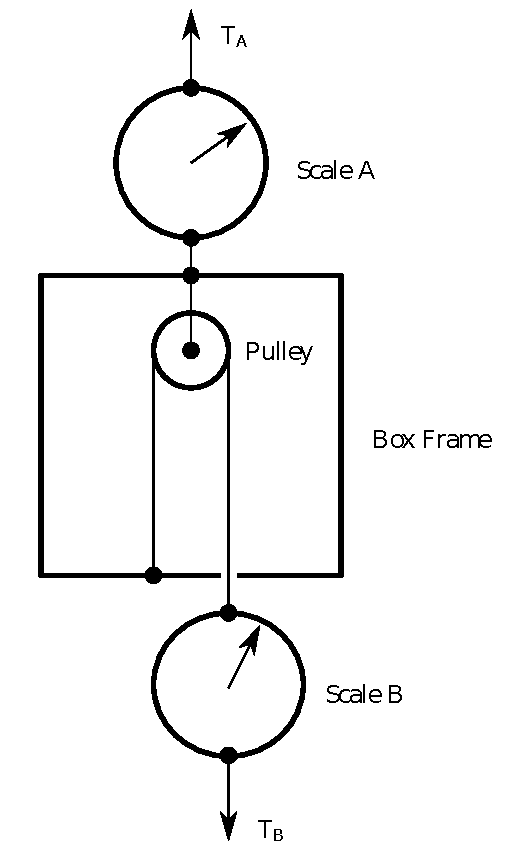
\includegraphics[keepaspectratio,scale=0.6]{Olympiad2014-Q18}
    \end{center}
    If an additional force pulls down on scale $B$ so that the reading increases to
        \SI{30}{\newton}, what will be the new reading on scale $A$?
    \begin{multicols}{3}
    \begin{choices}
        \wrongchoice{\SI{35}{\newton}}
      \correctchoice{\SI{40}{\newton}}
        \wrongchoice{\SI{45}{\newton}}
        \wrongchoice{\SI{50}{\newton}}
        \wrongchoice{\SI{60}{\newton}}
    \end{choices}
    \end{multicols}
\end{question}
}

\element{aapt}{ %% Olympiad-A3
\begin{question}{Olympiad-2014-Q19}
    A helicopter is flying horizontally at constant speed.
    A perfectly flexible uniform cable is suspended beneath the helicopter;
        air friction on the cable is not negligible.
    %% Begin Question
    Which of the following diagrams best shows the shape of the cable
        as the helicopter flies through the air to the right?
    \begin{multicols}{2}
    \begin{choices}
        %% NOTE: tikz?
        \AMCboxDimensions{down=-2cm}
        \wrongchoice{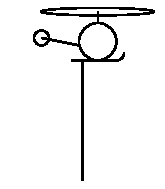
\includegraphics[keepaspectratio,scale=1.0]{Olympiad2014-Q19-A}}
      \correctchoice{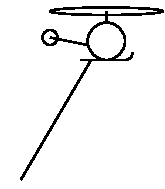
\includegraphics[keepaspectratio,scale=1.0]{Olympiad2014-Q19-B}}
        \wrongchoice{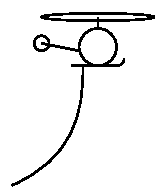
\includegraphics[keepaspectratio,scale=1.0]{Olympiad2014-Q19-C}}
        \wrongchoice{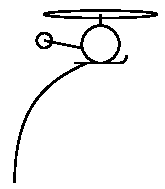
\includegraphics[keepaspectratio,scale=1.0]{Olympiad2014-Q19-D}}
        \wrongchoice{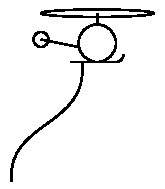
\includegraphics[keepaspectratio,scale=1.0]{Olympiad2014-Q19-E}}
    \end{choices}
    \end{multicols}
\end{question}
}


%% PhysicsOlympiad 2013
%%----------------------------------------
\newcommand{\myOlympiadThirteenQzeroFive}{
\begin{tikzpicture}
    \begin{axis}[
        axis y line=left,
        axis x line=bottom,
        axis line style={->},
        xlabel={time},
        x unit=\si{\second},
        xtick={0,2,4,6,8,10,12,14,16,18,20,22,24,26},
        ylabel={scale reading},
        y unit=\si{\kilo\gram},
        ytick={0,20,40,60,80,100,120},
        %grid=major,
        xmin=0,xmax=26,
        ymin=0,ymax=120,
        width=0.90\columnwidth,
        height=0.45\columnwidth,
    ]
    \addplot[mark=\empty] plot coordinates { (0,80) (2,80) (2,60) (4,60) (4,80) (22,80) (22,100) (24,100) (24,80) (26,80) };
    \end{axis}
\end{tikzpicture}
}

\element{aapt}{ %% Olympiad-A3
\begin{question}{Olympiad-2013-Q05}
    A student steps onto a stationary elevator and stands on a bathroom scale.
    The elevator then travels from the top of the building to the bottom.
    The student records the reading on the scale as a function of time.
    \begin{center}
        \myOlympiadThirteenQzeroFive
    \end{center}
    At what time(s) does the student have maximum downward velocity?
    \begin{choices}
        \wrongchoice{At all times between \SI{2}{\second} and \SI{4}{\second}}
        \wrongchoice{At \SI{4}{\second} only}
      \correctchoice{At all times between \SI{4}{\second} and \SI{22}{\second}}
        \wrongchoice{At \SI{22}{\second} only}
        \wrongchoice{At all times between \SI{22}{\second} and \SI{24}{\second}}
    \end{choices}
\end{question}
}

\element{aapt}{ %% Olympiad-A3
\begin{question}{Olympiad-2013-Q06}
    A student steps onto a stationary elevator and stands on a bathroom scale.
    The elevator then travels from the top of the building to the bottom.
    The student records the reading on the scale as a function of time.
    \begin{center}
        \myOlympiadThirteenQzeroFive
    \end{center}
    How tall is the building?
    \begin{multicols}{3}
    \begin{choices}
        \wrongchoice{\SI{50}{\meter}}
        \wrongchoice{\SI{80}{\meter}}
      \correctchoice{\SI{100}{\meter}}
        \wrongchoice{\SI{150}{\meter}}
        \wrongchoice{\SI{400}{\meter}}
    \end{choices}
    \end{multicols}
\end{question}
}

\element{aapt}{ %% Olympiad-A3
\begin{question}{Olympiad-2013-Q11}
    A right-triangular wooden block of mass $M$ is at rest on a table, as shown in figure.
    Two smaller wooden cubes, both with mass $m$,
        initially rest on the two sides of the larger block.
    As all contact surfaces are frictionless,
        the smaller cubes start sliding down the larger block while the block remains at rest.
    What is the normal force from the system to the table?
    \begin{center}
    \begin{tikzpicture}
        %% Triangle
        \draw (-3,0) -- (3,0);
        \draw[thick] (-2,0) -- (2,0);
        \draw[thick] (-2,0) -- ++(30:3.464);
        \draw[thick] (+2,0) -- ++(120:2);
        \node[anchor=west] at (0,0.433) {$M$};
        %% Angles
        \draw (-2,0) ++ (0:0.5) arc (0:30:0.5) node[pos=0.5,anchor=west] {$\alpha$};
        \draw (+2,0) ++ (120:0.5) arc (120:180:0.5) node[pos=0.5,anchor=east] {$\beta$};
        \draw (1,1.732) ++ (-60:0.5) -- ++(210:0.5) -- ++(120:0.5);
        %% Blocks
        \node[draw,rectangle,minimum size=1.5em,rotate=30,anchor=south] at (-0.5,0.866) {$m$};
        \node[draw,rectangle,minimum size=1.5em,rotate=30,anchor=west] at (1.5,0.866) {$m$};
    \end{tikzpicture}
    \end{center}
    \begin{choices}
        \wrongchoice{$2mg$}
        \wrongchoice{$2mg + Mg$}
      \correctchoice{$mg + Mg$}
        \wrongchoice{$Mg + mg\left(\sin\alpha + \sin\beta\right)$}
        \wrongchoice{$Mg + mg\left(\cos\alpha + \cos\beta\right)$}
    \end{choices}
\end{question}
}

\element{aapt}{ %% Olympiad-A3
\begin{question}{Olympiad-2013-Q25}
    A box with weight $W$ will slide down a \ang{30} incline at
        constant speed under the influence of gravity and friction alone.
    If instead a horizontal force $P$ is applied to the box,
        the box can be made to move up the ramp at constant speed.
    What is the magnitude of $P$?
    \begin{multicols}{2}
    \begin{choices}
        \wrongchoice{$P = \dfrac{1}{2} W$}
        \wrongchoice{$P = \dfrac{2}{\sqrt{3}} W$}
        \wrongchoice{$P = W$}
      \correctchoice{$P = \sqrt{3} W$}
        \wrongchoice{$P = 2 W$}
    \end{choices}
    \end{multicols}
\end{question}
}


%% PhysicsOlympiad 2011
%%----------------------------------------
\element{aapt}{ %% Olympiad-A3
\begin{question}{Olympiad-2012-Q11}
    As shown below, Lily is using the rope through a fixed pulley
        to move a box with constant speed $v$.
    The kinetic friction coefficient between the box and the ground is $\mu<1$;
        assume that the fixed pulley is massless and there is no friction
        between the rope and the fixed pulley.
    Then, while the box is moving,
        which of the following statements is correct?
    \begin{center}
        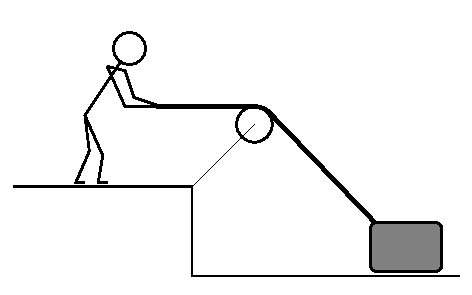
\includegraphics[keepaspectratio,scale=0.8]{Olympiad2012-Q11}
    \end{center}
    \begin{choices}
        \wrongchoice{The magnitude of the force on the rope is constant.}
      \correctchoice{The magnitude of friction between the ground and the box is decreasing.}
        \wrongchoice{The magnitude of the normal force of the ground on the box is increasing.}
        \wrongchoice{The pressure of the box on the ground is increasing.}
        \wrongchoice{The pressure of the box on the ground is constant.}
    \end{choices}
\end{question}
}



%% PhysicsOlympiad 2010
%%----------------------------------------
\element{aapt}{ %% Olympiad-A3
\begin{question}{Olympiad-2010-Q08}
    A car attempts to accelerate up a hill at an angle $\theta$ to the horizontal.
    The coefficient of static friction between the tires and
        the hill is $\mu>\tan\theta$.
    What is the maximum acceleration the car can achieve
        (in the direction upwards along the hill)?
    Neglect the rotational inertia of the wheels.
    \begin{multicols}{2}
    \begin{choices}
        \wrongchoice{$g\tan\theta$}
      \correctchoice{$g\left(\mu\cos\theta-\sin\theta\right)$}
        \wrongchoice{$g\left(\mu-\sin\theta\right)$}
        \wrongchoice{$g\mu\cos\theta$}
        \wrongchoice{$g\left(\mu\sin\theta-\cos\theta\right)$}
    \end{choices}
    \end{multicols}
\end{question}
}

\element{aapt}{ %% Olympiad-A3
\begin{question}{Olympiad-2010-Q09}
    A point object of mass $M$ hangs from the ceiling of a car
        from a massless string of length $L$.
    \begin{center}
    \begin{tikzpicture}
        %% Ceiling
        \node[anchor=south,fill,pattern=north east lines,minimum width=4cm, minimum height=0.05cm] at (0,0) {};
        \draw (-2,0) -- (2,0);
        %% Pendulum
        \draw (0,0) -- (240:5) node[pos=0.5,anchor=south east] {$L$};
        \node[draw,fill=white!90!black,thick,circle,anchor=center,minimum size=1em] at (240:5) {$M$};
        \draw[<->] (240:2) arc(240:270:2) node[pos=0.5,anchor=north] {$\theta$};
        \draw[dashed] (0,0) -- (270:5);
    \end{tikzpicture}
    \end{center}
    It is observed to make an angle $theta$ from the vertical
        as the car accelerates uniformly from rest.
    Find the acceleration of the car in terms of $\theta$, $M$, $L$, and $g$.
    \begin{multicols}{2}
    \begin{choices}
        \wrongchoice{$Mg\sin\theta$}
        \wrongchoice{$MgL\tan\theta$}
      \correctchoice{$g\tan\theta$}
        \wrongchoice{$g\cot\theta$}
        \wrongchoice{$Mg\tan\theta$}
    \end{choices}
    \end{multicols}
\end{question}
}

\element{aapt}{ %% Olympiad-A3
\begin{question}{Olympiad-2010-Q10}
    A block of mass $m_1$ is on top of a block of mass $m_2$.
    The lower block is on a horizontal surface,
        and a rope can pull horizontally on the lower block.
    The coefficient of kinetic friction for all surfaces is $\mu$.
    \begin{center}
    \begin{tikzpicture}
        %% Floor
        \node[anchor=north,fill,pattern=north east lines,minimum width=4cm, minimum height=0.05cm] at (0,0) {};
        \draw (-2,0) -- (2,0);
        %% blocks
        \node[draw,fill=white!90!black,thick,rectangle,rounded corners=1ex,minimum width=1.5cm,minimum height=0.75cm,anchor=south] (A) at (0,0) {2};
        \node[draw,fill=white!90!black,thick,rectangle,rounded corners=1ex,minimum width=0.75cm,minimum height=0.5cm,anchor=south] (B) at (A.north) {1};
        %% Force vector
        \draw[thick,->] (A.east) -- ++(0:1.5) node[pos=0.5,anchor=south] {$F$};
    \end{tikzpicture}
    \end{center}
    What is the resulting acceleration of the lower block if a
        force $F$ is applied to the rope?
    Assume that $F$ is sufficiently large so that the top block slips on the lower block.
    \begin{choices}
      \correctchoice{$a_2 = \dfrac{\left(F-\mu g\left(2m_1 + m_2\right)\right)}{m_2}$}
        \wrongchoice{$a_2 = \dfrac{\left(F-\mu g\left(m_1 + m_2\right)\right)}{m_2}$}
        \wrongchoice{$a_2 = \dfrac{\left(F-\mu g\left(m_1 + 2m_2\right)\right)}{m_2}$}
        \wrongchoice{$a_2 = \dfrac{\left(F+\mu g\left(m_1 + m_2\right)\right)}{m_2}$}
        \wrongchoice{$a_2 = \dfrac{\left(F-\mu g\left(m_2 - m_1\right)\right)}{m_2}$}
    \end{choices}
\end{question}
}


%% PhysicsOlympiad 2009
%%----------------------------------------
\element{aapt}{ %% Olympiad-A3
\begin{question}{Olympiad-2009-Q01}
    A \SI{0.3}{\kilo\gram} apple falls from rest through a height of
        \SI{40}{\centi\meter} onto a flat surface.
    Upon impact, the apple comes to rest in \SI{0.1}{\second},
        and \SI{4}{\centi\meter\squared} of the apple comes into
        contact with the surface during the impact.
    What is the average pressure exerted on the apple during the impact?
    Ignore air resistance.
    \begin{multicols}{2}
    \begin{choices}
        \wrongchoice{\SI{67 000}{\pascal}}
      \correctchoice{\SI{21 000}{\pascal}}
        \wrongchoice{\SI{6 700}{\pascal}}
        \wrongchoice{\SI{210}{\pascal}}
        \wrongchoice{\SI{67}{\pascal}}
    \end{choices}
    \end{multicols}
\end{question}
}

\element{aapt}{ %% Olympiad-A3
\begin{question}{Olympiad-2009-Q04}
    A spaceman of mass \SI{80}{\kilo\gram} is sitting in a spacecraft near the surface of the Earth.
    The spacecraft is accelerating upward at five times the acceleration due to gravity.
    What is the force of the spaceman on the spacecraft?
    \begin{multicols}{2}
    \begin{choices}
      \correctchoice{\SI{4800}{\newton}}
        \wrongchoice{\SI{4000}{\newton}}
        \wrongchoice{\SI{3200}{\newton}}
        \wrongchoice{\SI{800}{\newton}}
        \wrongchoice{\SI{400}{\newton}}
    \end{choices}
    \end{multicols}
\end{question}
}

\element{aapt}{ %% Olympiad-A3
\begin{question}{Olympiad-2009-Q15}
    A \SI{22.0}{\kilo\gram} suitcase is dragged in a straight line at a
        constant speed of \SI{1.10}{\meter\per\second} across a level airport
        floor by a student on the way to the 40th IPhO in Merida, Mexico.
    The individual pulls with a \SI{1.00e2}{\newton} force along a handle with
        makes an upward angle of \num{30.0} degrees with respect to the horizontal.
    What is the coefficient of kinetic friction between the suitcase and the floor?
    \begin{multicols}{2}
    \begin{choices}
        \wrongchoice{$\mu_k = \num{0.013}$}
        \wrongchoice{$\mu_k = \num{0.394}$}
      \correctchoice{$\mu_k = \num{0.509}$}
        \wrongchoice{$\mu_k = \num{0.866}$}
        \wrongchoice{$\mu_k = \num{1.055}$}
    \end{choices}
    \end{multicols}
\end{question}
}


%% PhysicsOlympiad 2008
%%----------------------------------------
\element{aapt}{ %% Olympiad-A3
\begin{question}{Olympiad-2008-Q08}
    Riders in a carnival ride stand with their backs against the wall
        of a circular room of diameter \SI{8.0}{\meter}.
    The room is spinning horizontally about an axis through its center
        at a rate of \SI{45}{\revolution\per\minute} when the floor drops
        so that it no longer provides any support for the riders.
    What is the minimum coefficient of static friction between the wall
        and the rider required so that the rider does not slide down the wall?
    \begin{multicols}{2}
    \begin{choices}
        \wrongchoice{\num{0.0012}}
        \wrongchoice{\num{0.056}}
      \correctchoice{\num{0.11}}
        \wrongchoice{\num{0.53}}
        \wrongchoice{\num{8.9}}
    \end{choices}
    \end{multicols}
\end{question}
}

\newcommand{\olympiadTwentyZeroEightQTen}{
\begin{tabulary}{\columnwidth}{CC}
    \toprule
    Force/(\si{\newton}) &
    acceleration/(\si{\meter\per\second\squared}) \\
    \midrule
    3.05 & 0.095 \\
    3.45 & 0.205 \\
    4.05 & 0.295 \\
    4.45 & 0.405 \\
    5.05 & 0.495 \\
    \bottomrule
\end{tabulary}
}

\element{aapt}{ %% Olympiad-A3
\begin{question}{Olympiad-2008-Q10}
    %%The following information applies to the next two problems.
    An experiment consists of pulling a heavy wooden block across a level surface with a spring force meter.
    The constant force for each try is recorded, as is the acceleration of the block.
    The data are shown below.
    \begin{center}
        \olympiadTwentyZeroEightQTen
    \end{center}
    Which is the best value for the mass of the block?
    \begin{multicols}{3}
    \begin{choices}
        \wrongchoice{\SI{3}{\kilo\gram}}
      \correctchoice{\SI{5}{\kilo\gram}}
        \wrongchoice{\SI{10}{\kilo\gram}}
        \wrongchoice{\SI{20}{\kilo\gram}}
        \wrongchoice{\SI{30}{\kilo\gram}}
    \end{choices}
    \end{multicols}
\end{question}
}

\element{aapt}{ %% Olympiad-A3
\begin{question}{Olympiad-2008-Q11}
    %%The following information applies to the next two problems.
    An experiment consists of pulling a heavy wooden block across a level surface with a spring force meter.
    The constant force for each try is recorded, as is the acceleration of the block.
    The data are shown below.
    \begin{center}
        \olympiadTwentyZeroEightQTen
    \end{center}
    Which is the best value for the coefficient of friction between the block and the surface?
    \begin{multicols}{3}
    \begin{choices}
      \correctchoice{\num{0.05}}
        \wrongchoice{\num{0.07}}
        \wrongchoice{\num{0.09}}
        \wrongchoice{\num{0.5}}
        \wrongchoice{\num{0.6}}
    \end{choices}
    \end{multicols}
\end{question}
}


%% PhysicsOlympiad 2007
%%----------------------------------------
\element{aapt}{ %% Olympiad-A3
\begin{question}{Olympiad-2007-Q05}
    A crate of toys remains at rest on a sleigh as the sleigh
        is pulled up a hill with an increasing speed.
    The crate is not fastened down to the sleigh.
    What force is responsible for the crate's increase in speed up the hill?
    \begin{choices}
      \correctchoice{the force of static friction of the sleigh on the crate}
        \wrongchoice{the contact force (normal force) of the ground on the sleigh}
        \wrongchoice{the contact force (normal force) of the sleigh on the crate}
        \wrongchoice{the gravitational force acting on the sleigh}
        \wrongchoice{no force is needed}
    \end{choices}
\end{question}
}

\element{aapt}{ %% Olympiad-A3
\begin{question}{Olympiad-2007-Q14}
    When the speed of a rear-drive car is increasing on a horizontal road,
        the direction of the frictional force on the tires is
    \begin{choices}
      \correctchoice{backward on the front tires and forward on the rear tires.}
        \wrongchoice{forward on the front tires and backward on the rear tires.}
        \wrongchoice{forward on all tires.}
        \wrongchoice{backward on all tires.}
        \wrongchoice{zero.}
    \end{choices}
\end{question}
}

\element{aapt}{ %% Olympiad-A3
\begin{question}{Olympiad-2007-Q24}
    A ball of mass $m$ is launched into the air.
    Ignore air resistance, but assume that there is a wind that
        exerts a constant force $F_0$ in the $-x$ direction.
    In terms of $F_0$ and the acceleration due to gravity $g$,
        at what angle above the positive $x$-axis must the ball be
        launched in order to come back to the point from which it was launched?
    \begin{choices}
        \wrongchoice{$\tan^{-1}\left(F_0 mg\right)$}
      \correctchoice{$\tan^{-1}\left(\frac{mg}{F_0}\right)$}
        \wrongchoice{$\sin^{-1}\left(F_0 mg\right)$}
        \wrongchoice{the angle depends on the launch speed}
        \wrongchoice{no such angle is possible}
    \end{choices}
\end{question}
}

\element{aapt}{ %% Olympiad-A3
\begin{question}{Olympiad-2007-Q26}
    A sled loaded with children starts from rest and
        slides down a snowy \ang{25} (with respect to the horizontal)
        incline traveling \SI{85}{\meter} in \SI{17}{\second}.
    Ignore air resistance.
    What is the coefficient of kinetic friction between the sled and the slope?
    \begin{multicols}{3}
    \begin{choices}
        \wrongchoice{\num{0.36}}
      \correctchoice{\num{0.40}}
        \wrongchoice{\num{0.43}}
        \wrongchoice{\num{1.00}}
        \wrongchoice{\num{2.01}}
    \end{choices}
    \end{multicols}
\end{question}
}


%% PhysicsOlympiad 2004
%%----------------------------------------
\element{aapt}{ %% Olympiad-A3
\begin{question}{Olympiad-2004-Q07}
    Two masses of \SI{5.0}{\kilo\gram} and \SI{7.0}{\kilo\gram} are originally at rest on a frictionless surface.
    The masses are connected by a light cord.
    \begin{center}
    \begin{tikzpicture}
        %% floor
        \draw (-3,0) -- (3,0);
        \node[anchor=north,fill,pattern=north east lines,minimum width=6cm,minimum height=0.1cm] at (0,0) {};
        %% blocks
        \node[draw,anchor=south,minimum size=1cm] (L) at (-2,0) {\SI{5}{\kilo\gram}};
        \node[draw,anchor=south,minimum size=1.2cm] (R) at (+1,0) {\SI{7}{\kilo\gram}};
        %% Force
        \draw[thick,->] (R.east) -- ++(0:2) node[pos=0.5,anchor=south] {\SI{30}{\newton}};
        \draw[thick] (R.west) -- ++(180:1.9);
    \end{tikzpicture}
    \end{center}
    A second cord is attached to the \SI{7.0}{\kilo\gram} mass and pulled with a horizontal force of \SI{30}{\newton}.
    What is the tension in the cord that connects the two masses?
    \begin{multicols}{3}
    \begin{choices}
        \wrongchoice{\SI{5}{\newton}}
        \wrongchoice{\SI{7}{\newton}}
      \correctchoice{\SI{12.5}{\newton}}
        \wrongchoice{\SI{17.5}{\newton}}
        \wrongchoice{\SI{30}{\newton}}
    \end{choices}
    \end{multicols}
\end{question}
}

\element{aapt}{ %% Olympiad-A3
\begin{question}{Olympiad-2004-Q08}
    Two masses are connected by a light cord which is looped over a light frictionless pulley.
    \begin{center}
    \begin{tikzpicture}
        %% Ceiling
        \node[anchor=south,fill,pattern=north east lines,minimum width=4cm, minimum height=0.05cm] at (0,0) {};
        \draw[thick] (-2,0) -- (2,0);
        %% pulley
        \draw (0,-1) circle (0.75cm);
        \draw[fill=white!50!black] (-0.2,0) -- (-0.1,-1.05) arc (200:340:0.1) -- (0.2,0) --cycle;
        \draw[fill] (0,-1) circle (1pt);
        %% masses
        \node[minimum size=1.0cm,draw,fill=white!90!black] (L) at (-0.75,-3) {\SI{3}{\kilo\gram}};
        \node[minimum size=1.3cm,draw,fill=white!90!black] (R) at (+0.75,-4) {\SI{5}{\kilo\gram}};
        %% rope
        \draw (R.north) -- (+0.75,-1);
        \draw (L.north) -- (-0.75,-1);
    \end{tikzpicture}
    \end{center}
    If one mass is \SI{3.0}{\kilo\gram} and the second mass is \SI{5.0}{\kilo\gram},
        what is the downward acceleration of the heavier mass?
    Assume air resistance is negligible.
    \begin{multicols}{3}
    \begin{choices}
        \wrongchoice{\SI{9.8}{\meter\per\second\squared}}
        \wrongchoice{\SI{8.4}{\meter\per\second\squared}}
        \wrongchoice{\SI{6.3}{\meter\per\second\squared}}
        \wrongchoice{\SI{3.8}{\meter\per\second\squared}}
      \correctchoice{\SI{2.5}{\meter\per\second\squared}}
    \end{choices}
    \end{multicols}
\end{question}
}


%% PhysicsOlympiad 2003
%%----------------------------------------
\element{aapt}{ %% Olympiad-A3
\begin{question}{Olympiad-2003-Q04}
    A skydiver is falling at terminal velocity before opening her parachute.
    After opening her parachute, she falls at a much smaller terminal velocity.
    How does the total upward force before she opens her parachute compare to the total upward force after she opens her parachute?
    \begin{choices}
        \wrongchoice{the ratio of the forces is equal to the ratio of the velocities}
        \wrongchoice{the ratio of the forces is equal to the inverse ratio of the velocities}
        \wrongchoice{the upward force with the parachute will depend on the size of the parachute}
        \wrongchoice{the upward force before the parachute will be greater because of the greater velocity}
      \correctchoice{the upward force in both cases must be the same}
    \end{choices}
\end{question}
}

\newcommand{\OlympiadTwentyZeroThreeQEight}{
\begin{tikzpicture}[font=\small]
    %% Ceiling
    \node[anchor=south,fill,pattern=north east lines,minimum width=4cm, minimum height=0.05cm] at (0,0) {};
    \draw[thick] (-2,0) -- (2,0);
    %% pulley
    \draw (0,-1) circle (0.75cm);
    \draw[fill=white!70!black] (-0.2,0) -- (-0.15,-1.05) arc (190:350:0.15) -- (0.2,0) --cycle;
    \draw[fill] (0,-1) circle (1.5pt);
    %% masses
    \node[minimum size=1.2cm,draw,fill=white!90!black] (L) at (-0.75,-4) {$M_1$};
    \node[minimum size=1cm,draw,fill=white!90!black] (R) at (+0.75,-3) {$M_2$};
    %% rope
    \draw (R.north) -- (+0.75,-1);
    \draw (L.north) -- (-0.75,-1);
\end{tikzpicture}
}

\element{aapt}{ %% Olympiad-A3
\begin{question}{Olympiad-2003-Q08A}
    Two weights are connected by a massless string which passes over a massless pulley.
    \begin{center}
        \OlympiadTwentyZeroThreeQEight
    \end{center}
    Which value of $M_1$ and $M_2$ will result in the largest magntidue of acceleration?
    \begin{choices}
      \correctchoice{$M_1=\SI{2}{\kilo\gram}$, $M_2=\SI{1}{\kilo\gram}$}
        \wrongchoice{$M_1=\SI{4}{\kilo\gram}$, $M_2=\SI{3}{\kilo\gram}$}
        \wrongchoice{$M_1=\SI{5}{\kilo\gram}$, $M_2=\SI{3}{\kilo\gram}$}
        \wrongchoice{$M_1=\SI{8}{\kilo\gram}$, $M_2=\SI{5}{\kilo\gram}$}
        \wrongchoice{$M_1=\SI{10}{\kilo\gram}$, $M_2=\SI{6}{\kilo\gram}$}
    \end{choices}
\end{question}
}


%% PhysicsOlympiad 2000
%%----------------------------------------
\element{aapt}{ %% Olympiad-A3
\begin{question}{olympiad-2000-q05}
    An object originally traveling at a velocity, $v_0$,
        is accelerated to a velocity, $v$, in a time, $t$, by a constant force, $F$.
    What would be the mass of the object?
    \begin{multicols}{3}
    \begin{choices}
        \wrongchoice{$\dfrac{v-v_0}{Ft}$}
      \correctchoice{$\dfrac{Ft}{v-v_0}$}
        \wrongchoice{$\dfrac{F\left(v-v_0\right)}{t}$}
        \wrongchoice{$\dfrac{F}{vt}$}
        \wrongchoice{$\dfrac{F}{v_0t}$}
    \end{choices}
    \end{multicols}
\end{question}
}

\element{aapt}{ %% Olympiad-A3
\begin{question}{olympiad-2000-q13}
    A block is sliding frictionlessly up a plane inclined at an angle of \ang{45} to the horizontal.
    \begin{center}
    \begin{tikzpicture}
        %% incline and angle
        \draw[thick] (0,0) -- ++(45:6);
        \draw (0,0) -- ++(0:4.24);
        \draw[<->] (1.5,0) arc (0:45:1.5) node[pos=0.5,anchor=west] {\ang{45}};
        %% Block
        \node[draw,fill=white!90!black,minimum size=1cm,anchor=south,rotate=45] (A) at (45:3) {};
        \draw[thick,->] (A.east) -- ++(45:1.5) node[pos=0.5,anchor=south,rotate=45] {\SI{25}{\meter\per\second}};
    \end{tikzpicture}
    \end{center}
    If at a given time the block's velocity is \SI{+25}{\meter\per\second} in the upward direction what is the velocity of the block \SI{4.0}{\second} later?
    \begin{multicols}{3}
    \begin{choices}
        \wrongchoice{\SI{+64.2}{\meter\per\second}}
        \wrongchoice{\SI{+53.3}{\meter\per\second}}
        \wrongchoice{\SI{+28.3}{\meter\per\second}}
        \wrongchoice{\SI{+7.1}{\meter\per\second}}
      \correctchoice{\SI{-2.7}{\meter\per\second}}
    \end{choices}
    \end{multicols}
\end{question}
}

\element{aapt}{ %% Olympiad-A3
\begin{question}{olympiad-2000-q14}
    Three blocks ($m_1$, $m_2$ and $m_3$) are slid at constant velocity across a rough surface as shown below.
    \begin{center}
    \begin{tikzpicture}
        %% Ground
        \draw (-5,0) -- (2,0);
        \node[anchor=north,fill,pattern=north east lines,minimum width=7cm, minimum height=0.1cm] at (-1.5,0) {};
        %% Three Blocks
        \node[draw,minimum size=1.5cm,fill=white!90!black,anchor=south east] (A) at (0,0) {$m_1$};
        \node[draw,minimum size=1.2cm,fill=white!90!black,anchor=south east] (B) at (A.south west) {$m_2$};
        \node[draw,minimum size=1.0cm,fill=white!90!black,anchor=south east] (C) at (B.south west) {$m_3$};
        %% Force
        \draw[very thick,<-] (A.east) -- ++(0:2) node[pos=0.5,anchor=south] {$F$};
    \end{tikzpicture}
    \end{center}
    The coefficient of kinetic friction between each block and the surface is $\mu$.
    What would be the force of $m_1$ on $m_2$?
    \begin{multicols}{2}
    \begin{choices}
        \wrongchoice{$F$}
        \wrongchoice{$F -\left(m_2 - m_3\right) g\mu$}
      \correctchoice{$\left(m_2 + m_3\right) g\mu$}
        \wrongchoice{$m_1g\mu - \left(m_2 + m_3\right) g\mu$}
        \wrongchoice{$\left(m_1 + m_2 + m_3\right) g\mu$}
    \end{choices}
    \end{multicols}
\end{question}
}

\element{aapt}{ %% Olympiad-A3
\begin{question}{olympiad-2000-q17}
    %% Questions 17 and 18 refer to the situation shown in the accompanying diagram.
    Two \SI{5}{\kilo\gram} masses are attached to opposite ends of a long massless cord which passes tautly over a massless frictionless pulley.
    The upper mass is initially held at rest on a table \SI{50}{\centi\meter} from the pulley.
    The coefficient of kinetic friction between this mass and the table is \num{0.20}.
    \begin{center}
    \begin{tikzpicture}
        %% Floor
        \draw[very thick] (-3,0) -- (0,0) -- (0,-2);
        %% Mass
        \node[draw,fill=white!90!black,rectangle,rounded corners=1ex,minimum size=1.0cm,anchor=south] (A) at (-2,0) {\SI{5.0}{\kilo\gram}};
        \node[draw,fill=white!90!black,rectangle,rounded corners=1ex,minimum size=1.0cm,anchor=north] (B) at (1,-1) {\SI{5.0}{\kilo\gram}};
        %% Rope and Pully
        \draw[thick] (A.south east) ++(90:0.5) -- (0.75,0.5) arc(90:0:0.25) -- (B.north);
        \draw[thick,fill=white!90!black] (0.75,0.25) circle (0.25);
        \draw[thick,fill=white] (0,0) -- (0.75,0.35) arc (90:-60:0.1) -- (0,-0.5) -- cycle;
        \draw[fill] (0.75,0.25) circle (1pt);
    \end{tikzpicture}
    \end{center}
    %% start question
    When the system is released, its resulting acceleration is closest to which of the following:
    \begin{multicols}{3}
    \begin{choices}
        \wrongchoice{\SI{9.8}{\meter\per\second\squared}}
        \wrongchoice{\SI{7.8}{\meter\per\second\squared}}
        \wrongchoice{\SI{4.9}{\meter\per\second\squared}}
      \correctchoice{\SI{3.9}{\meter\per\second\squared}}
        \wrongchoice{\SI{1.9}{\meter\per\second\squared}}
    \end{choices}
    \end{multicols}
\end{question}
}


%% PhysicsOlympiad 1999
%%----------------------------------------
\element{aapt}{ %% Olympiad-A3
\begin{question}{olympiad-1999-q02}
    Hercules and Ajax horizontally push in the same direction on a \SI{1200}{\kilo\gram} crate.
    Hercules pushes with a force of \SI{500}{\newton} and Ajax pushes with a force of \SI{300}{\newton}.
    If a frictional force provides \SI{200}{\newton} of resistance,
        what is the acceleration of the crate?
    \begin{multicols}{3}
    \begin{choices}
        \wrongchoice{\SI{1.3}{\meter\per\second\squared}}
        \wrongchoice{\SI{1.0}{\meter\per\second\squared}}
        \wrongchoice{\SI{0.87}{\meter\per\second\squared}}
        \wrongchoice{\SI{0.75}{\meter\per\second\squared}}
      \correctchoice{\SI{0.5}{\meter\per\second\squared}}
    \end{choices}
    \end{multicols}
\end{question}
}

\element{aapt}{ %% Olympiad-A3
\begin{question}{olympiad-1999-q07}
    If a net force $F$ applied to an object of mass $m$ will produce an acceleration of $a$,
        what is the mass of a second object which accelerates at $5a$ when acted upon by a net force of $2F$?
    \begin{multicols}{3}
    \begin{choices}
      \correctchoice{$\dfrac{2}{5} m$}
        \wrongchoice{$2 m$}
        \wrongchoice{$\dfrac{5}{2} m$}
        \wrongchoice{$5m$}
        \wrongchoice{$10m$}
    \end{choices}
    \end{multicols}
\end{question}
}

\element{aapt}{ %% Olympiad-A3
\begin{question}{olympiad-1999-q15}
    A \SI{4.0}{\kilo\gram} mass is attached to one end of a rope \SI{2}{\meter} long.
    If the mass is swung in a vertical circle from the free end of the rope,
        what is the tension in the rope when the mass is at its highest point if it is moving with a speed of \SI{5}{\meter\per\second}?
    \begin{multicols}{3}
    \begin{choices}
        \wrongchoice{\SI{5.4}{\newton}}
      \correctchoice{\SI{10.8}{\newton}}
        \wrongchoice{\SI{21.6}{\newton}}
        \wrongchoice{\SI{50}{\newton}}
        \wrongchoice{\SI{65.4}{\newton}}
    \end{choices}
    \end{multicols}
\end{question}
}


%% PhysicsOlympiad 1998
%%----------------------------------------
\element{aapt}{ %% Olympiad-A3
\begin{question}{olympiad-1998-q07}
    Two identical blocks of weight $W$ are placed one on top of the other as shown below.
    \begin{center}
    \begin{tikzpicture}
        %% Ground
        \draw (0,0) -- (-6,0);
        \node[anchor=north,fill,pattern=north east lines,minimum width=6cm, minimum height=0.05cm] at (-3,0) {};
        %% Wall
        \draw (0,0) -- (0,3);
        \node[anchor=west,fill,pattern=north east lines,minimum width=0.1cm, minimum height=3.2cm] at (0,+1.4) {};
        %% block
        \node[fill=white!90!black,rounded corners=1ex,minimum width=2cm,minimum height=1cm,draw,anchor=south] (B) at (-3,0) {$m$};
        \node[fill=white!90!black,rounded corners=1ex,minimum width=2cm,minimum height=1cm,draw,anchor=south] (T) at (B.north) {$m$};
        %% force
        \draw[very thick,->] (B.west) -- ++(180:1.5) node[pos=0.5,anchor=south] {$F$};
        \draw[very thick] (T.east) -- ++(0:2);
    \end{tikzpicture}
    \end{center}
    The upper block is tied to the wall.
    The lower block is pulled to the right with a force $F$.
    The coefficient of static friction between all surfaces in contact is $\mu$.
    What is the largest force $F$ that can be exerted before the lower block starts to slip?
    \begin{multicols}{3}
    \begin{choices}
        \wrongchoice{$\mu W$}
        \wrongchoice{$\dfrac{3}{2} \mu W$}
        \wrongchoice{$2 \mu W$}
        \wrongchoice{$\dfrac{5}{2} \mu W$}
      \correctchoice{$3 \mu W$}
    \end{choices}
    \end{multicols}
\end{question}
}

\element{aapt}{ %% Olympiad-A3
\begin{question}{olympiad-1998-q08}
    An object placed on an equal arm balance requires \SI{12}{\kilo\gram} to balance it.
    When placed on a spring scale, the scale reads \SI{120}{\newton}.
    Everything (balance, scale, set of masses, and the object)
        is now transported to the moon where the gravitational force is one-sixth that on Earth.
    The new readings of the balance and the spring scale (respectively) are:
    \begin{multicols}{2}
    \begin{choices}
      \correctchoice{\SI{12}{\kilo\gram}, \SI{20}{\newton}}
        \wrongchoice{\SI{12}{\kilo\gram}, \SI{120}{\newton}}
        \wrongchoice{\SI{12}{\kilo\gram}, \SI{720}{\newton}}
        \wrongchoice{\SI{2}{\kilo\gram}, \SI{20}{\newton}}
        \wrongchoice{\SI{2}{\kilo\gram}, \SI{120}{\newton}}
    \end{choices}
    \end{multicols}
\end{question}
}


%% PhysicsOlympiad 1997
%%----------------------------------------
\element{aapt}{ %% Olympiad-A3
\begin{question}{olympiad-1997-q04}
    A force $F$ is used to hold a block of mass $m$ on an incline as shown in the diagram.
    \begin{center}
    \begin{tikzpicture}
        %% incline
        \draw[thick] (0,0) -- (30:6);
        \draw[thick,dashed] (0,0) -- (0:5.196);
        \draw[<->] (1.5,0) arc (0:30:1.5) node[pos=0.5,anchor=west] {$\theta$};
        %% block
        \node[draw,anchor=south,minimum size=1cm,rotate=30,fill=white!90!black] (A) at (30:4) {};
        %% force
        \draw[very thick,<-] (A.north) -- ++(120:1) node[pos=0.5,anchor=west] {$F$};
    \end{tikzpicture}
    \end{center}
    The plane makes an angle of $\theta$ with the horizontal and $F$ is perpendicular to the plane.
    The coefficient of friction between the plane and the block is $\mu$.
    What is the minimum force, $F$, necessary to keep the block at rest?
    \begin{multicols}{2}
    \begin{choices}
        \wrongchoice{$\mu mg$}
        \wrongchoice{$mg \cos\theta$}
        \wrongchoice{$mg \sin\theta$}
        \wrongchoice{$\dfrac{mg}{\mu} \sin\theta$}
      \correctchoice{$\dfrac{mg}{\mu} \left(\sin\theta-\mu\cos\theta\right)$}
    \end{choices}
    \end{multicols}
\end{question}
}

\element{aapt}{ %% Olympiad-A3
\begin{question}{olympiad-1997-q05}
    You hold a rubber ball in your hand.
    The Newton's third law companion force to the force of gravity on the ball is the force exerted by the:
    \begin{choices}
      \correctchoice{ball on the Earth.}
        \wrongchoice{ball on the hand.}
        \wrongchoice{hand on the ball.}
        \wrongchoice{Earth on the ball.}
        \wrongchoice{Earth on your hand.}
    \end{choices}
\end{question}
}

\element{aapt}{ %% Olympiad-A3
\begin{question}{olympiad-1997-q06}
    A ball of mass $m$ is fastened to a string.
    The ball swings in a vertical circle of radius $R$ with the other end of the string held fixed.
    Neglecting air resistance,
        the difference between the string's tension at the bottom of the circle and at the top of the circle is:
    \begin{multicols}{3}
    \begin{choices}
        \wrongchoice{$mg$}
        \wrongchoice{$2 mg$}
        \wrongchoice{$4 mg$}
      \correctchoice{$6 mg$}
        \wrongchoice{$8 mg$}
    \end{choices}
    \end{multicols}
\end{question}
}


%% PhysicsOlympiad 1996
%%----------------------------------------
\element{aapt}{ %% Olympiad-A3
\begin{question}{olympiad-1996-q05}
    What is the tension $T$ in the rope if the \SI{10}{\newton} weight is moving upward with constant velocity?
    \begin{center}
    \begin{tikzpicture}
        %% Ceiling
        \node[anchor=south,fill,pattern=north east lines,minimum width=6cm, minimum height=0.05cm] at (-1,0) {};
        \draw (-4,0) -- (2,0);
        %% Rope
        \draw[very thick,->] (+1.0,0) -- (+1,-3) arc(0:-180:0.5) -- (0,-1) arc(0:135:0.5) -- ++(225:3.5) node[pos=1.0,anchor=south,yshift=0.05cm] {$T$};
        \draw[dashed] (-0.5,-0.5) ++(-0.3535,-0.1464) ++(225:3) -- ++(0:2);
        \draw[thick,<->] (-0.5,-0.5) ++(-0.3535,-0.1464) ++(225:3) ++(0:1.5) arc(0:45:1.5) node[pos=0.5,anchor=west] {\ang{45}};
        %% first pulley
        \draw[thick] (-0.5,-1) circle (0.5);
        \draw[fill=white!90!black] (-0.8,0) -- (-0.7,-1.1) arc(190:350:0.2) -- (-0.2,0) --cycle;
        \draw[fill] (-0.5,-1) circle (1.5pt);
        %% second pulley
        \draw[thick] (0.5,-3) circle (0.50);
        \draw[fill] (0.5,-3) circle (1.5pt);
        %% Masses
        \node[draw,fill=white!90!black,rectangle,rounded corners=1ex,minimum size=1.2cm,anchor=north] (B) at (0.5,-4) {\SI{10}{\newton}};
        \draw[thick] (B.north) -- (0.5,-3);
    \end{tikzpicture}
    \end{center}
    \begin{multicols}{3}
    \begin{choices}
        \wrongchoice{\SI{3.5}{\newton}}
      \correctchoice{\SI{5.0}{\newton}}
        \wrongchoice{\SI{7.1}{\newton}}
        \wrongchoice{\SI{10}{\newton}}
        \wrongchoice{\SI{14}{\newton}}
    \end{choices}
    \end{multicols}
\end{question}
}

\element{aapt}{ %% Olympiad-A3
\begin{question}{olympiad-1996-q06}
    As shown below,
        two blocks with masses $m$ and $M$ ($M>m$) are pushed by a force $F$ in both Case I and Case II.
    \begin{center}
    \begin{tikzpicture}
        %% Ground
        \node[anchor=north,fill,pattern=north east lines,minimum width=8cm, minimum height=0.05cm] at (0,0) {};
        \draw (-4,0) -- (4,0);
        %% Case I
        \begin{scope}[xshift=-1.75cm]
            \node[anchor=south east,draw,minimum size=1.4cm] (A1) at (0,0) {$M$};
            \node[anchor=south west,draw,minimum size=1.0cm] (B1) at (0,0) {$m$};
            \draw[ultra thick,<-] (A1.west) -- ++(180:1) node[pos=0.5,anchor=south] {$F$};
            \node[anchor=south] at (A1.north) {Case I};
        \end{scope}
        %% Case II
        \begin{scope}[xshift=+1.75cm]
            \node[anchor=south east,draw,minimum size=1.4cm] (A2) at (0,0) {$M$};
            \node[anchor=south west,draw,minimum size=1.0cm] (B2) at (0,0) {$m$};
            \draw[ultra thick,<-] (B2.east) -- ++(0:1) node[pos=0.5,anchor=south] {$F$};
            \node[anchor=south] at (A2.north) {Case II};
        \end{scope}
    \end{tikzpicture}
    \end{center}
    The surface is horizontal and frictionless.
    Let $R_{I}$ be the force that $m$ exerts on $M$ in case I and $R_{II}$ be the force that $m$ exerts on $M$ in case II.
    Which of the following statements is true?
    \begin{choices}
        \wrongchoice{$R_{I} = R_{II} = 0$}
        \wrongchoice{$R_{I} = R_{II}$ and is not equal to zero or $F$.}
        \wrongchoice{$R_{I} = R_{II} = F$}
      \correctchoice{$R_{I} < R_{II}$}
        \wrongchoice{$R_{I} > R_{II}$}
    \end{choices}
\end{question}
}

\element{aapt}{ %% Olympiad-A3
\begin{question}{olympiad-1996-q07}
    Two blocks, with masses \SI{17}{\kilo\gram} and \SI{15}{\kilo\gram},
        are connected by a light string that passes over a frictionless pulley of negligible mass as shown.
    \begin{center}
    \begin{tikzpicture}
        %% Ground
        \node[anchor=north,fill,pattern=north east lines,minimum width=8cm, minimum height=0.05cm] at (-1,0) {};
        \draw (-5,0) -- (3,0);
        %% Triangle
        \draw (-4,0) -- ++(45:5.657);
        \draw (+2.309,0) -- ++(120:4.619);
        %% angles
        \draw[<->] (-3,0) arc (0:45:1) node[pos=0.5,anchor=west] {\ang{45}};
        \draw[<->] (+1.309,0) arc (180:120:1) node[pos=0.5,anchor=east] {\ang{60}};
        %% pulley
        \draw[] (0,4.4) circle (0.25cm);
        \draw[fill] (0,4.4) circle (1pt);
        \draw[fill] (0,4.0) circle (1pt);
        \draw[very thick] (0,4.0) -- (0,4.4);
        \draw[thick] (0,4.65) arc(90:135:0.25) -- ++(225:2.85) node[pos=0.6,anchor=south,rotate=45] {$T_2$};
        \draw[thick] (0,4.65) arc(90:45:0.25) -- ++(-60:2.5) node[pos=0.6,anchor=south,rotate=-60] {$T_1$};
        %% left and right block
        \path (-4,0) ++(45:2.5) node[draw,rotate=45,anchor=south,minimum size=1.2cm] {\SI{17}{\kilo\gram}};
        \path (+2.309,0) -- ++(120:2) node[draw,rotate=-60,anchor=south,minimum size=1cm] {\SI{15}{\kilo\gram}};
    \end{tikzpicture}
    \end{center}
    The surfaces of the planes are frictionless.
    The blocks are released from rest.
    $T_1$ and $T_2$ are the tensions in the strings.
    Which of the following statements is correct?
    \begin{choices}
      \correctchoice{The \SI{15}{\kilo\gram} block accelerates down the plane.}
        \wrongchoice{The \SI{17}{\kilo\gram} block accelerates down the plane.}
        \wrongchoice{Both blocks remain at rest.}
        \wrongchoice{$T_1 > T_2$}
        \wrongchoice{$T_1 < T_2$}
    \end{choices}
\end{question}
}

\element{aapt}{ %% Olympiad-A3
\begin{question}{olympiad-1996-q08}
    A small block of mass $m$ starts from rest at the top of a globe of radius $R$.
    \begin{center}
    \begin{tikzpicture}
        %% globe
        \draw (0,0) circle (2cm);
        \draw[thick,->] (0,0) -- (41:2) node[anchor=north,pos=0.6] {$R$};
        \draw[dashed] (0,0) -- (90:2);
        \draw[<->] (0,1) arc(90:41:1) node[pos=0.5,anchor=south] {$\theta$};
        %% top block
        \node[anchor=south,draw,fill=white!90!black,minimum size=0.33cm] at (0,2) {};
        %% bottom block
        \node[anchor=south,draw,rotate=-48,minimum size=0.33cm] at (41:2) {};
    \end{tikzpicture}
    \end{center}
    At what angle $\theta$ does it slide off the surface of the globe?
    Assume the system is frictionless.
    \begin{multicols}{2}
    \begin{choices}
        \wrongchoice{$\theta = \ang{0}$}
        \wrongchoice{$\theta = \cos^{-1}\left(\dfrac{1}{3}\right)$}
      \correctchoice{$\theta = \cos^{-1}\left(\dfrac{2}{3}\right)$}
        \wrongchoice{$\theta = \ang{60}$}
        \wrongchoice{$\theta = \ang{90}$}
        %% added distractor ?
        %\wrongchoice{$\theta = \cos^{-1}\left(\dfrac{1}{2}\right)$}
    \end{choices}
    \end{multicols}
\end{question}
}

\element{aapt}{ %% Olympiad-A3
\begin{questionmult}{olympiad-1996-q09}
    An object with mass $m$ and initial velocity $v$ is brought to rest by a constant force $F$ acting for a time $t$ and through a distance $d$.
    %Possible expressions for the magnitude of the force $F$ are:
    Which of these give(s) the correct expression for the magnitude of the force $F$?
    \begin{multicols}{3}
    \begin{choices}
      \correctchoice{$\dfrac{mv^2}{2d}$}
      \correctchoice{$\dfrac{2md}{t^2}$}
      \correctchoice{$\dfrac{mv}{t}$}
    \end{choices}
    \end{multicols}
\end{questionmult}
}


%% PhysicsOlympiad 1995
%%----------------------------------------
\element{aapt}{ %% Olympiad-A3
\begin{question}{olympiad-1995-q03}
    Three blocks---1, 2, and 3---rest on a horizontal frictionless surface,
        as shown in the accompanying figure.
    Each block has a mass $m$, and the blocks are connected by massless strings.
    Block 3 is pulled to the right by a force $F$.
    \begin{center}
    \begin{tikzpicture}
        %% Floor
        \node[anchor=north,fill,pattern=north east lines,minimum width=8cm, minimum height=0.05cm] at (-1.5,0) {};
        \draw (-5.5,0) -- (2.5,0);
        %% Blocks
        \node[anchor=south,minimum size=1cm,draw,fill=white!90!black] (A) at (0,0) {$m$};
        \node[anchor=south,minimum size=1cm,draw,fill=white!90!black] (B) at (-2,0) {$m$};
        \node[anchor=south,minimum size=1cm,draw,fill=white!90!black] (C) at (-4,0) {$m$};
        %% Labels
        \node[anchor=south] at (A.north) {3};
        \node[anchor=south] at (B.north) {2};
        \node[anchor=south] at (C.north) {1};
        %% Strings
        \draw[thick] (A.west) -- (B.east);
        \draw[thick] (B.west) -- (C.east);
        %% Force
        \draw[thick,->] (A.east) -- ++(0:1.5cm) node[pos=0.5,anchor=south] {$F$};
    \end{tikzpicture}
    \end{center}
    The resultant force on block 2 is:
    \begin{multicols}{3}
    \begin{choices}
        \wrongchoice{zero}
      \correctchoice{$\dfrac{F}{3}$}
        \wrongchoice{$\dfrac{F}{2}$}
        \wrongchoice{$\dfrac{2F}{3}$}
        \wrongchoice{$F$}
    \end{choices}
    \end{multicols}
\end{question}
}

\element{aapt}{ %% Olympiad-A3
\begin{question}{olympiad-1995-q04}
    Which solid vector in the accompanying figures best represents the acceleration of a pendulum mass at an intermediate point in its swing?
    \begin{multicols}{2}
    \begin{choices}
        \AMCboxDimensions{down=-1cm}
        \wrongchoice{
            \begin{tikzpicture}
                \draw[dashed,white!90!black] (-1.5,-2.75) rectangle (1.5,0.2);
                %% string
                \draw (0,0) -- (300:2);
                %% path
                \draw[thick,white!80!black,latex-latex] (225:2) arc(225:315:2);
                %% arrows
                \draw[thick,-latex] (300:2) -- ++(210:1);
                %% bob
                \draw[fill=white!80!black] (300:2) circle (5pt);
            \end{tikzpicture}
        }
        \wrongchoice{
            \begin{tikzpicture}
                \draw[dashed,white!90!black] (-1.5,-2.75) rectangle (1.5,0.2);
                %% string
                \draw (0,0) -- (300:2);
                %% path
                \draw[thick,white!80!black,latex-latex] (225:2) arc(225:315:2);
                %% arrows
                \draw[thick,-latex] (300:2) -- ++(120:1);
                %% bob
                \draw[fill=white!80!black] (300:2) circle (5pt);
            \end{tikzpicture}
        }
        \wrongchoice{
            \begin{tikzpicture}
                \draw[dashed,white!90!black] (-1.5,-2.75) rectangle (1.5,0.2);
                %% string
                \draw (0,0) -- (300:2);
                %% path
                \draw[thick,white!80!black,latex-latex] (225:2) arc(225:315:2);
                %% arrows
                \draw[thick,-latex] (300:2) -- ++(270:1);
                %% bob
                \draw[fill=white!80!black] (300:2) circle (5pt);
            \end{tikzpicture}
        }
        %% ANS is D
        \correctchoice{
            \begin{tikzpicture}
                \draw[dashed,white!90!black] (-1.5,-2.75) rectangle (1.5,0.2);
                %% string
                \draw (0,0) -- (300:2);
                %% path
                \draw[thick,white!80!black,latex-latex] (225:2) arc(225:315:2);
                %% arrows
                \draw[thick,-latex] (300:2) -- ++(160:1);
                %% bob
                \draw[fill=white!80!black] (300:2) circle (5pt);
            \end{tikzpicture}
        }
        \wrongchoice{
            \begin{tikzpicture}
                \draw[dashed,white!90!black] (-1.5,-2.75) rectangle (1.5,0.2);
                %% string
                \draw (0,0) -- (300:2);
                %% path
                \draw[thick,white!80!black,latex-latex] (225:2) arc(225:315:2);
                %% arrows
                \draw[thick,-latex] (300:2) -- ++(210:1);
                %% bob
                \draw[fill=white!80!black] (300:2) circle (5pt);
            \end{tikzpicture}
        }
    \end{choices}
    \end{multicols}
\end{question}
}

\element{aapt}{ %% Olympiad-A3
\begin{question}{olympiad-1995-q06}
    Two identical masses $m$ are connected to a massless string which is hung over two frictionless pulleys as shown.
    \begin{center}
    \begin{tikzpicture}
        %% Ceiling
        \node[anchor=south,fill,pattern=north east lines,minimum width=8cm, minimum height=0.05cm] at (0,0) {};
        \draw (-4,0) -- (4,0);
        %% Mass Left
        \node[draw,anchor=north,minimum size=1cm,fill=white!90!black,rounded corners=0.5ex] (A) at (-2.5,-2.5) {$m$};
        %% Mass Right
        \node[draw,anchor=north,minimum size=1cm,fill=white!90!black,rounded corners=0.5ex] (B) at (+2.5,-2.5) {$m$};
        %% Rope
        \draw[very thick] (A.north) -- (-2.5,-1) arc(180:90:0.5) -- (+2,-0.5) arc(90:0:0.5) -- (B.north);
        %% Pulley Left
        \draw (-2,-1) circle (0.5cm);
        \draw[fill=white!90!black] (-2.2,0) -- (-2.1,-1.1) arc(190:350:0.1) -- (-1.8,0) -- cycle;
        \draw[fill] (-2,-1) circle (1pt);
        %% Pulley Right
        \draw (+2,-1) circle (0.5cm);
        \draw[fill=white!90!black] (+1.8,0) -- (+1.9,-1.1) arc(190:350:0.1) -- (+2.2,0) -- cycle;
        \draw[fill] (+2,-1) circle (1pt);
    \end{tikzpicture}
    \end{center}
    If everything is at rest,
        what is the tension in the cord?
    \begin{choices}
        \wrongchoice{Less than $mg$.}
      \correctchoice{Exactly $mg$.}
        \wrongchoice{More than $mg$ but less than $2mg$.}
        \wrongchoice{Exactly $2mg$.}
        \wrongchoice{More than $2mg$.}
    \end{choices}
\end{question}
}

\element{aapt}{ %% Olympiad-A3
\begin{question}{olympiad-1995-q11}
    The driver of a \SI{1000}{\kilo\gram} car tries to turn through a circle of radius \SI{100}{\meter} on an unbanked curve at a speed of \SI{10}{\meter\per\second}.
    The maximum frictional force between the tires and the slippery road is \SI{900}{\newton}.
    The car will:
    \begin{choices}
        \wrongchoice{Slide into the inside of the curve.}
        \wrongchoice{Make the turn.}
        \wrongchoice{Slow down due to the centrifugal force.}
        \wrongchoice{Make the turn only if it speeds up.}
      \correctchoice{Slide off to the outside of the curve.}
    \end{choices}
\end{question}
}


%% PhysicsOlympiad 1994
%%----------------------------------------
\element{aapt}{ %% Olympiad-A3
\begin{question}{olympiad-1994-q09}
    A horizontal force $F$, represented by the arrow in the figure below,
        is used to push a block of weight $mg$ up an inclined plane making an angle of $\theta$ with the horizontal.
    The coefficient of friction between the plane and the block is $\mu$.
    \begin{center}
    \begin{tikzpicture}
        %% incline
        \draw[thick] (0,0) -- (30:6);
        \draw[thick,dashed] (0,0) -- (0:5.196);
        \draw[<->] (1.5,0) arc (0:30:1.5) node[pos=0.5,anchor=west] {$\theta$};
        %% block
        \node[draw,anchor=south,minimum size=1cm,rotate=30,fill=white!90!black] (A) at (30:4) {};
        %% force
        \draw[very thick,<-] (A.west) -- ++(180:2) node[pos=0.5,anchor=south] {$F$};
    \end{tikzpicture}
    \end{center}
    The magnitude of the frictional force acting on the block is:
    \begin{multicols}{2}
    \begin{choices}
        \wrongchoice{$\mu mg\cos\theta$}
        \wrongchoice{$\dfrac{\mu mg}{\cos\theta}$}
      \correctchoice{$\mu\left( mg \cos\theta + F\sin\theta\right)$}
        \wrongchoice{$\mu\left(F\cos\theta - mg\sin\theta\right)$}
        \wrongchoice{$\mu F\cos\theta$}
    \end{choices}
    \end{multicols}
\end{question}
}

\element{aapt}{ %% Olympiad-A3
\begin{question}{olympiad-1994-q16}
    A simple pendulum of length $L$ and mass $m$ is attached to a moving support.
    \begin{center}
    \begin{tikzpicture}
        %% Wall
        \node[anchor=east,fill,pattern=north east lines,minimum width=0.25cm, minimum height=4.25cm] at (0,-1.85) {};
        \draw (0,0.29) rectangle (-0.29,-4);
        %% Ceiling
        \node[anchor=south,fill,pattern=north east lines,minimum width=3cm, minimum height=0.25cm] at (1.5,0) {};
        \draw (0,0) rectangle (3,0.29);
        %% Pendulum
        \draw (1.5,0) -- ++(300:3);
        \draw[fill=white!90!black] (1.5,0) ++(300:3) circle (5pt);
        %% angle
        \draw[dashed] (1.5,0) -- ++(270:3);
        \draw[<->] (1.5,0) ++(270:1.5) arc (270:300:1.5) node[pos=0.5,anchor=north] {$\theta$};
        %% length
        \draw[latex-latex] (2.5,0) -- ++(300:3) node[pos=0.5,anchor=center,fill=white,rotate=-60] {$L$};
    \end{tikzpicture}
    \end{center}
    In order for the pendulum string to make a constant angle $\theta$ with the vertical,
        the support must be moving to the:
    \begin{choices}
        \wrongchoice{right with constant acceleration $a = g\tan\theta$.}
      \correctchoice{left with constant acceleration $a = g\tan\theta$.}
        \wrongchoice{right with constant acceleration $a = g\sin\theta$.}
        \wrongchoice{right with constant velocity $v=\sqrt{Lg\tan\theta}$}
        \wrongchoice{left with constant velocity $v=\sqrt{Lg\tan\theta}$}
    \end{choices}
\end{question}
}


\endinput




%% Lua
%\directlua{dofile("./qbank/lua/common.lua")}
%

%% This defines the lua function mycommand()
%\directlua{require('./qbank/lua/common.lua')}


%% Objectives
%%--------------------------------------------------

%% 1. Construct an empirical test to falsify a scientific claim


%% Falsification
%%--------------------------------------------------

%% Consider differentiating the letter O from the number 0

\element{wrong}{
\begin{questionmult}{WrongQ01}
\luaexec{
    local Q = [[
        Each of the four figures below represents a card.
        There is always a letter on one side of the card and a number on the other side.
        Your job is to verify whether or not the following rule is true:
            If there is a vowel on one side of the card,
            then there must be an odd number on the other side. 
        Which cards must you turn over to test the truth of the rule?
    ]]
    local vowel = {[[A]], [[E]], [[I]], [[O]], [[U]],}
    local consonant = {[[H]],[[J]], [[K]], [[M]], [[N]],}
    local odd = {1, 3, 5, 7, 9,}
    local even = {2, 4, 6, 8, 10,}
    local n = {
        math.random(1,5),
        math.random(1,5),
        math.random(1,5),
        math.random(1,5),
    }
    tex.print( Q )
    tex.print( BeginMulticolsFour )
        tex.print( BeginChoices )
            tex.print( string.format( CorrectChoice, vowel[n[1]]) )
            tex.print( string.format( WrongChoice, consonant[n[2]]) )
            tex.print( string.format( CorrectChoice, even[n[3]] ) )
            tex.print( string.format( WrongChoice, odd[n[4]] ) )
        tex.print( EndChoices )
    tex.print( EndMulticols )
}
\end{questionmult}
}

%% NOTE: Changed Q01 odd to even
\element{wrong}{
\begin{questionmult}{WrongQ02}
\luaexec{
    local Q = [[
        Each of the four figures below represents a card.
        There is always a letter on one side of the card and a number on the other side.
        Your job is to verify whether or not the following rule is true:
            If there is a vowel on one side of the card,
            then there must be an even number on the other side. 
        Which cards must you turn over to test the truth of the rule?
    ]]
    local vowel = {[[A]], [[E]], [[I]], [[O]], [[U]],}
    local consonant = {[[H]],[[J]], [[K]], [[M]], [[N]],}
    local odd = {1, 3, 5, 7, 9,}
    local even = {2, 4, 6, 8, 10,}
    local n = {
        math.random(1,5),
        math.random(1,5),
        math.random(1,5),
        math.random(1,5),
    }
    tex.print( Q )
    tex.print( BeginMulticolsFour )
        tex.print( BeginChoices )
            tex.print( string.format( CorrectChoice, vowel[n[1]]) )
            tex.print( string.format( WrongChoice, consonant[n[2]]) )
            tex.print( string.format( WrongChoice, even[n[3]] ) )
            tex.print( string.format( CorrectChoice, odd[n[4]] ) )
        tex.print( EndChoices )
    tex.print( EndMulticols )
}
\end{questionmult}
}

%% NOTE: Changed Q01 vowel to consonant
\element{wrong}{
\begin{questionmult}{WrongQ03}
\luaexec{
    local Q = [[
        Each of the four figures below represents a card.
        There is always a letter on one side of the card and a number on the other side.
        Your job is to verify whether or not the following rule is true:
            If there is a consonant on one side of the card,
            then there must be an odd number on the other side. 
        Which cards must you turn over to test the truth of the rule?
    ]]
    local vowel = {[[A]], [[E]], [[I]], [[O]], [[U]],}
    local consonant = {[[H]],[[J]], [[K]], [[M]], [[N]],}
    local odd = {1, 3, 5, 7, 9,}
    local even = {2, 4, 6, 8, 10,}
    local n = {
        math.random(1,5),
        math.random(1,5),
        math.random(1,5),
        math.random(1,5),
    }
    tex.print( Q )
    tex.print( BeginMulticolsFour )
        tex.print( BeginChoices )
            tex.print( string.format( WrongChoice, vowel[n[1]]) )
            tex.print( string.format( CorrectChoice, consonant[n[2]]) )
            tex.print( string.format( CorrectChoice, even[n[3]] ) )
            tex.print( string.format( WrongChoice, odd[n[4]] ) )
        tex.print( EndChoices )
    tex.print( EndMulticols )
}
\end{questionmult}
}

%% NOTE: Changed Q01 odd to even and vowel to consonant
\element{wrong}{
\begin{questionmult}{WrongQ04}
\luaexec{
    local Q = [[
        Each of the four figures below represents a card.
        There is always a letter on one side of the card and a number on the other side.
        Your job is to verify whether or not the following rule is true:
            If there is a consonant on one side of the card,
            then there must be an odd number on the other side. 
        Which cards must you turn over to test the truth of the rule?
    ]]
    local vowel = {[[A]], [[E]], [[I]], [[O]], [[U]],}
    local consonant = {[[H]],[[J]], [[K]], [[M]], [[N]],}
    local odd = {1, 3, 5, 7, 9,}
    local even = {2, 4, 6, 8, 10,}
    local n = {
        math.random(1,5),
        math.random(1,5),
        math.random(1,5),
        math.random(1,5),
    }
    tex.print( Q )
    tex.print( BeginMulticolsFour )
        tex.print( BeginChoices )
            tex.print( string.format( WrongChoice, vowel[n[1]]) )
            tex.print( string.format( CorrectChoice, consonant[n[2]]) )
            tex.print( string.format( CorrectChoice, odd[n[3]] ) )
            tex.print( string.format( WrongChoice, even[n[4]] ) )
        tex.print( EndChoices )
    tex.print( EndMulticols )
}
\end{questionmult}
}

\begin{comment}
\element{wrong}{
\begin{questionmult}{WrongQ05}
    You are serving as the chaperon and bouncer
        at a local student bar and coffee house.
    Rather than standing at the door checking IDs all the time,
        you have occupied a table so you can do some work.
    When patrons come in and give their order,
        the servers bring you cards with the patron's order
        on one side and their best guess of the patron's age on the other.
    You then decide whether to go and check IDs.
    (The servers can be assumed to be trustworthy and are pretty good guessers.)
    %% Need to word so you know what the q wants
    \begin{multicols}{2}
        \begin{choices}
          \correctchoice{16}
            \wrongchoice{Coke}
            \wrongchoice{52}
          \correctchoice{Gin}
        \end{choices}
    \end{multicols}
\end{questionmult}
}

\element{wrong}{
\begin{questionmult}{WrongQ06}
    %Now consider another version. 
    You are an officer at the border of a country. 
    Each of the four cards that follow represents a traveler. 
    One side of the card lists whether the person is entering the
        country or is in transit (just passing through). 
    The other side of the card shows what vaccinations the person has received.
    You must make sure that any person who is entering the country is
        vaccinated against cholera.
    %% Reword so question is more clear
    Which cards must you turn over to test the truth of the rule?
    %(Cheng & Holyoak, 1985)
    %% TODO: CHeck
    \begin{multicols}{2}
        \begin{choices}
          \correctchoice{\fbox{\LARGE Entering}}
            \wrongchoice{\fbox{\LARGE Transit}}
            \wrongchoice{\fbox{\LARGE Cholera Mumps Typhoid}}
          \correctchoice{\fbox{\LARGE Flu Mumps}}
        \end{choices}
    \end{multicols}
\end{questionmult}
}
\end{comment}


%

%% This defines the lua function mycommand()
%\directlua{require('./qbank/lua/common.lua')}

%% Objectives
%%----------------------------------------

%% 1. Convert between various units


%% Measurement Topic: Unit Conversion
%%----------------------------------------

%% Break topics into
%% one dimensional conversion (time, length)
%% two dimensional conversion (area, density)
%% three dimensional conversion (volume)

%% Types
%% prefix changes (1d,2d,3d)
%% metric to customary (1d,2d,3d)


%% Customary to Metric
%%------------------------------
\element{units}{
\begin{question}{UnitsQ01}
\luaexec{
    %% Question
    local Q = [[
        A rectangular building lot measures
            \string\SI{\%d}{\string\foot} by
            \string\SI{\%d}{\string\foot}.
        What is the area of the lot?
    ]]
    %% Random Values
    local length = math.random(90,110)
    local width = math.random(60,90)
    %% Random Permutations
    local tab = {}
    for i=1,8 do
        tab[i] = i
    end
    tab = permute(tab,8,8)
    %% Convert Units
    local foot = 0.3048
    local right = length * width * foot * foot
    local wrong = {
        right * foot, 
        right / foot, 
        right * foot * foot, 
        right / foot / foot, 
        right * length,
        right / length,
        right * width,
        right / width,
    }
    %% Formatting
    local SI = [[\string\SI[retain-zero-exponent]{\%.2e}{\string\meter\string\squared}]]
    %% Print Question
    tex.print( string.format(Q,length,width) )
    %% Print MC Options
    %tex.print( string.format( BeginMulticolsN, ncol ) )
    %tex.print( BeginMulticolsThree )
    tex.print( BeginMulticolsTwo )
        tex.print( BeginChoices )
            tex.print( string.format( CorrectChoice,string.format(SI,right) ) )
            for i=1,nwrong do
                tex.print( string.format( WrongChoice,string.format(SI,wrong[tab[i]]) ) )
            end
        tex.print( EndChoices )
    tex.print( EndMulticols )
}
\end{question}
}


\element{units}{
\begin{question}{UnitsQ02}
\luaexec{
    %% Question
    local Q = [[
        A fish tank has internal dimension of
            \string\SI{\%d}{\string\inch} long,
            \string\SI{\%d}{\string\inch} wide,
            and \string\SI{\%d}{\string\inch} high.
        What is the maximum amount of water
            that the fish tank can hold?
    ]]
    %% Random Values
    local long = math.random(24,32)
    local wide = math.random(12,18)
    local high = math.random(18,24)
    %% Random Permutations
    local tab = {}
    for i=1,10 do
        tab[i] = i
    end
    tab = permute(tab,10,10)
    %% Convert Units
    local foot = 0.3048
    local inch = 0.0254
    local right = long * wide * high * inch * inch * inch
    local wrong = {
        right * inch,
        right / inch,
        right * inch * inch,
        right / inch / inch,
        right * inch * inch * inch,
        right / inch / inch / inch,
        right * foot,
        right / foot,
        right * foot * foot,
        right / foot / foot,
    }
    %% Formatting
    local SI = [[\string\SI[retain-zero-exponent]{\%.2e}{\string\meter\string\cubed}]]
    %% Print Question
    tex.print( string.format(Q,long,wide,high) )
    %% Print MC Options
    %tex.print( string.format( BeginMulticolsN, ncol ) )
    %tex.print( BeginMulticolsThree )
    tex.print( BeginMulticolsTwo )
        tex.print( BeginChoices )
            tex.print( string.format( CorrectChoice,string.format(SI,right) ) )
            for i=1,nwrong do
                tex.print( string.format( WrongChoice,string.format(SI,wrong[tab[i]]) ) )
            end
        tex.print( EndChoices )
    tex.print( EndMulticols )
}
\end{question}
}


\element{units}{
\begin{question}{UnitsQ03}
\luaexec{
    %% Question
    local Q = [[
        You observe a speedlimit sign for
            \string\SI{\%d}{\string\mile\string\per\string\hour}.
        What is the maximum speed that you
            can lawfully drive at?
    ]]
    %% Random Values
    local speed = 35 + 5 * math.random(0,6)
    %% Random Permutations
    local tab = {}
    for i=1,17 do
        tab[i] = i
    end
    tab = permute(tab,17,17)
    %% Convert Units
    local mile = 5280
    local hour = 3600
    local foot = 0.3048
    local right = speed * mile * foot / hour
    local wrong = {
        right - 10.0,
        right - 5.0,
        right + 5.0,
        right + 10.0,
        right * hour,
        right / hour,
        right * mile,
        right / mile,
        right * foot,
        right / foot,
        right * 1e3,
        right / 1e3,
        right * mile * foot,
        right / mile / foot,
        right * 2.54,
        right / 2.54,
        speed,
    }
    %% Formatting
    local SI = [[\string\SI[retain-zero-exponent]{\%.2e}{\string\meter\string\per\string\second}]]
    %% Print Question
    tex.print( string.format(Q,speed) )
    %% Print MC Options
    %tex.print( string.format( BeginMulticolsN, ncol ) )
    %tex.print( BeginMulticolsThree )
    tex.print( BeginMulticolsTwo )
        tex.print( BeginChoices )
            tex.print( string.format( CorrectChoice,string.format(SI,right) ) )
            for i=1,nwrong do
                tex.print( string.format( WrongChoice,string.format(SI,wrong[tab[i]]) ) )
            end
        tex.print( EndChoices )
    tex.print( EndMulticols )
}
\end{question}
}


%% NOTE: consider adding numbers to correct so they are close, forcing student to calculate
\element{units}{
\begin{question}{UnitsQ04}
\luaexec{
    %% Question
    local Q = [[
        You drive a Canadian made car in
            the United States and observe
            a speedlimit sign for
            \string\SI{\%d}{\string\mile\string\per\string\hour}.
        What is that equivalent to on your
            Canadian made speedometer?
    ]]
    %% Random Values
    local speed = 35 + 5 * math.random(0,6)
    %% Random Permutations
    local tab = {}
    for i=1,15 do
        tab[i] = i
    end
    tab = permute(tab,15,15)
    %% Convert Units
    local foot = 0.3048
    local mile = 5280
    local right = speed * (mile * foot) / (1e3)
    local wrong = {
        right - 10.0,
        right - 5.0,
        right + 5.0,
        right + 10.0,
        right * mile,
        right / mile,
        right * foot,
        right / foot,
        right * 1e3,
        right / 1e3,
        right * 3600,
        right / 3600,
        right * 2.54,
        right / 2.54,
        speed,
    }
    %% Formatting
    local SI = [[ \string\SI{\%d}{\string\kilo\string\meter\string\per\string\hour} ]]
    %% Print Question
    tex.print( string.format(Q,speed) )
    %% Print MC Options
    %tex.print( string.format( BeginMulticolsN, ncol ) )
    %tex.print( BeginMulticolsThree )
    tex.print( BeginMulticolsTwo )
        tex.print( BeginChoices )
            tex.print( string.format( CorrectChoice,string.format(SI,right) ) )
            for i=1,nwrong do
                tex.print( string.format( WrongChoice,string.format(SI,wrong[tab[i]]) ) )
            end
        tex.print( EndChoices )
    tex.print( EndMulticols )
}
\end{question}
}


\element{units}{
\begin{question}{UnitsQ05}
\luaexec{
    %% Question
    local Q = [[
        You drive an American made car in Canada
        and observe a speedlimit sign for
            \string\SI{\%d}{\string\kilo\string\meter\string\per\string\hour}.
        What is that equivalent to on your
            American made speedometer?
    ]]
    %% Random Values
    local speed = 30 + 10 * math.random(0,9)
    %% Random Permutations
    local tab = {}
    for i=1,15 do
        tab[i] = i
    end
    tab = permute(tab,15,15)
    %% Convert Units
    local foot = 0.3048
    local inch = 0.0254
    local mile = 5280
    local right = speed * 1e3 / (mile * foot)
    local wrong = {
        right - 10.0,
        right - 5.0,
        right + 5.0,
        right + 10.0,
        right * mile,
        right / mile,
        right * foot,
        right / foot,
        right * inch,
        right / inch,
        right * 1e3,
        right / 1e3,
        right * 2.54,
        right / 2.54,
        speed,
    }
    %% Formatting
    local SI = [[ \string\SI{\%d}{\string\mile\string\per\string\hour} ]]
    %% Print Question
    tex.print( string.format(Q,speed) )
    %% Print MC Options
    %tex.print( string.format( BeginMulticolsN, ncol ) )
    %tex.print( BeginMulticolsThree )
    tex.print( BeginMulticolsTwo )
        tex.print( BeginChoices )
            tex.print( string.format( CorrectChoice,string.format(SI,right) ) )
            for i=1,nwrong do
                tex.print( string.format( WrongChoice,string.format(SI,wrong[tab[i]]) ) )
            end
        tex.print( EndChoices )
    tex.print( EndMulticols )
}
\end{question}
}


\element{units}{
\begin{question}{UnitsQ06}
\luaexec{
    %% Question
    local Q = [[
        A fish tank with internal dimension of
            \string\SI{\%d}{\string\centi\string\meter} long,
            \string\SI{\%d}{\string\centi\string\meter} wide, and
            \string\SI{\%d}{\string\centi\string\meter} high
            is filled with water to a depth of
            \string\SI{\%d}{\string\centi\string\meter}.
        How much water is in the fish tank?
    ]]
    %% Random Values
    local long = math.random(50,80)
    local wide = math.random(20,30)
    local high = math.random(30,40)
    local depth = math.random(20,30)
    %% Random Permutations
    local tab = {}
    for i=1,12 do
        tab[i] = i
    end
    tab = permute(tab,12,12)
    %% Convert Units
    %% 1000 cc = 1 L
    local right = long * wide * depth / 1e3
    local wrong = {
        right * wide,
        right / wide,
        right * long,
        right / long,
        right * depth,
        right / depth,
        right * 1e2,
        right / 1e2,
        right * 1e3,
        right / 1e3,
        right * 1e1,
        right / 1e1,
    }
    %% Formatting
    local SI = [[ \string\SI{\%.1f}{\string\liter} ]]
    %% Print Question
    tex.print( string.format(Q,long,wide,high,depth) )
    %% Print MC Options
    %tex.print( string.format( BeginMulticolsN, ncol ) )
    %tex.print( BeginMulticolsThree )
    tex.print( BeginMulticolsTwo )
        tex.print( BeginChoices )
            tex.print( string.format( CorrectChoice,string.format(SI,right) ) )
            for i=1,nwrong do
                tex.print( string.format( WrongChoice,string.format(SI,wrong[tab[i]]) ) )
            end
        tex.print( EndChoices )
    tex.print( EndMulticols )
}
\end{question}
}


\element{units}{
\begin{question}{UnitsQ07}
\luaexec{
    %% Question
    local Q = [[
        A rectangular plate has a length of
            \string\SI{\%d}{\string\inch} and a width of
            \string\SI{\%d}{\string\inch}.
        What is the area of the plate?
    ]]
    %% Random Values
    local length = math.random(10,50)
    local width = math.random(5,35)
    %% Random Permutations
    local tab = {}
    for i=1,8 do
        tab[i] = i
    end
    tab = permute(tab,8,8)
    %% Convert Units
    local inch = 0.0254
    local right = length * width * inch * inch
    local wrong = {
        right * width,
        right / width,
        right * length,
        right / length,
        right * inch,
        right / inch,
        right * inch * inch,
        right / inch / inch,
    }
    %% Formatting
    local SI = [[\string\SI[retain-zero-exponent]{\%.2e}{\string\meter\string\squared}]]
    %% Print Question
    tex.print( string.format(Q,length,width) )
    %% Print MC Options
    %tex.print( string.format( BeginMulticolsN, ncol ) )
    %tex.print( BeginMulticolsThree )
    tex.print( BeginMulticolsTwo )
        tex.print( BeginChoices )
            tex.print( string.format( CorrectChoice,string.format(SI,right) ) )
            for i=1,nwrong do
                tex.print( string.format( WrongChoice,string.format(SI,wrong[tab[i]]) ) )
            end
        tex.print( EndChoices )
    tex.print( EndMulticols )
}
\end{question}
}


\element{units}{
\begin{question}{UnitsQ08}
\luaexec{
    %% Question
    local Q = [[
        A farmer measures the perimeter of a rectangular field.
        The length of each long side of the rectangle is found to be 
            \string\SI{\%d}{\string\yard},
            and the length of each short side is found to be
            \string\SI{\%d}{\string\yard}.
        What is the perimeter of the field?
    ]]
    %% Random Values
    local long  = math.random(90,110)
    local short = math.random(60,90)
    %% Random Permutations
    local tab = {}
    for i=1,10 do
        tab[i] = i
    end
    tab = permute(tab,10,10)
    %% Convert Units
    local foot = 0.3048
    local right = 2 * (long+short) * 3 * foot
    local wrong = {
        right * foot,
        right / foot,
        right * 3,
        right / 3,
        right * 3 * foot,
        right / 3 / foot,
        right * 2,
        right / 2,
        right * 2 * foot,
        right / 2 / foot,
    }
    %% Formatting
    local SI = [[\string\SI[retain-zero-exponent]{\%.2e}{\string\meter}]]
    %% Print Question
    tex.print( string.format(Q,long,short) )
    %% Print MC Options
    %tex.print( string.format( BeginMulticolsN, ncol ) )
    %tex.print( BeginMulticolsThree )
    tex.print( BeginMulticolsTwo )
        tex.print( BeginChoices )
            tex.print( string.format( CorrectChoice,string.format(SI,right) ) )
            for i=1,nwrong do
                tex.print( string.format( WrongChoice,string.format(SI,wrong[tab[i]]) ) )
            end
        tex.print( EndChoices )
    tex.print( EndMulticols )
}
\end{question}
}


\element{units}{
\begin{question}{UnitsQ09}
\luaexec{
    %% Question
    local Q = [[
        A gas station in Canada is selling
            gasoline for \string\num{\%.2f}
            Canadian dollars per liter.
        How much is that in US dollars (USD)
            per gallon?
        [On 21 August 2014, \string\num{1.00} U.S. dollar = \string\num{1.09} Canadian dollar.
            Source: Bank of Canada.]
    ]]
    %% Random Values
    local price  = 1 + round(math.random(),2)
    %% Random Permutations
    local tab = {}
    for i=1,8 do
        tab[i] = i
    end
    tab = permute(tab,8,8)
    %% Convert Units
    local gallon = 3.785411784
    local right = price * gallon / 1.09
    local wrong = {
        right * gallon,
        right / gallon,
        right * gallon * gallon,
        right / gallon / gallon,
        right * 1.09,
        right / 1.09,
        right * 1.09 * 1.09,
        right / 1.09 / 1.09,
    }
    %% Formatting
    local SI = [[ \string\SI{\%.2f}{USD\string\per\string\gallon} ]]
    %% Print Question
    tex.print( string.format(Q,price) )
    %% Print MC Options
    %tex.print( BeginMulticolsThree )
    tex.print( BeginMulticolsTwo )
        tex.print( BeginChoices )
            tex.print( string.format( CorrectChoice,string.format(SI,right) ) )
            for i=1,nwrong do
                tex.print( string.format( WrongChoice,string.format(SI,wrong[tab[i]]) ) )
            end
        tex.print( EndChoices )
    tex.print( EndMulticols )
}
\end{question}
}


\element{units}{
\begin{question}{UnitsQ10}
\luaexec{
    %% Question
    local Q = [[
        A swimming pool holds
            \string\SI{\%d}{gallons}
            of water.
        How much water is that equivalent to
            in SI units?
    ]]
    %% Random Values
    local size  = (1e4 * math.random(1,9)) + (1e5 * math.random(0,9) )
    %% Random Permutations
    local tab = {}
    for i=1,10 do
        tab[i] = i
    end
    tab = permute(tab,10,10)
    %% 1 gallon = 0.134 cubic feet
    %% 1 gallon = 3.785411784 liter
    %% Convert Units
    local gallon = 3.785411784
    local right = size * gallon * 1e-3
    local wrong = {
        right * gallon,
        right / gallon,
        right * gallon * gallon,
        right / gallon / gallon,
        right * 1e4,
        right / 1e4,
        right * 1e3,
        right / 1e3,
        right * 1e2,
        right / 1e2,
    }
    %% Formatting
    local SI = [[ \string\SI[retain-zero-exponent]{\%.2e}{\string\meter\string\cubed}]]
    %% Print Question
    tex.print( string.format(Q,size) )
    %% Print MC Options
    %tex.print( string.format( BeginMulticolsN, ncol ) )
    %tex.print( BeginMulticolsThree )
    tex.print( BeginMulticolsTwo )
        tex.print( BeginChoices )
            tex.print( string.format( CorrectChoice,string.format(SI,right) ) )
            for i=1,nwrong do
                tex.print( string.format( WrongChoice,string.format(SI,wrong[tab[i]]) ) )
            end
        tex.print( EndChoices )
    tex.print( EndMulticols )
}
\end{question}
}


%% Odd Customary Units
%%------------------------------
\element{units}{
\begin{question}{UnitsQ51}
\luaexec{
    %% Question
    local Q = [[
        There is \string\SI{3}{teaspoon} (tsp)
            in a tablespoon (tbsp),
            \string\SI{16}{tbsp} in a cup,
            and \string\SI{16}{cup} in a gallon.
        How much is \string\SI{\%d}{tsp}
            in SI units?
    ]]
    %% Random Values
    local tsp  = math.random(2,128)
    %% Random Permutations
    local tab = {}
    for i=1,12 do
        tab[i] = i
    end
    tab = permute(tab,12,12)
    %% 1 gallon = 3.785411784 liter
    %% 3*16*16 = 768
    %% Convert Units
    local liter = 3.785411784
    local right = tsp * 1e-3 * liter / (768) 
    local wrong = {
        right * liter,
        right / liter,
        right * 768,
        right / 768,
        right * 1e3,
        right / 1e3,
        right * 3,
        right / 3,
        right * 16,
        right / 16,
        right * tsp,
        right / tsp,
    }
    %% Formatting
    local SI = [[ \string\SI[retain-zero-exponent]{\%.2e}{\string\meter\string\cubed}]]
    %% Print Question
    tex.print( string.format(Q,tsp) )
    %% Print MC Options
    %tex.print( string.format( BeginMulticolsN, ncol ) )
    %tex.print( BeginMulticolsThree )
    tex.print( BeginMulticolsTwo )
        tex.print( BeginChoices )
            tex.print( string.format( CorrectChoice,string.format(SI,right) ) )
            for i=1,nwrong do
                tex.print( string.format( WrongChoice,string.format(SI,wrong[tab[i]]) ) )
            end
        tex.print( EndChoices )
    tex.print( EndMulticols )
}
\end{question}
}

\element{units}{
\begin{question}{UnitsQ52}
\luaexec{
    %% Question
    local Q = [[
        There is \string\SI{875/32}{grain} in a dram,
            \string\SI{16}{dram} in an ounce,
            and \string\SI{16}{ounce} in a pound.
        How much is \string\SI{\%d}{grain} in SI units?
    ]]
    %% Random Values
    local grain  = math.random(2,32)
    %% Random Permutations
    local tab = {}
    for i=1,12 do
        tab[i] = i
    end
    tab = permute(tab,12,12)
    %% 7000 grain = 1 pound
    %% Convert Units
    local pound = 0.45359237
    local right = grain * pound / 7000
    local wrong = {
        right * grain,
        right / grain,
        right * pound,
        right / pound,
        right / pound / pound,
        right * 7000,
        right * 7000 * 7000,
        right / 7000,
        right * 32,
        right / 32,
        right * 16,
        right / 16,
    }
    %% Formatting
    local SI = [[ \string\SI[retain-zero-exponent]{\%.2e}{\string\kilo\string\gram}]]
    %% Print Question
    tex.print( string.format(Q,grain) )
    %% Print MC Options
    %tex.print( string.format( BeginMulticolsN, ncol ) )
    %tex.print( BeginMulticolsThree )
    tex.print( BeginMulticolsTwo )
        tex.print( BeginChoices )
            tex.print( string.format( CorrectChoice,string.format(SI,right) ) )
            for i=1,nwrong do
                tex.print( string.format( WrongChoice,string.format(SI,wrong[tab[i]]) ) )
            end
        tex.print( EndChoices )
    tex.print( EndMulticols )
}
\end{question}
}


\element{units}{
\begin{question}{UnitsQ53}
\luaexec{
    %% Question
    local Q = [[
        There is \string\SI{25}{link} in a rod,
            \string\SI{4}{rod} in a chain,
            \string\SI{10}{chain} in a furlong,
            and \string\SI{8}{furlong} in a mile?
        How much is \string\SI{\%d}{link} in SI units?
    ]]
    %% Random Values
    local link  = math.random(2,32)
    %% Random Permutations
    local tab = {}
    for i=1,14 do
        tab[i] = i
    end
    tab = permute(tab,14,14)
    %% 8000 links = 1 mile
    %% Convert Units
    local right = link * 0.3048 * 5280 / 8000
    local wrong = {
        %% NOTE: add link to wrongs 
        right * 0.3048,
        right / 0.3048,
        right * 5280,
        right / 5280,
        right * 8000,
        right / 8000,
        right * 25,
        right / 25,
        right * 10,
        right / 10,
        right * 8,
        right / 8,
        right * 4,
        right / 4,
    }
    %% Formatting
    local SI = [[ \string\SI[retain-zero-exponent]{\%.2e}{\string\meter}]]
    %% Print Question
    tex.print( string.format(Q,link) )
    %% Print MC Options
    %tex.print( string.format( BeginMulticolsN, ncol ) )
    %tex.print( BeginMulticolsThree )
    tex.print( BeginMulticolsTwo )
        tex.print( BeginChoices )
            tex.print( string.format( CorrectChoice,string.format(SI,right) ) )
            for i=1,nwrong do
                tex.print( string.format( WrongChoice,string.format(SI,wrong[tab[i]]) ) )
            end
        tex.print( EndChoices )
    tex.print( EndMulticols )
}
\end{question}
}


\element{units}{
\begin{question}{UnitsQ54}
\luaexec{
    %% Question
    local Q = [[
        There is \string\SI{12}{point} in a pica,
            and \string\SI{6}{pica} in an inch,
            and \string\SI{12}{inch} in a foot.
        How much is \string\SI{\%d}{point} in SI units?
    ]]
    %% Random Values
    local point  = math.random(1,144)
    %% Random Permutations
    local tab = {}
    for i=1,10 do
        tab[i] = i
    end
    tab = permute(tab,10,10)
    %% Convert Units
    %% 864 point = 1 foot
    local right = point * 0.3048 / 864
    local wrong = {
        %% NOTE: add point to wrongs 
        right * 0.3048,
        right / 0.3048,
        right * 864,
        right / 864,
        right * 72,
        right / 72,
        right * 12,
        right / 12,
        right * 6,
        right / 6,
    }
    %% Formatting
    local SI = [[ \string\SI[retain-zero-exponent]{\%.2e}{\string\meter}]]
    %% Print Question
    tex.print( string.format(Q,point) )
    %% Print MC Options
    %tex.print( string.format( BeginMulticolsN, ncol ) )
    %tex.print( BeginMulticolsThree )
    tex.print( BeginMulticolsTwo )
        tex.print( BeginChoices )
            tex.print( string.format( CorrectChoice,string.format(SI,right) ) )
            for i=1,nwrong do
                tex.print( string.format( WrongChoice,string.format(SI,wrong[tab[i]]) ) )
            end
        tex.print( EndChoices )
    tex.print( EndMulticols )
}
\end{question}
}


%% Fixed correct, random wrong
%%------------------------------
\element{units}{
\begin{question}{UnitsQ71}
\luaexec{
    %% Question
    local Q = [[
        The speed of light is \string\SI{3.00e8}{\string\meter\string\per\string\second}.
        Convert this to furlongs per fortnight.
        A furlong is \string\SI{220}{\string\yard}, and a fortnight
            is \string\SI{14}{\string\day}.
    ]]
    %% Random Permutations
    local tab = {}
    for i=1,14 do
        tab[i] = i
    end
    tab = permute(tab,14,14)
    %% 1 furlong = 220 yards
    %% 0.9144 m = 1 yard
    %% 60s 60min 24hr 14day = 1209600
    %% Convert Units
    local fortnight = 1209600
    local yard = 0.9144
    local furlong = 220
    local right = 3.00e8 * fortnight / yard / furlong
    local wrong = {
        right * furlong,
        right / furlong,
        right * fortnight,
        right / fortnight,
        right * yard,
        right / yard,
        right * 24,
        right / 24,
        right * 60,
        right / 60,
        right * 7,
        right / 7,
        right * 14,
        right / 14,
    }
    %% Formatting
    local SI = [[ \string\SI[retain-zero-exponent]{\%.2e}{furlong per fortnight}]]
    %% Print Question
    tex.print( Q )
    %% Print MC Options
    %tex.print( BeginMulticolsTwo )
        tex.print( BeginChoices )
            tex.print( string.format( CorrectChoice,string.format(SI,right) ) )
            for i=1,nwrong do
                tex.print( string.format( WrongChoice,string.format(SI,wrong[tab[i]]) ) )
            end
        tex.print( EndChoices )
    %tex.print( EndMulticols )
}
\end{question}
}

%% Name             kcal    kJ
%% Protein          4       16.7
%% Fat              9       37.7
%% Carbohydrate     4       16.7
\element{units}{
\begin{question}{UnitsQ72}
\luaexec{
    %% Question
    local Q = [[
        If fat has an energy density of
            \string\SI{9}{\string\kilo\string\calorie\string\per\string\gram}.
        How many kilocalories must you burn to lose
            \string\SI{\%d}{\string\pound} of body fat?
    ]]
    %% Random Value
    local lbs = math.random(2,30)
    %% Random Permutations
    local tab = {}
    for i=1,10 do
        tab[i] = i
    end
    tab = permute(tab,10,10)
    %% Convert Units
    local pound = 453.59237
    local right = lbs * 9 * pound
    local wrong = {
        right / pound,
        right * pound,
        right / 9,
        right * 9,
        right / lbs,
        right * lbs,
        right / 1e3,
        right * 1e3,
        right / 1e2,
        right * 1e2,
    }
    %% Formatting
    local SI = [[ \string\SI[retain-zero-exponent]{\%.2e}{\string\kilo\string\calorie}]]
    %% Print Question
    tex.print( string.format(Q,lbs) )
    %% Print MC Options
    %tex.print( string.format( BeginMulticolsN, ncol ) )
    %tex.print( BeginMulticolsThree )
    tex.print( BeginMulticolsTwo )
        tex.print( BeginChoices )
            tex.print( string.format( CorrectChoice,string.format(SI,right) ) )
            for i=1,nwrong do
                tex.print( string.format( WrongChoice,string.format(SI,wrong[tab[i]]) ) )
            end
        tex.print( EndChoices )
    tex.print( EndMulticols )
}
\end{question}
}


%% NOTE: Moved Dimensional Analysis to Motion in 1D and 3D




%% Begin Question Sheet
%%------------------------------------------------
\begin{examcopy}[2]
    \begin{titlepage}
        \titleAMC
        \newpage
    \end{titlepage}

    %% Section: question or questionmult
    %\section{Multiple Choice Questions}
    \begin{multicols}{2}
        \cleargroup{all}

        \shufflegroup{serway-mc}
        \shufflegroup{halliday-mc}
        \shufflegroup{aapt}

        \copygroup[14]{serway-mc}{all}
        \copygroup[13]{halliday-mc}{all}
        \copygroup[6]{aapt}{all}

        \shufflegroup{all}
        \insertgroup{all}
    \end{multicols}
    
    \AMCcleardoublepage

    %% Begin Answer Sheet
    %%------------------------------------------------

    %% Must use to begin answer sheet
    \AMCformBegin

    \setlength{\mylen}{\linewidth}
    \addtolength{\mylen}{-17em}
    \begin{minipage}{\linewidth}
        \centering
        \begin{minipage}{15.5em}
            \centering
            Student Number \\
            \AMCcodeH{StudentNum}{3}
        \end{minipage}
        \begin{minipage}{\mylen}
            \centering
            \titleHeader \\
            \namefield{\fbox{
                \begin{minipage}{\linewidth}
                    Last and First Name: \hfill Today's Date:
                    \vspace*{3em}
                \end{minipage}
            }}
        \end{minipage}
    \end{minipage}

    \null\hfill\parbox[c]{0.9\linewidth}{
        Print your last and first name in the box provided above.
        Enter your course student ID number by filling in
            the appropriate boxes to the left.
        Enter your chosen selection for each question on this
            form by filling in completely your selected oval(s) for each question.
        \emph{Good Luck!!}
    }\hfill\null

    \rule[0pt]{\linewidth}{0.5pt}

    %%% end of the answer sheet header
    \begin{multicols}{3}
        \columnseprule=.4pt
        %% prevent broken paragraphs
        \widowpenalties 1 10000
        \AMCform
        %\AMCformS
    \end{multicols}
    %% NOTE: Place Reference sheet here
    \clearpage
    
\begin{minipage}{0.66\linewidth}
    %% NOTE: Convert to align 
    \begin{tabulary}{\columwidth}{RL}
        \multicolumn{2}{c}{\LARGE Table of Information} \\
        \toprule
        Rest mass of the electron           & $m_e=\SI{9.11e-31}{\kilo\gram}$ \\
        Magnitude of the electron charge    & $e=\SI{1.60e-19}{\coulomb}$ \\
        Avogadro's number                   & $N_O=\SI{6.02e22}{\per\mole}$ \\
        Universal gas constant              & $R=\SI{8.32}{\joule\per\mole\per\kelvin}$ \\
        Boltzmann's constant                & $k=\SI{1.38e-23}{\joule\per\kelvin}$ \\
        Speed of light                      & $c=\SI{3.00e8}{\meter\per\second}$ \\
        Planck's constant                   & $h=\SI{6.63e-34}{\joule\second}$ \\
        Vacuum permittivity                 & $\Epsilon_0=\SI{8.85e-12}{\coulomb\squared\per\newton\per\meter\squared}$ \\
        Vacuum permeability                 & $\mu_0=\SI{4\pi e-7}{\weber\per\ampere\per\meter}$ \\
        Universal gravitational constant    & $G=\SI{6.67e-11}{\meter\cubed\per\kilo\gram\squared\per\second\squared}$ \\
        Acceleration due to gravity         & $g=\SI{9.80}{\meter\per\second}$ \\
        1 atmosphere pressure               & $\SI{1}{atm}=\SI{1.0e5}{\newton\per\meter\squared}$ \\
        1 {\aa}ngstr\"{o}m                  & $\SI{1}{\angstrom}=\SI{e-10}{\meter}$ \\
                                            & $\SI{1}{\weber\per\meter\squared}=\SI{e4}{\gauss}$ \\
        \bottomrule
    \end{tabulary}
\end{minipage}

\endinput


    %% NOTE: This is needed for mass printing
    \AMCcleardoublepage
\end{examcopy}
\end{document}

